\chapter{Antenna measurement}\label{ch:ant_meas}

\section{Single antenna}
The first measurement done is the farfield of a single antenna only. The measurement  of the farfield is done in an anechoic chamber to ensure that no reflections will affect the results. See figure \ref{fig:chamber_one_ant} The antenna is mounted on a fixture made of flamingo and is connected directly to a cable that further is connected to a signal generator. The measurement shows in figure \ref{fig:chamber_one_ant_ff} that the antenna has a maximum gain at 11.1 dB and that the farfield can be assumed omnidirectional. The S-paramerets has also been measured but those are not done in an anechoic chamber, but at a setup that is depicted in figure \ref{fig:spar_meas} the reason is that it was not possible to do the measurement in an anechoic chamber because of the network analyzer who was fixed in an other room. The best would have been to first measure the S-parameters in the anechoic chamber and then measure the S-parameters in the setup where the mesaurement with the amplifiers has been done to see the differences when introducing reflections from the room. Since this has not been possible both due to time and equipment one should be aware of the eventually differences.     

\begin{figure}[H]
\centering 
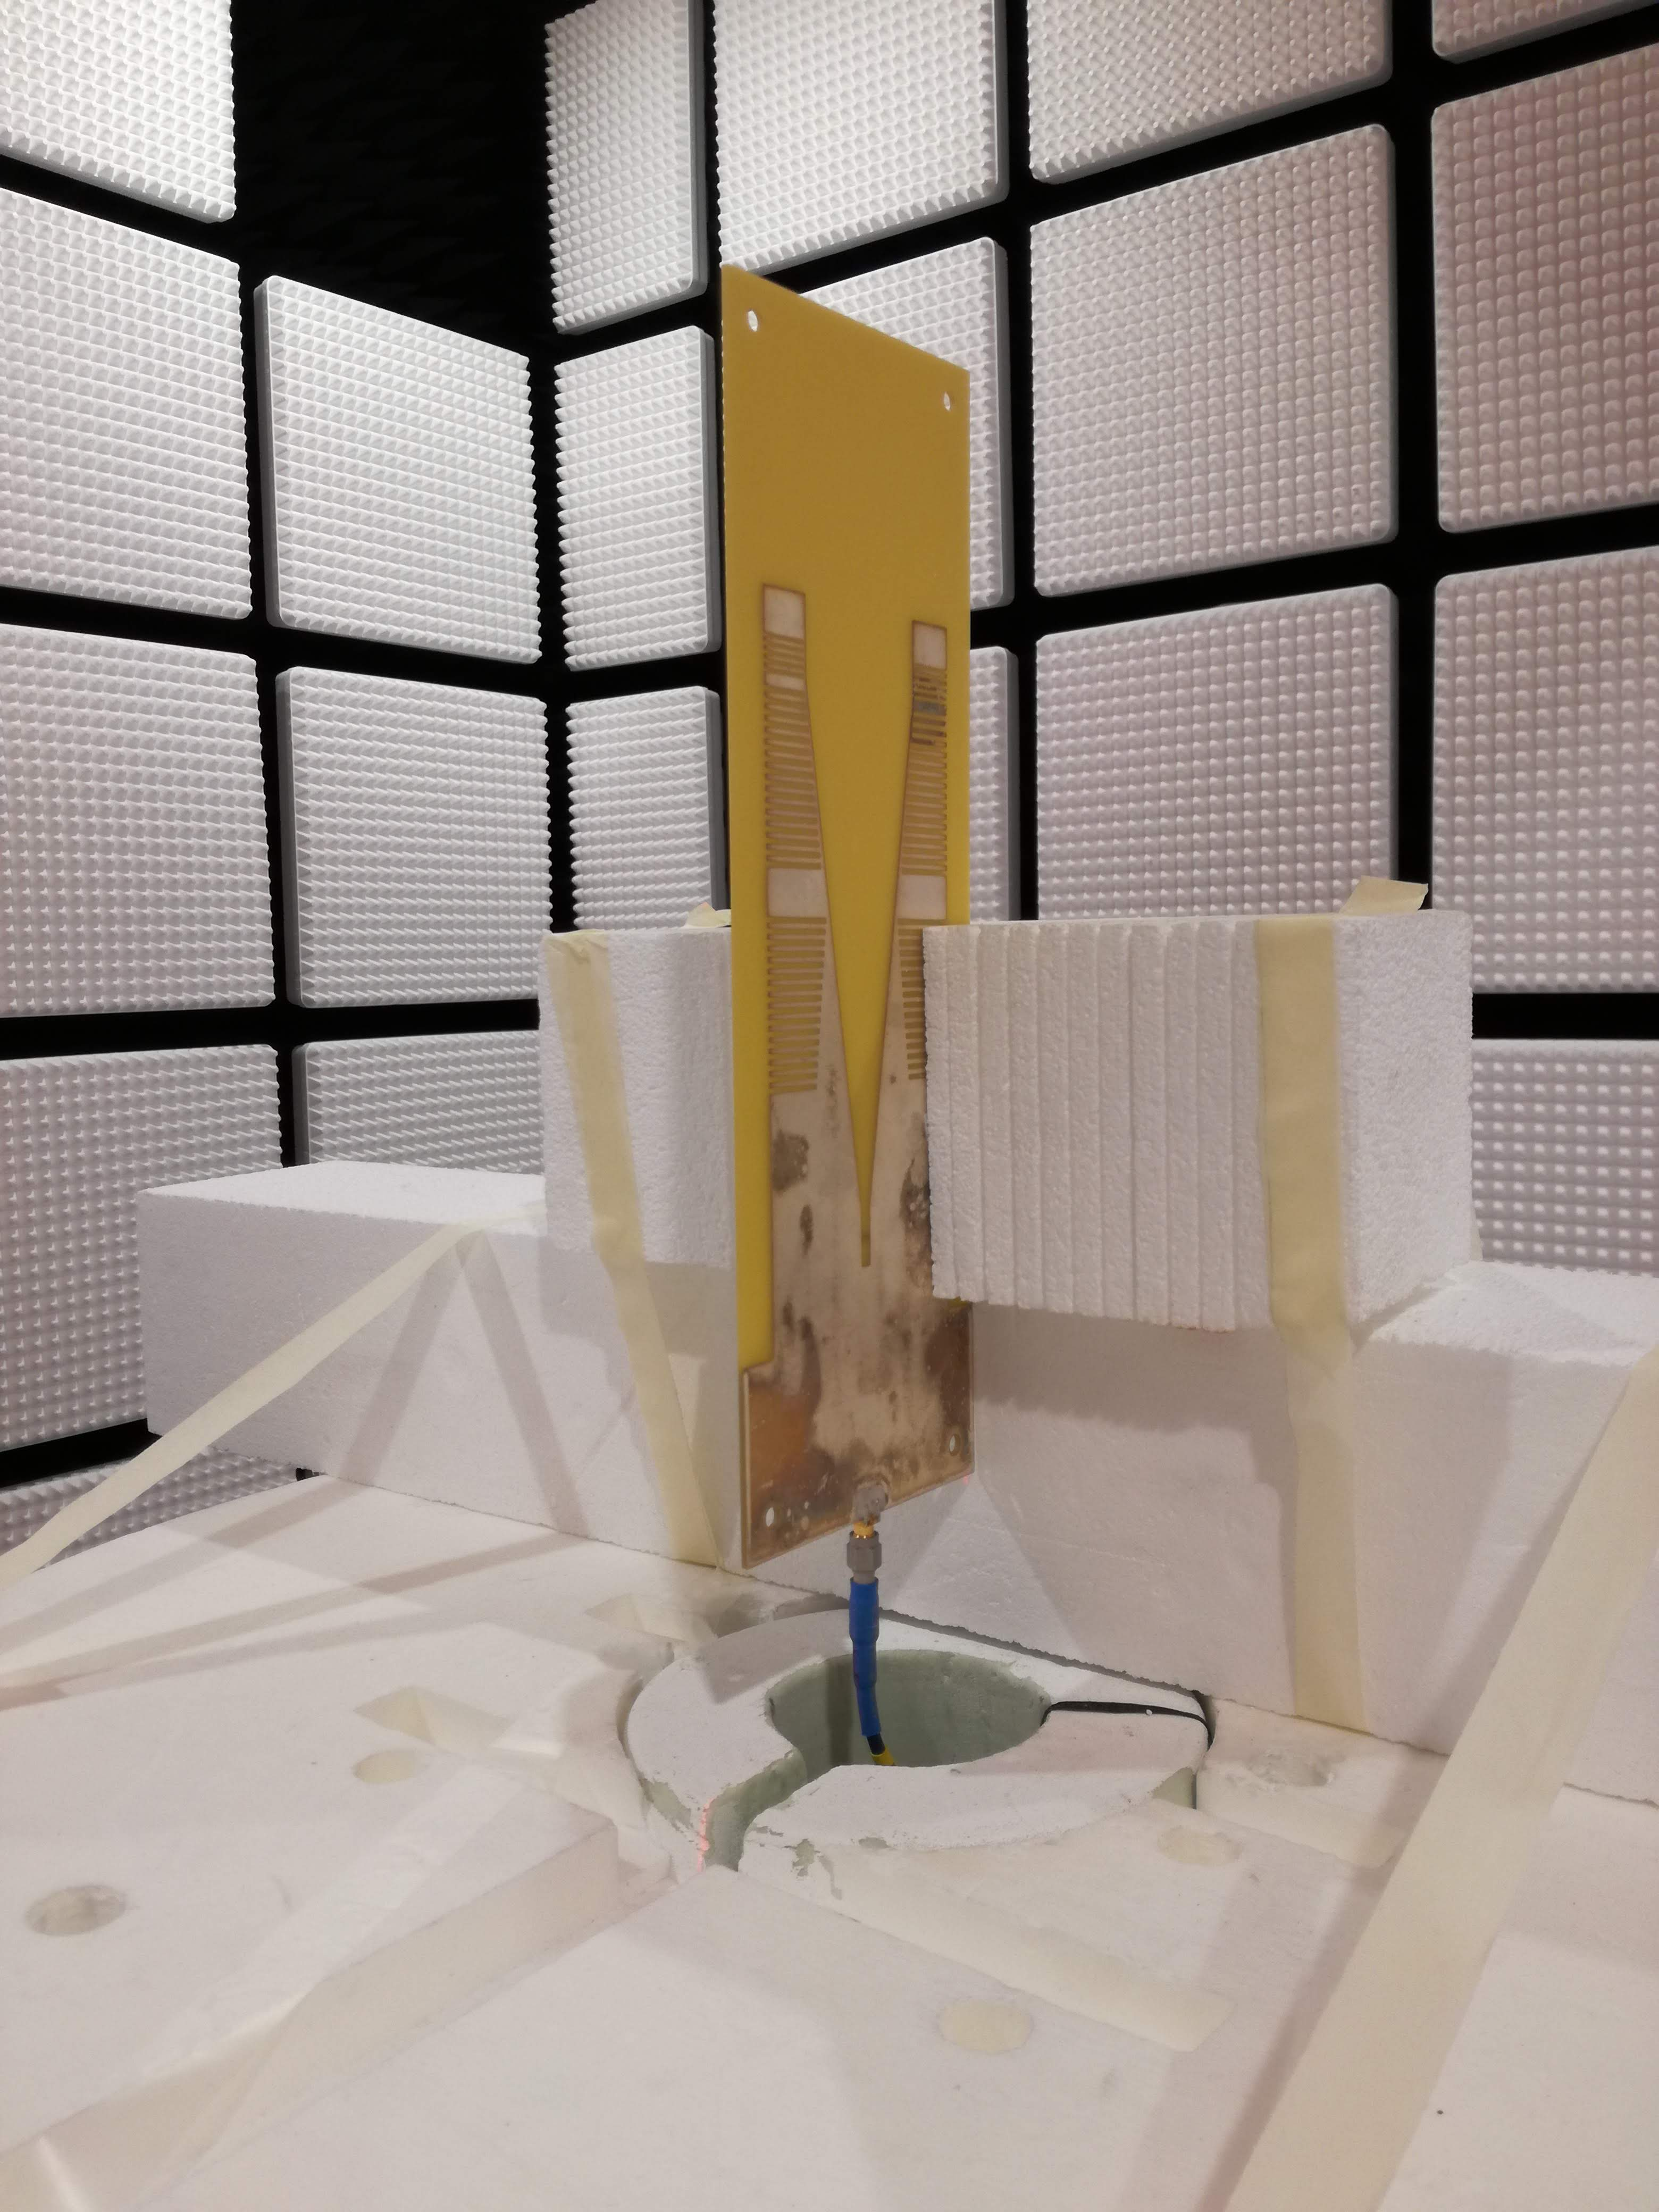
\includegraphics[scale = 0.05]{figures/measurement/antennas/one_ant.jpg}
\caption{Measurement of a single antenna in an anechoic chamber}
\label{fig:chamber_one_ant}
\end{figure} 

\begin{figure}[H]
\centering 
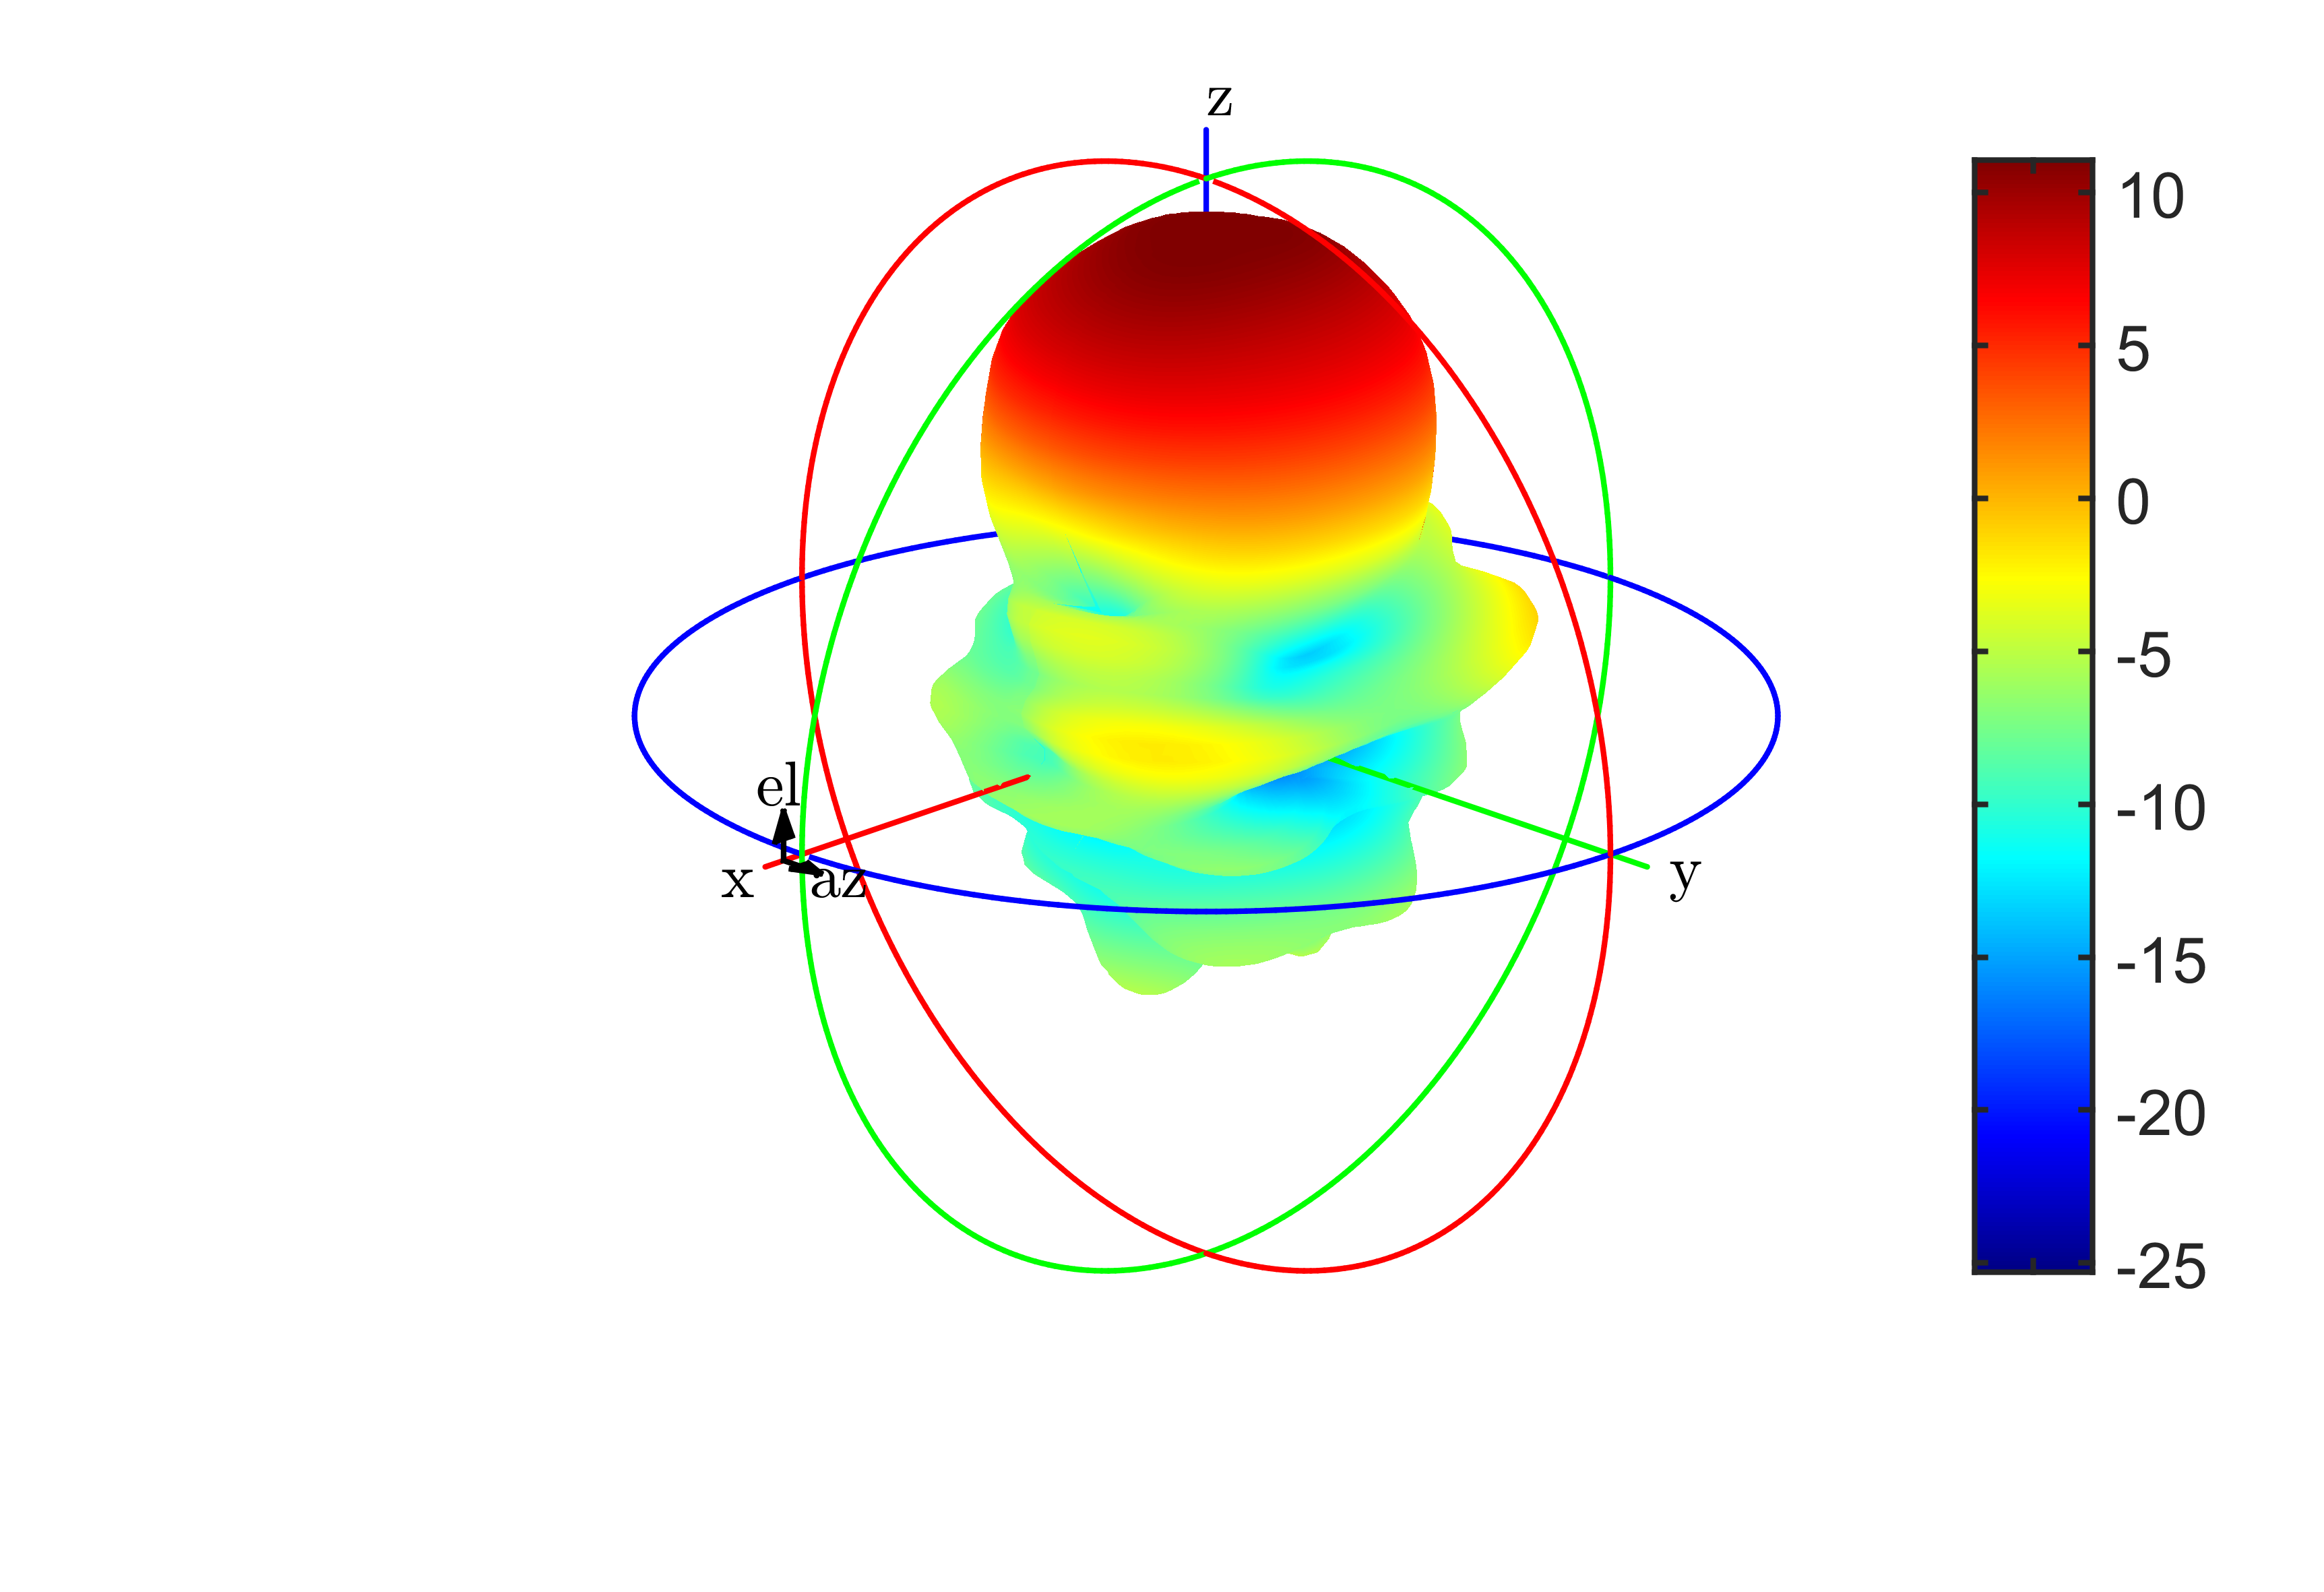
\includegraphics[scale = 0.8]{figures/measurement/antennas/one_ant.png}
\caption{Measured farfield in dB. Maximum gain is 11.1dB}
\label{fig:chamber_one_ant_ff}
\end{figure} 



\begin{figure}[H]
\centering 
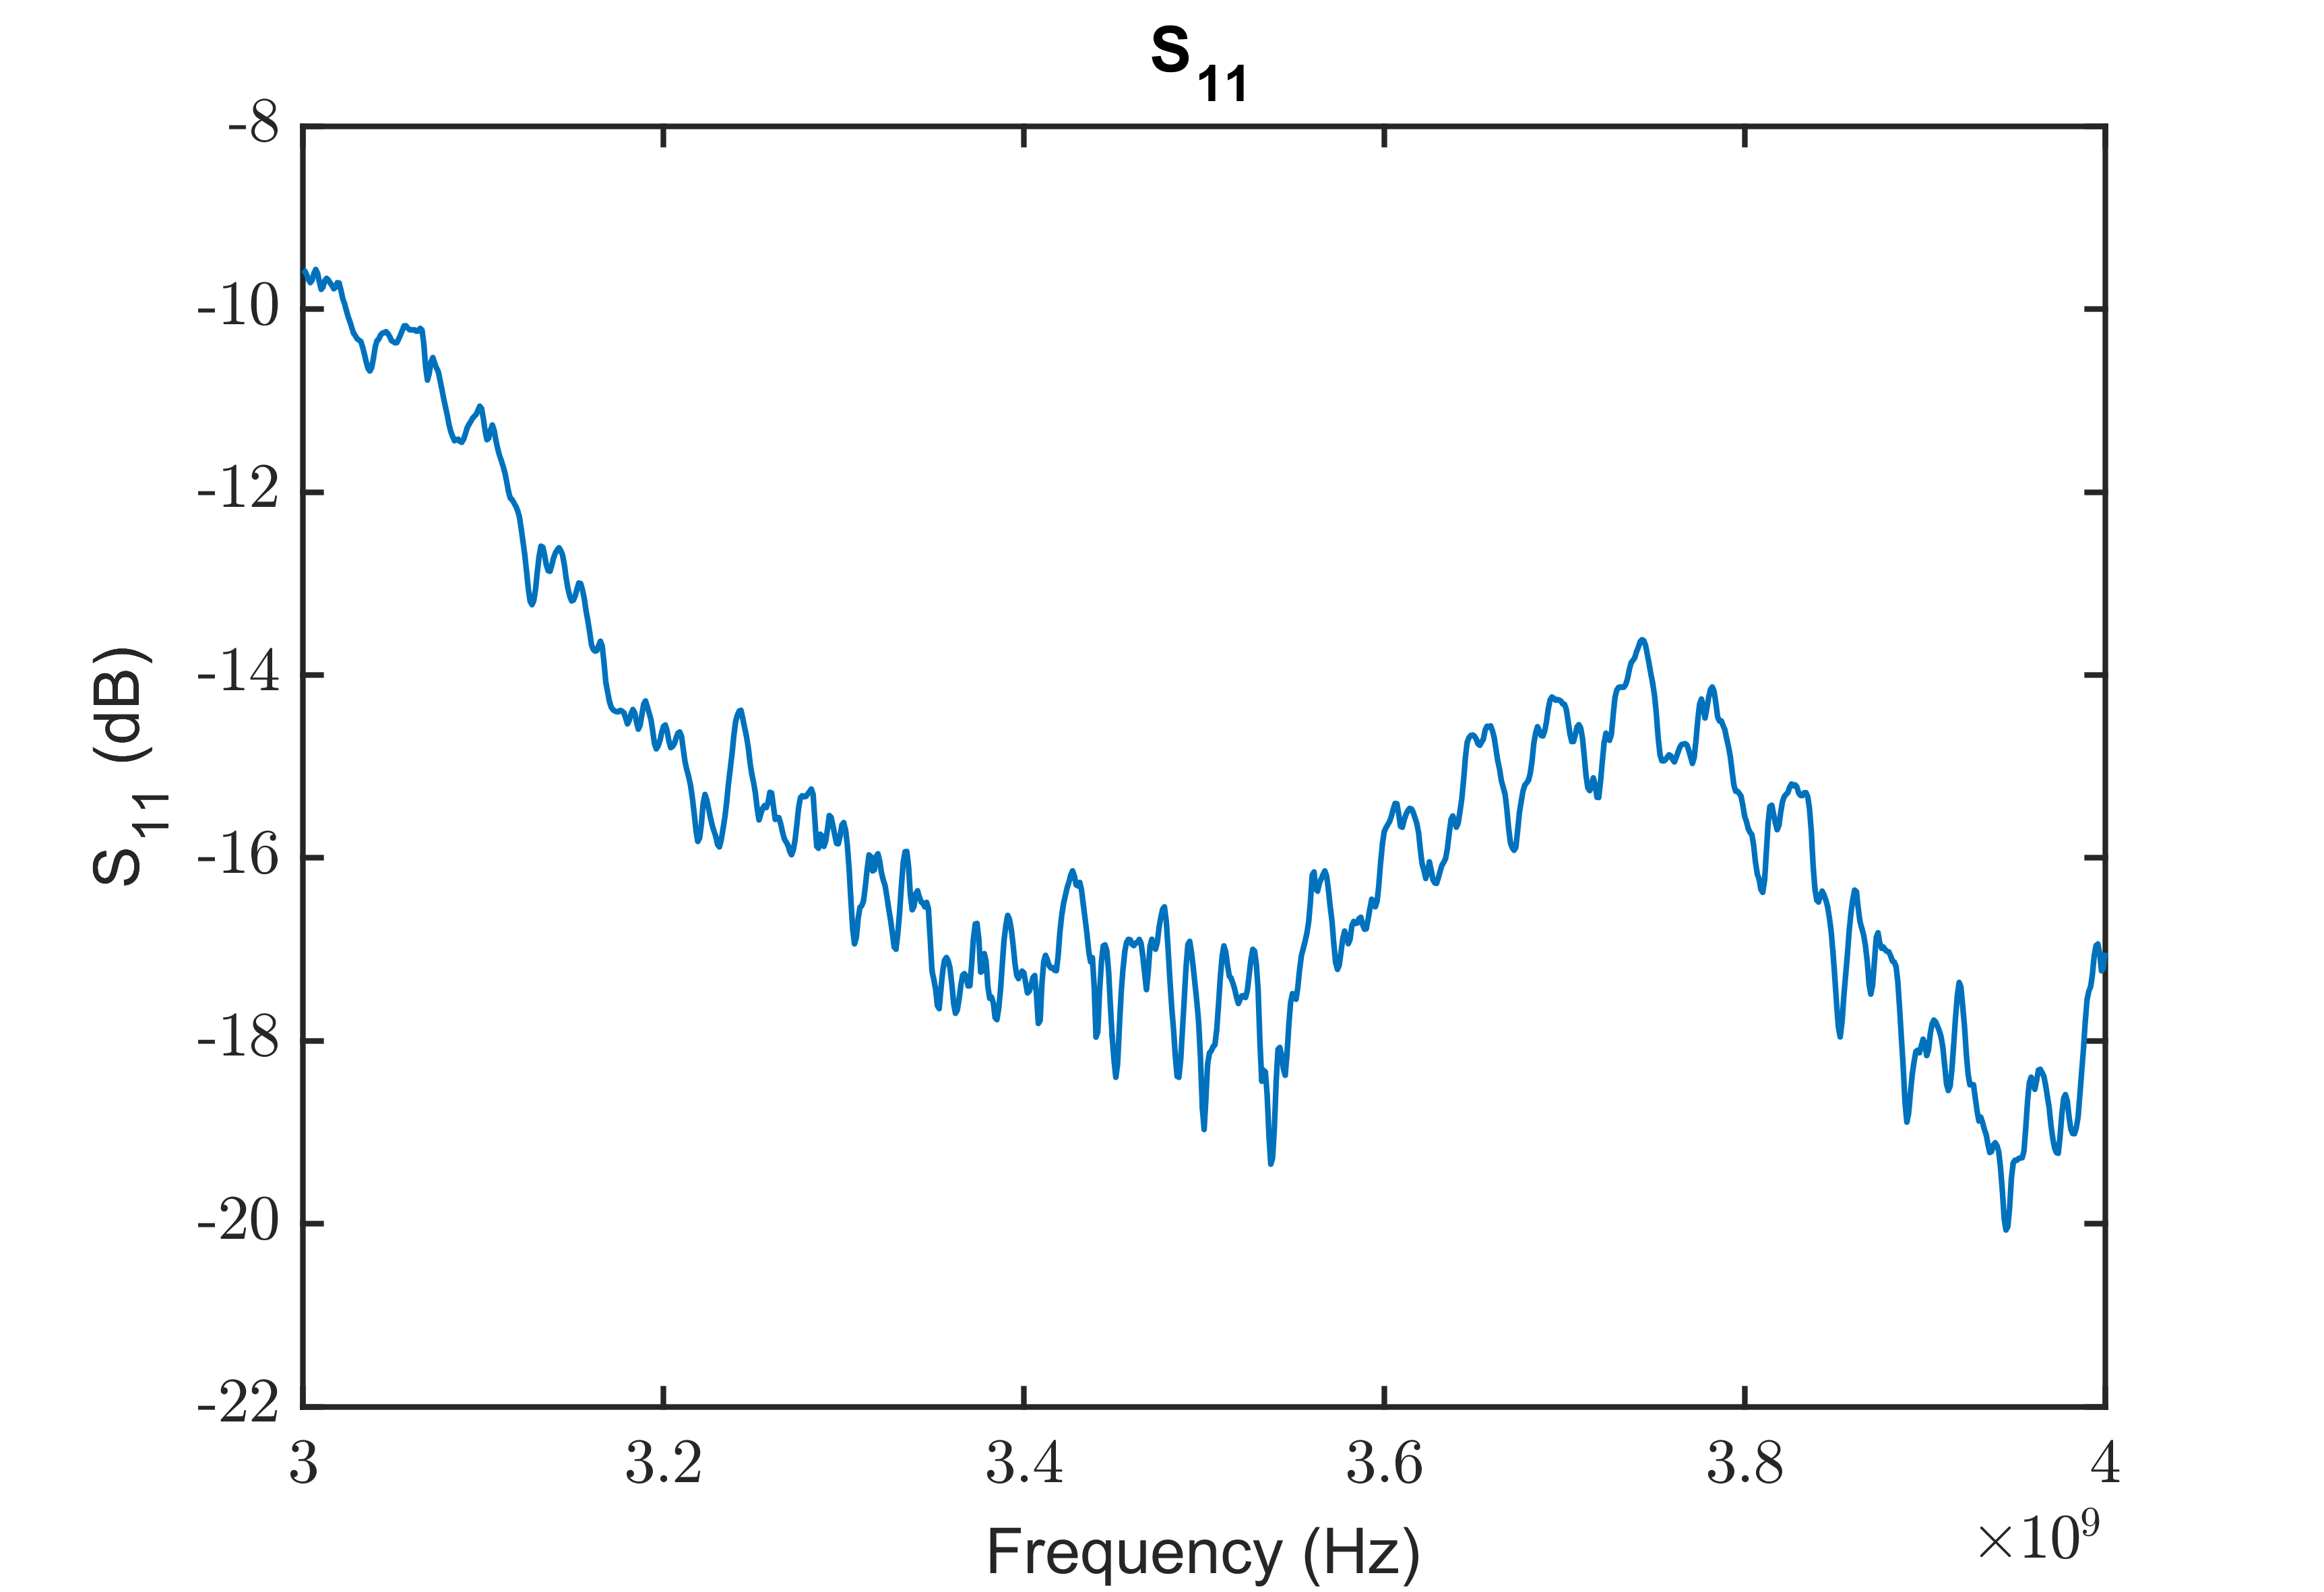
\includegraphics[scale = 0.8]{figures/measurement/antennas/spar_single_ant_s11.png}
\caption{Measured S11 parameter of a single antenna}
\label{fig:chamber_s11}
\end{figure} 

%%%%%%%%%%%%%%%%%%%%%%%%%%%%%%%%%%%%%%%%%%%%%%%%%%%%%%%%%%%%%%%%%%%%%%%%%%%%%%%%%%%%%%%%%%%%%%%%%%%%%%%%%%%%%%%
\section{Two antennas}
In this section measurement is done at two antennas that are spaced at different distances. This is to see how the farfield will change due to coupling of the array. In the theory the gain should become 3dB greater using two antennas than using one antenna, but for this measurement a power divider is used, which is a a 4-port divider that introduces a loss at 6dB to every port. Therefore a decrease of 3dB is expected. The unused ports of the power divider is terminated to a $50\Omega$ load. It is seen from figure \ref{fig:chamber_two_ant_ff_01} to \ref{fig:chamber_two_ant_ff:06} that the farfield flattens in the y direction and that the gain varies with the distances between the elements. The loss seems to be lower than expected since a loss at only 2.2dB is obtained at $d=0.5\lambda$. The S-parameters is presented in figure \ref{fig:chamber_two_ant_s11} to \ref{fig:chamber_two_ant_s21}. It is seen that as expected $S_{11}$ and $S_{22}$ are similar and that $S_{12}$ and $S_{21}$ also are similar. It is seen that the return-loss $S_{11}$ and $S_{22}$ changes a lot with the spacing of the antennas. The largest difference is seen from 0.1 to 0.3 wavelengths. This is also seen from the coupling $S_{12}$ and $S_{21}$ that at 0.1 and 0.2 wavelengths ther is a large amount of coupling. 

\begin{figure}[H]
\centering 
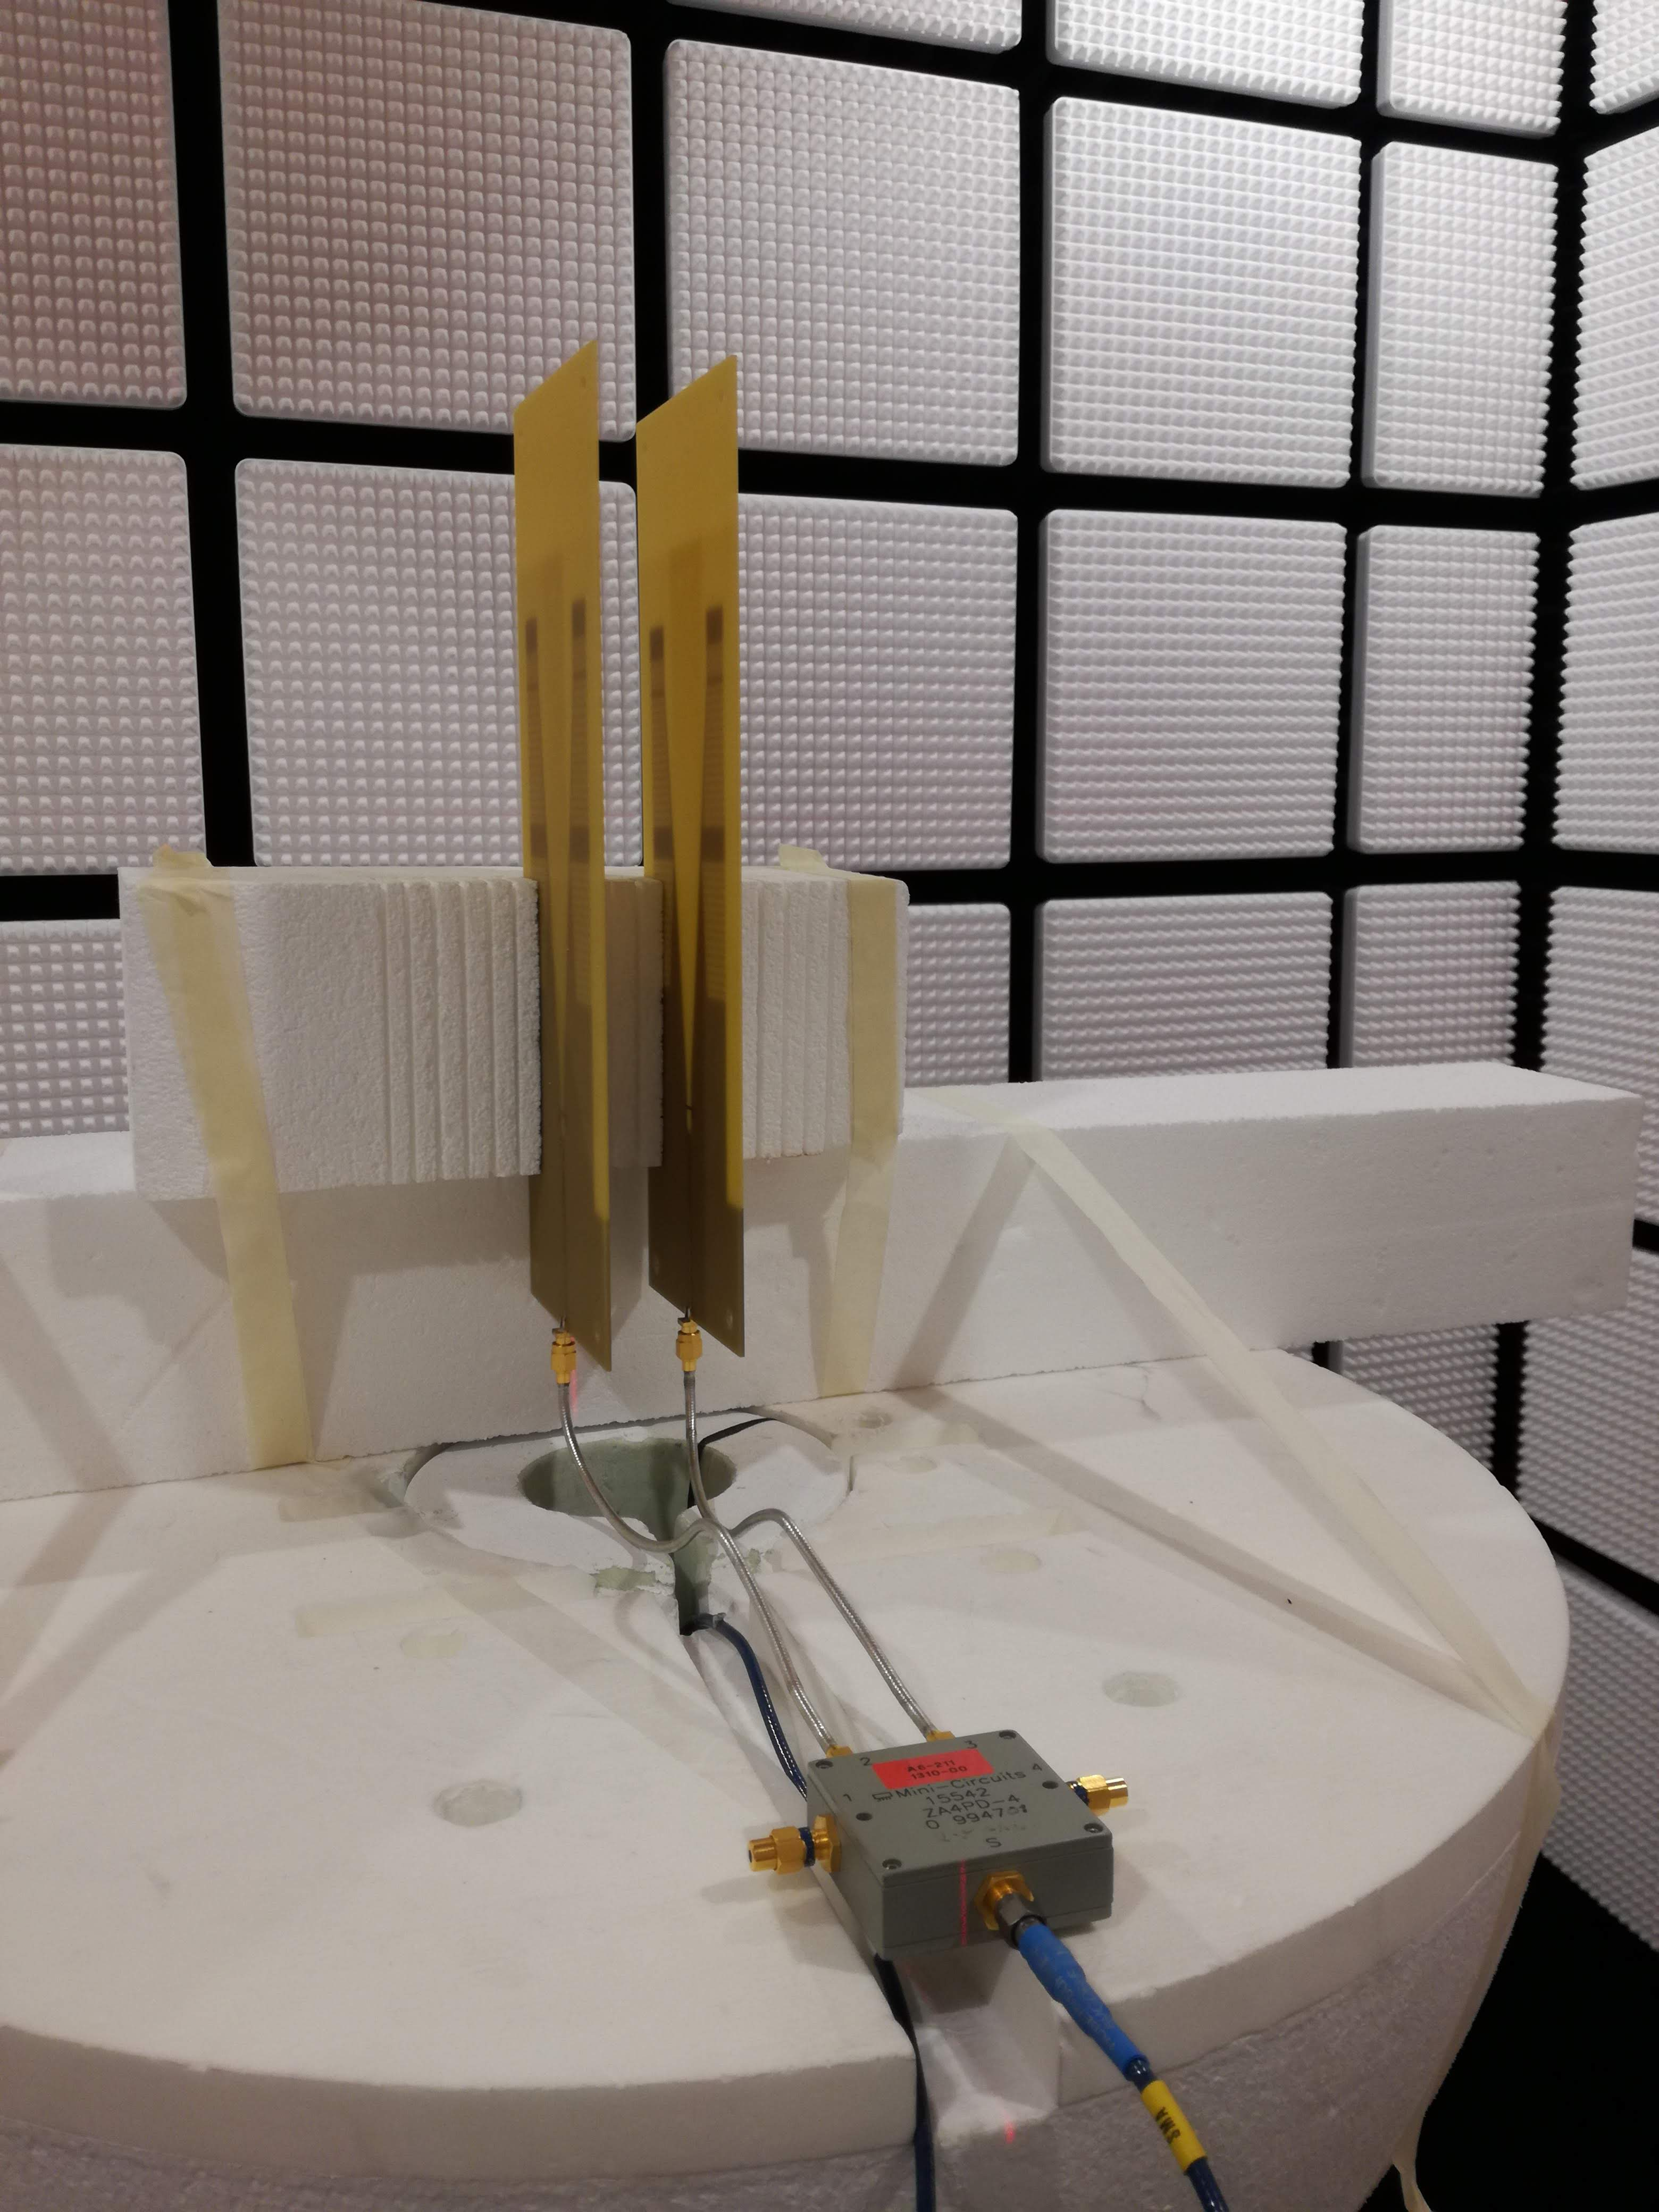
\includegraphics[scale = 0.05]{figures/measurement/antennas/two_ant.jpg}
\caption{Measurement of two antennas with a powerdivider in an anechoic chamber. The distances between the antennas are varied for every measurement. The distance is $0.5\lambda$ on the picture}
\label{fig:chamber_two_ant}
\end{figure} 


\begin{figure}[H]
  \centering
  \begin{minipage}[b]{0.5\textwidth}
	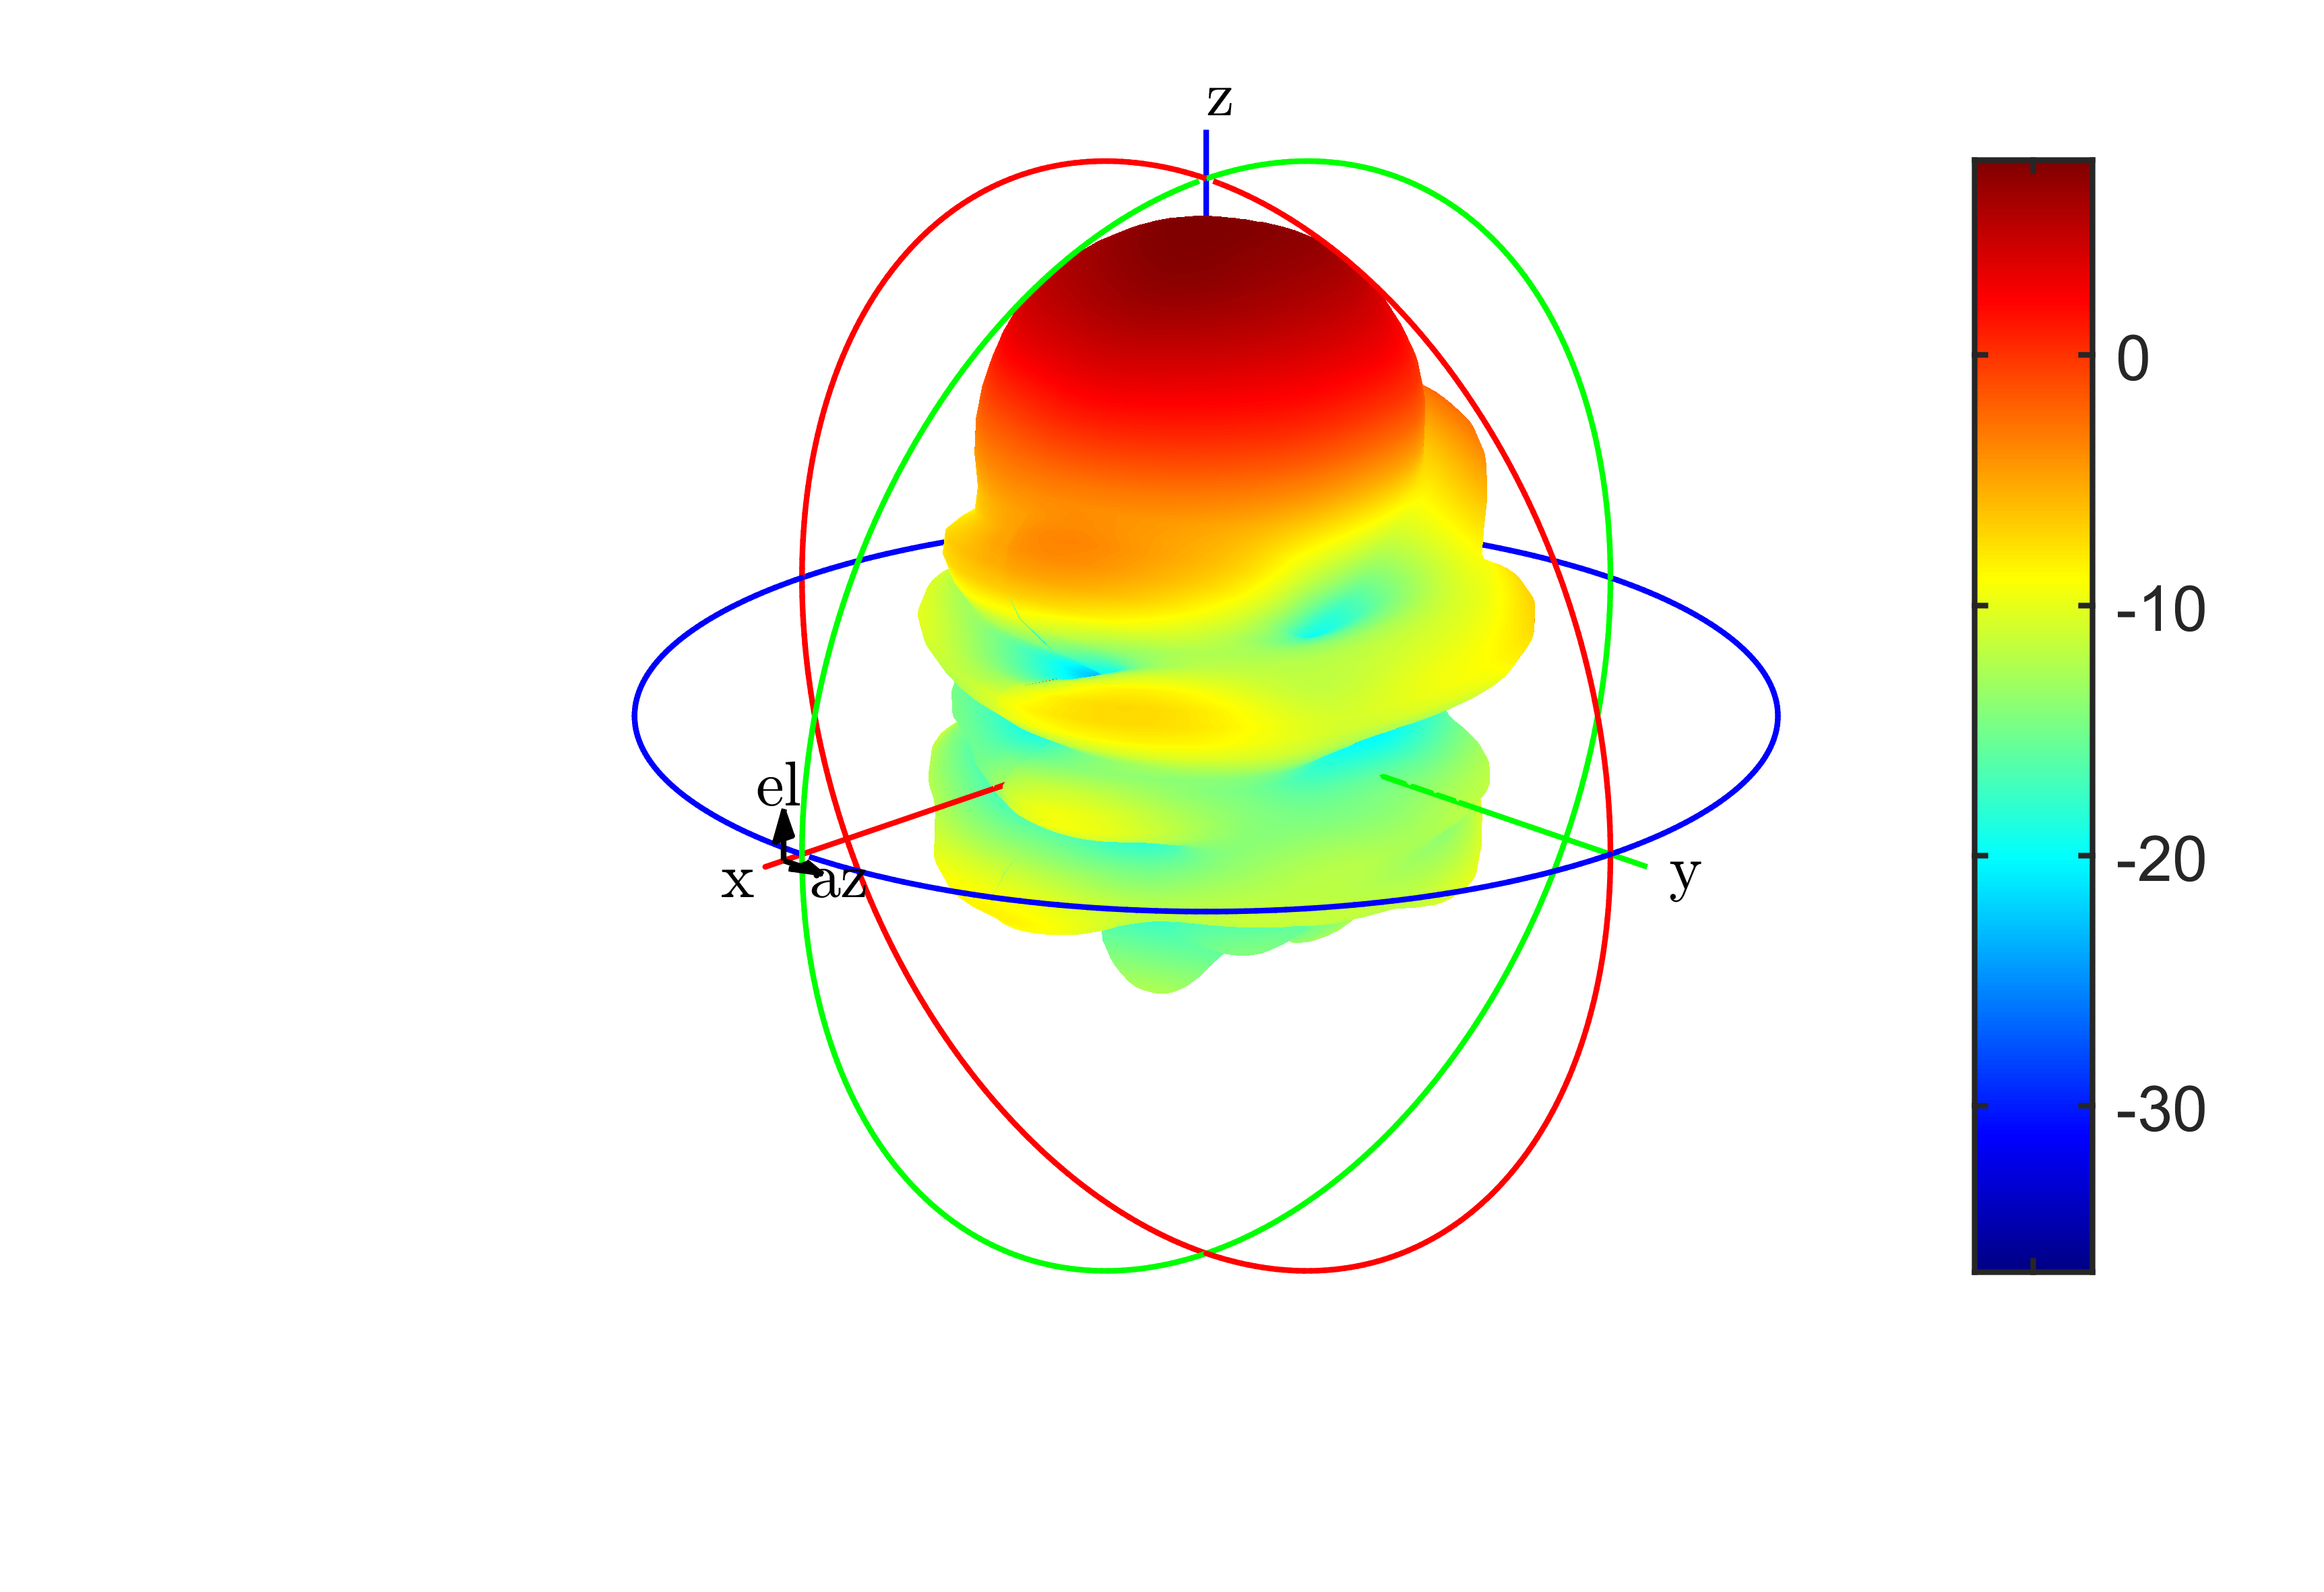
\includegraphics[scale = 0.5]{figures/measurement/antennas/array_2_0p1.png}
	\caption{Farfield for $d = 0.1\lambda$. Maximum gain is 7.8dB}
    \label{fig:chamber_two_ant_ff_01}
  \end{minipage}
  \hfill
  \begin{minipage}[b]{0.4\textwidth}
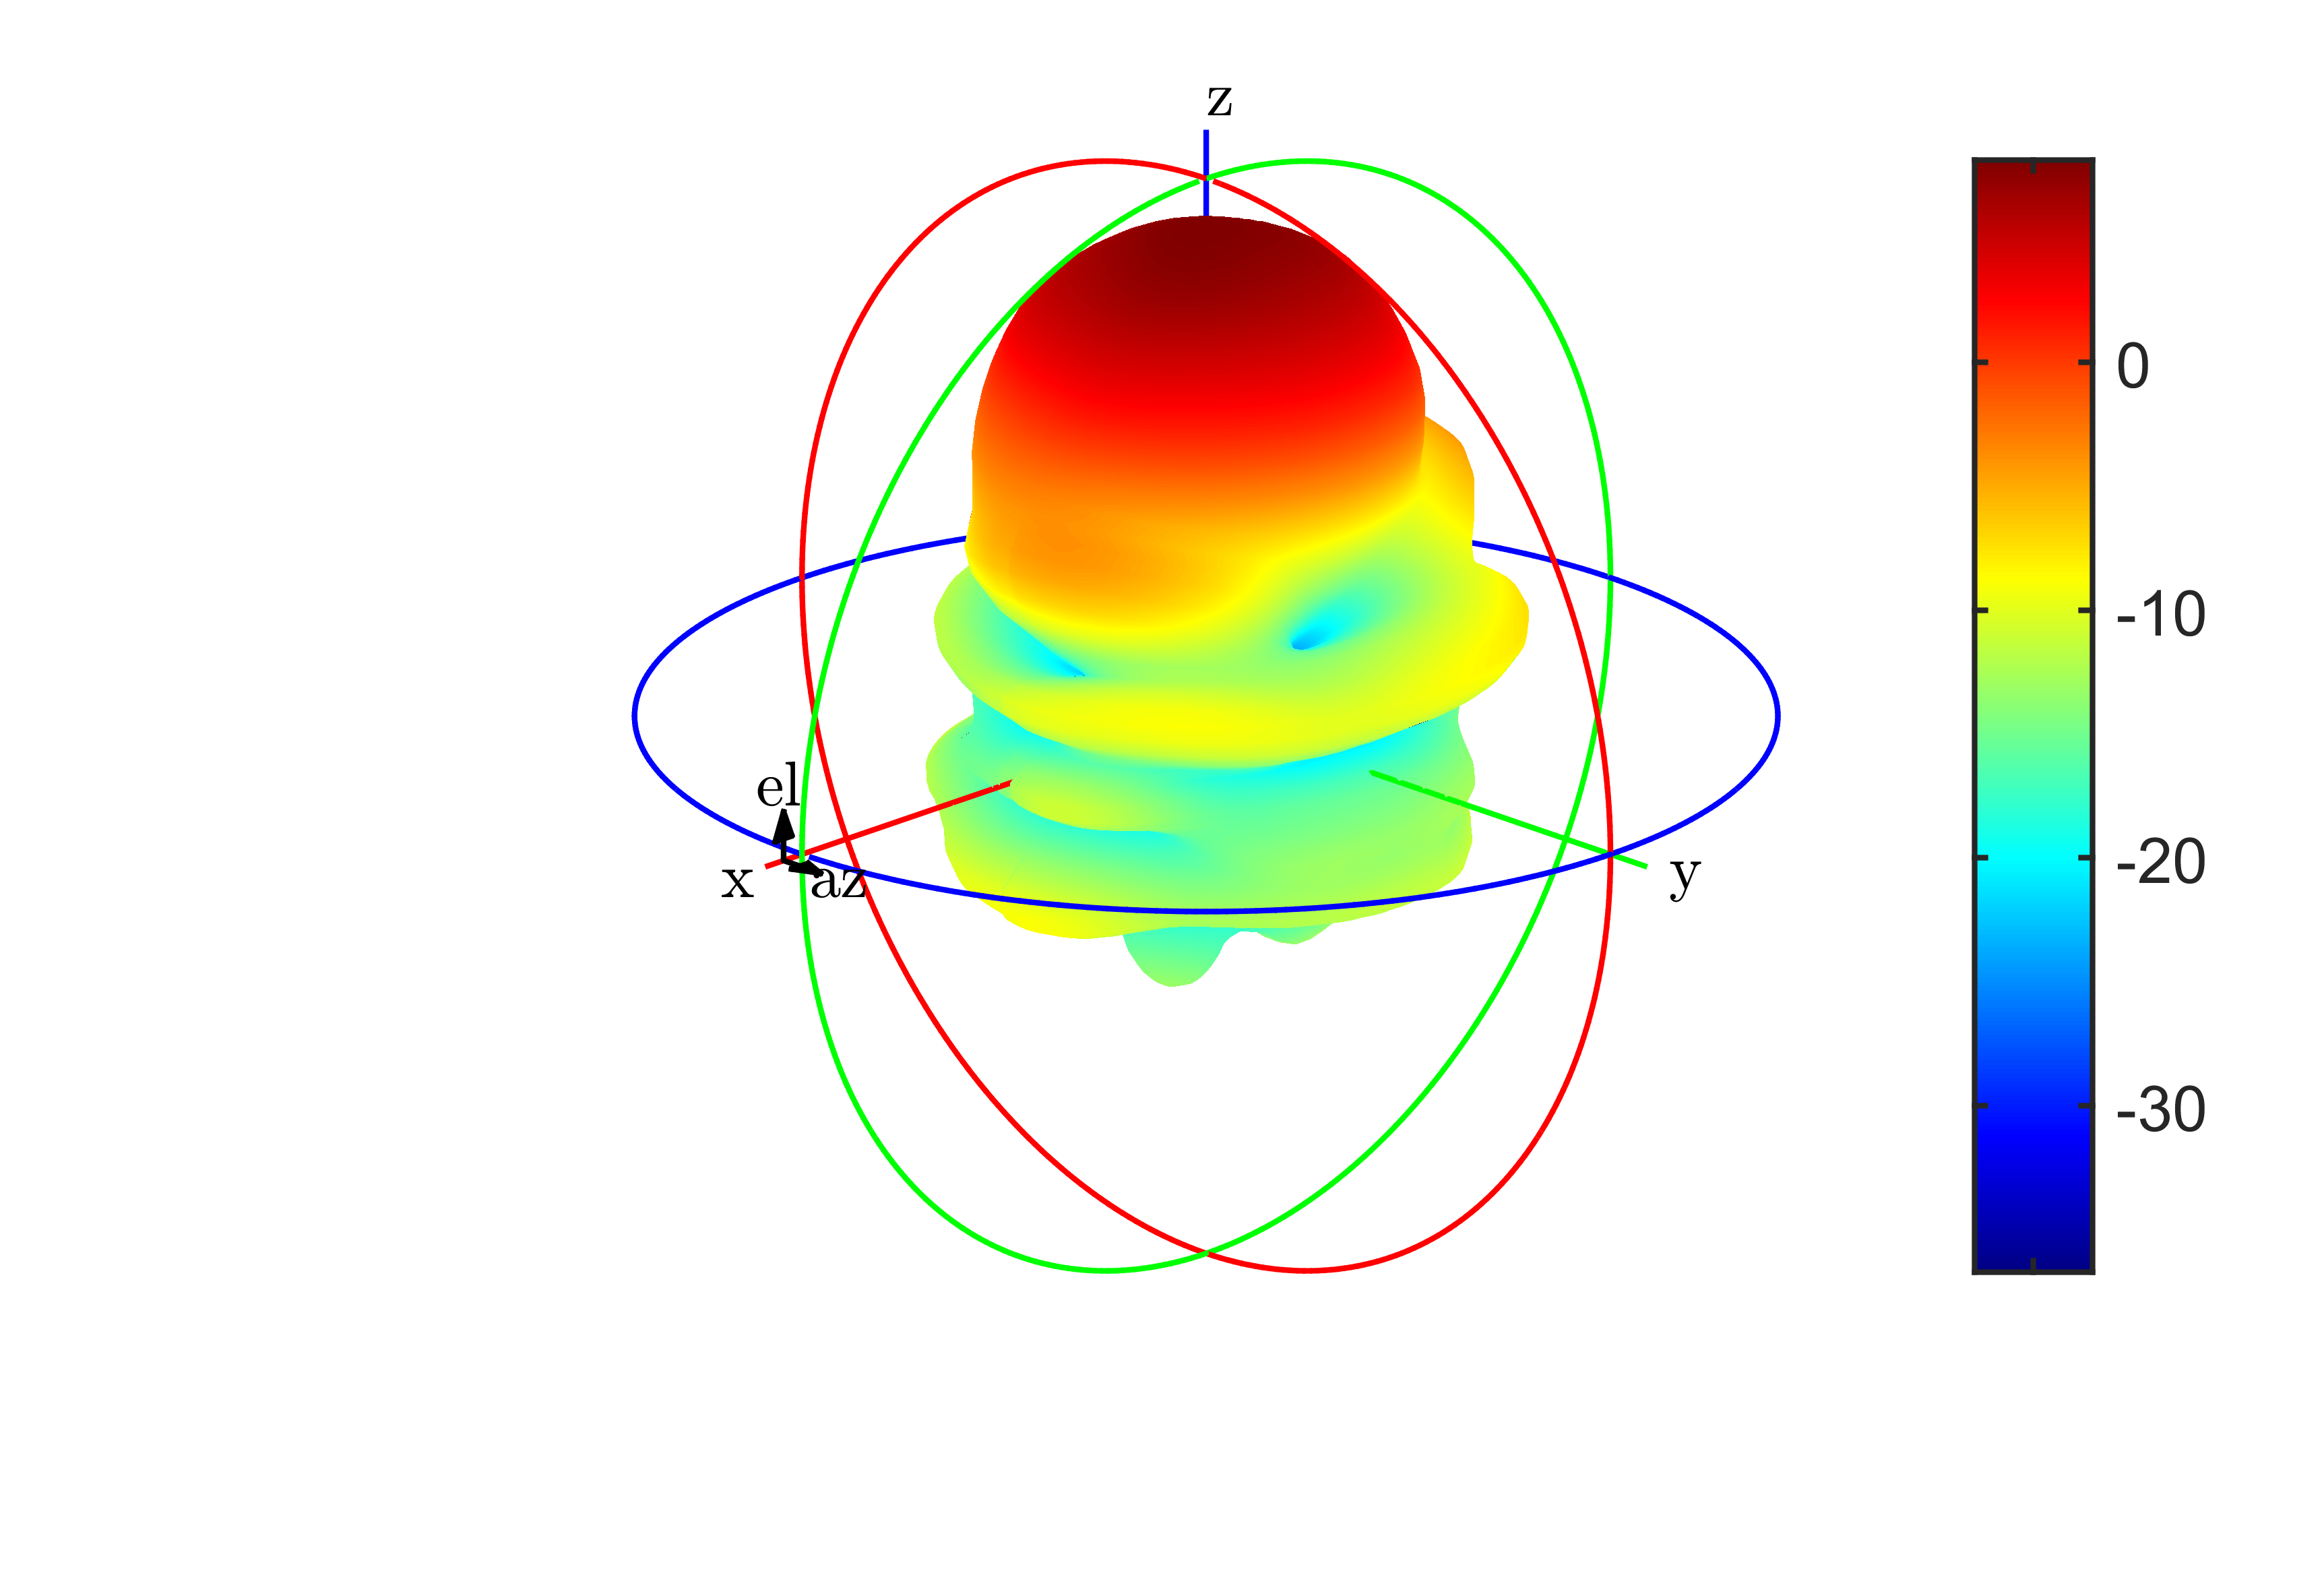
\includegraphics[scale = 0.5]{figures/measurement/antennas/array_2_0p2.png}
\caption{Farfield for $d = 0.2\lambda$. Maximum gain is 8.2dB}
    \label{fig:chamber_two_ant_ff:02}
  \end{minipage}
\end{figure}

\begin{figure}[H]
  \centering
  \begin{minipage}[b]{0.5\textwidth}
	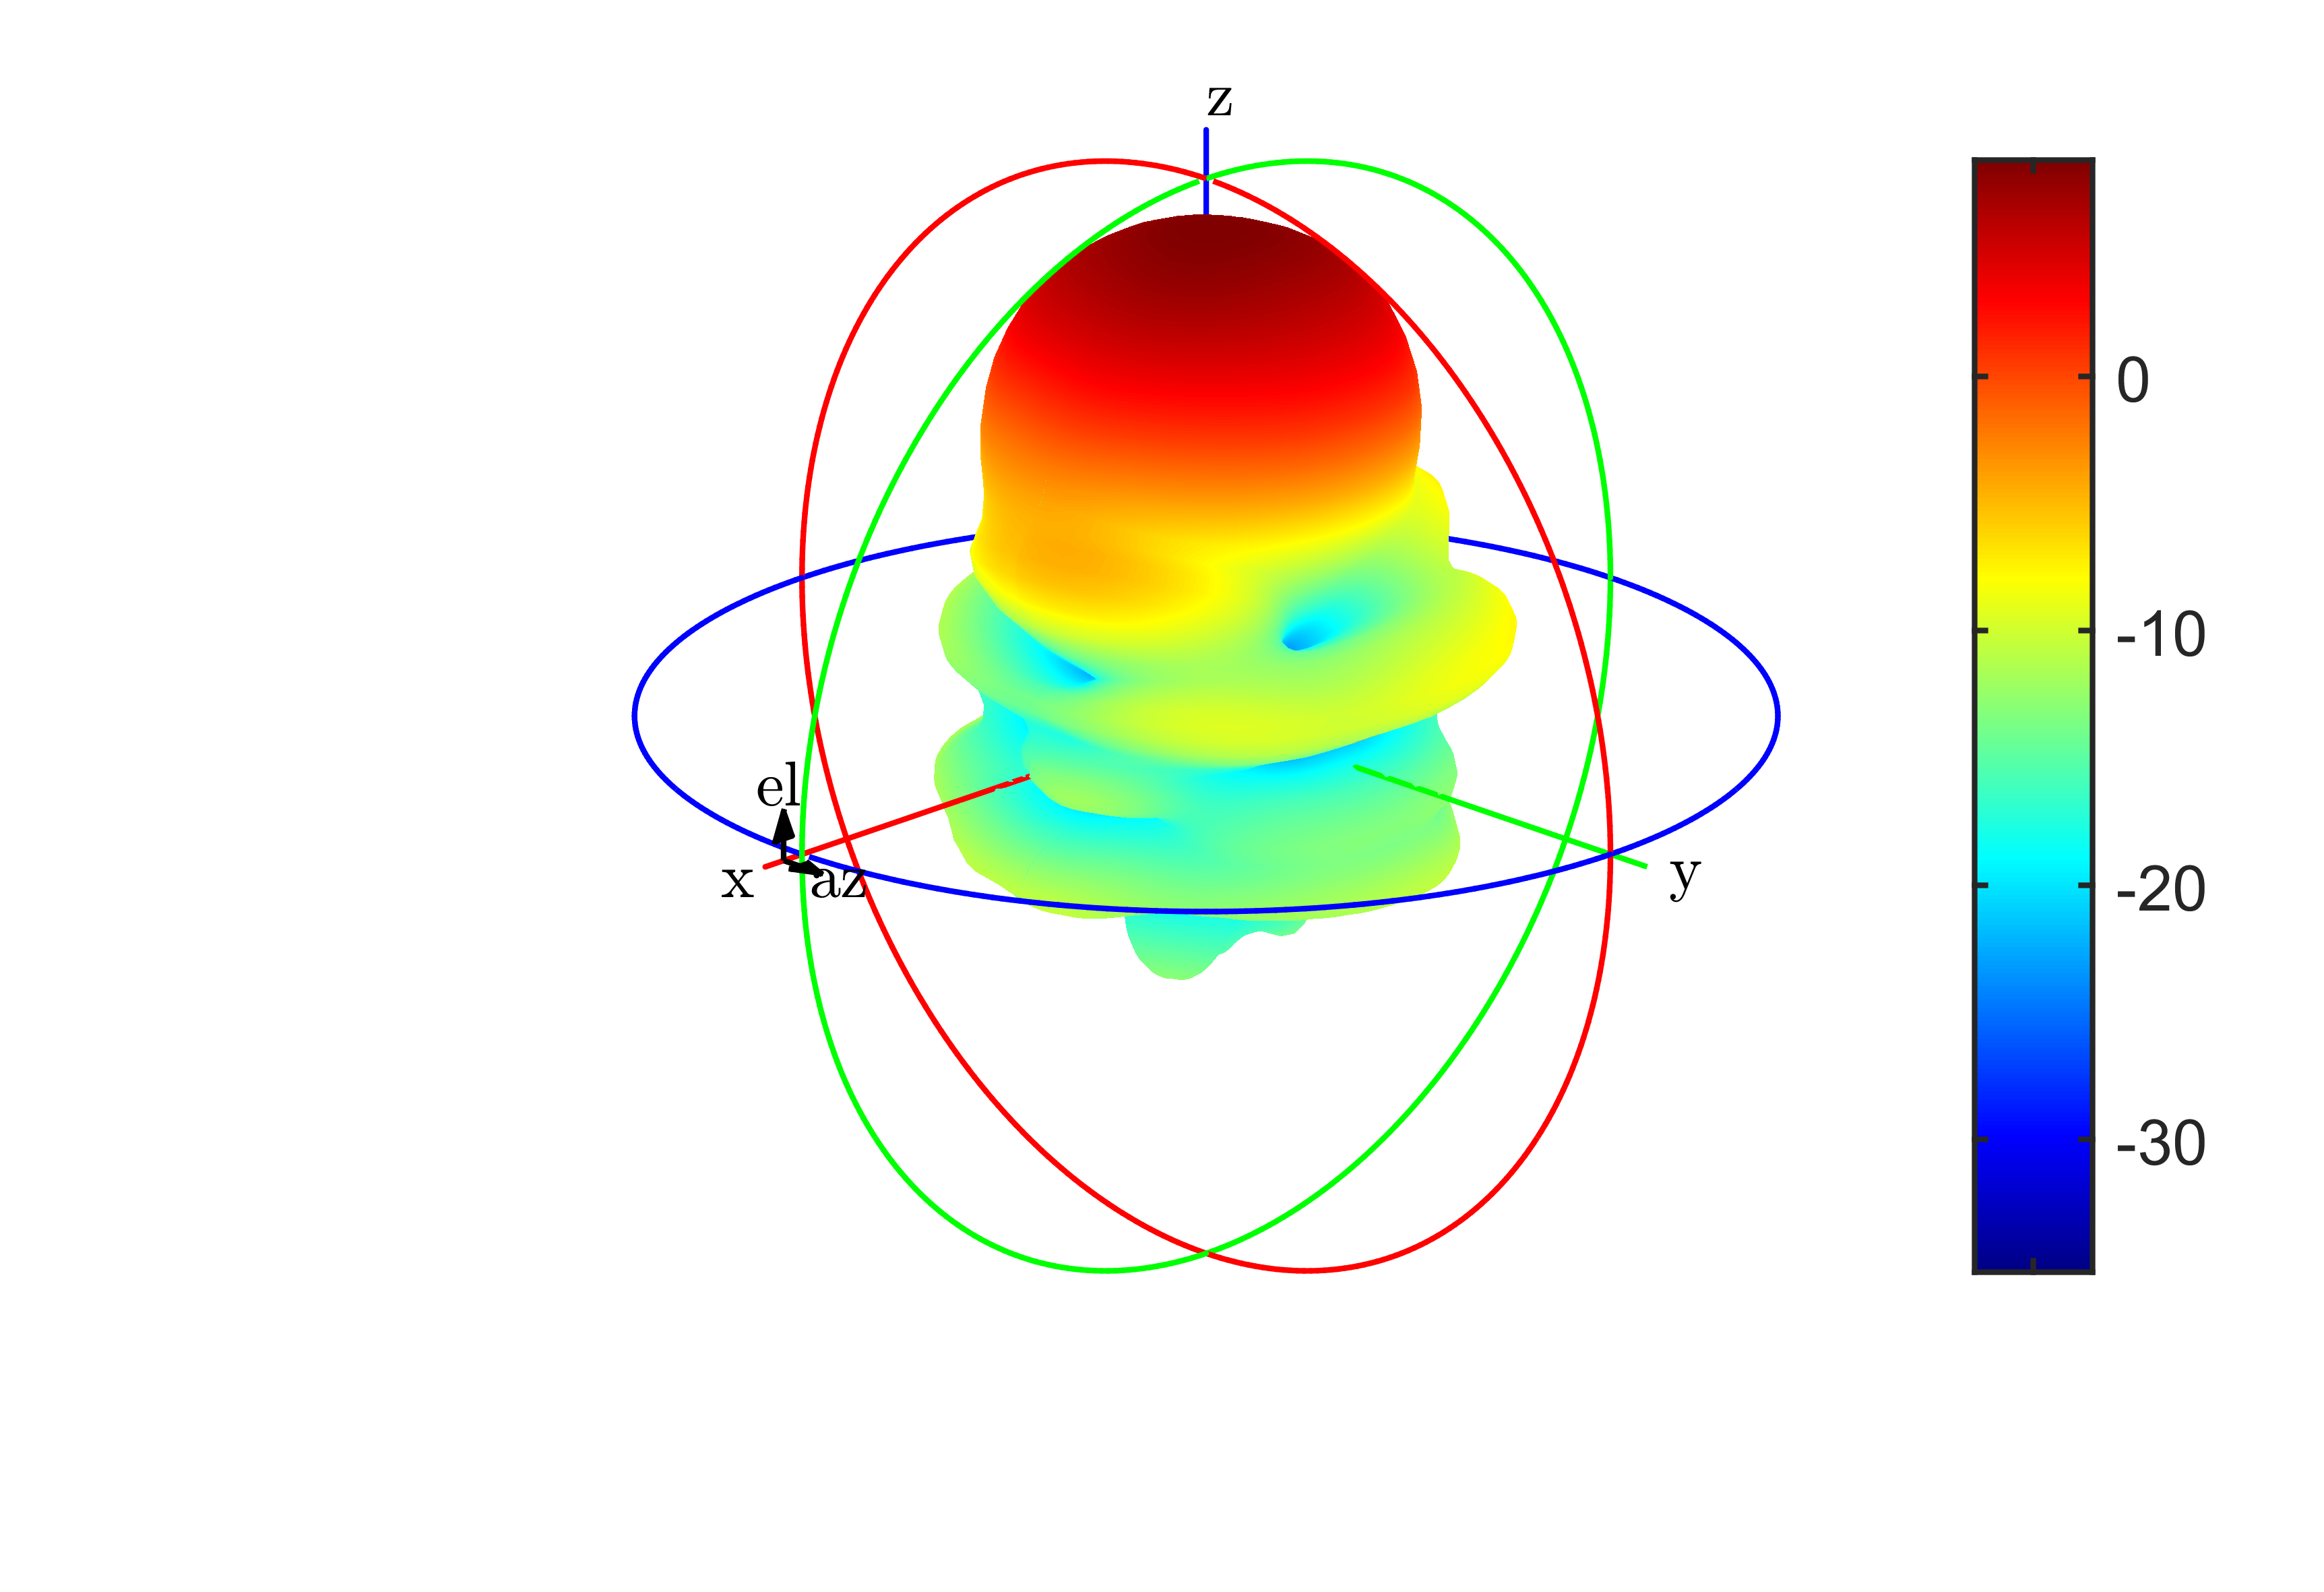
\includegraphics[scale = 0.5]{figures/measurement/antennas/array_2_0p3.png}
	\caption{Farfield for $d = 0.3\lambda$. Maximum gain is 8.5dB}
    \label{fig:chamber_two_ant_ff_03}
  \end{minipage}
  \hfill
  \begin{minipage}[b]{0.4\textwidth}
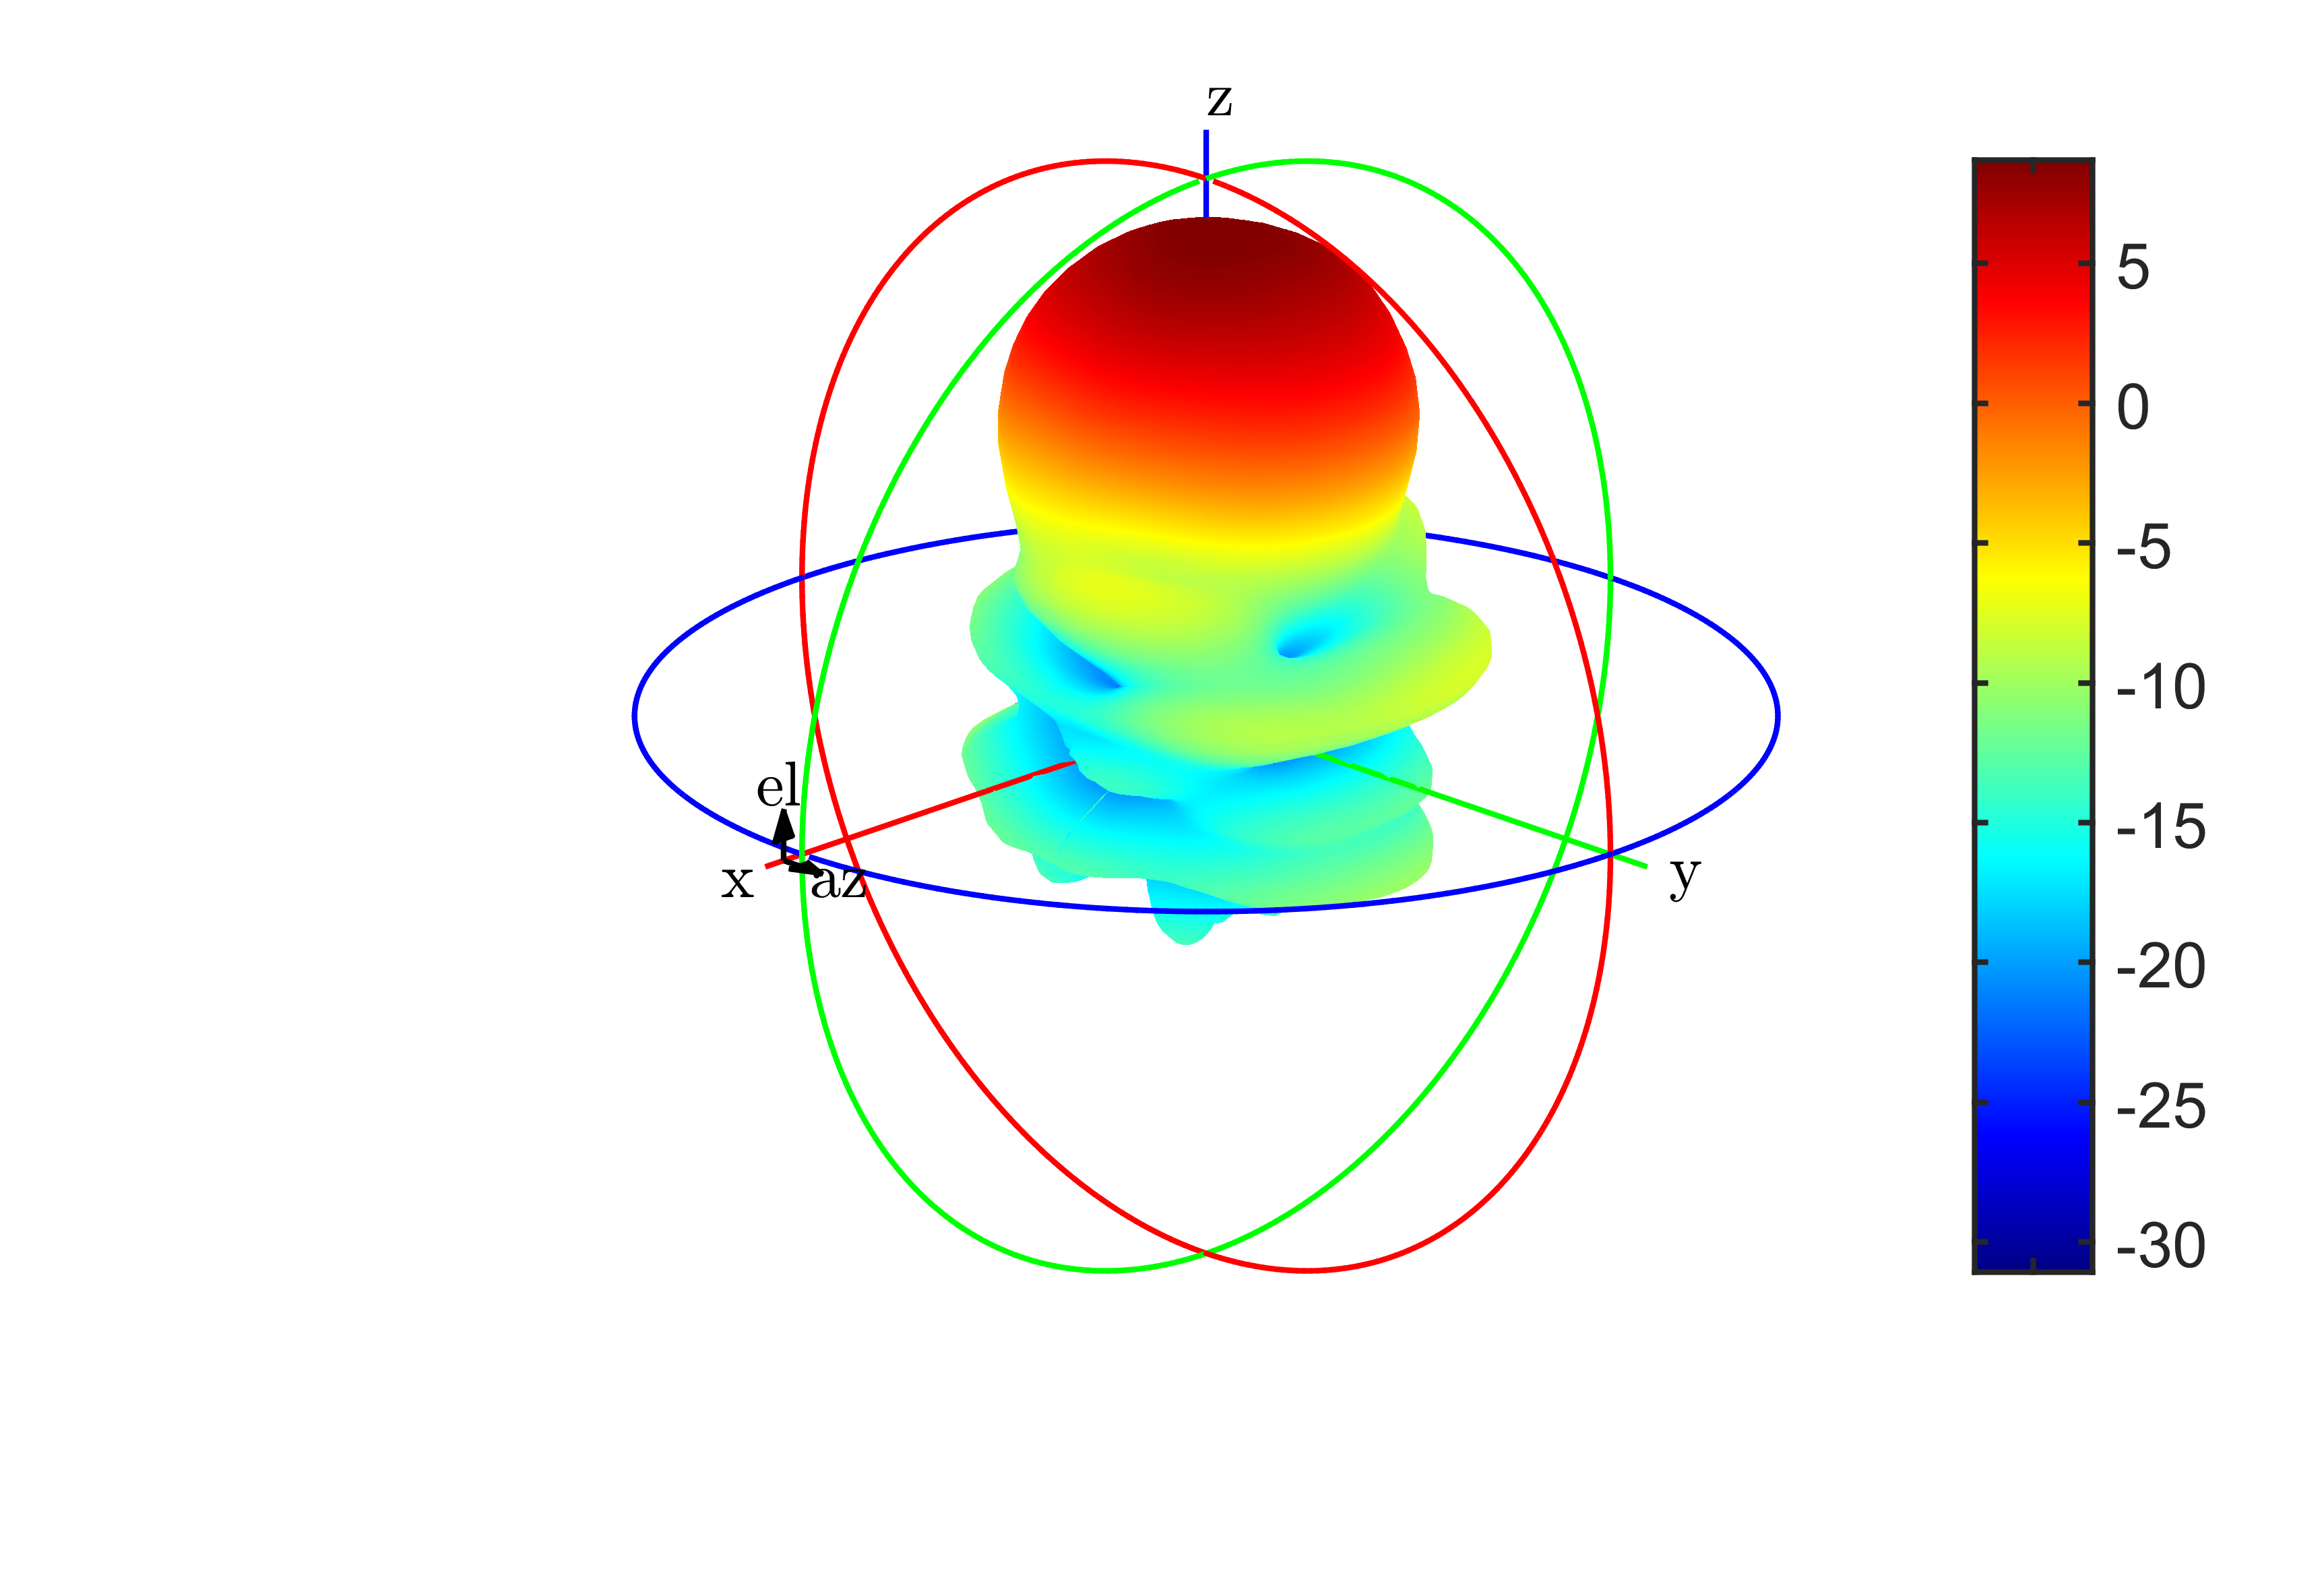
\includegraphics[scale = 0.5]{figures/measurement/antennas/array_2_0p4.png}
\caption{Farfield for $d = 0.4\lambda$. Maximum gain is 8.7dB}
    \label{fig:chamber_two_ant_ff:04}
  \end{minipage}
\end{figure}

\begin{figure}[H]
  \centering
  \begin{minipage}[b]{0.5\textwidth}
	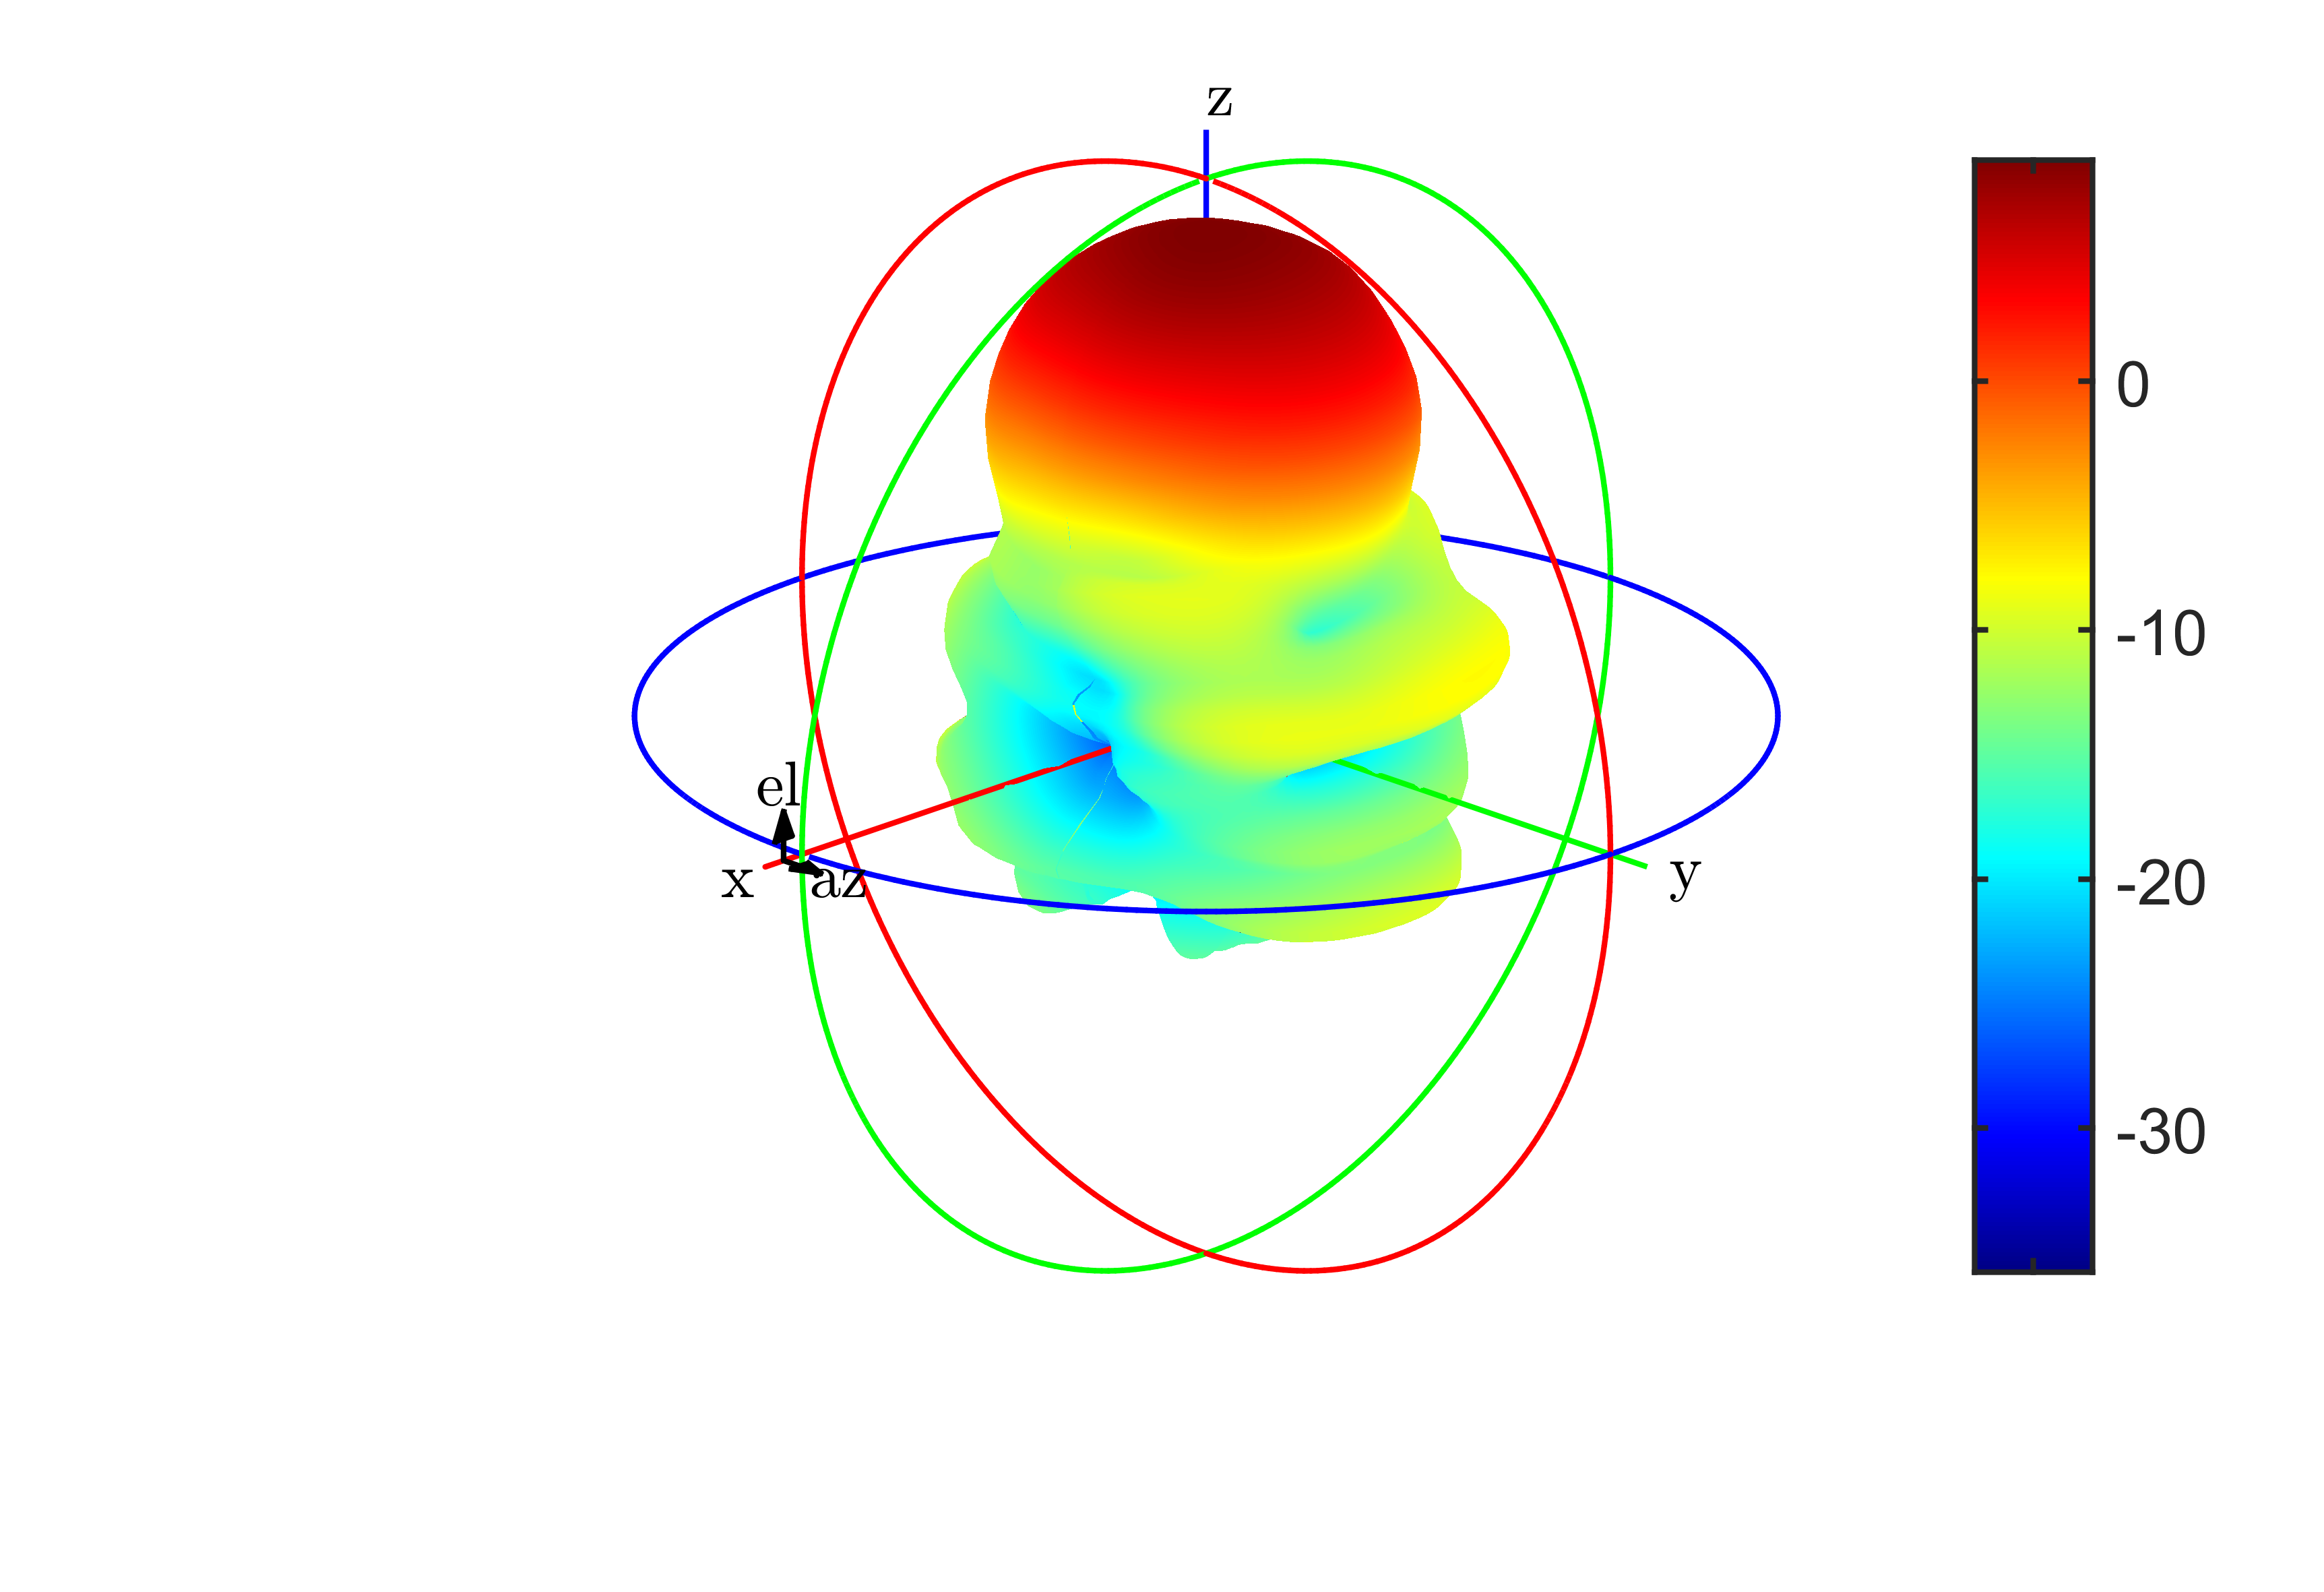
\includegraphics[scale = 0.5]{figures/measurement/antennas/array_2_0p5.png}
	\caption{Farfield for $d = 0.5\lambda$. Maximum gain is 8.9dB}
    \label{fig:chamber_two_ant_ff_05}
  \end{minipage}
  \hfill
  \begin{minipage}[b]{0.4\textwidth}
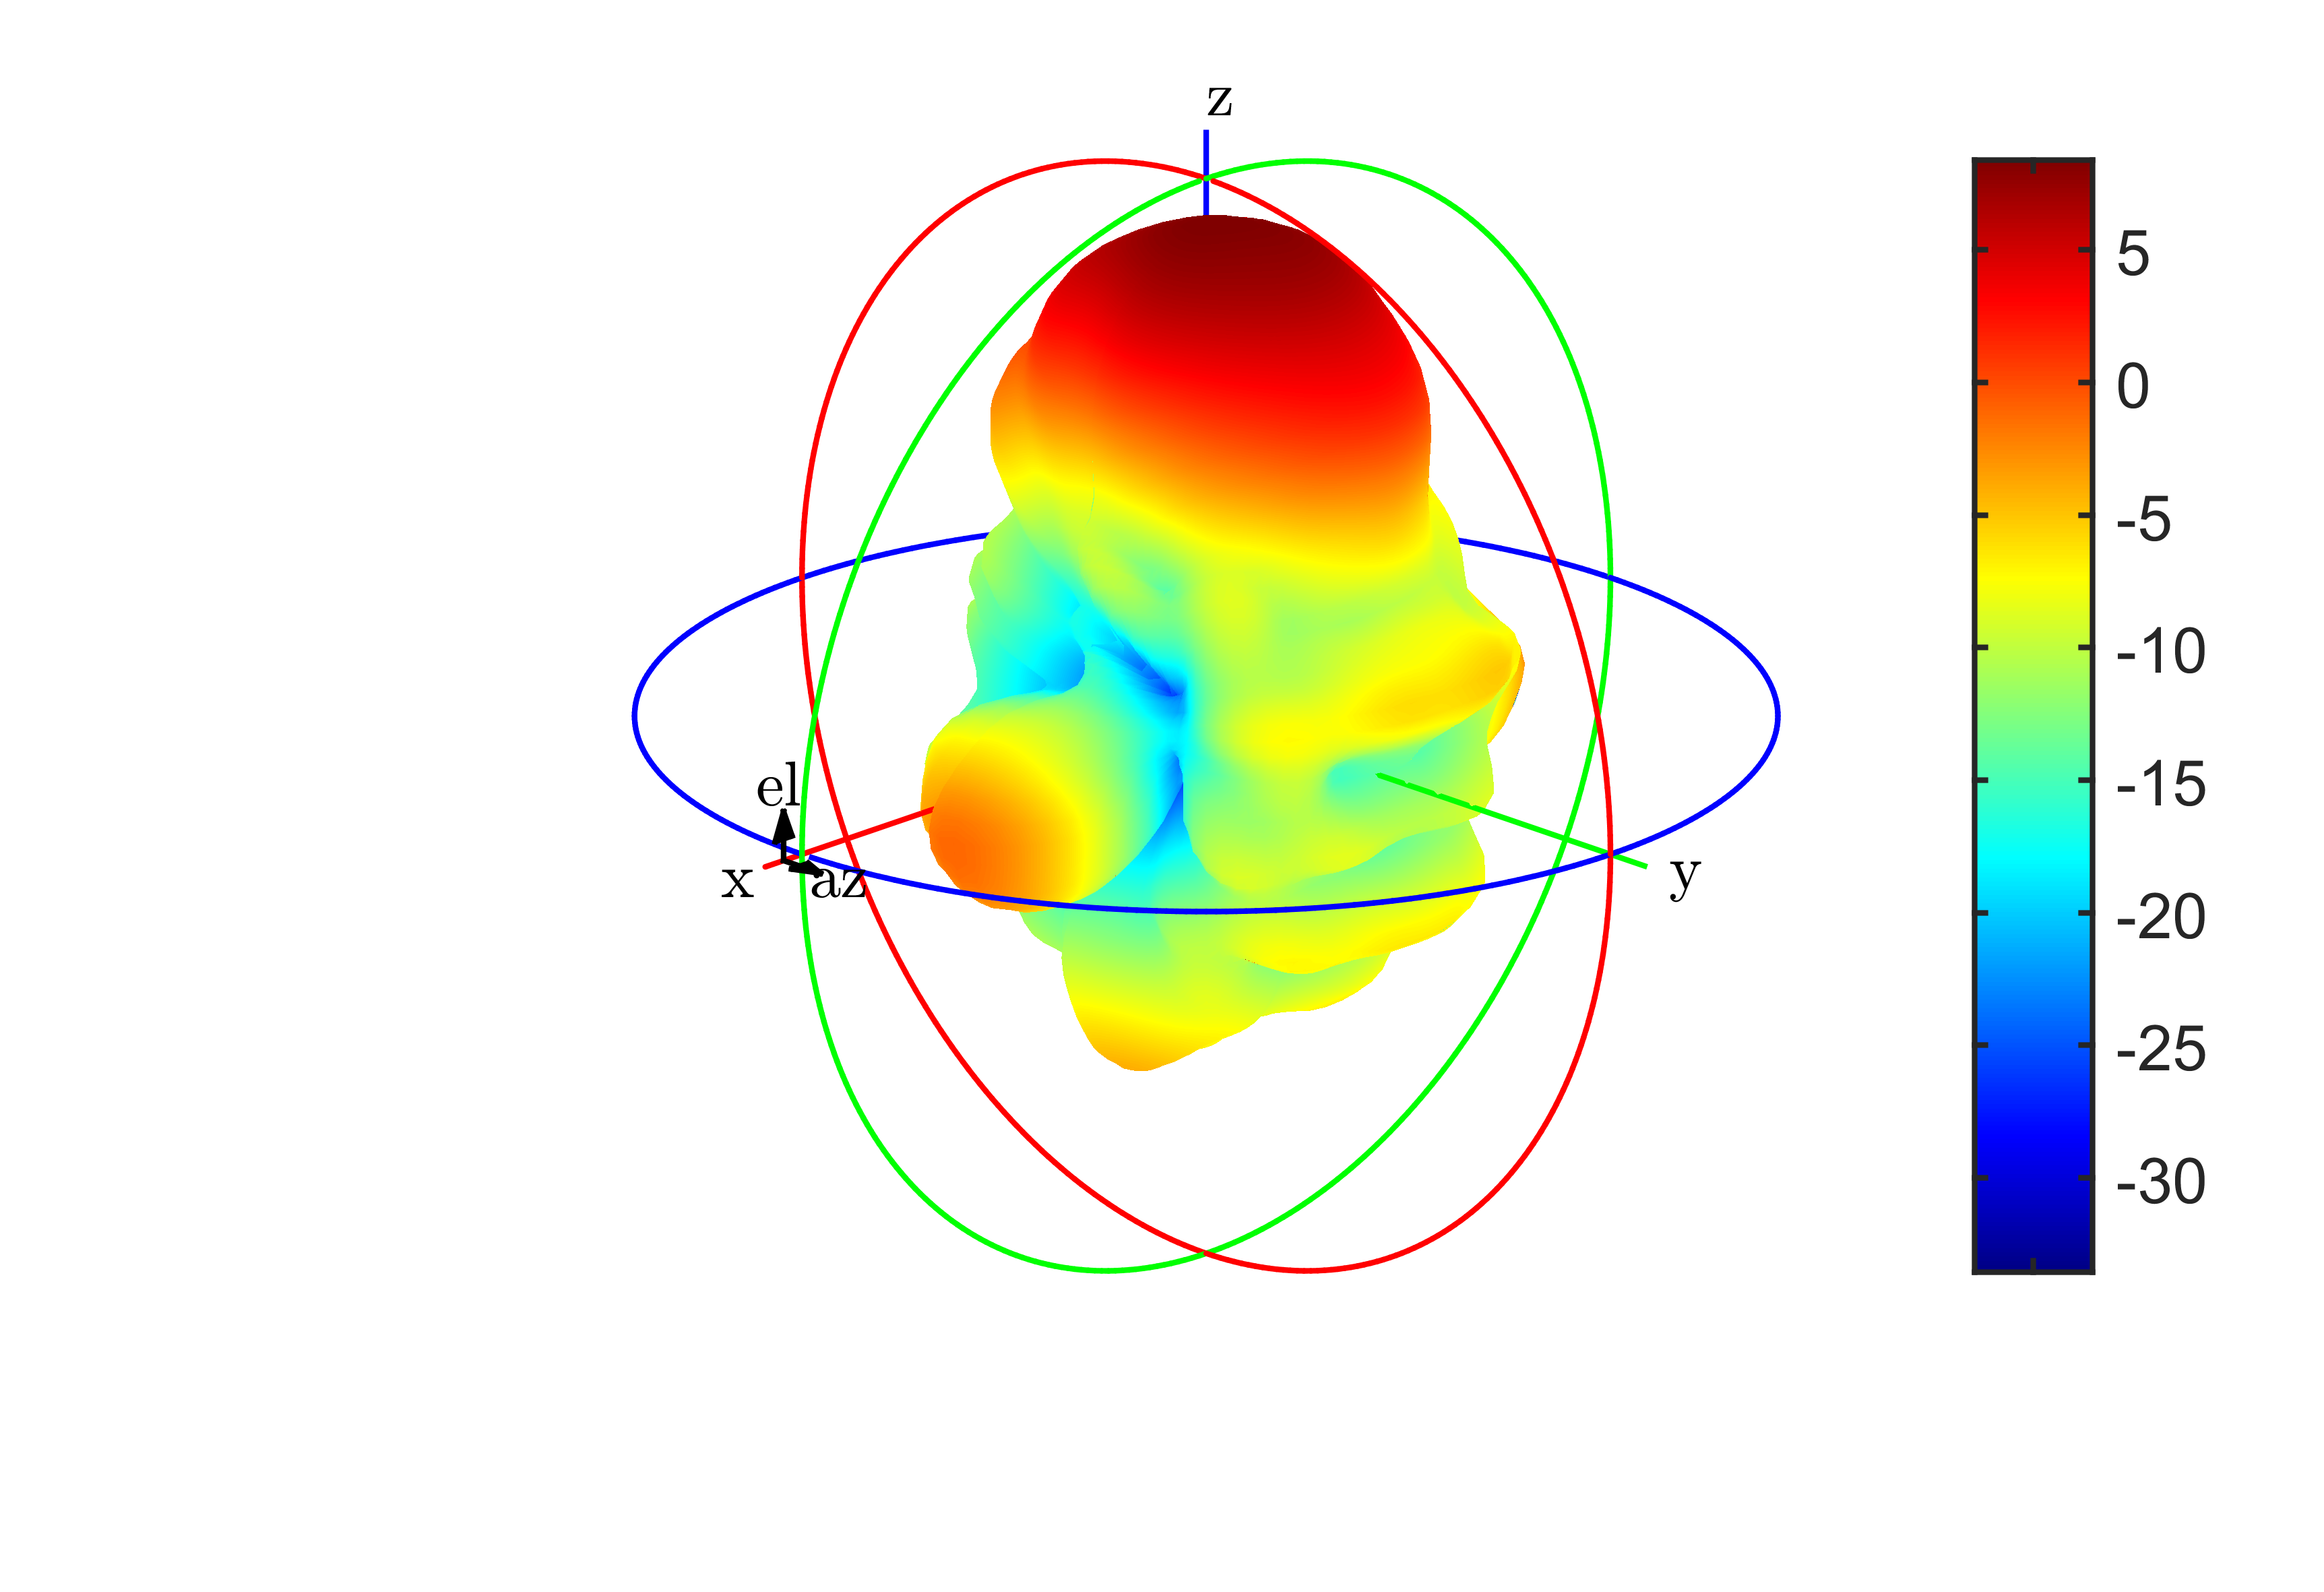
\includegraphics[scale = 0.5]{figures/measurement/antennas/array_2_0p6.png}
\caption{Farfield for $d = 0.6\lambda$. Maximum gain is 8.4dB}
    \label{fig:chamber_two_ant_ff:06}
  \end{minipage}
\end{figure}


\begin{figure}[H]
  \centering
  \begin{minipage}[b]{0.5\textwidth}
	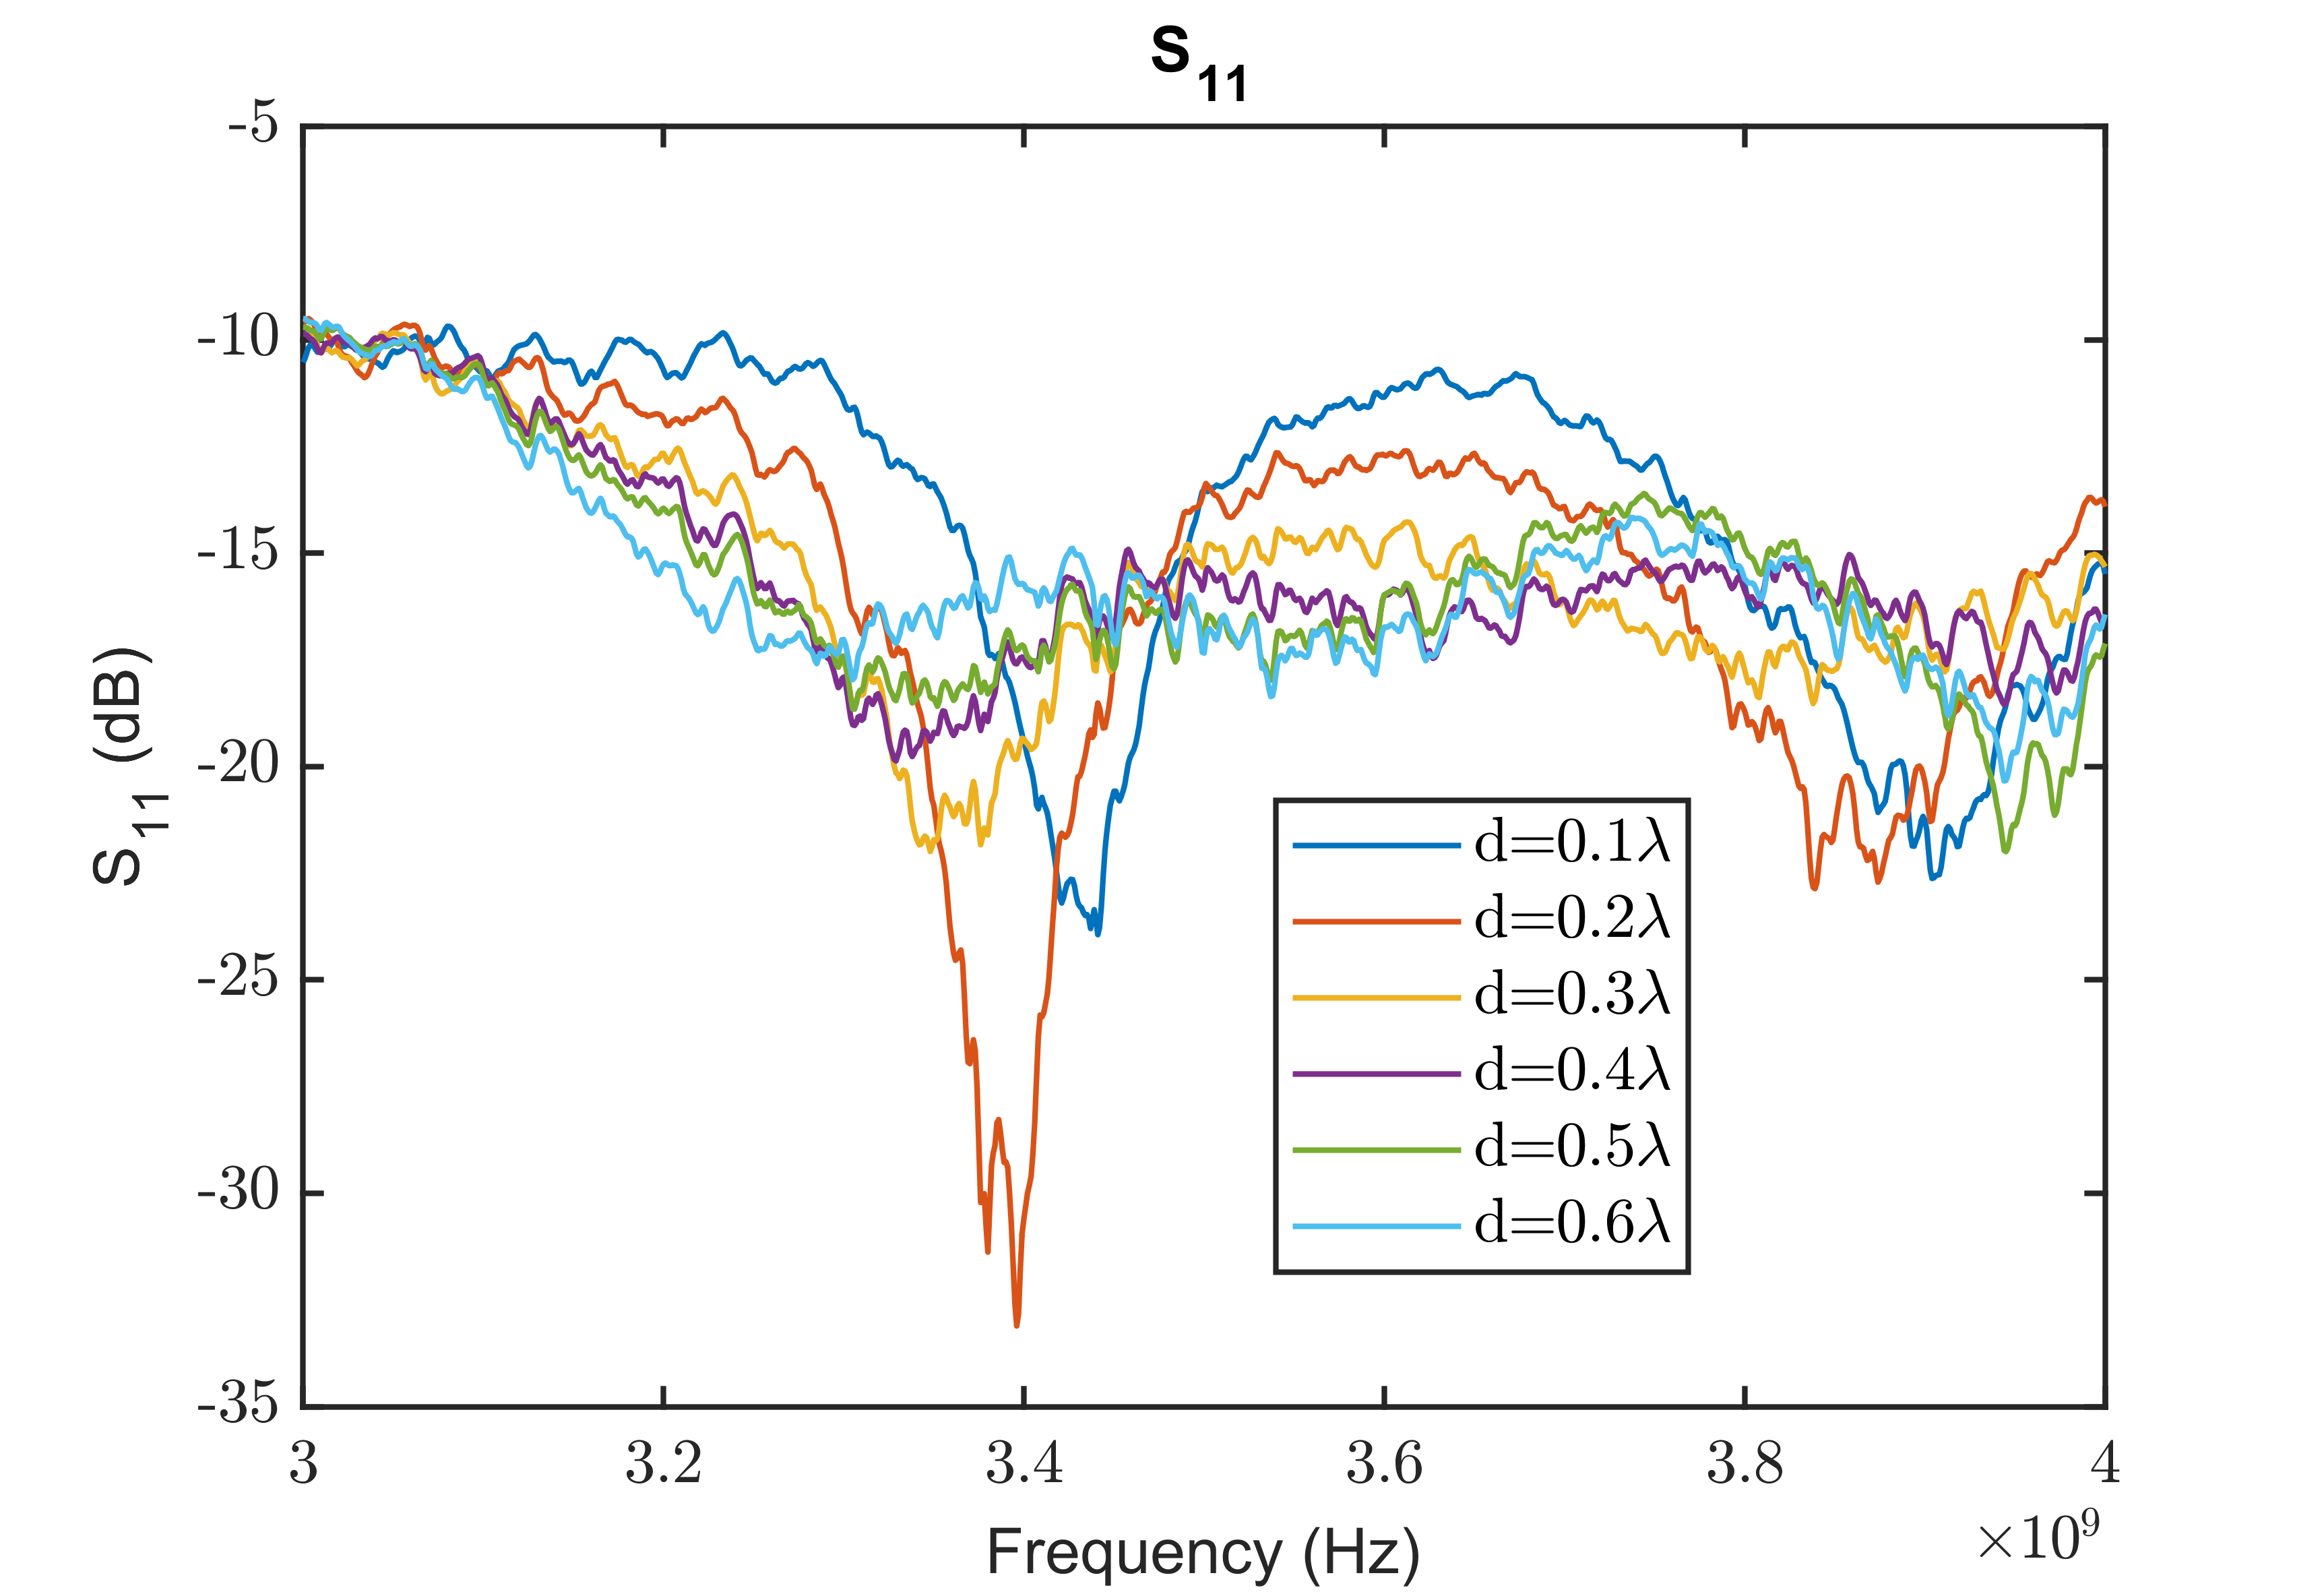
\includegraphics[scale = 0.5]{figures/measurement/antennas/spar_two_ant_s11.png}
	\caption{Measured $S_{11}$ with two antennas}
    \label{fig:chamber_two_ant_s11}
  \end{minipage}
  \hfill
  \begin{minipage}[b]{0.4\textwidth}
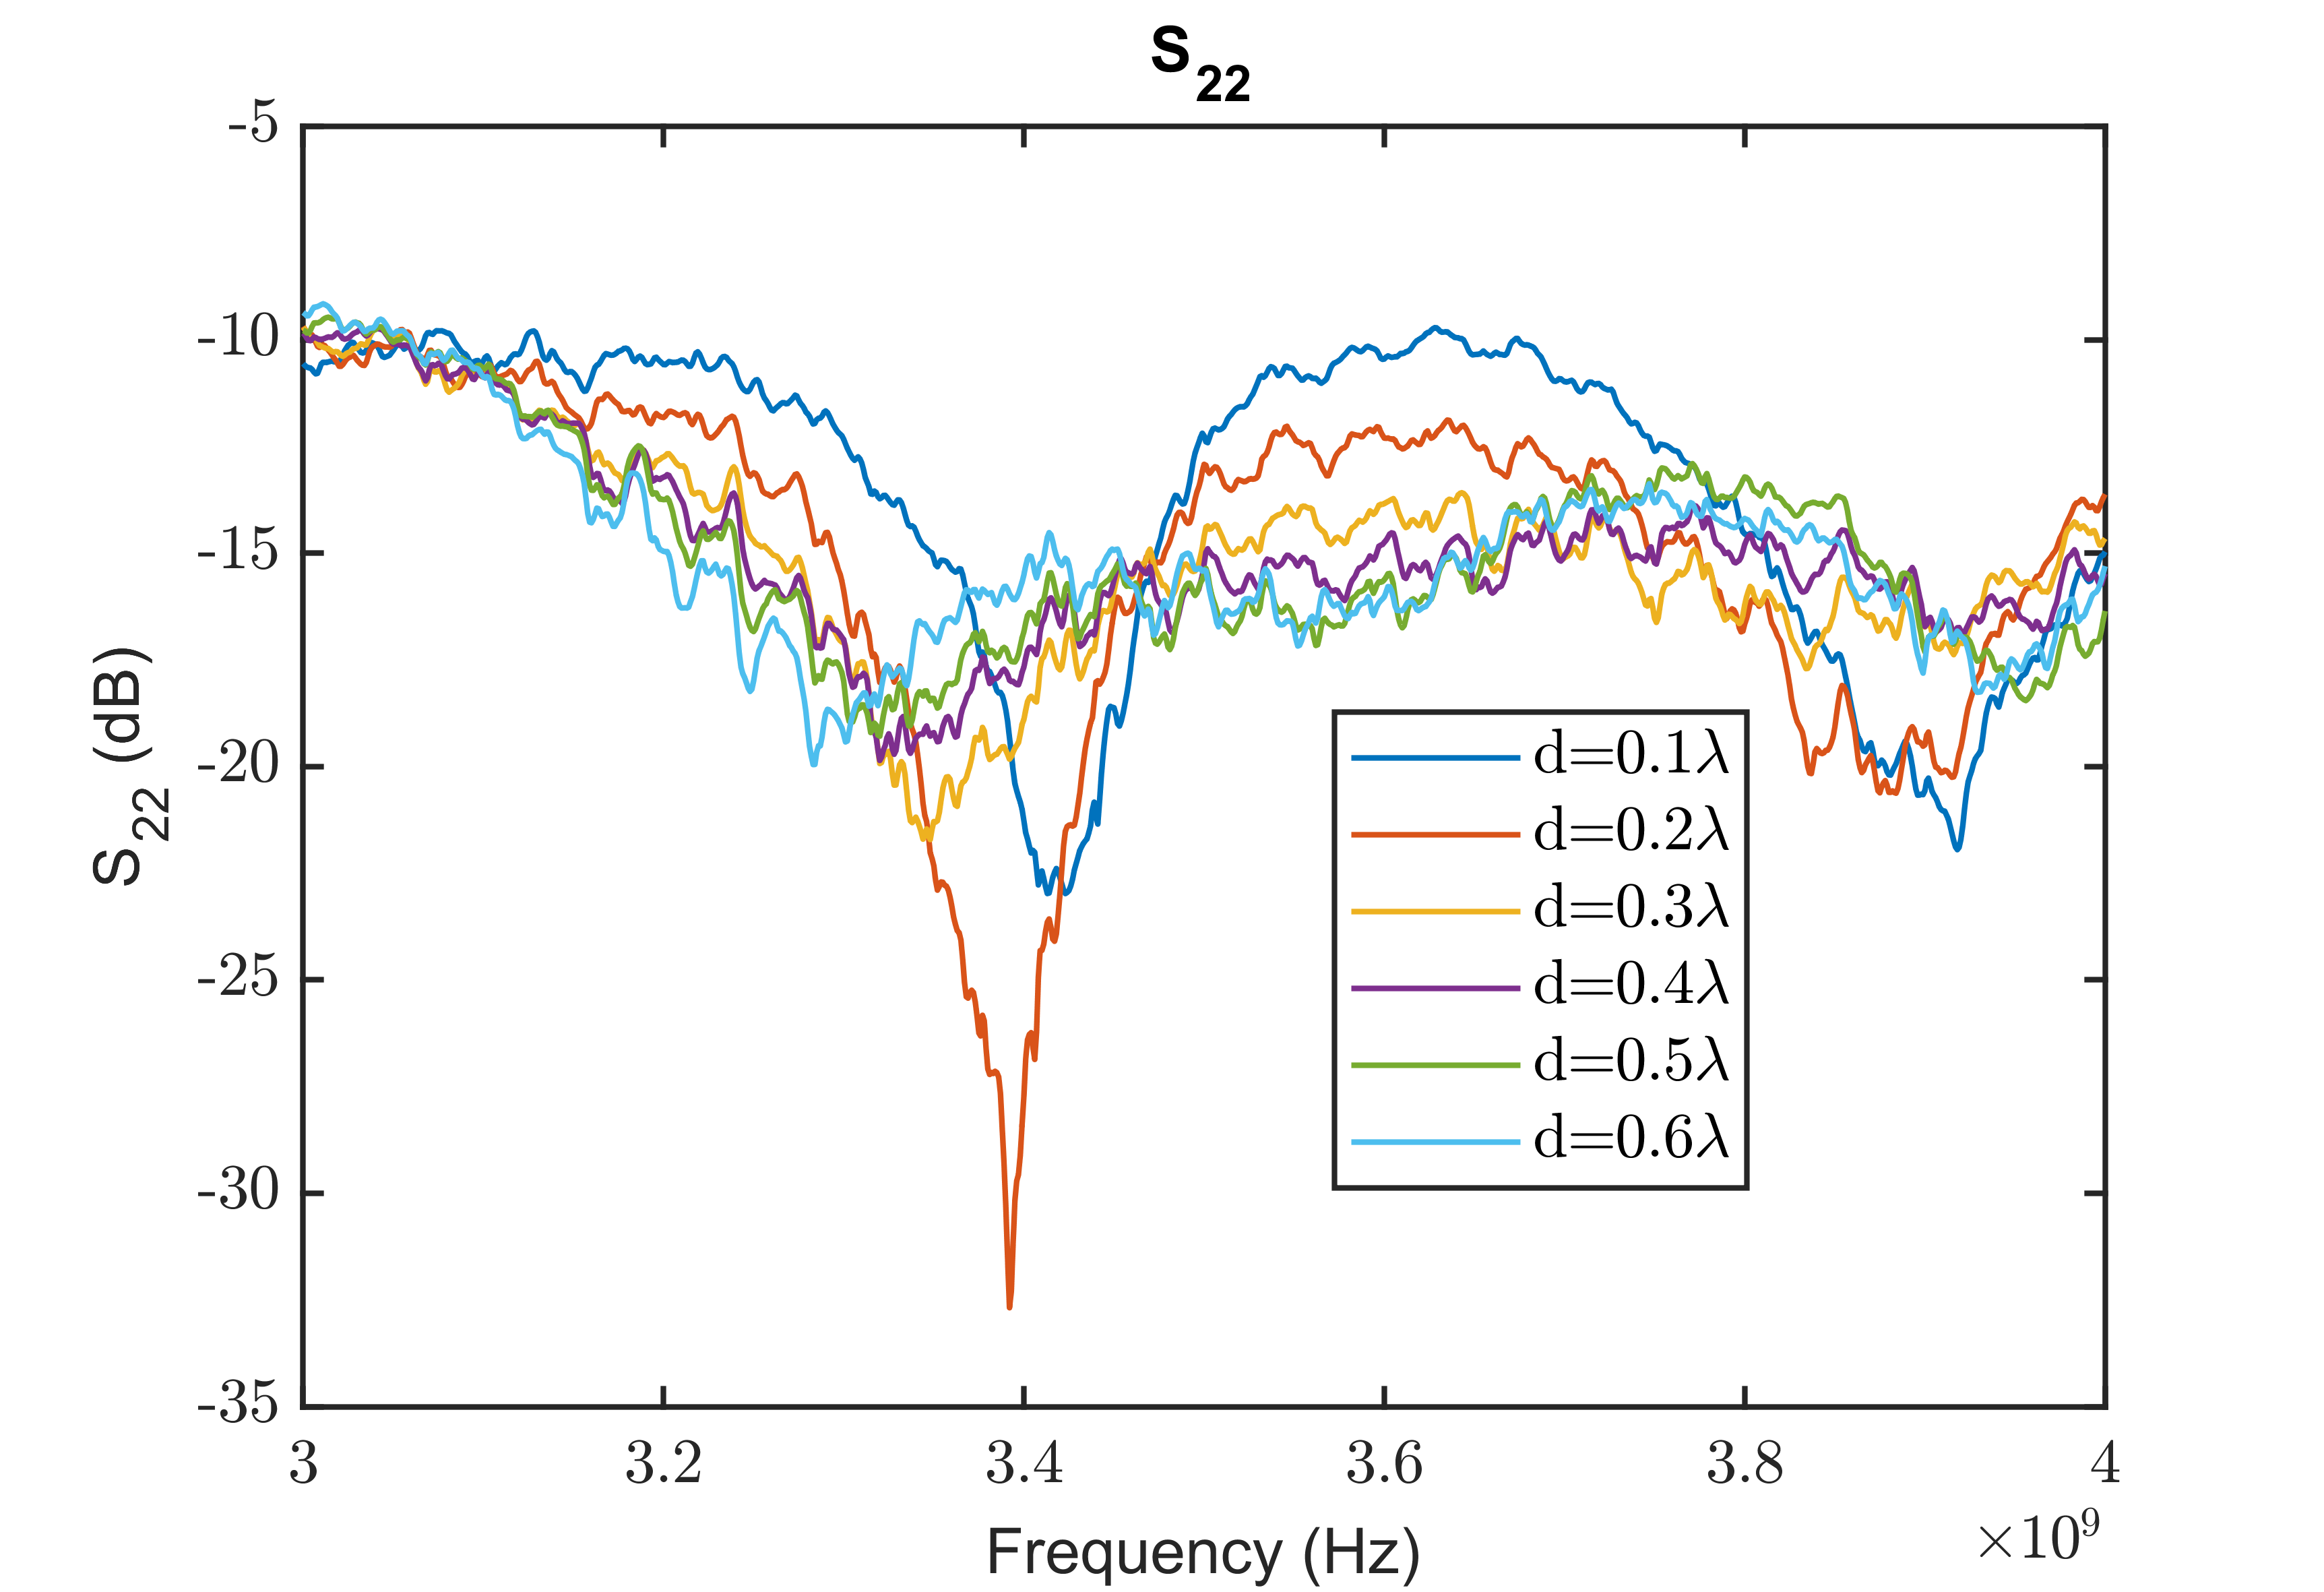
\includegraphics[scale = 0.5]{figures/measurement/antennas/spar_two_ant_s22.png}
\caption{Measured $S_{22}$ with two antennas}
    \label{fig:chamber_two_ant_s22}
  \end{minipage}
\end{figure}

\begin{figure}[H]
  \centering
  \begin{minipage}[b]{0.5\textwidth}
	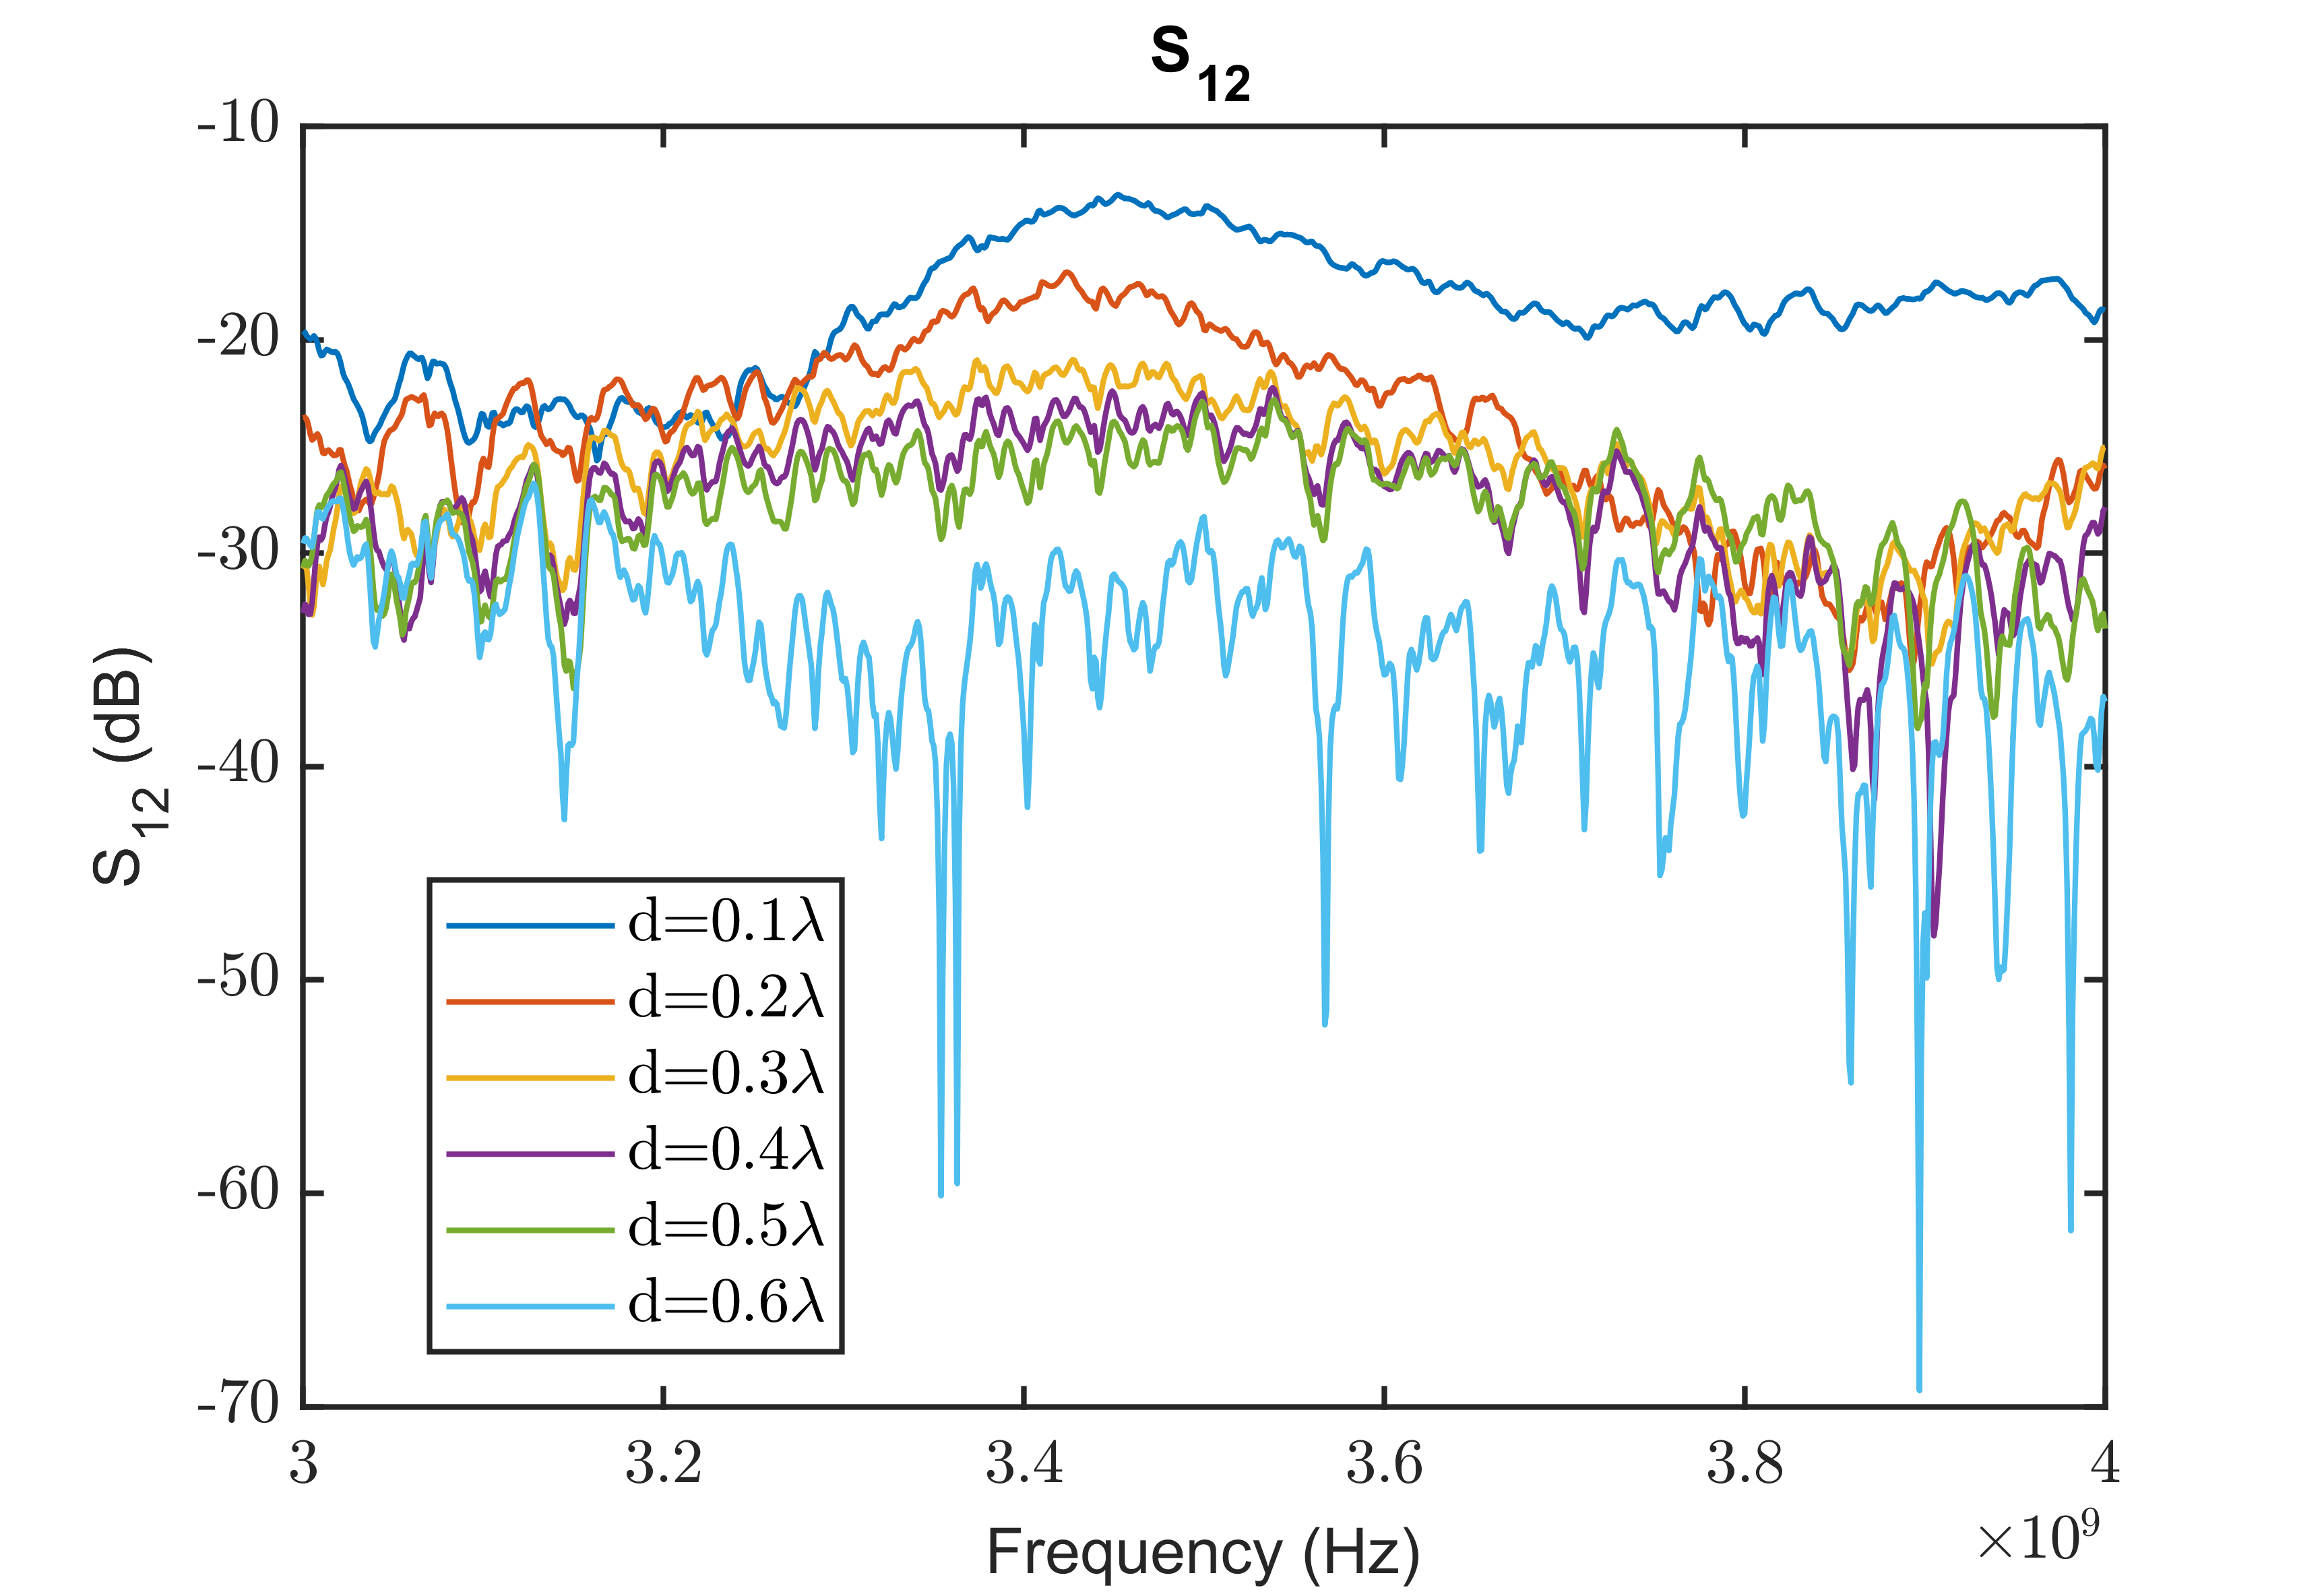
\includegraphics[scale = 0.5]{figures/measurement/antennas/spar_two_ant_s12.png}
	\caption{Measured $S_{12}$ with two antennas}
    \label{fig:chamber_two_ant_s12}
  \end{minipage}
  \hfill
  \begin{minipage}[b]{0.4\textwidth}
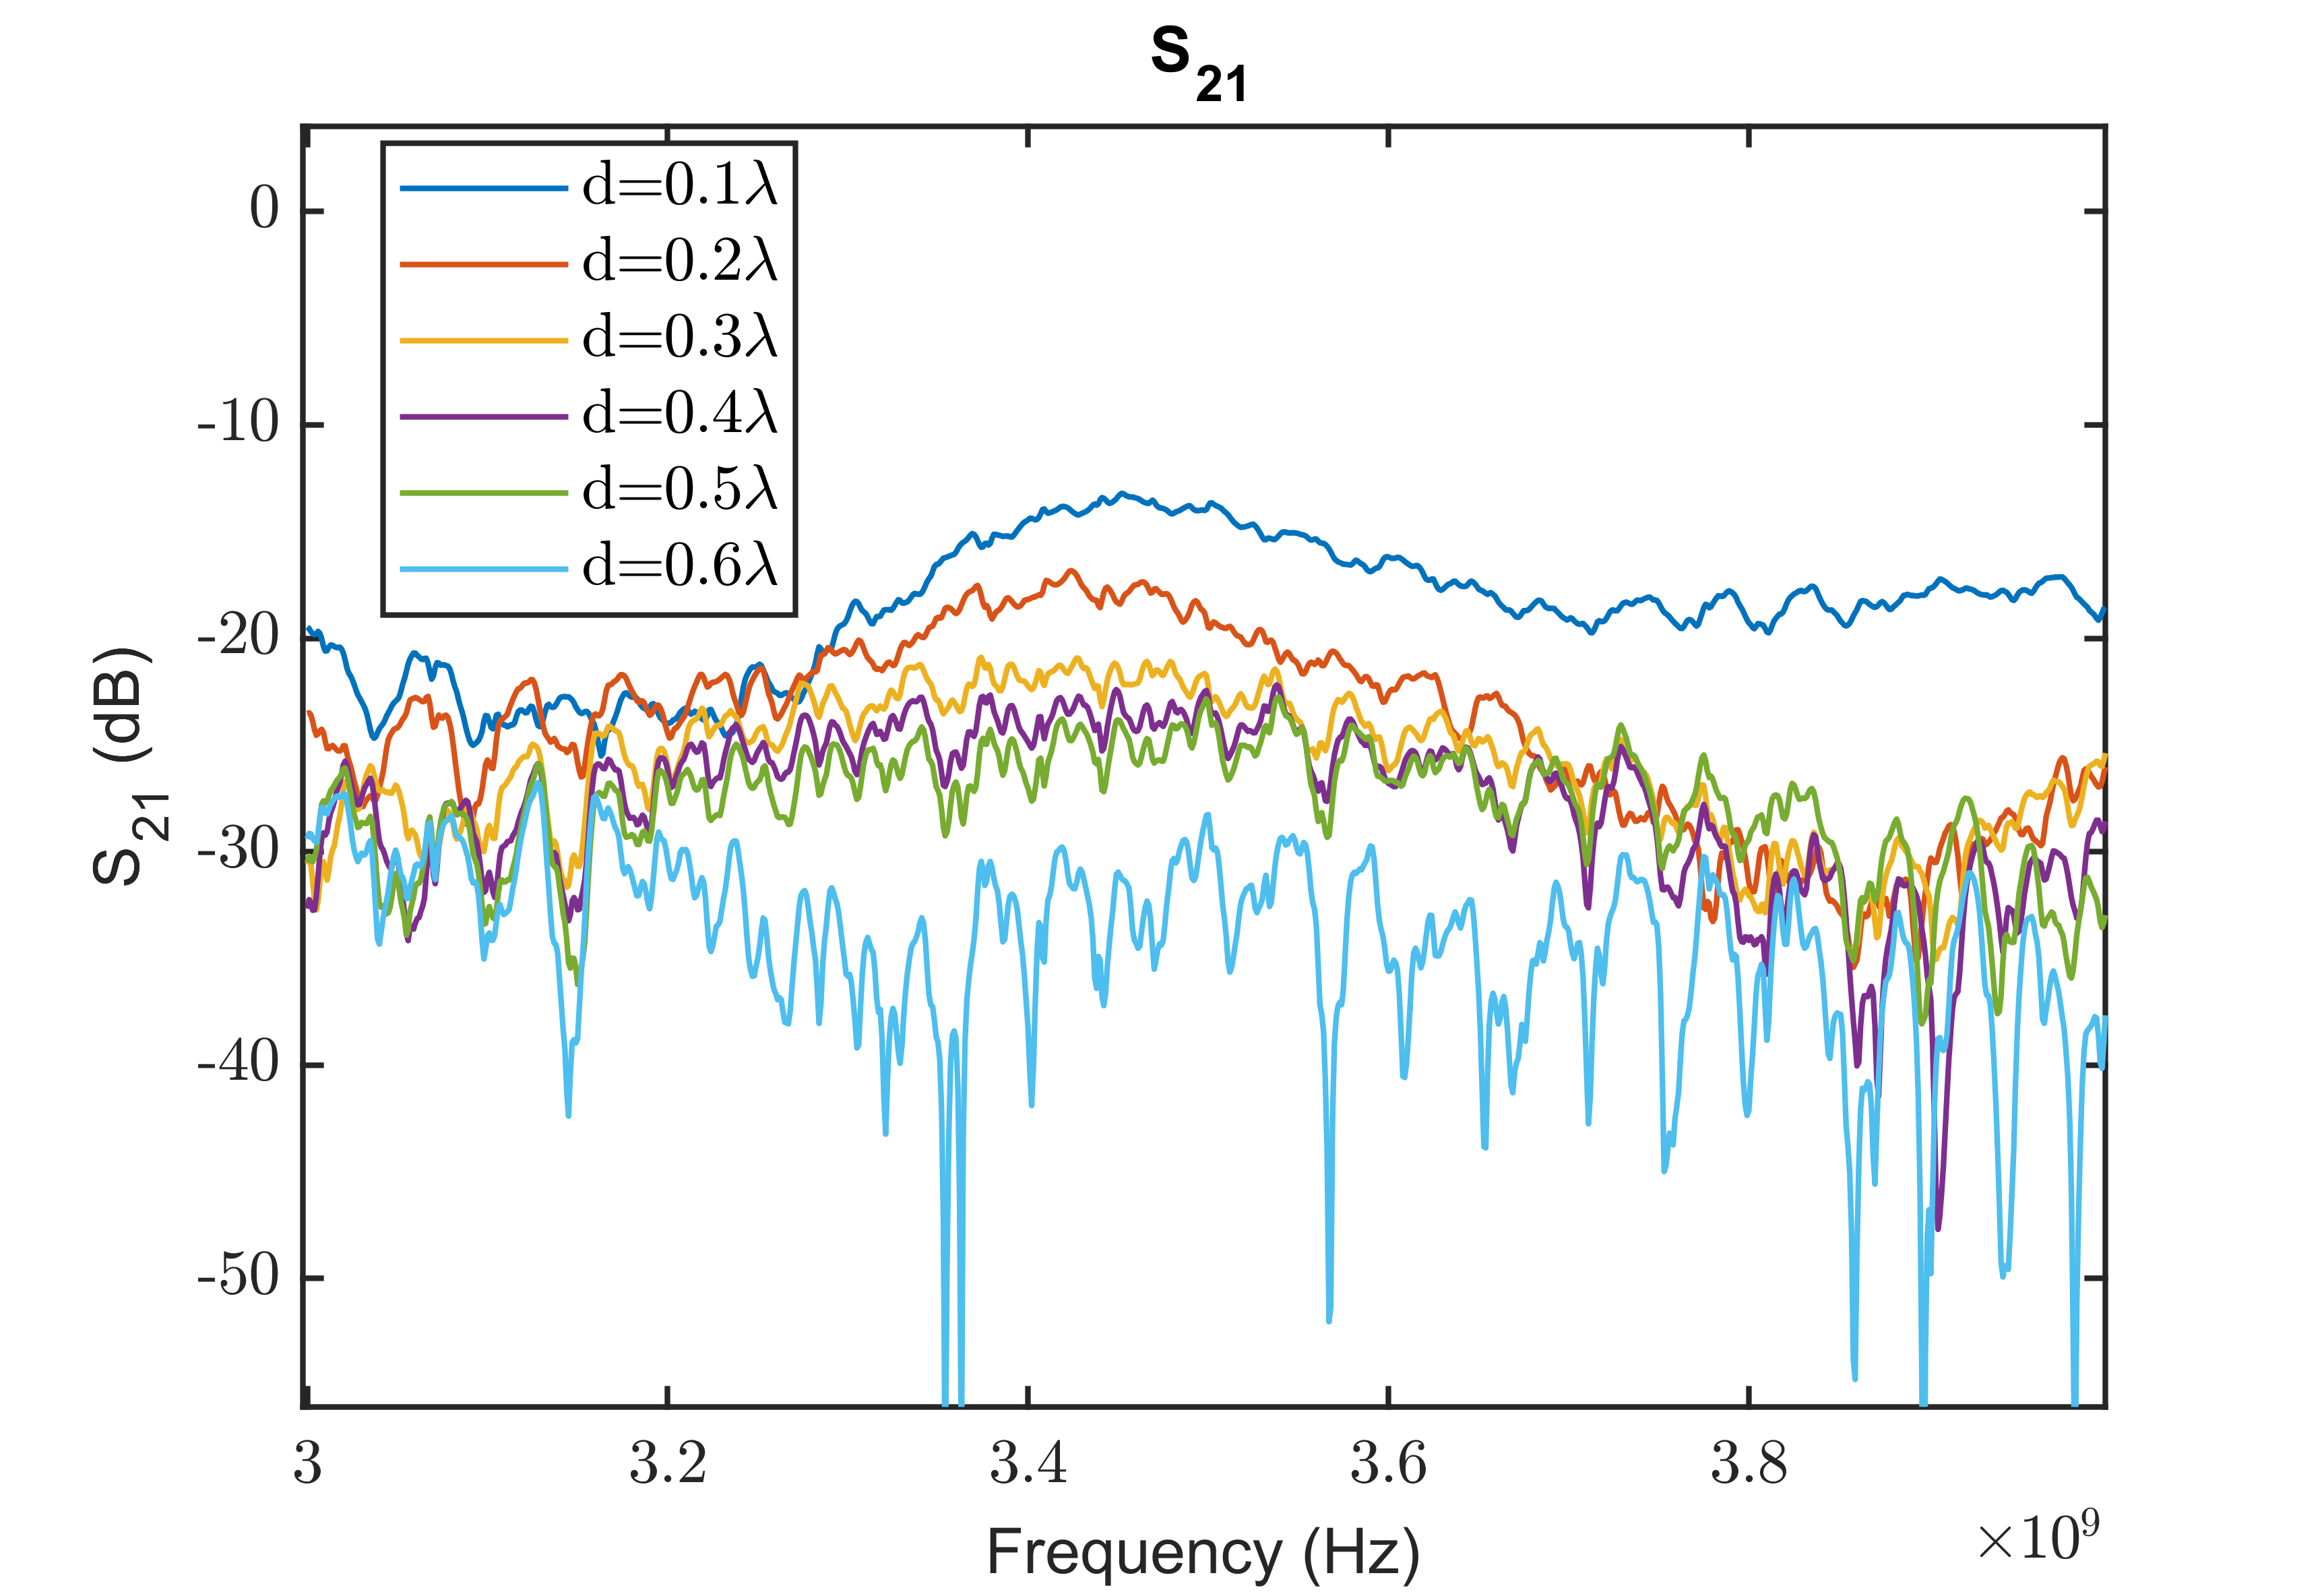
\includegraphics[scale = 0.5]{figures/measurement/antennas/spar_two_ant_s21.png}
\caption{Measured $S_{21}$ with two antennas}
    \label{fig:chamber_two_ant_s21}
  \end{minipage}
\end{figure}


%%%%%%%%%%%%%%%%%%%%%%%%%%%%%%%%%%%%%%%%%%%%%%%%%%%%%%%%%%%%%%%%%%%%%%%%%%%%%%%%%%%%%%%%%%%%%%%%%%%%%%%%%%%%%%%%%
\section{Four antennas}
In this section four antennas is measured. The expected gain is the same as for one antenna because of the powerdivider. Like the case for the measurement done at two antennas the distances is also varied in these measurements. The unused antennas are terminated to $50\Omega$. It is seen that the farfield flattens even more at this configuration in the y axis. This is mainly caused by the geometry of the antennas. The gain is also higher then expected which can be seen from figure \ref{fig:chamber_four_ant_ff_01} to \ref{fig:chamber_four_ant_ff:06}. The S-parameters are presented in figure  \ref{fig:chamber_four_ant_s11} to \ref{fig:chamber_four_ant_s32}. The S-parameters shows that $S_{11}$ and $S_{44}$ are similar and that $S_{22}$ and $S_{33}$ are similar thou variations is seen. This is mainly because that the distance between the antennas are not exactly the same ant that the antennas in them self have small variations. Like in the case with two antennas the coupling gets worse with a smaller distance ant the return loss also variates a lot. 

\begin{figure}[H]
\centering 
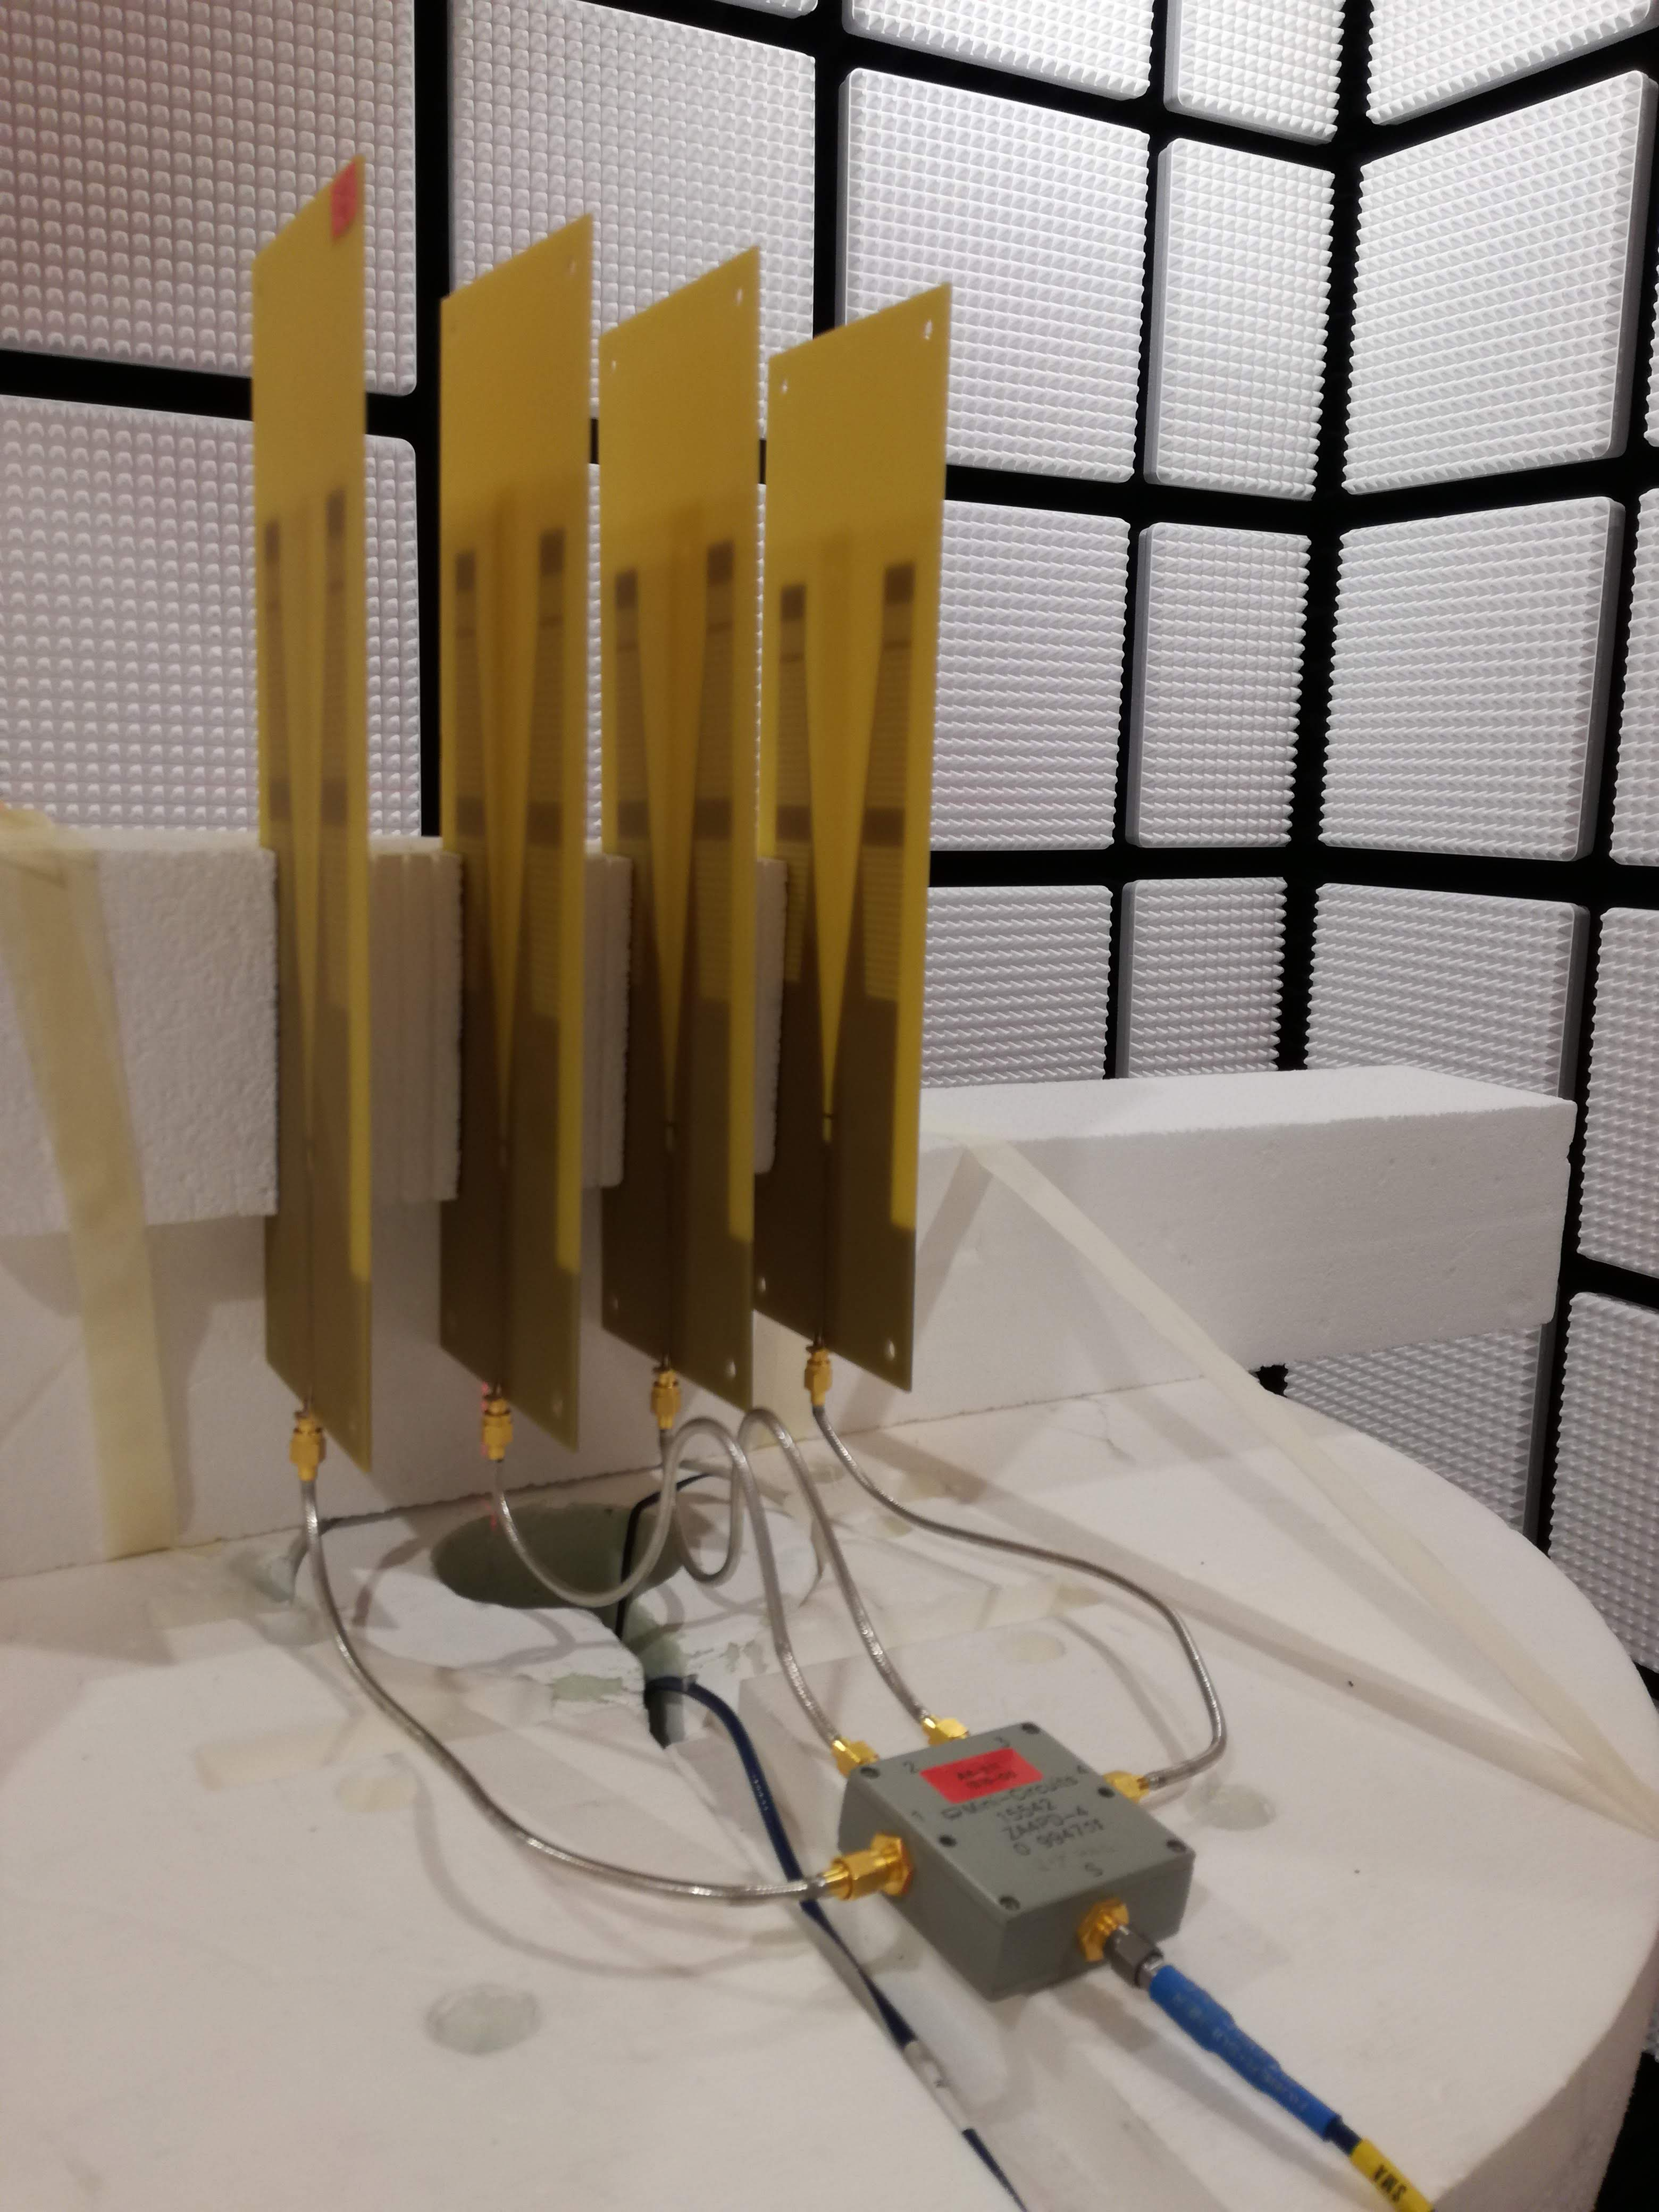
\includegraphics[scale = 0.05]{figures/measurement/antennas/four_ant.jpg}
\caption{Measurement of four antennas with a powerdivider in an anechoic chamber. The distances between the antennas are varied for every measurement. The distance is $0.5\lambda$ on the picture}
\label{fig:chamber_four_ant}
\end{figure} 


\begin{figure}[H]
  \centering
  \begin{minipage}[b]{0.5\textwidth}
	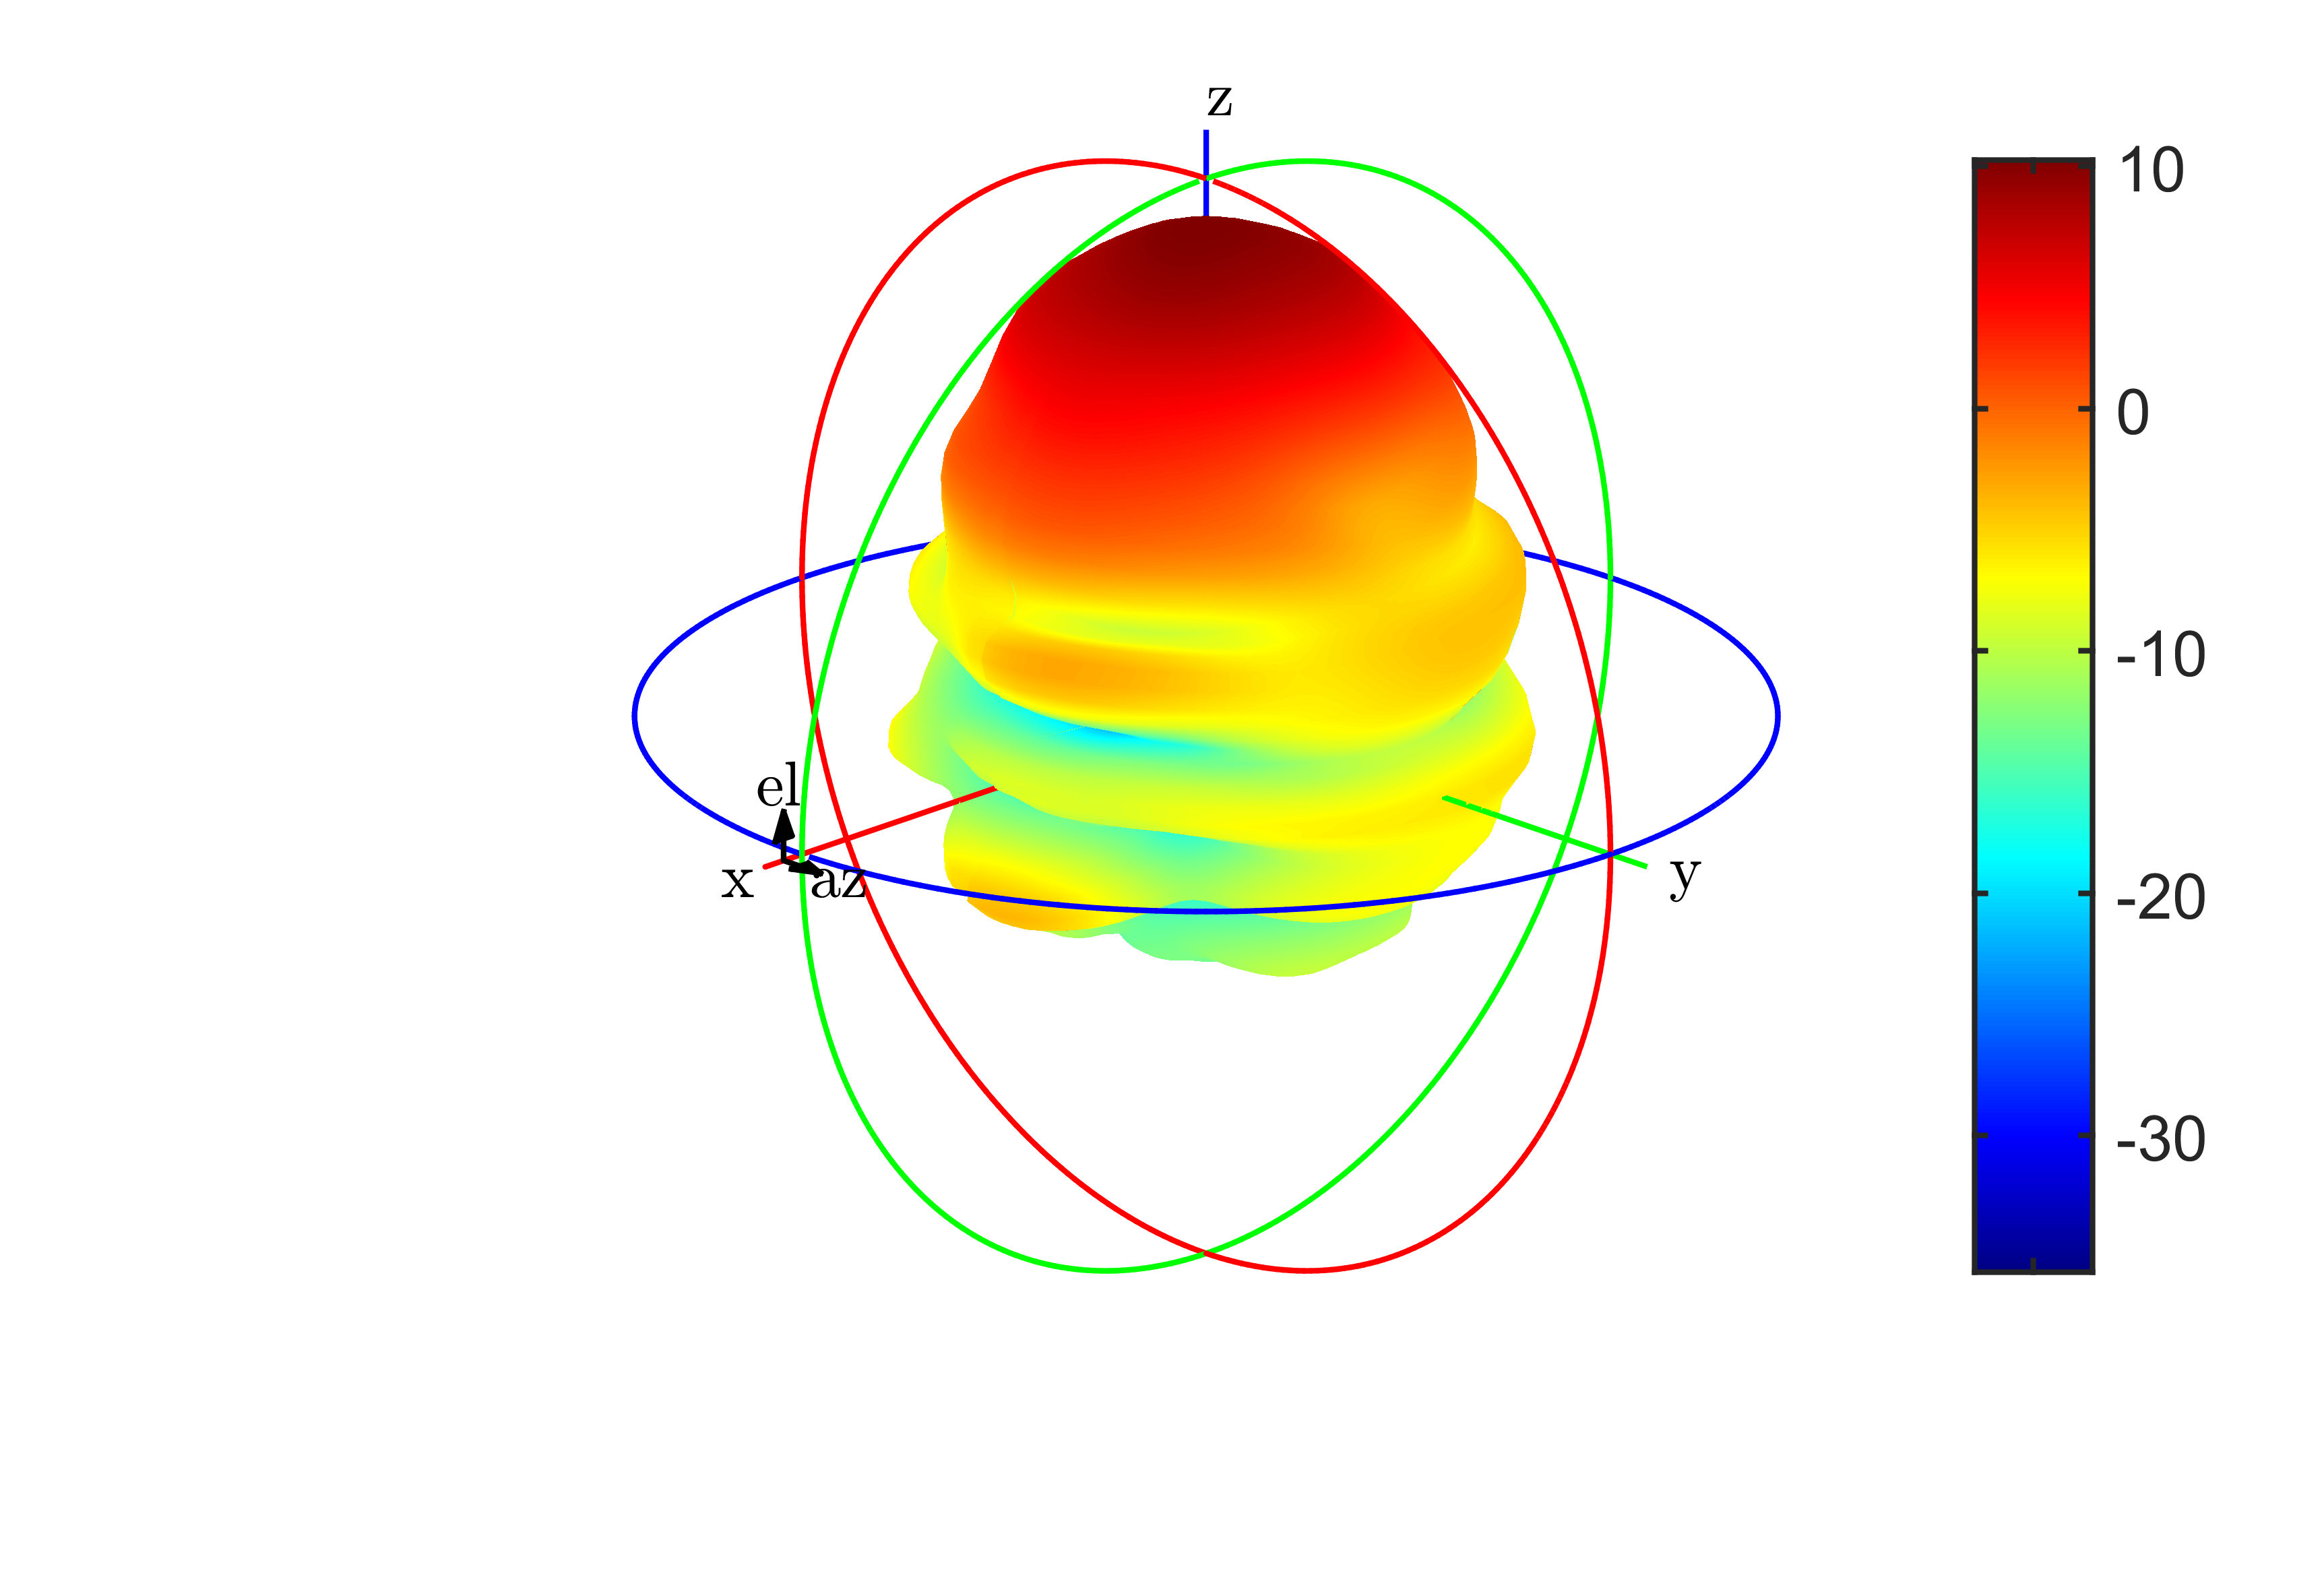
\includegraphics[scale = 0.5]{figures/measurement/antennas/array_4_0p1.png}
	\caption{Farfield for $d = 0.1\lambda$. Maximum gain is 10.3dB}
    \label{fig:chamber_four_ant_ff_01}
  \end{minipage}
  \hfill
  \begin{minipage}[b]{0.4\textwidth}
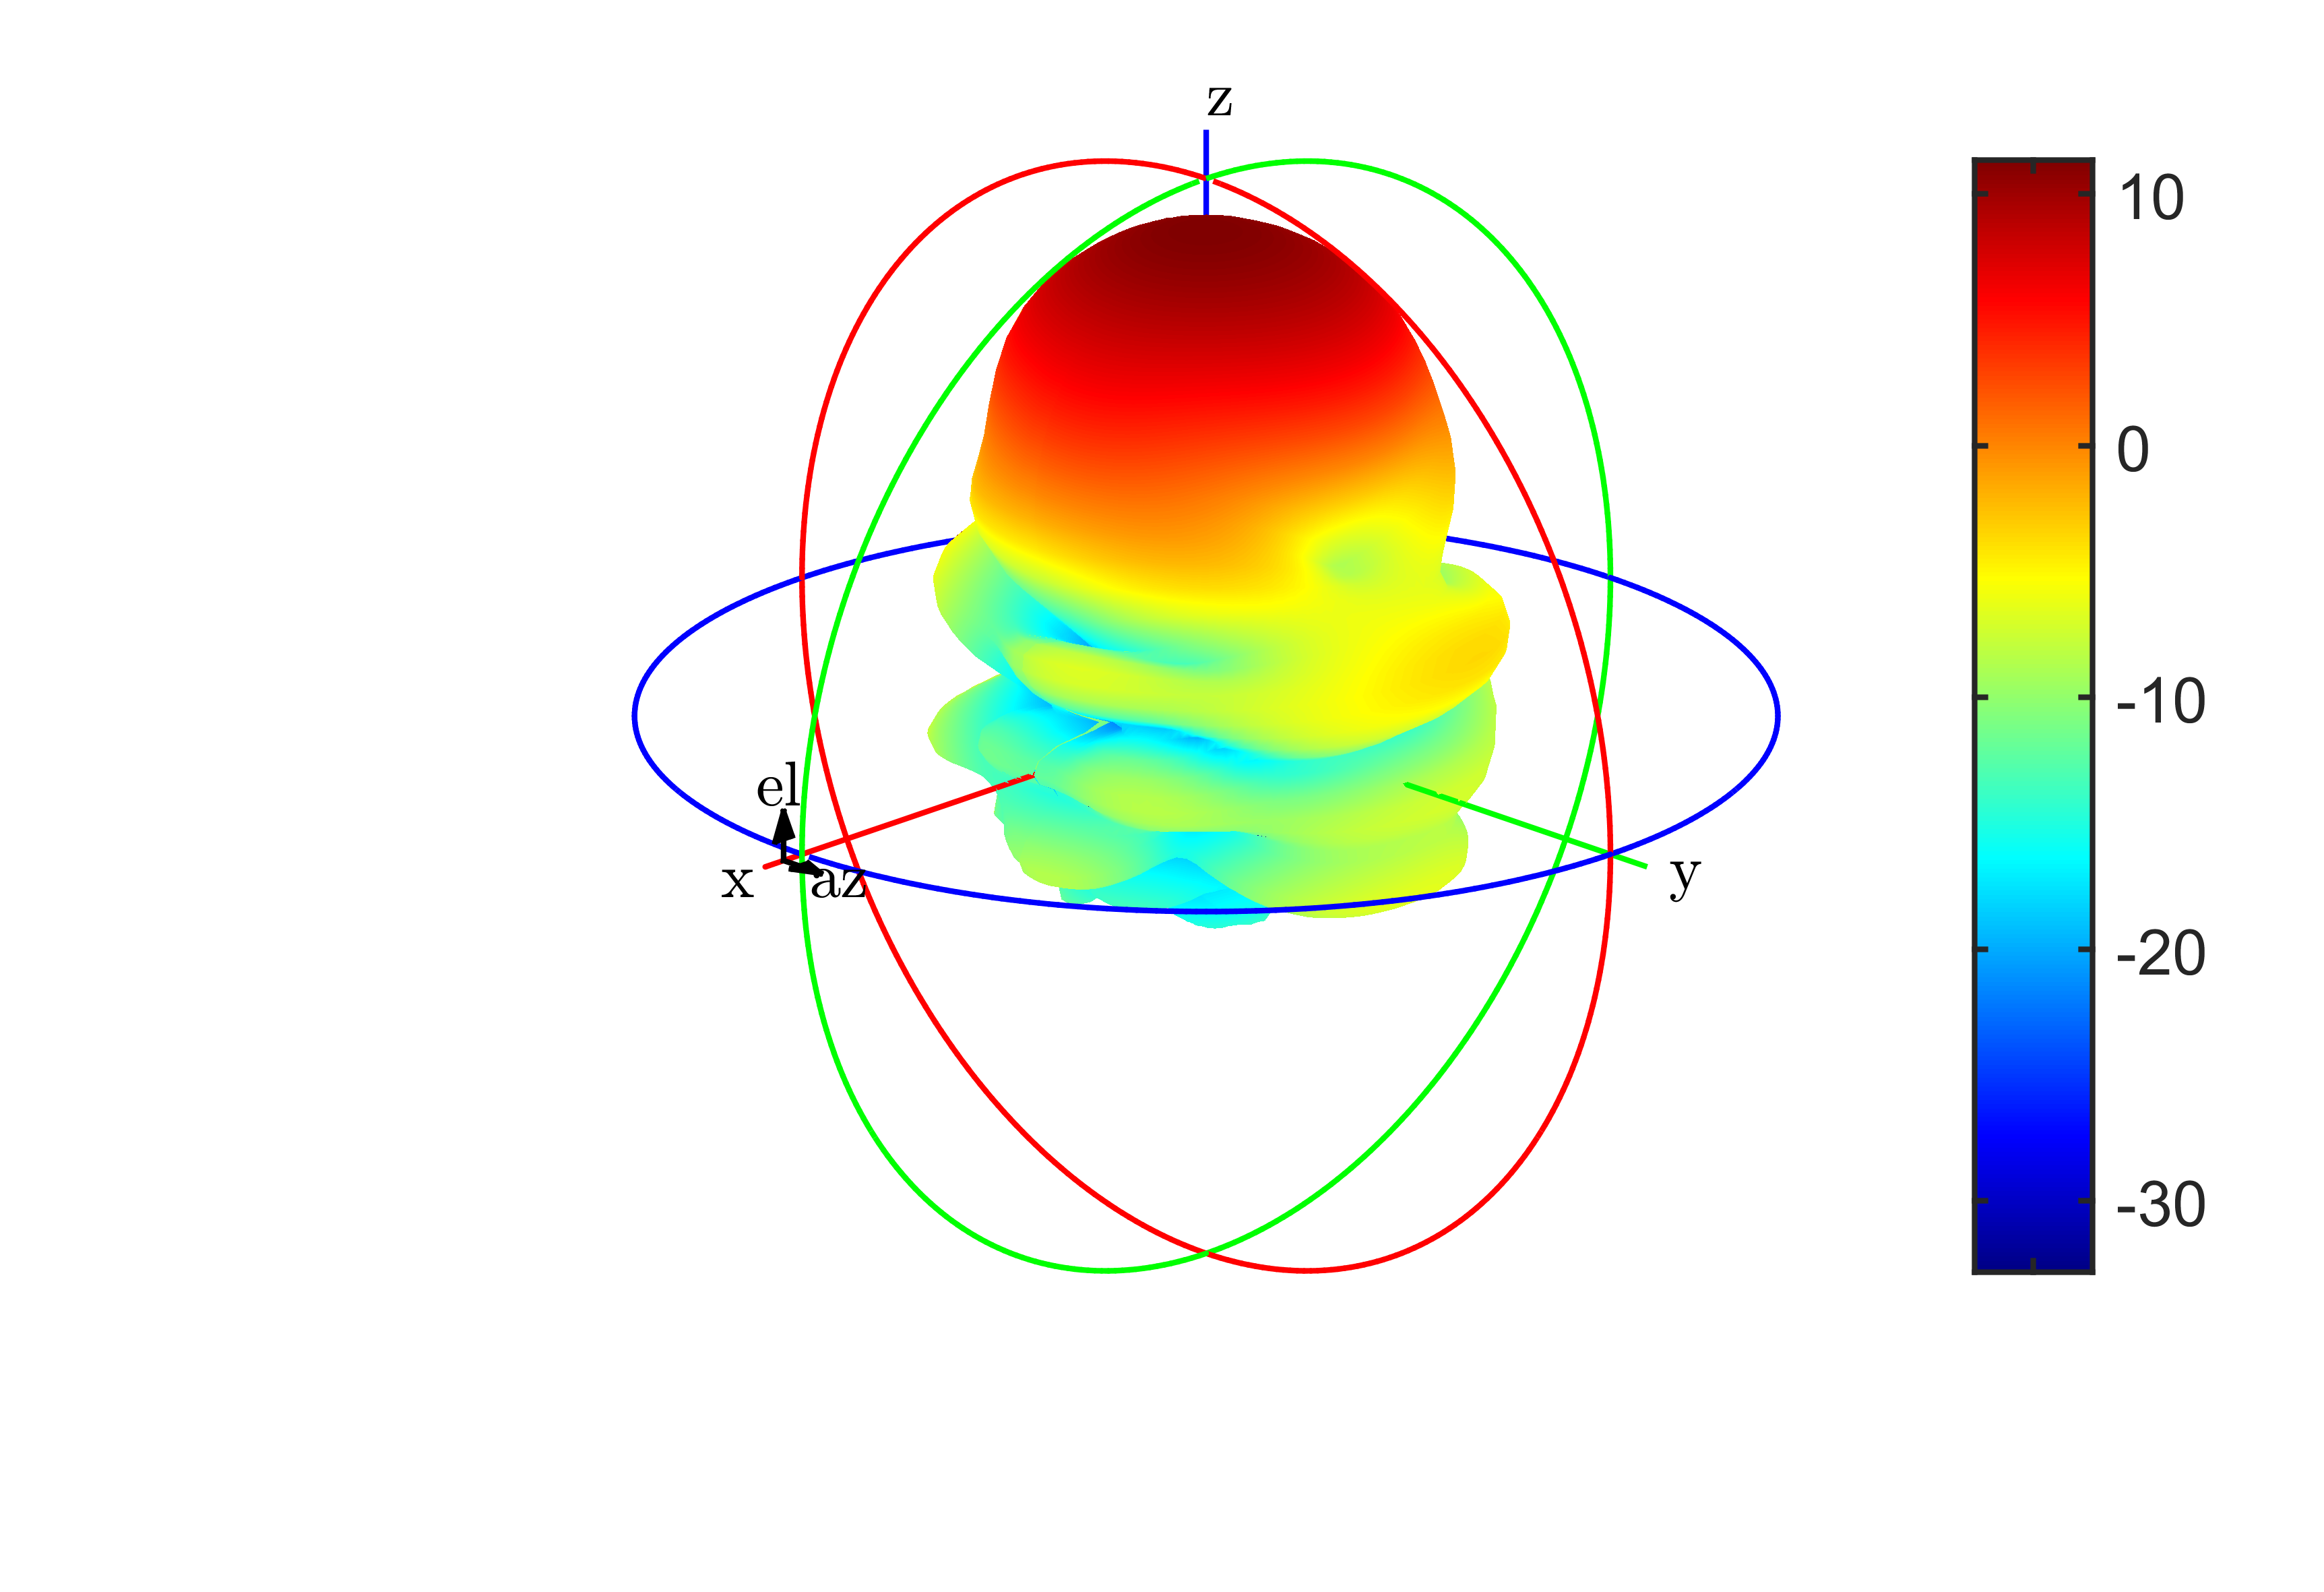
\includegraphics[scale = 0.5]{figures/measurement/antennas/array_4_0p2.png}
\caption{Farfield for $d = 0.2\lambda$. Maximum gain is 11.3dB}
    \label{fig:chamber_four_ant_ff:02}
  \end{minipage}
\end{figure}

\begin{figure}[H]
  \centering
  \begin{minipage}[b]{0.5\textwidth}
	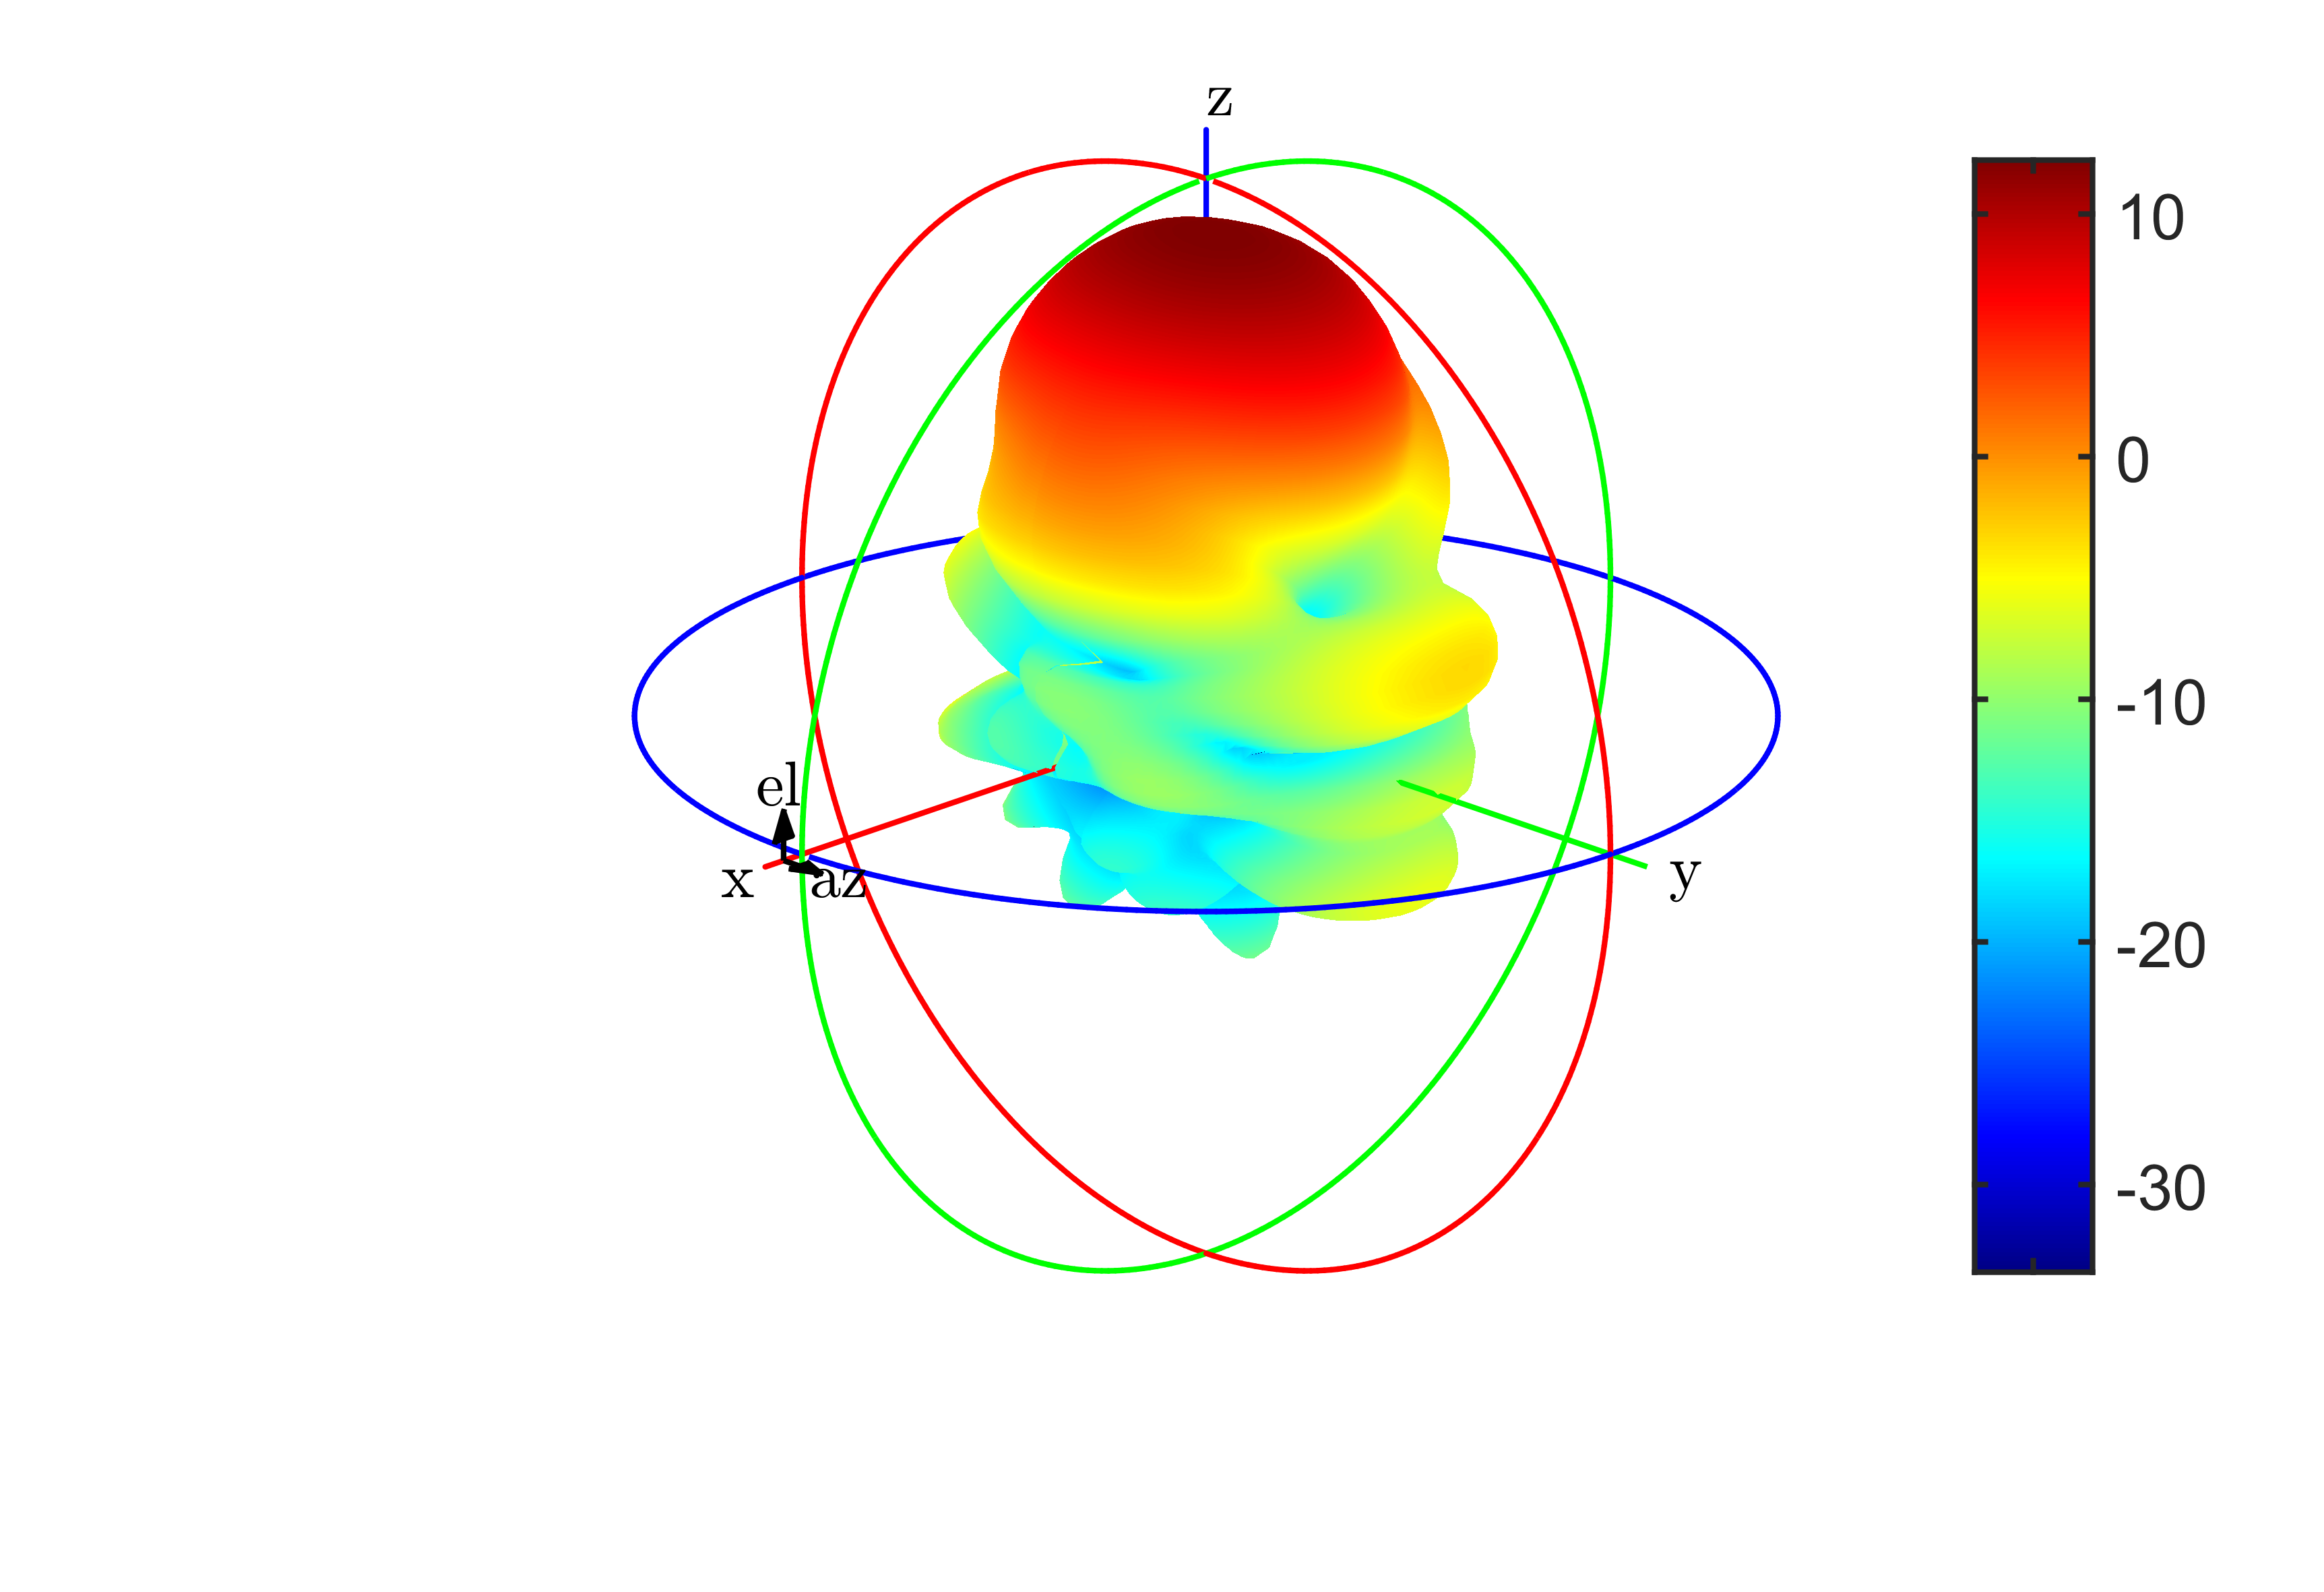
\includegraphics[scale = 0.5]{figures/measurement/antennas/array_4_0p3.png}
	\caption{Farfield for $d = 0.3\lambda$. Maximum gain is 12.2dB}
    \label{fig:chamber_four_ant_ff_03}
  \end{minipage}
  \hfill
  \begin{minipage}[b]{0.4\textwidth}
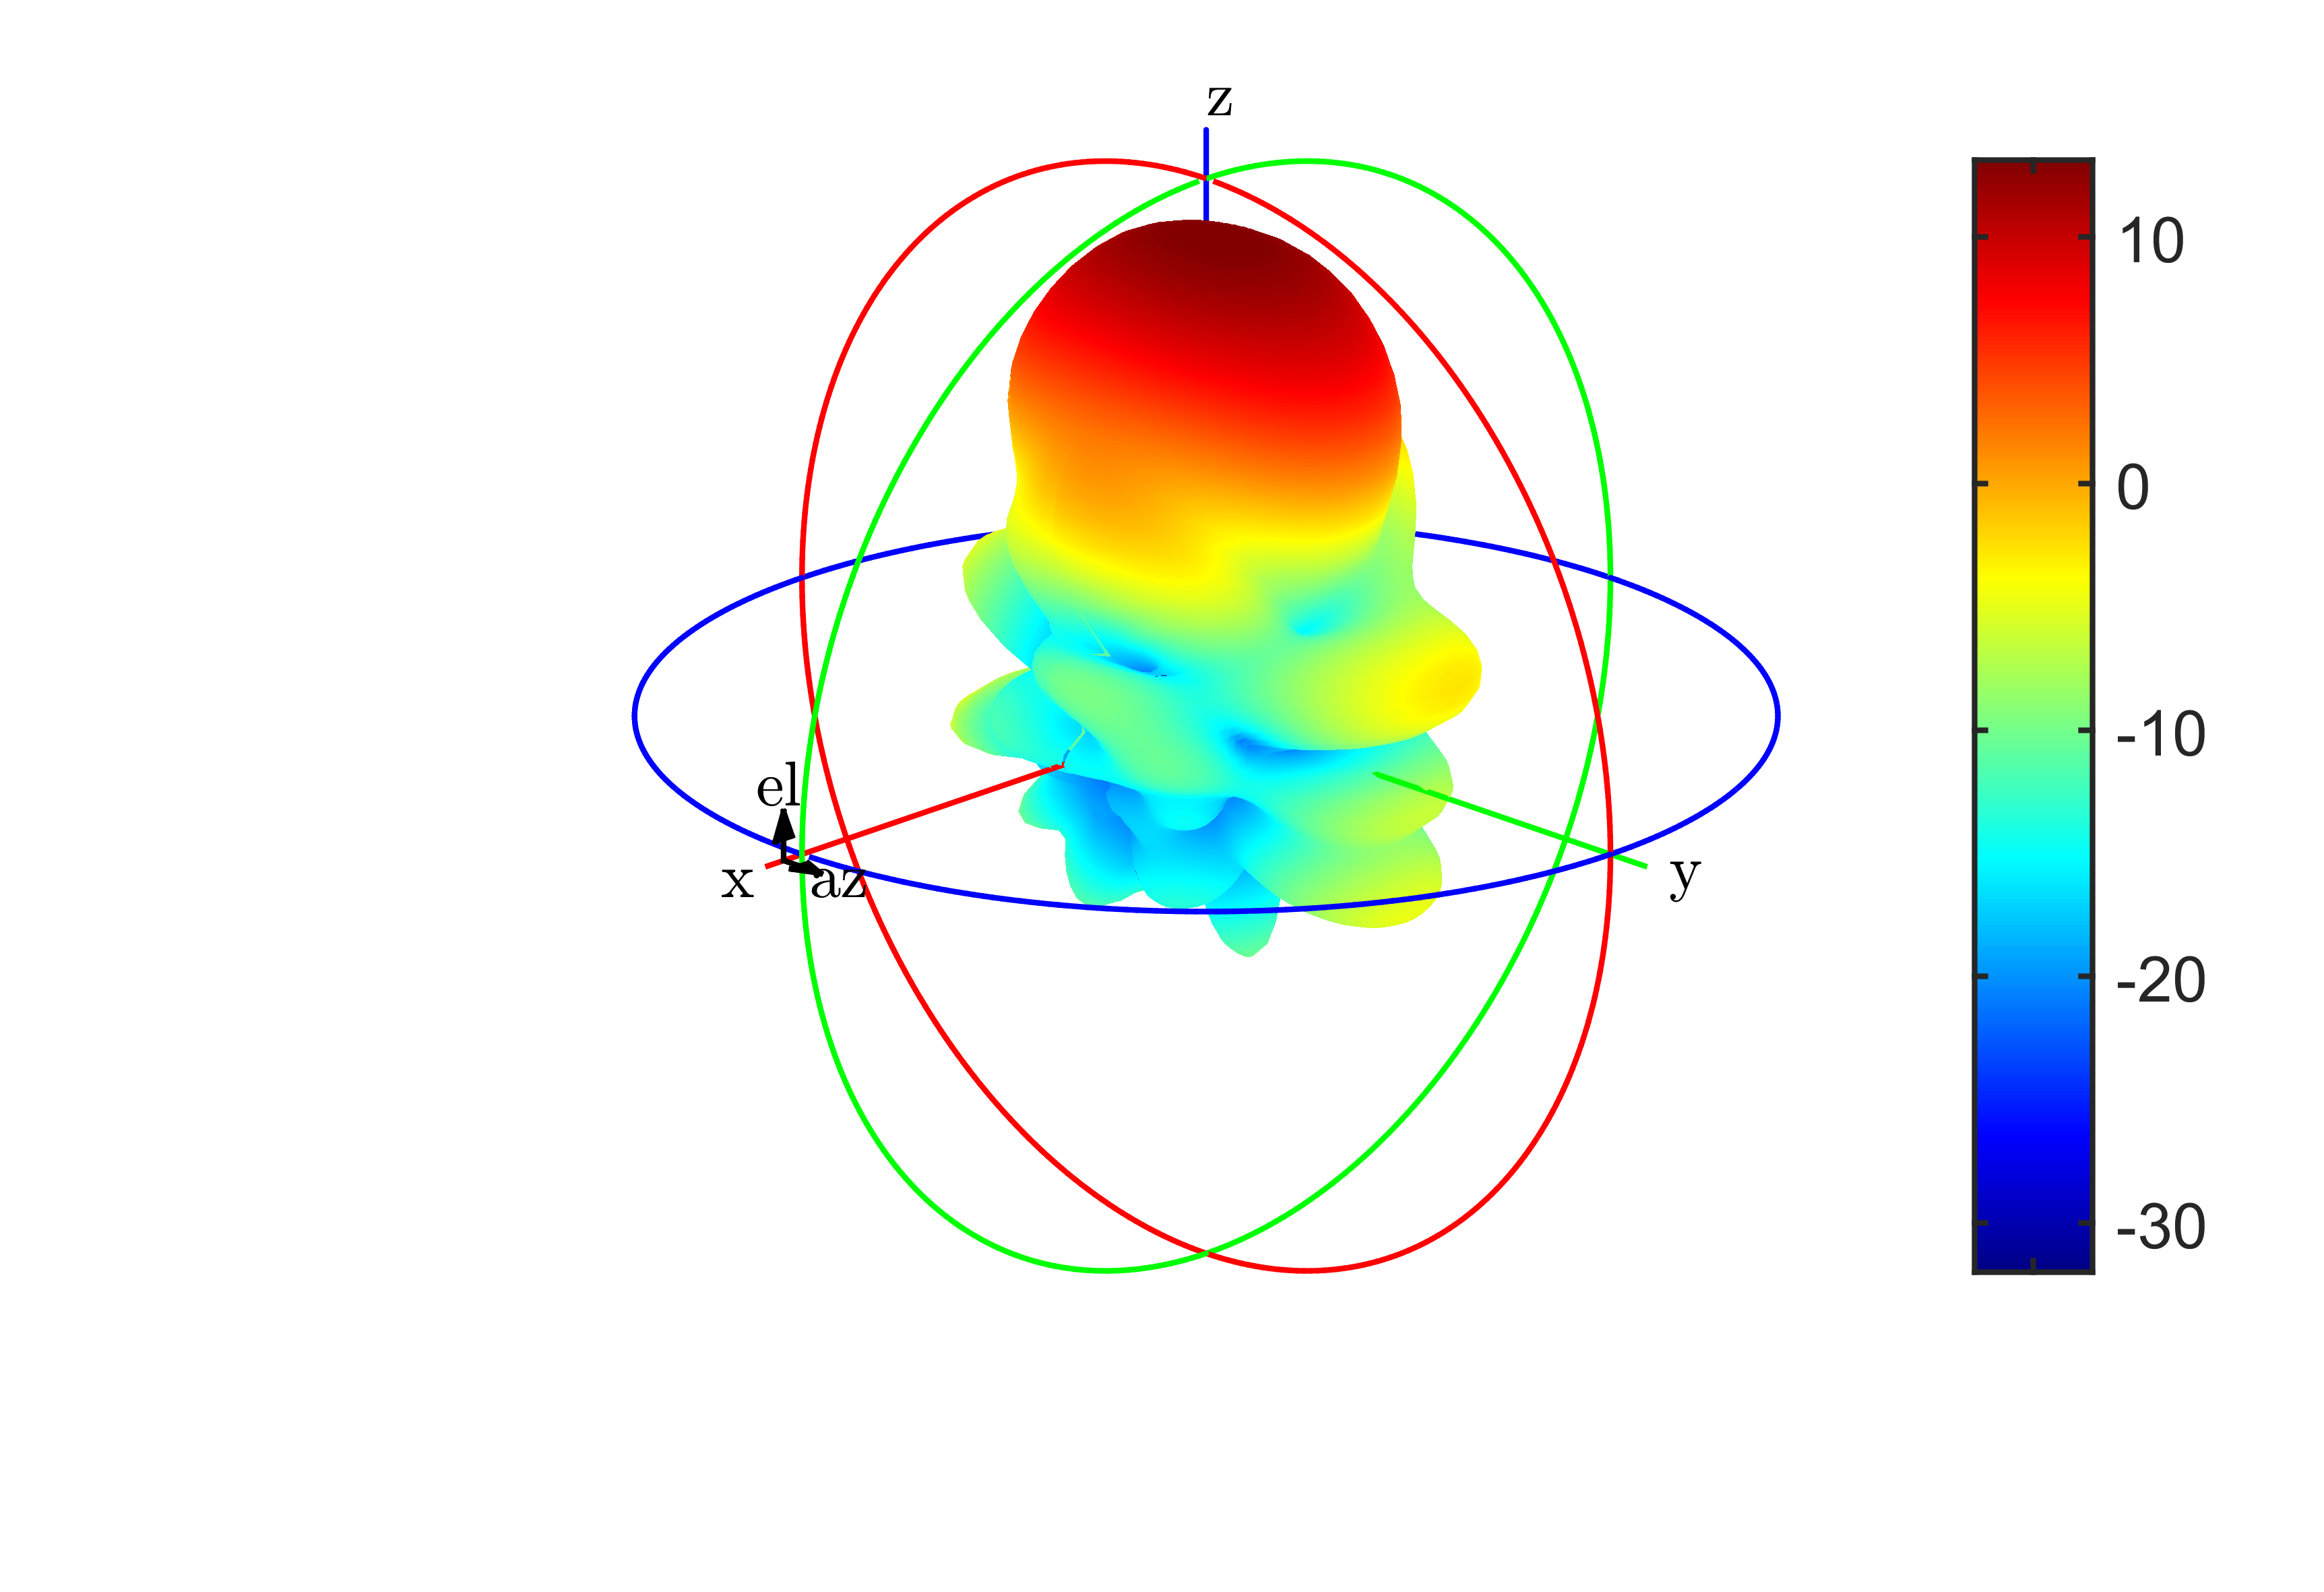
\includegraphics[scale = 0.5]{figures/measurement/antennas/array_4_0p4.png}
\caption{Farfield for $d = 0.4\lambda$. Maximum gain is 13.1dB}
    \label{fig:chamber_four_ant_ff:04}
  \end{minipage}
\end{figure}

\begin{figure}[H]
  \centering
  \begin{minipage}[b]{0.5\textwidth}
	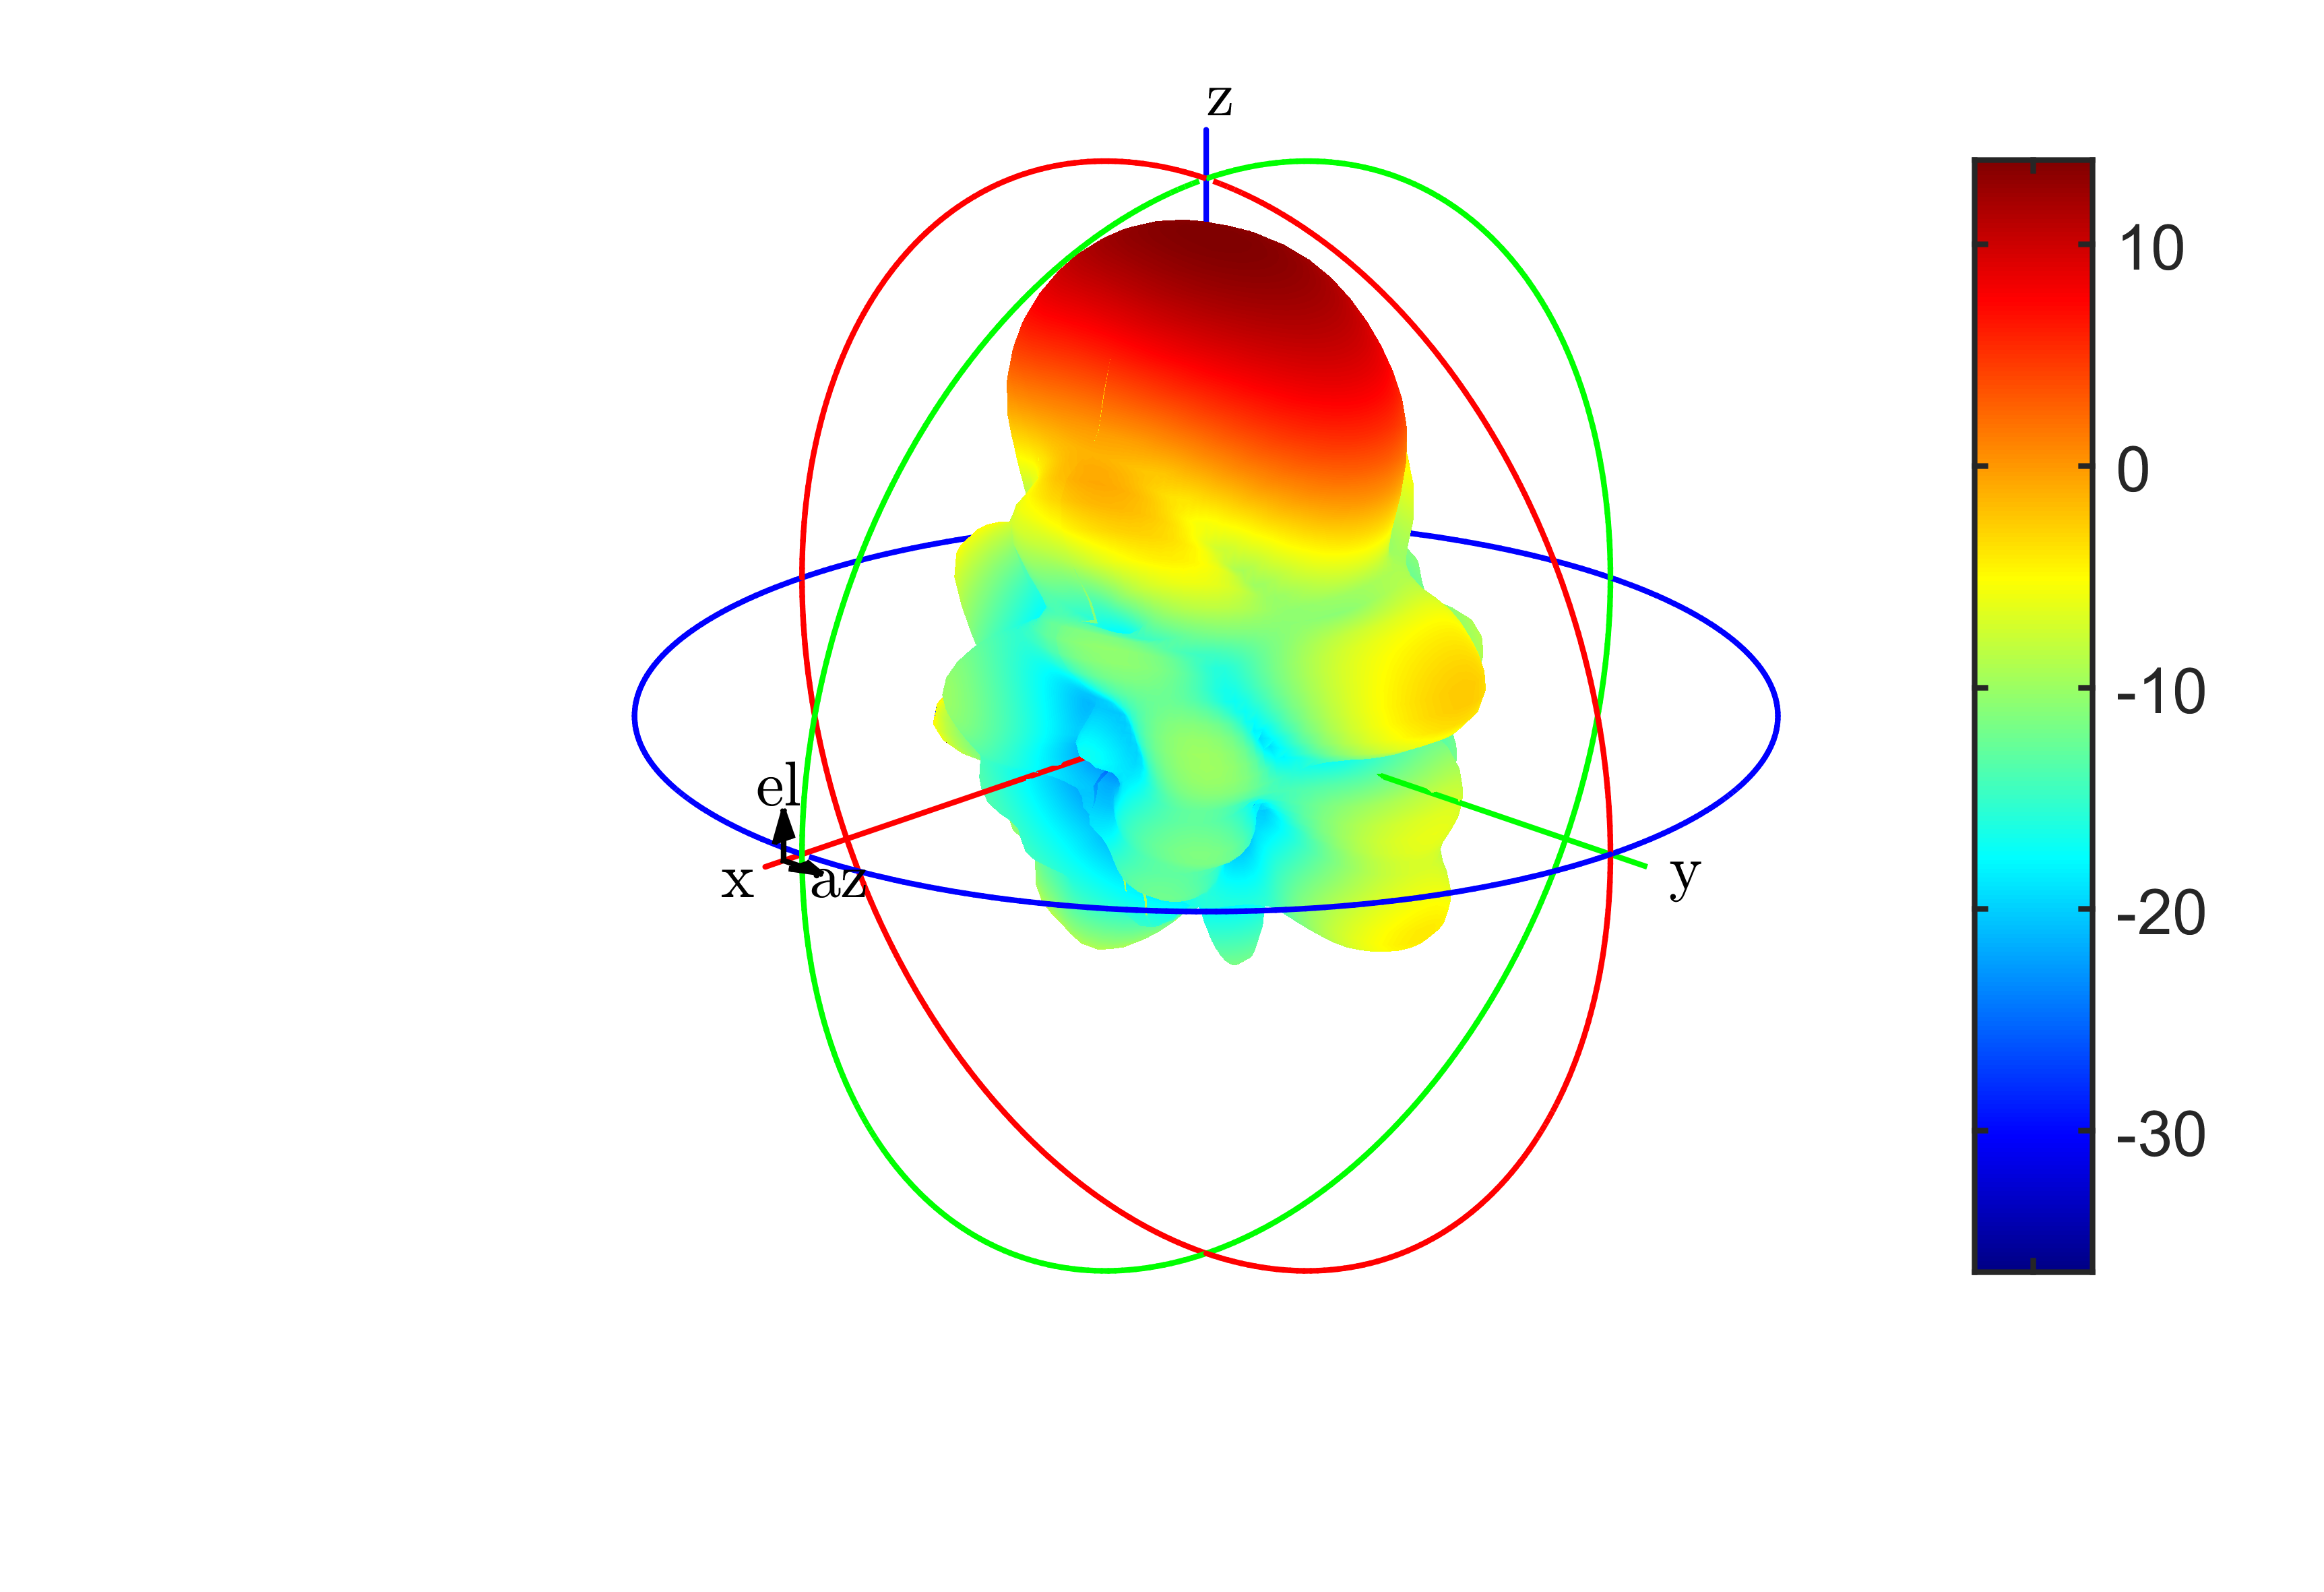
\includegraphics[scale = 0.5]{figures/measurement/antennas/array_4_0p5.png}
	\caption{Farfield for $d = 0.5\lambda$. Maximum gain is 13.8dB}
    \label{fig:chamber_four_ant_ff_05}
  \end{minipage}
  \hfill
  \begin{minipage}[b]{0.4\textwidth}
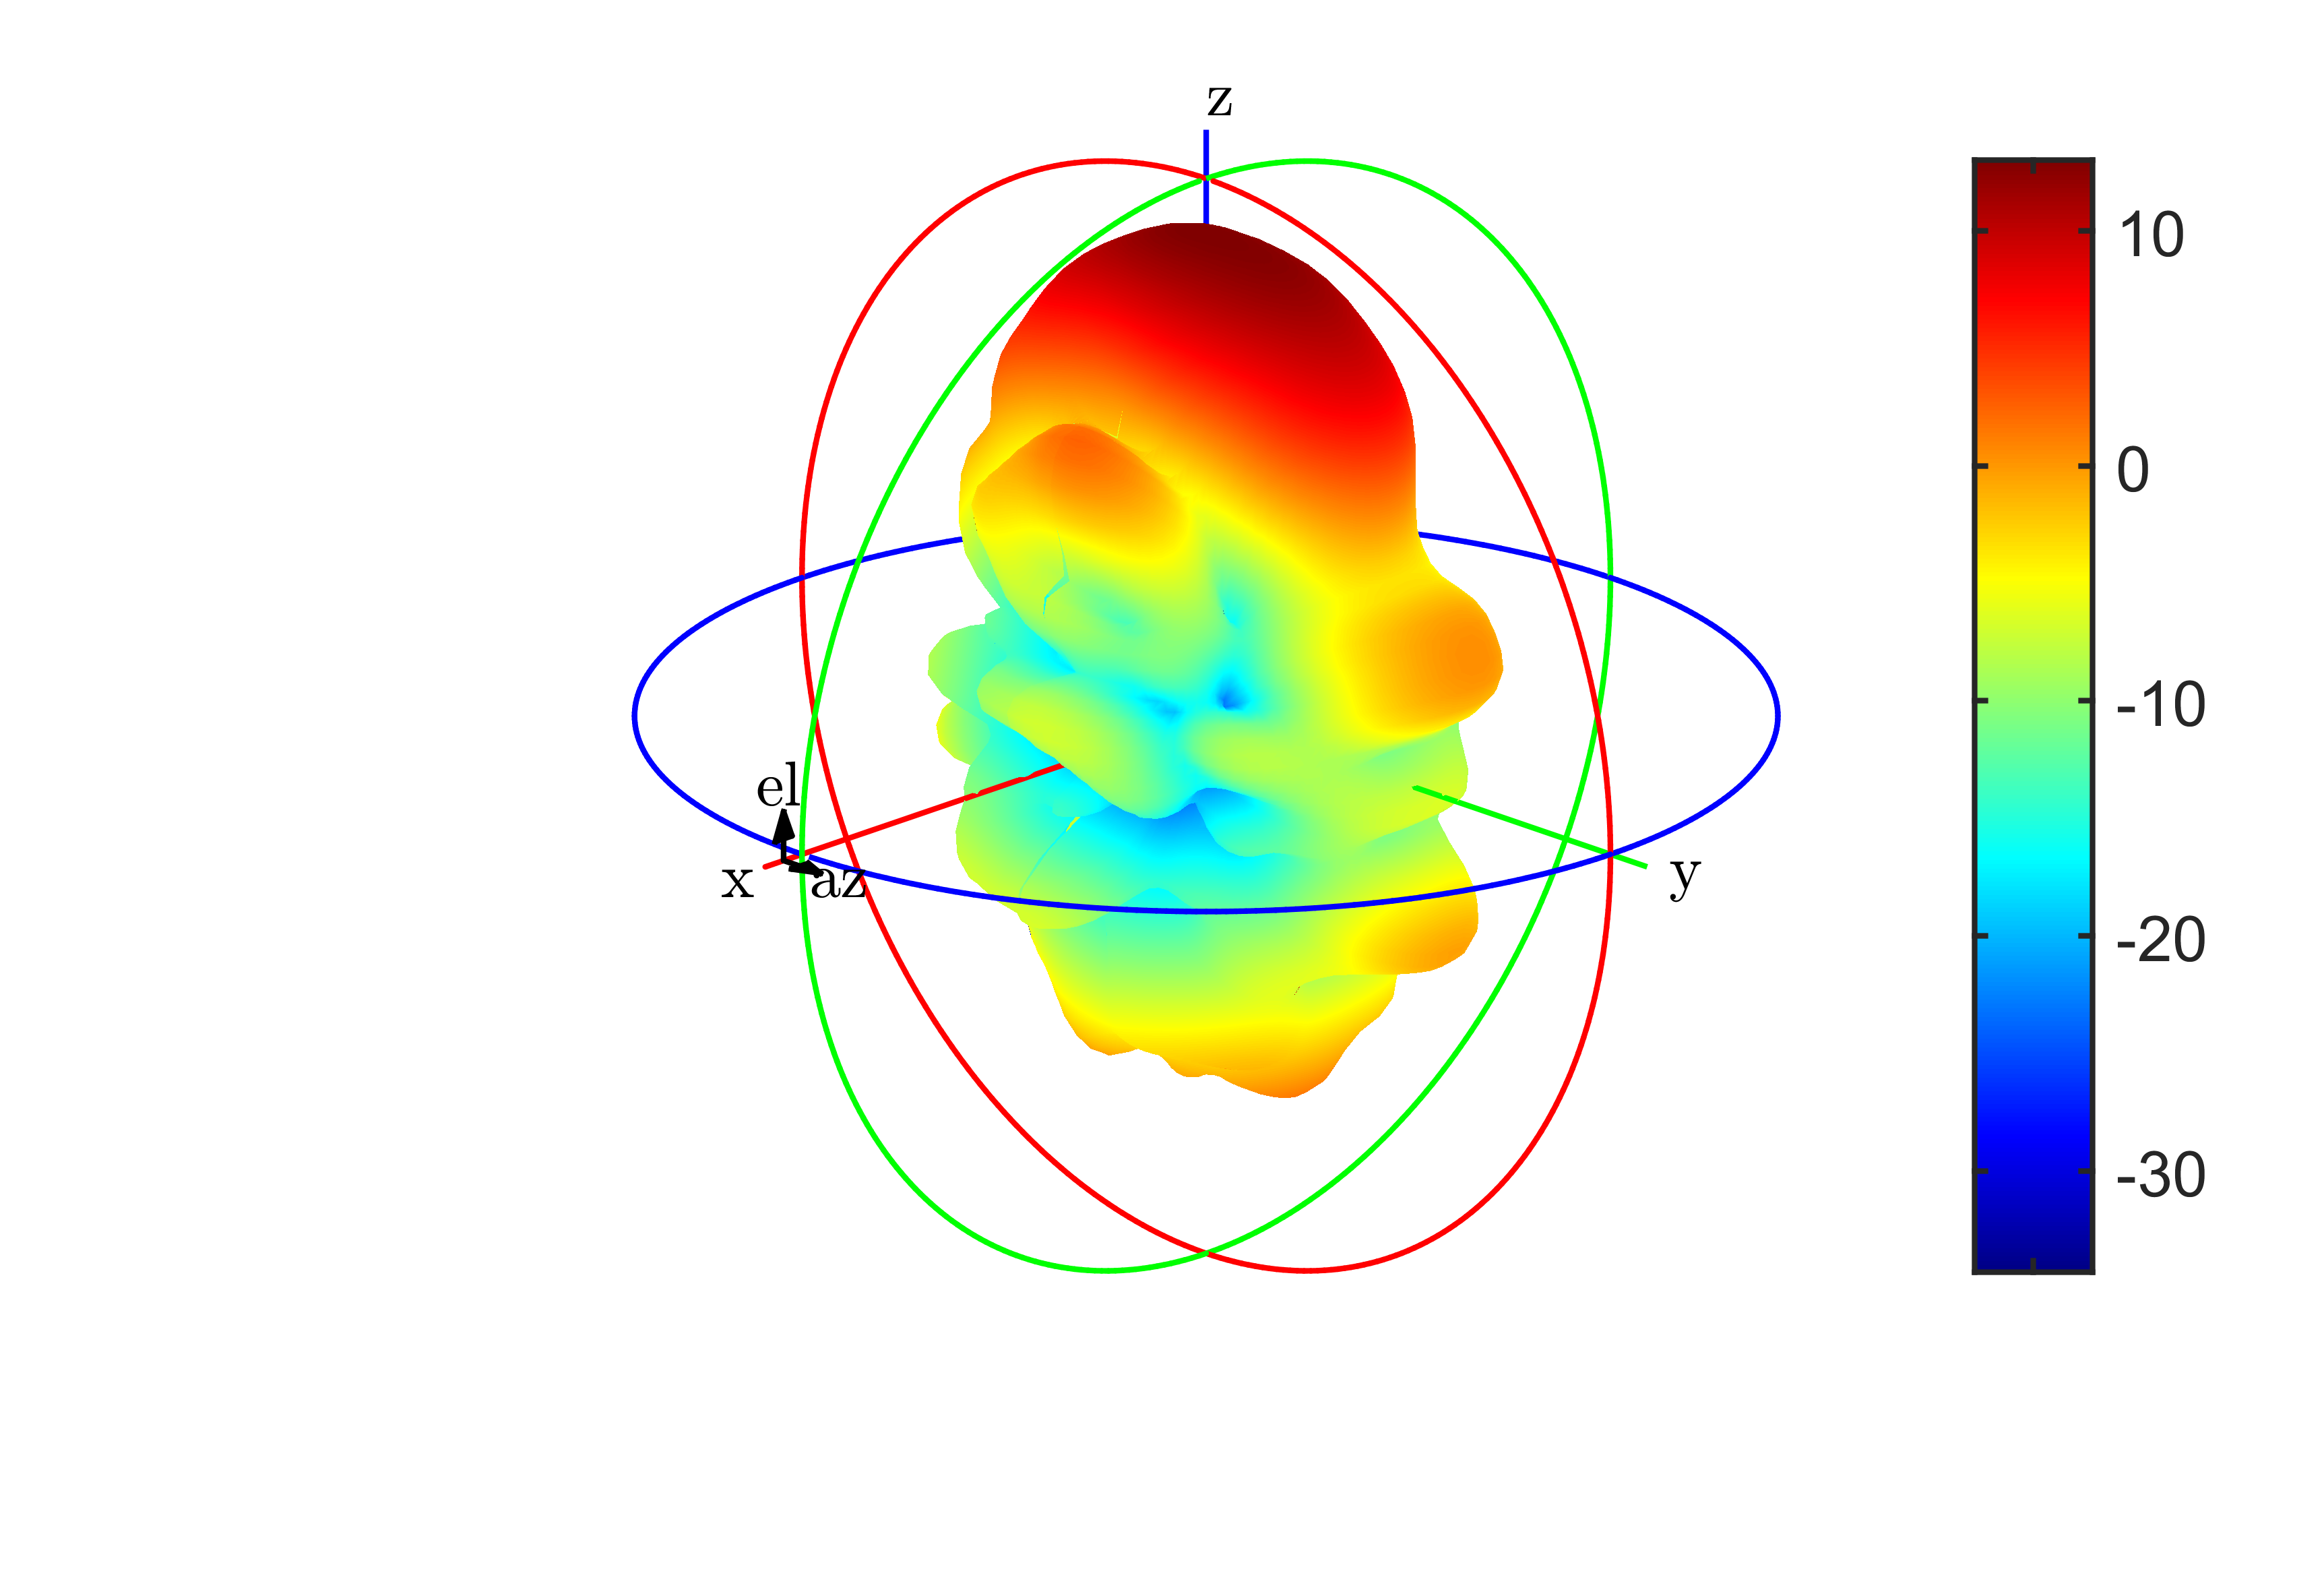
\includegraphics[scale = 0.5]{figures/measurement/antennas/array_4_0p6.png}
\caption{Farfield for $d = 0.6\lambda$. Maximum gain is 13.0dB}
    \label{fig:chamber_four_ant_ff:06}
  \end{minipage}
\end{figure}



\begin{figure}[H]
  \centering
  \begin{minipage}[b]{0.5\textwidth}
	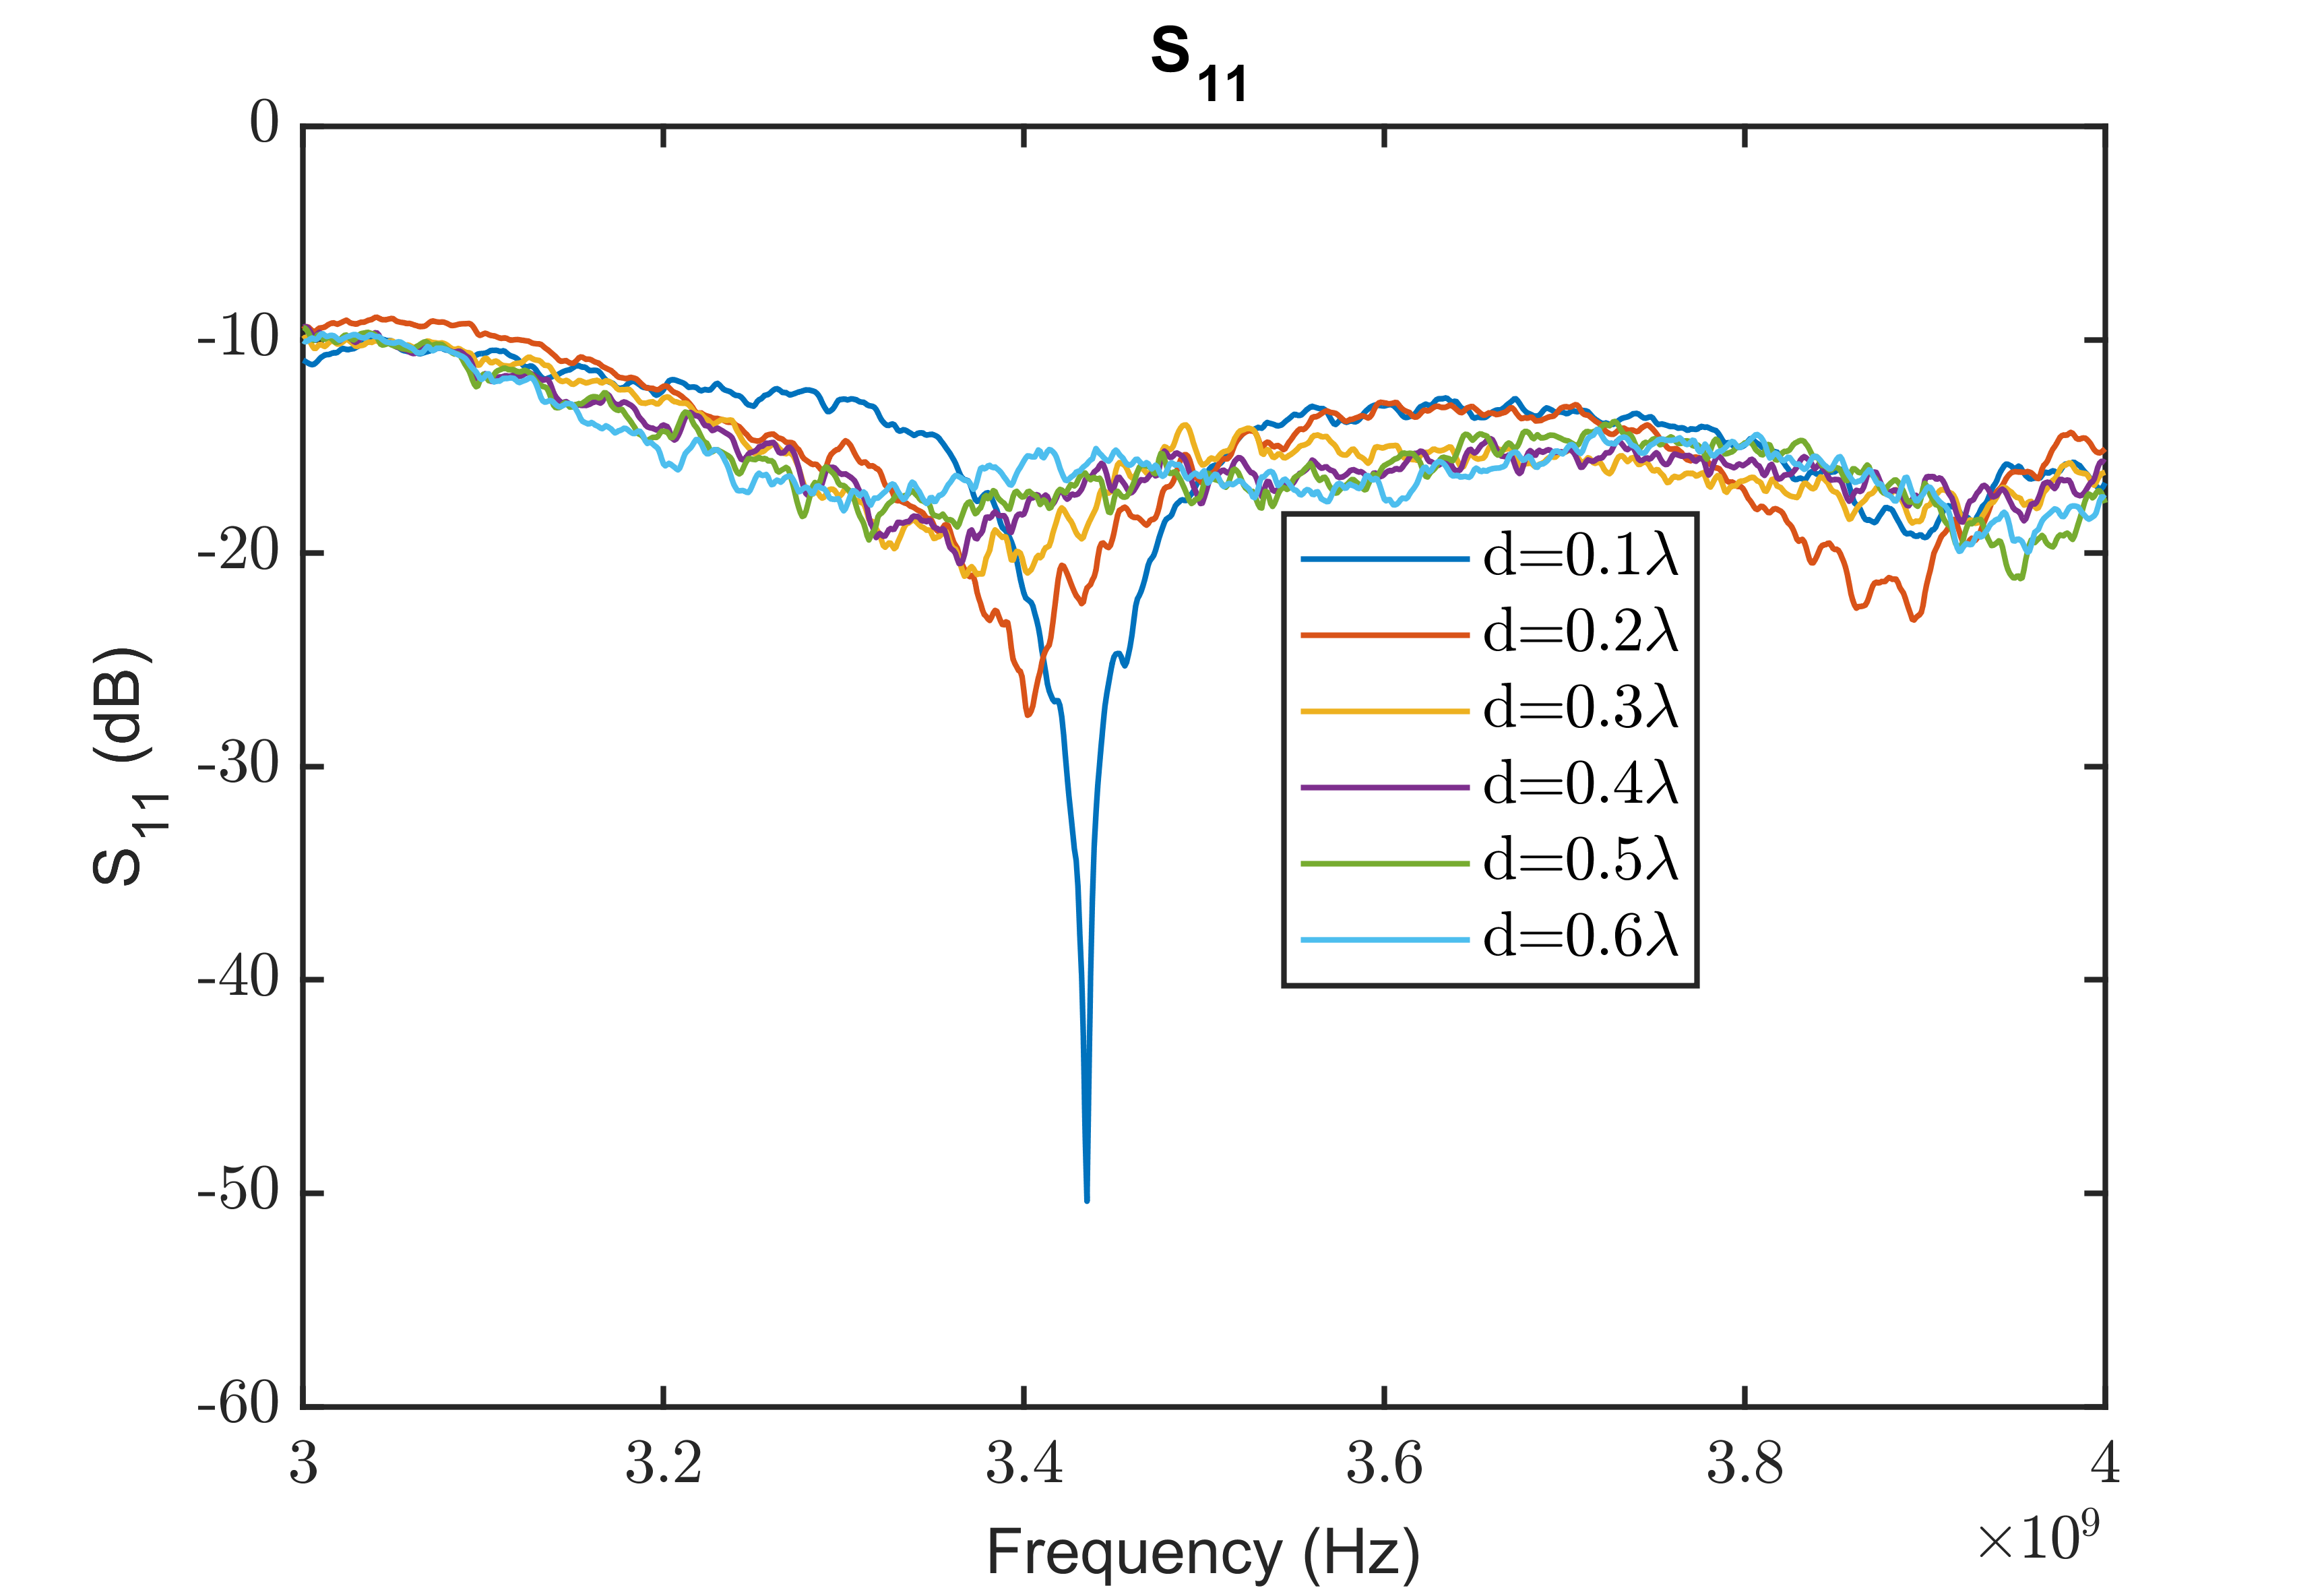
\includegraphics[scale = 0.5]{figures/measurement/antennas/spar_four_ant_s11.png}
	\caption{Measured $S_{11}$ with four antennas}
    \label{fig:chamber_four_ant_s11}
  \end{minipage}
  \hfill
  \begin{minipage}[b]{0.4\textwidth}
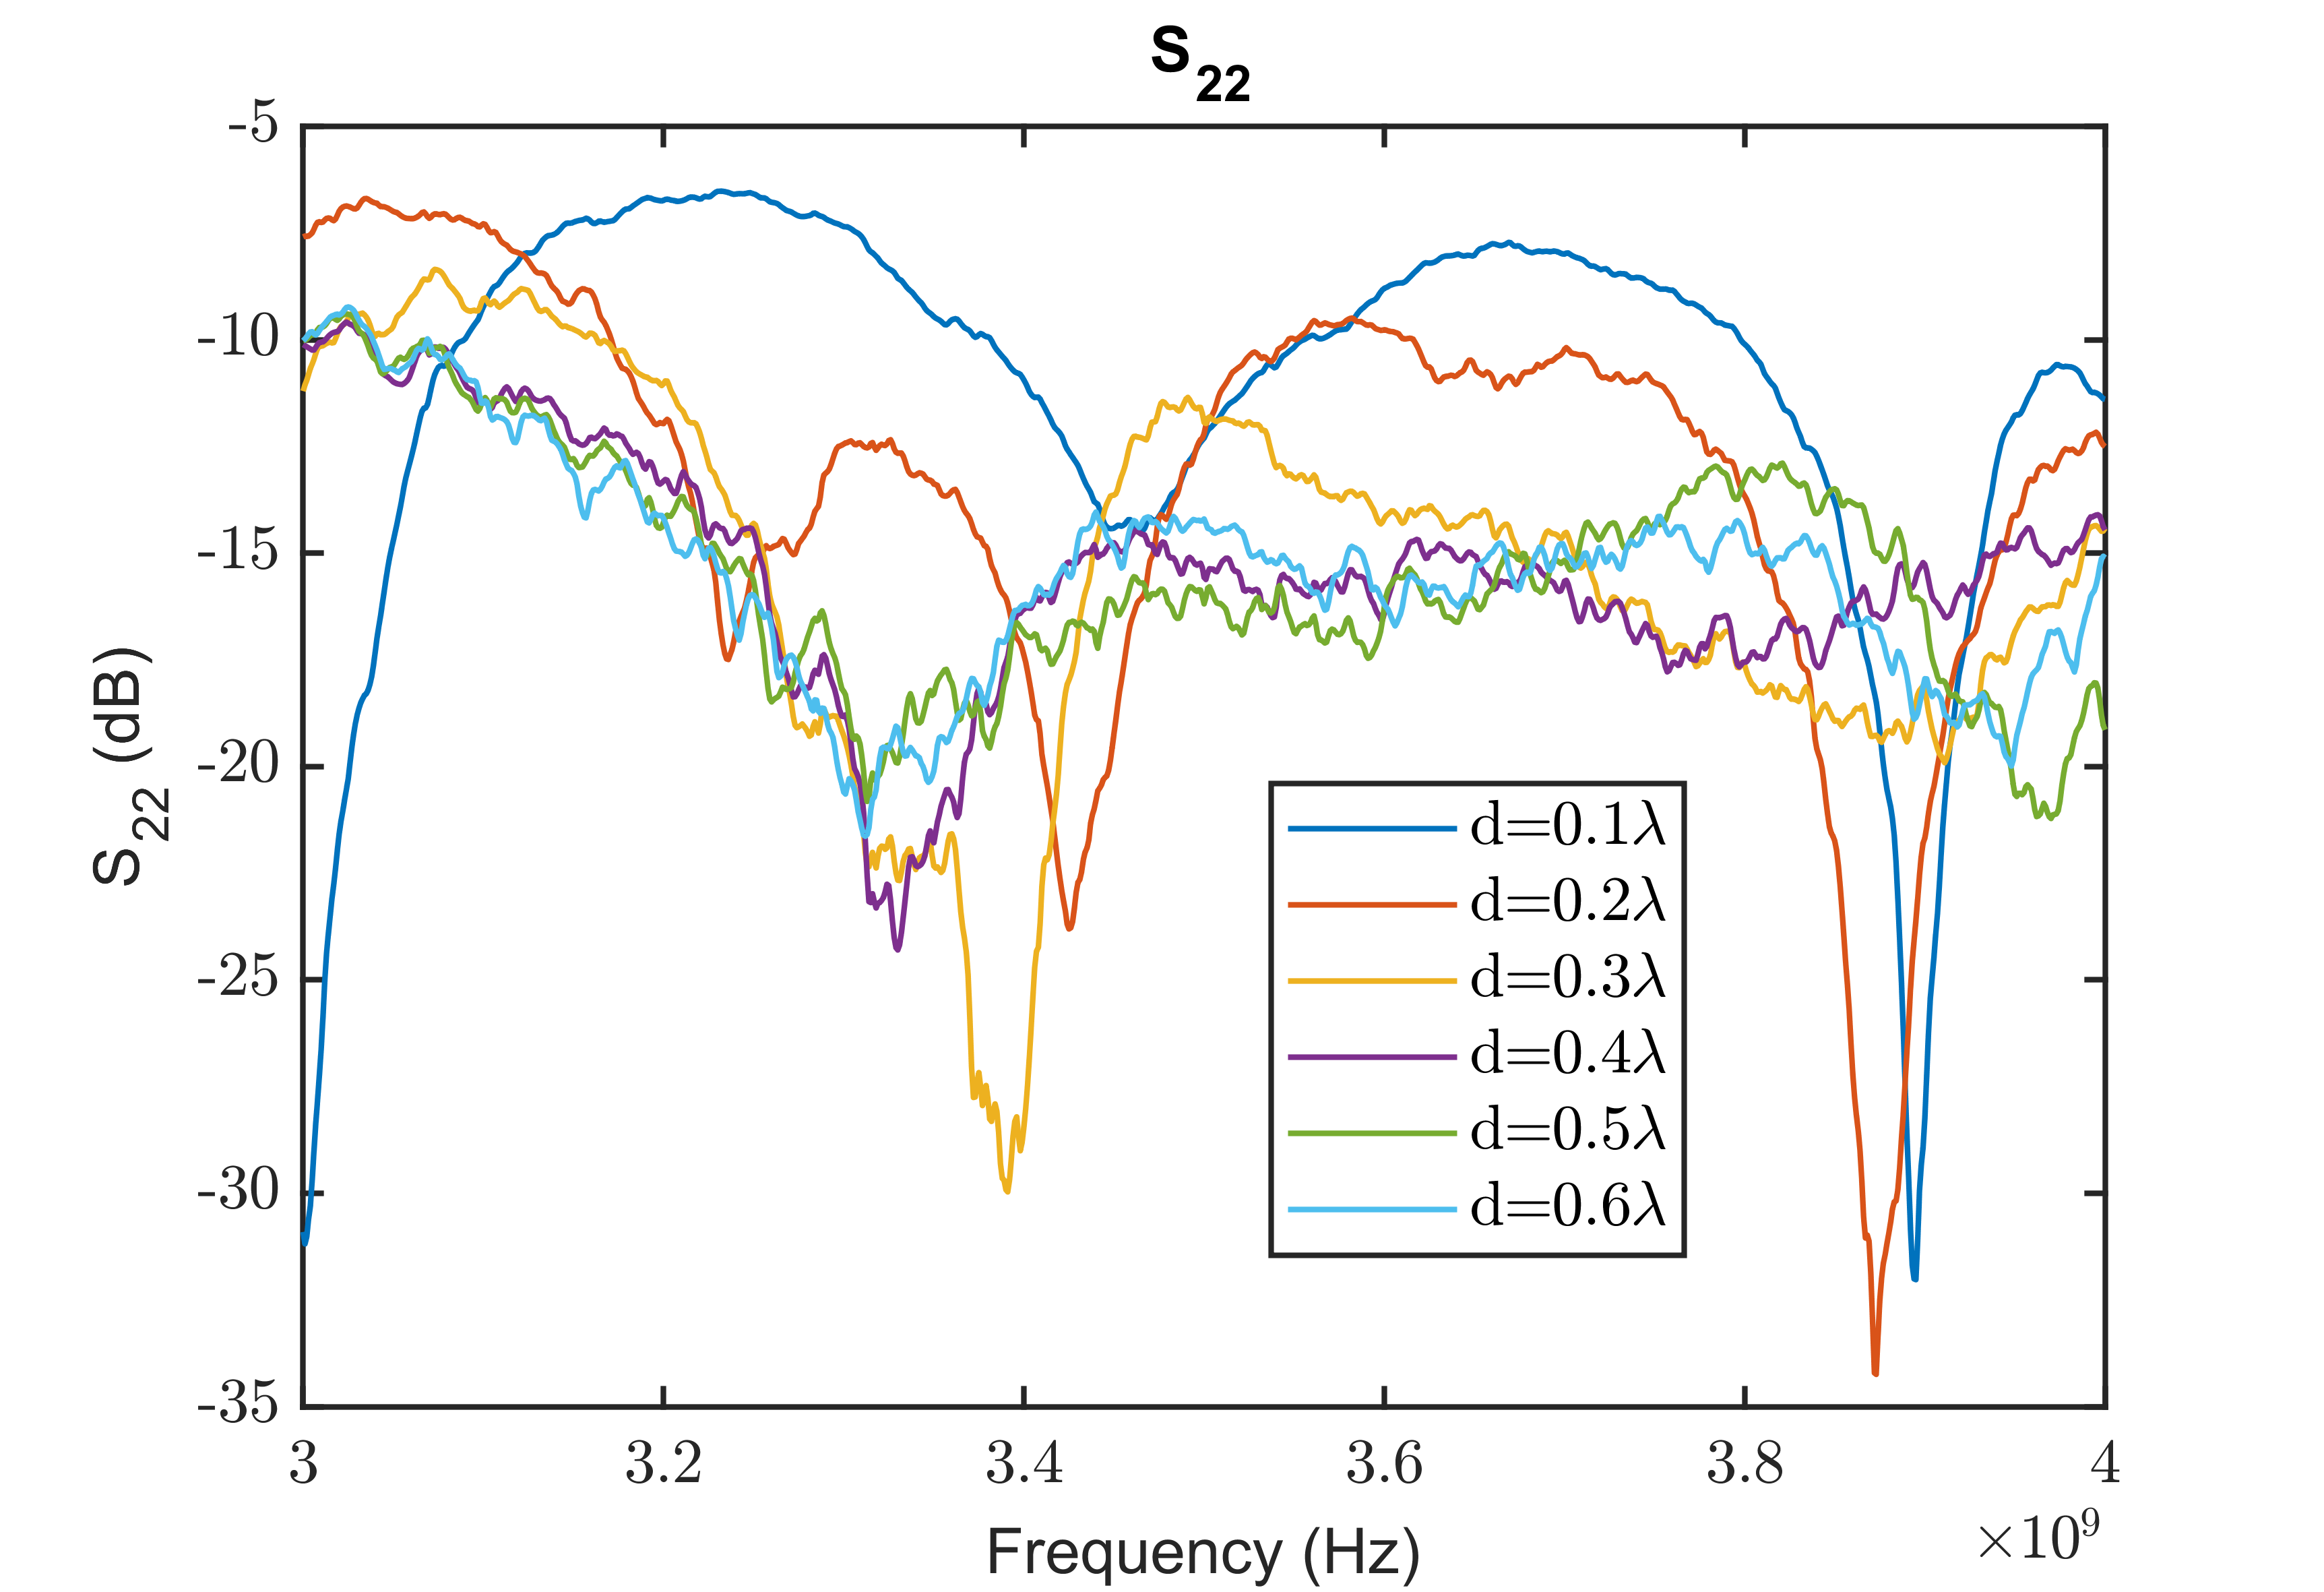
\includegraphics[scale = 0.5]{figures/measurement/antennas/spar_four_ant_s22.png}
\caption{Measured $S_{22}$ with four antennas}
    \label{fig:chamber_four_ant_s22}
  \end{minipage}
\end{figure}


\begin{figure}[H]
  \centering
  \begin{minipage}[b]{0.5\textwidth}
	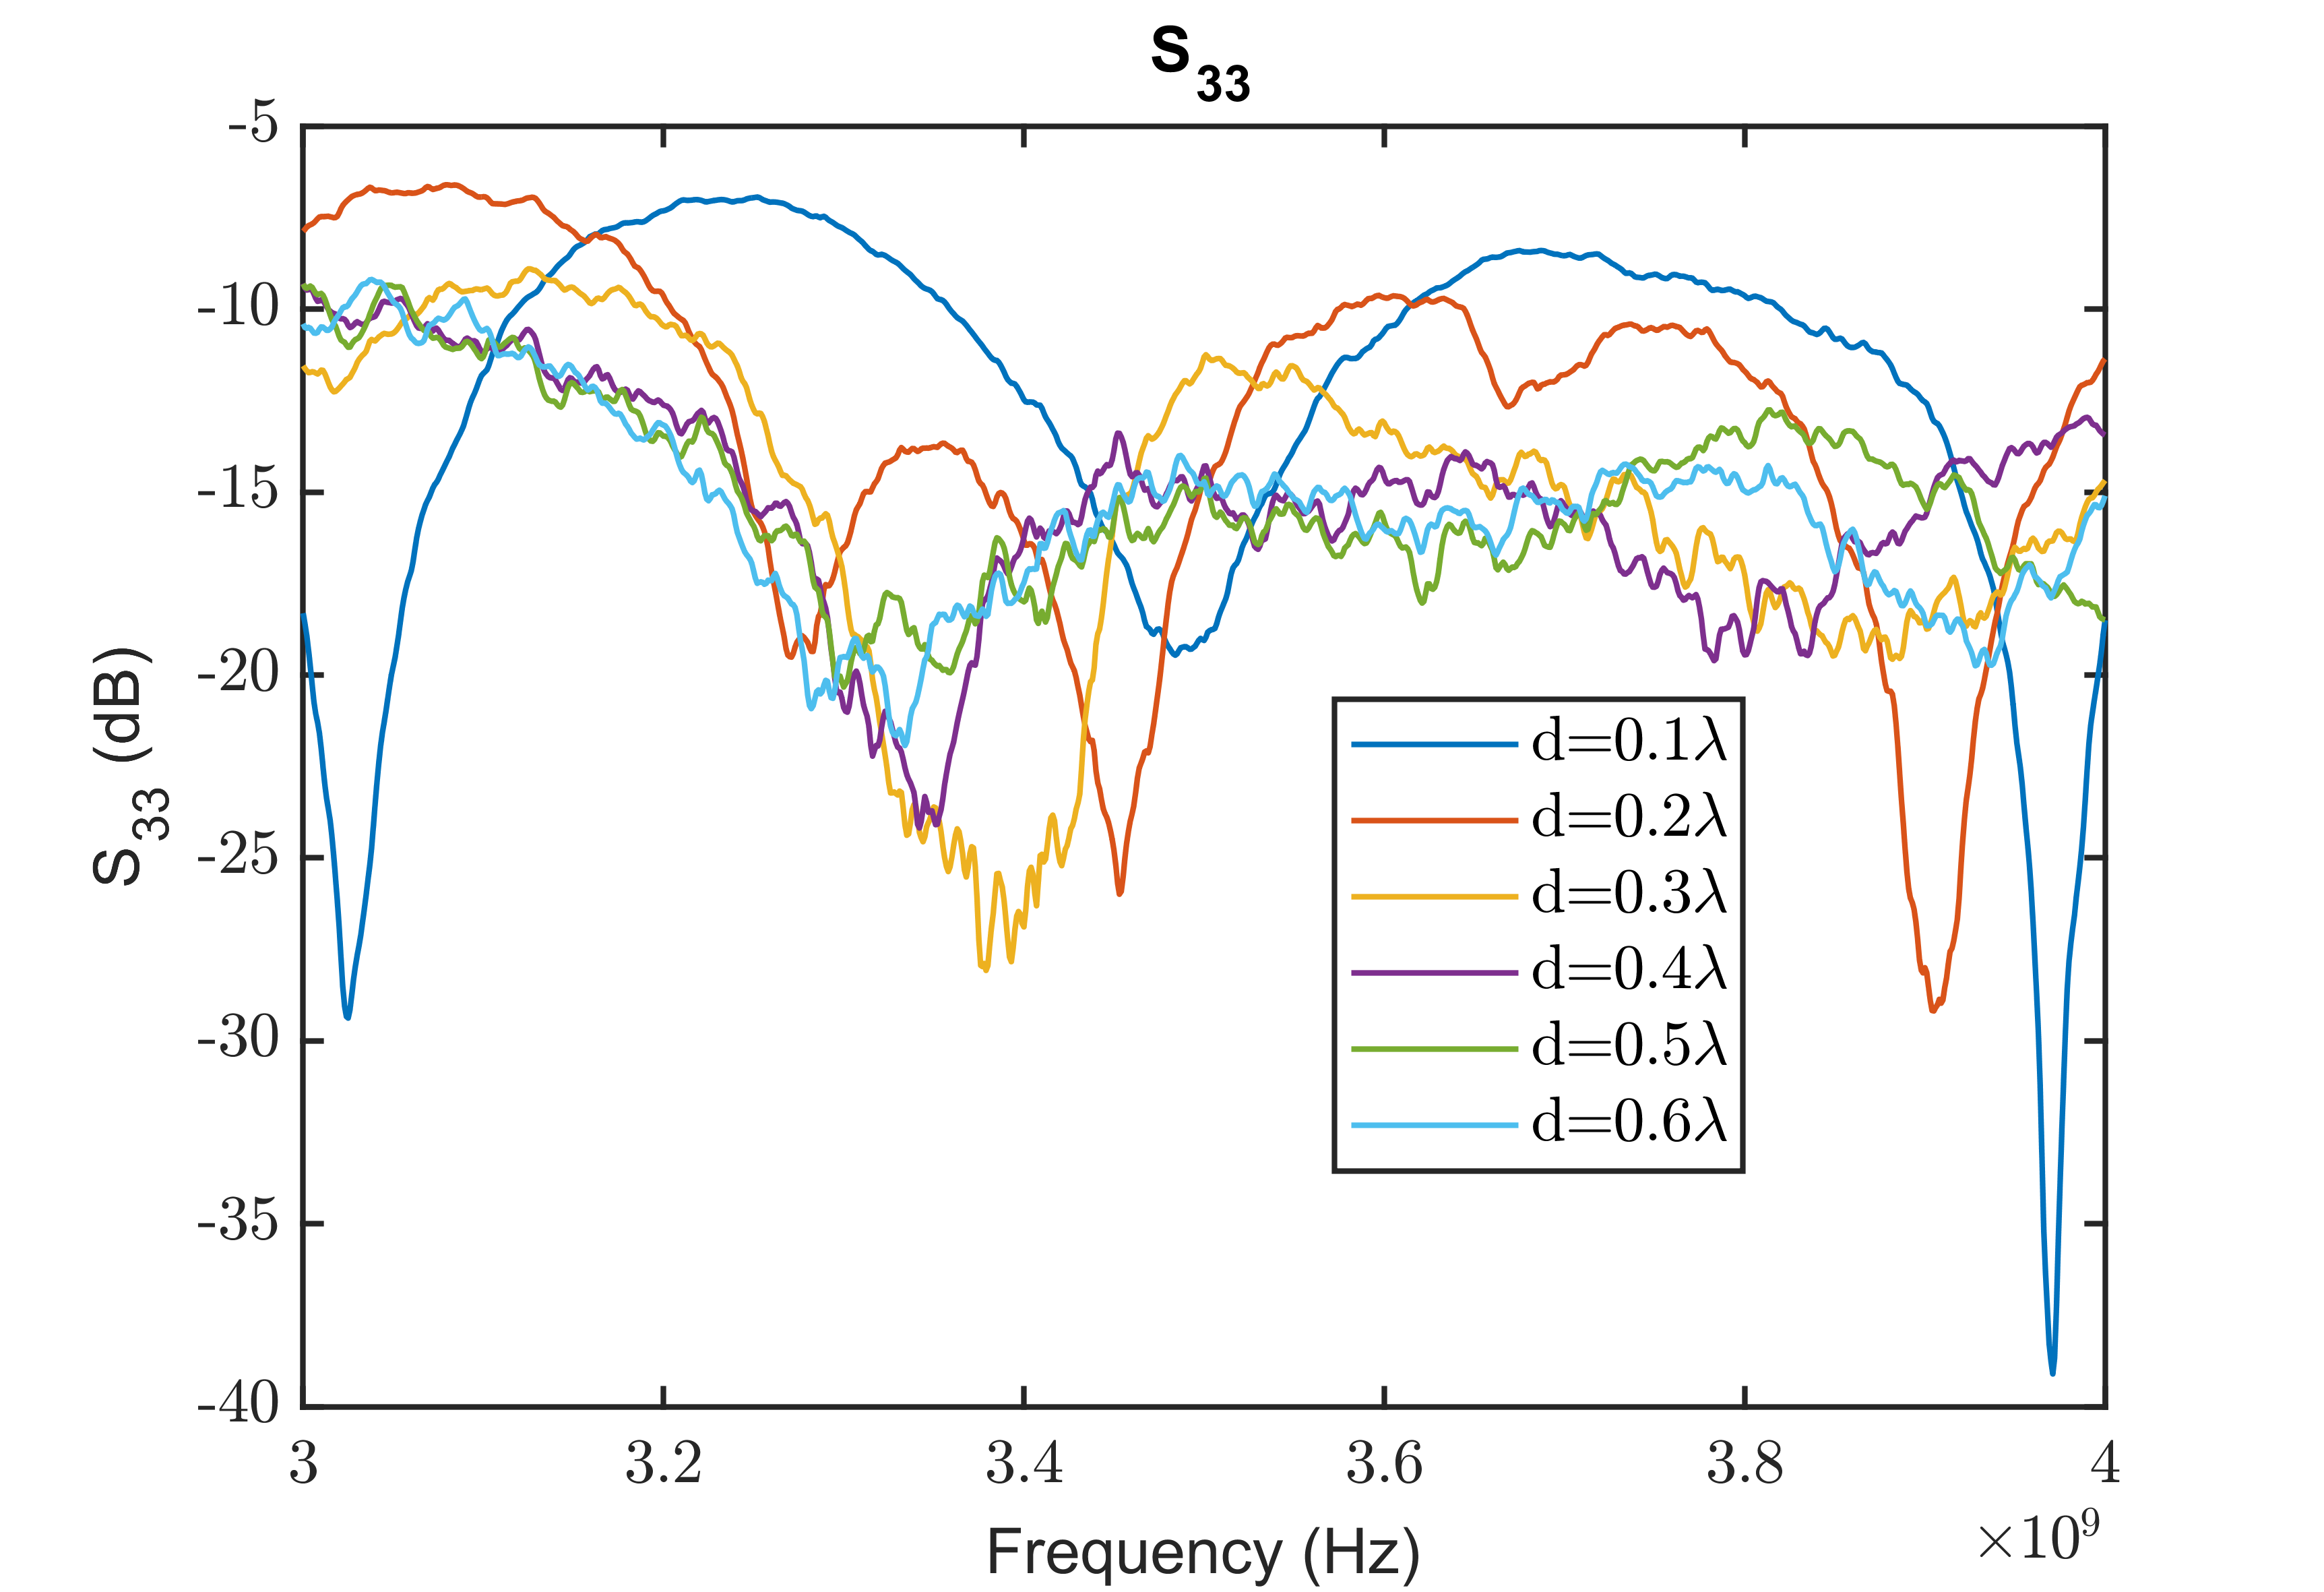
\includegraphics[scale = 0.5]{figures/measurement/antennas/spar_four_ant_s33.png}
	\caption{Measured $S_{33}$ with four antennas}
    \label{fig:chamber_four_ant_s33}
  \end{minipage}
  \hfill
  \begin{minipage}[b]{0.4\textwidth}
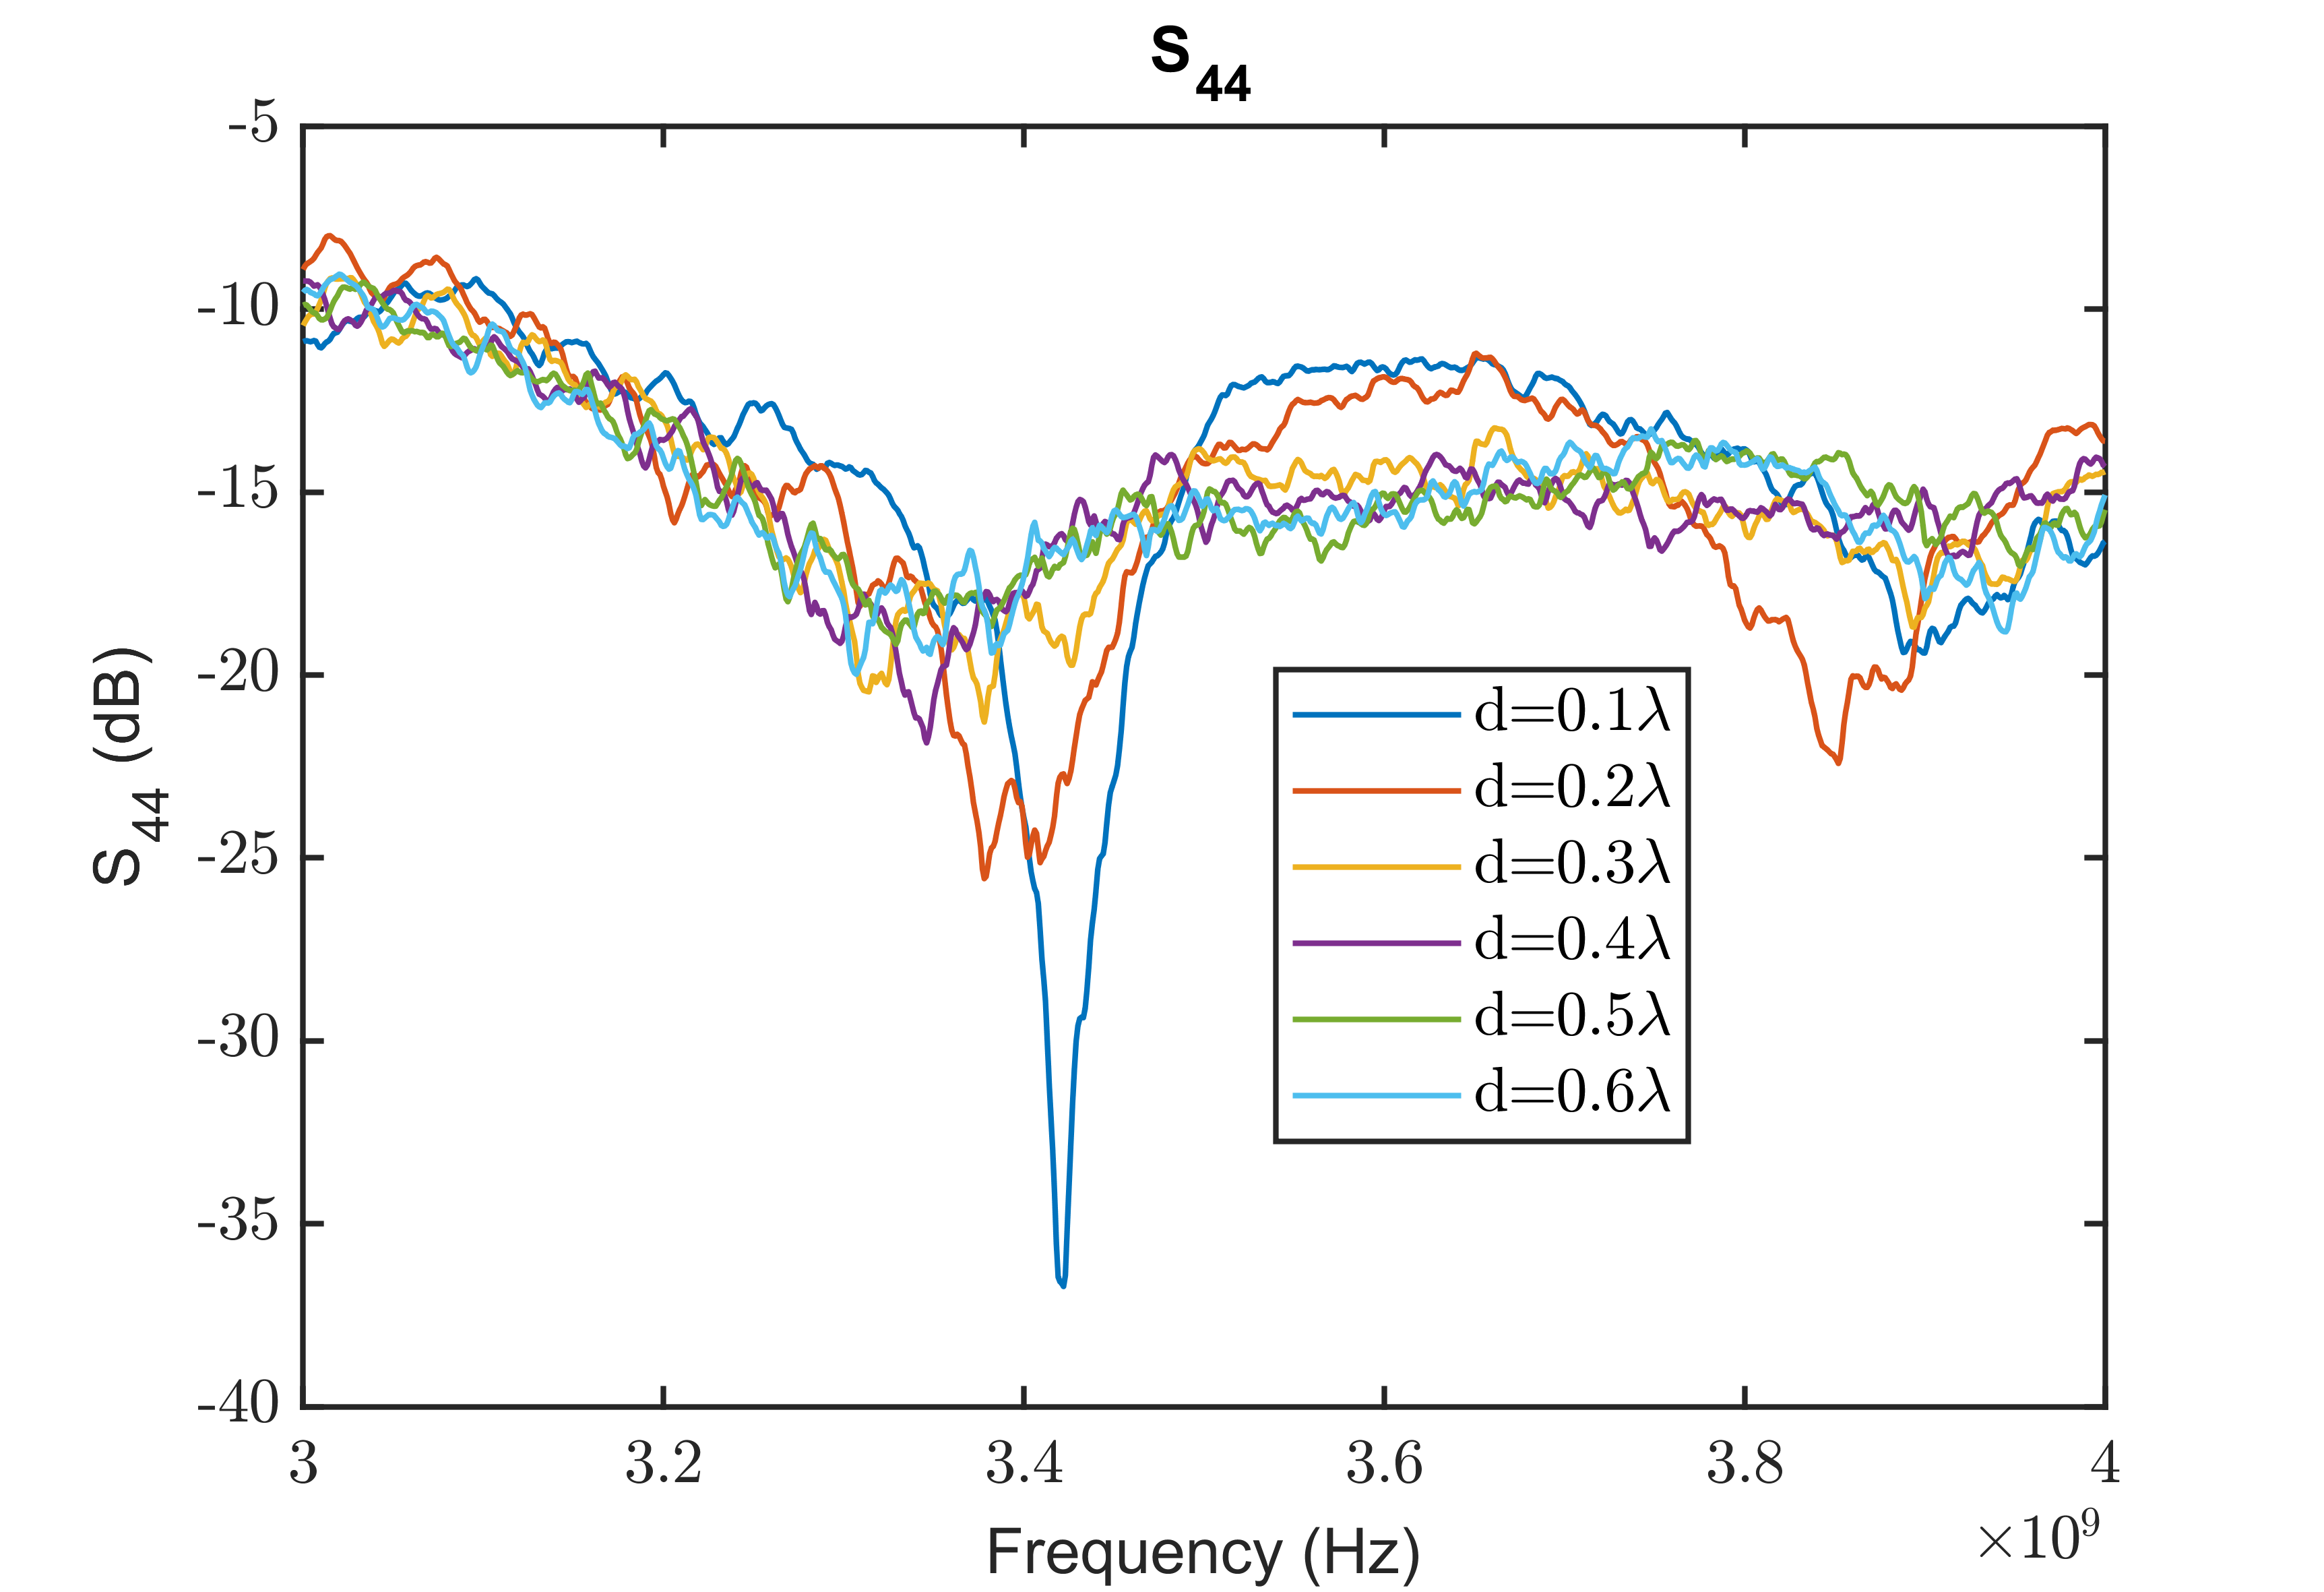
\includegraphics[scale = 0.5]{figures/measurement/antennas/spar_four_ant_s44.png}
\caption{Measured $S_{44}$ with four antennas}
    \label{fig:chamber_four_ant_s44}
  \end{minipage}
\end{figure}


\begin{figure}[H]
  \centering
  \begin{minipage}[b]{0.5\textwidth}
	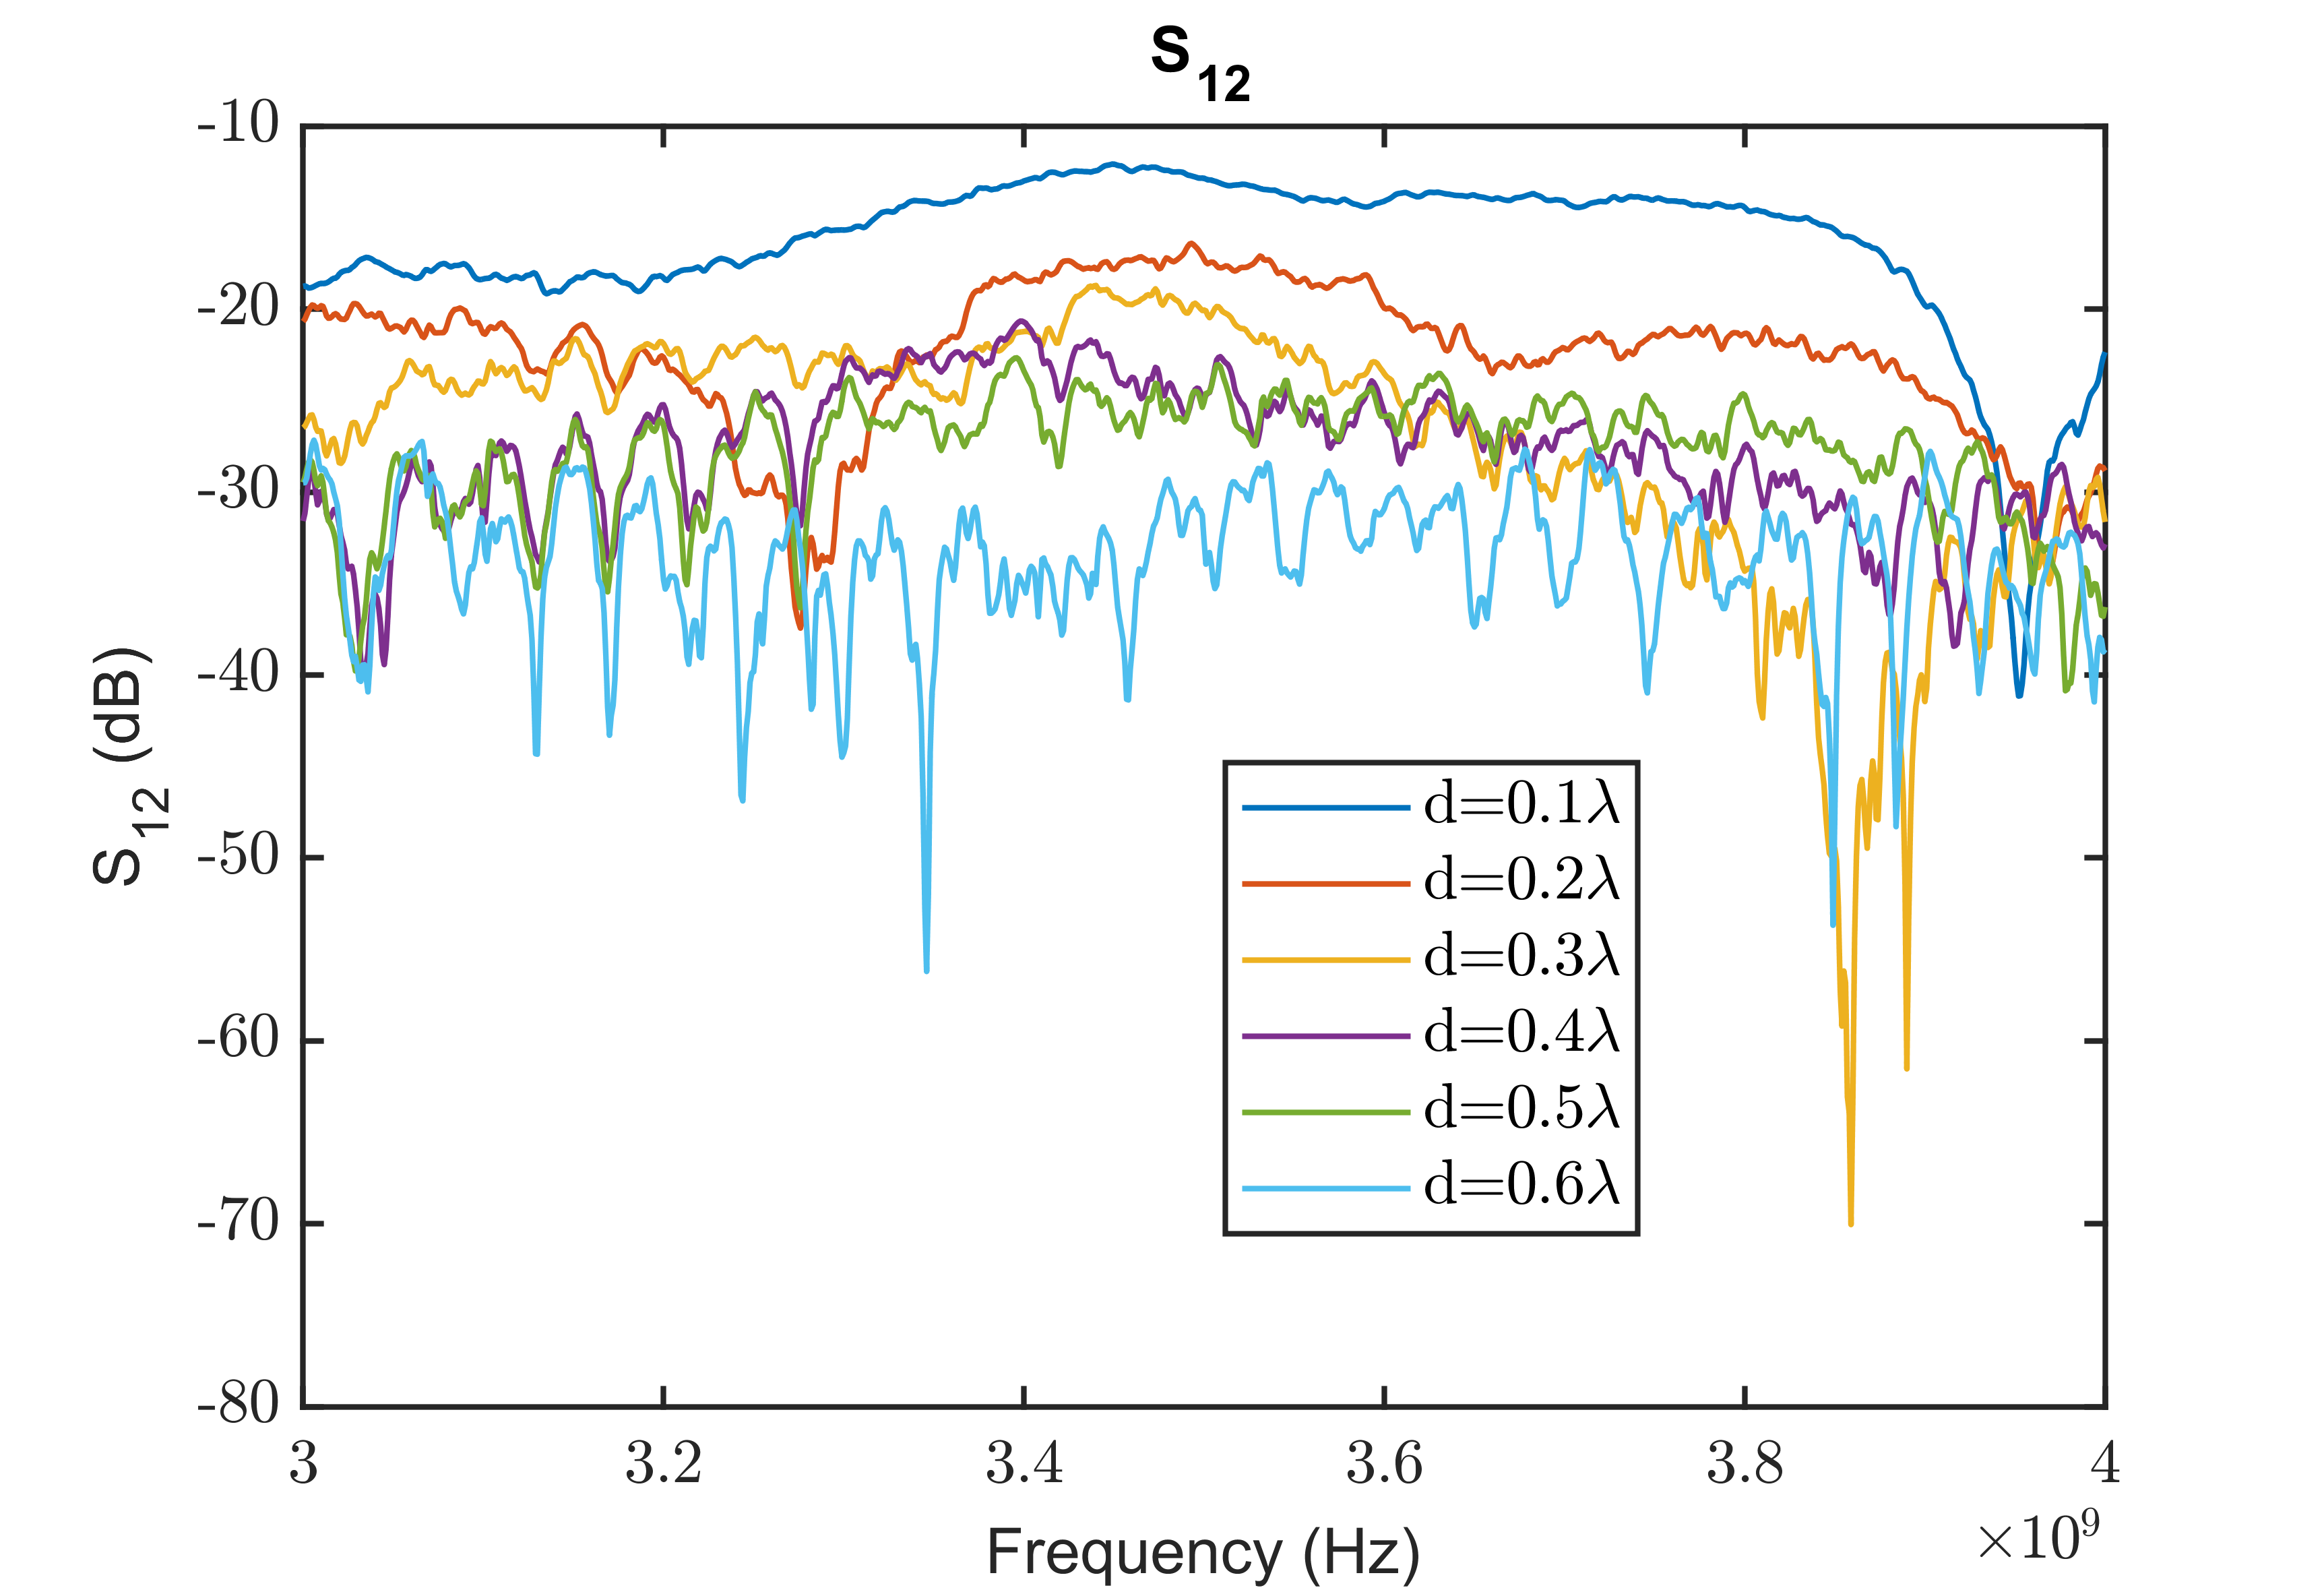
\includegraphics[scale = 0.5]{figures/measurement/antennas/spar_four_ant_s12.png}
	\caption{Measured $S_{12}$ with four antennas}
    \label{fig:chamber_four_ant_s12}
  \end{minipage}
  \hfill
  \begin{minipage}[b]{0.4\textwidth}
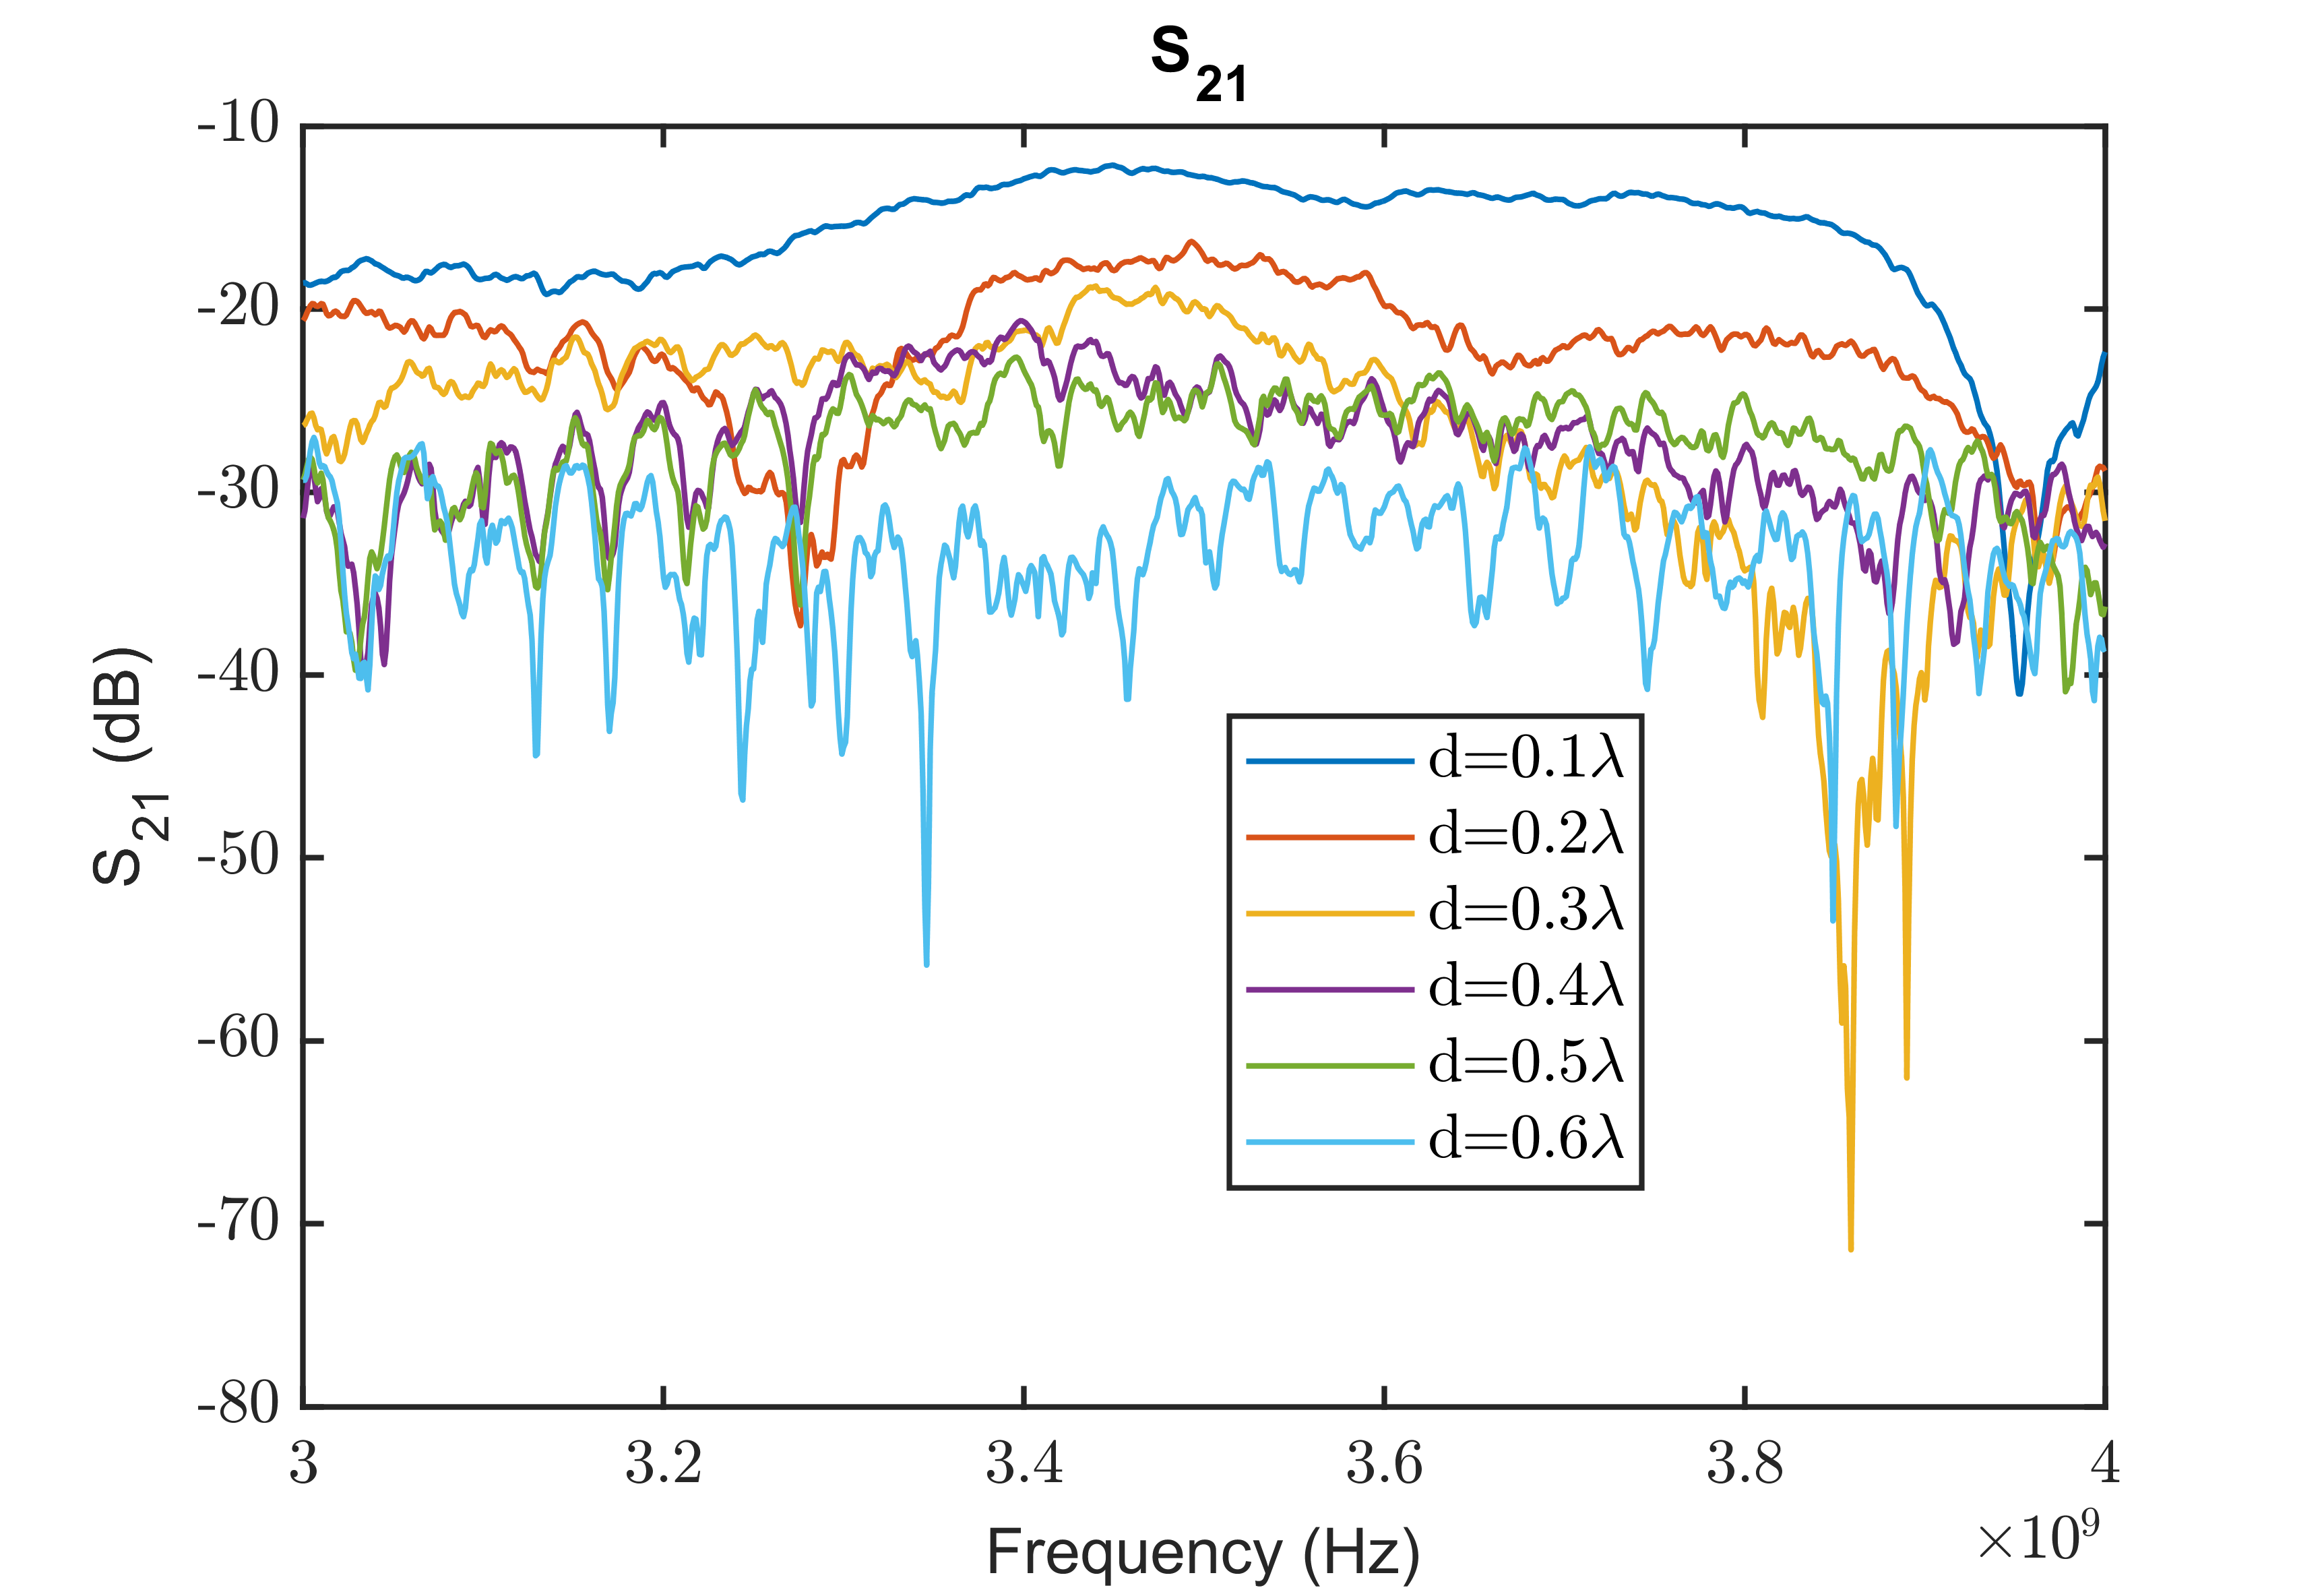
\includegraphics[scale = 0.5]{figures/measurement/antennas/spar_four_ant_s21.png}
\caption{Measured $S_{21}$ with four antennas}
    \label{fig:chamber_four_ant_s21}
  \end{minipage}
\end{figure}

\begin{figure}[H]
  \centering
  \begin{minipage}[b]{0.5\textwidth}
	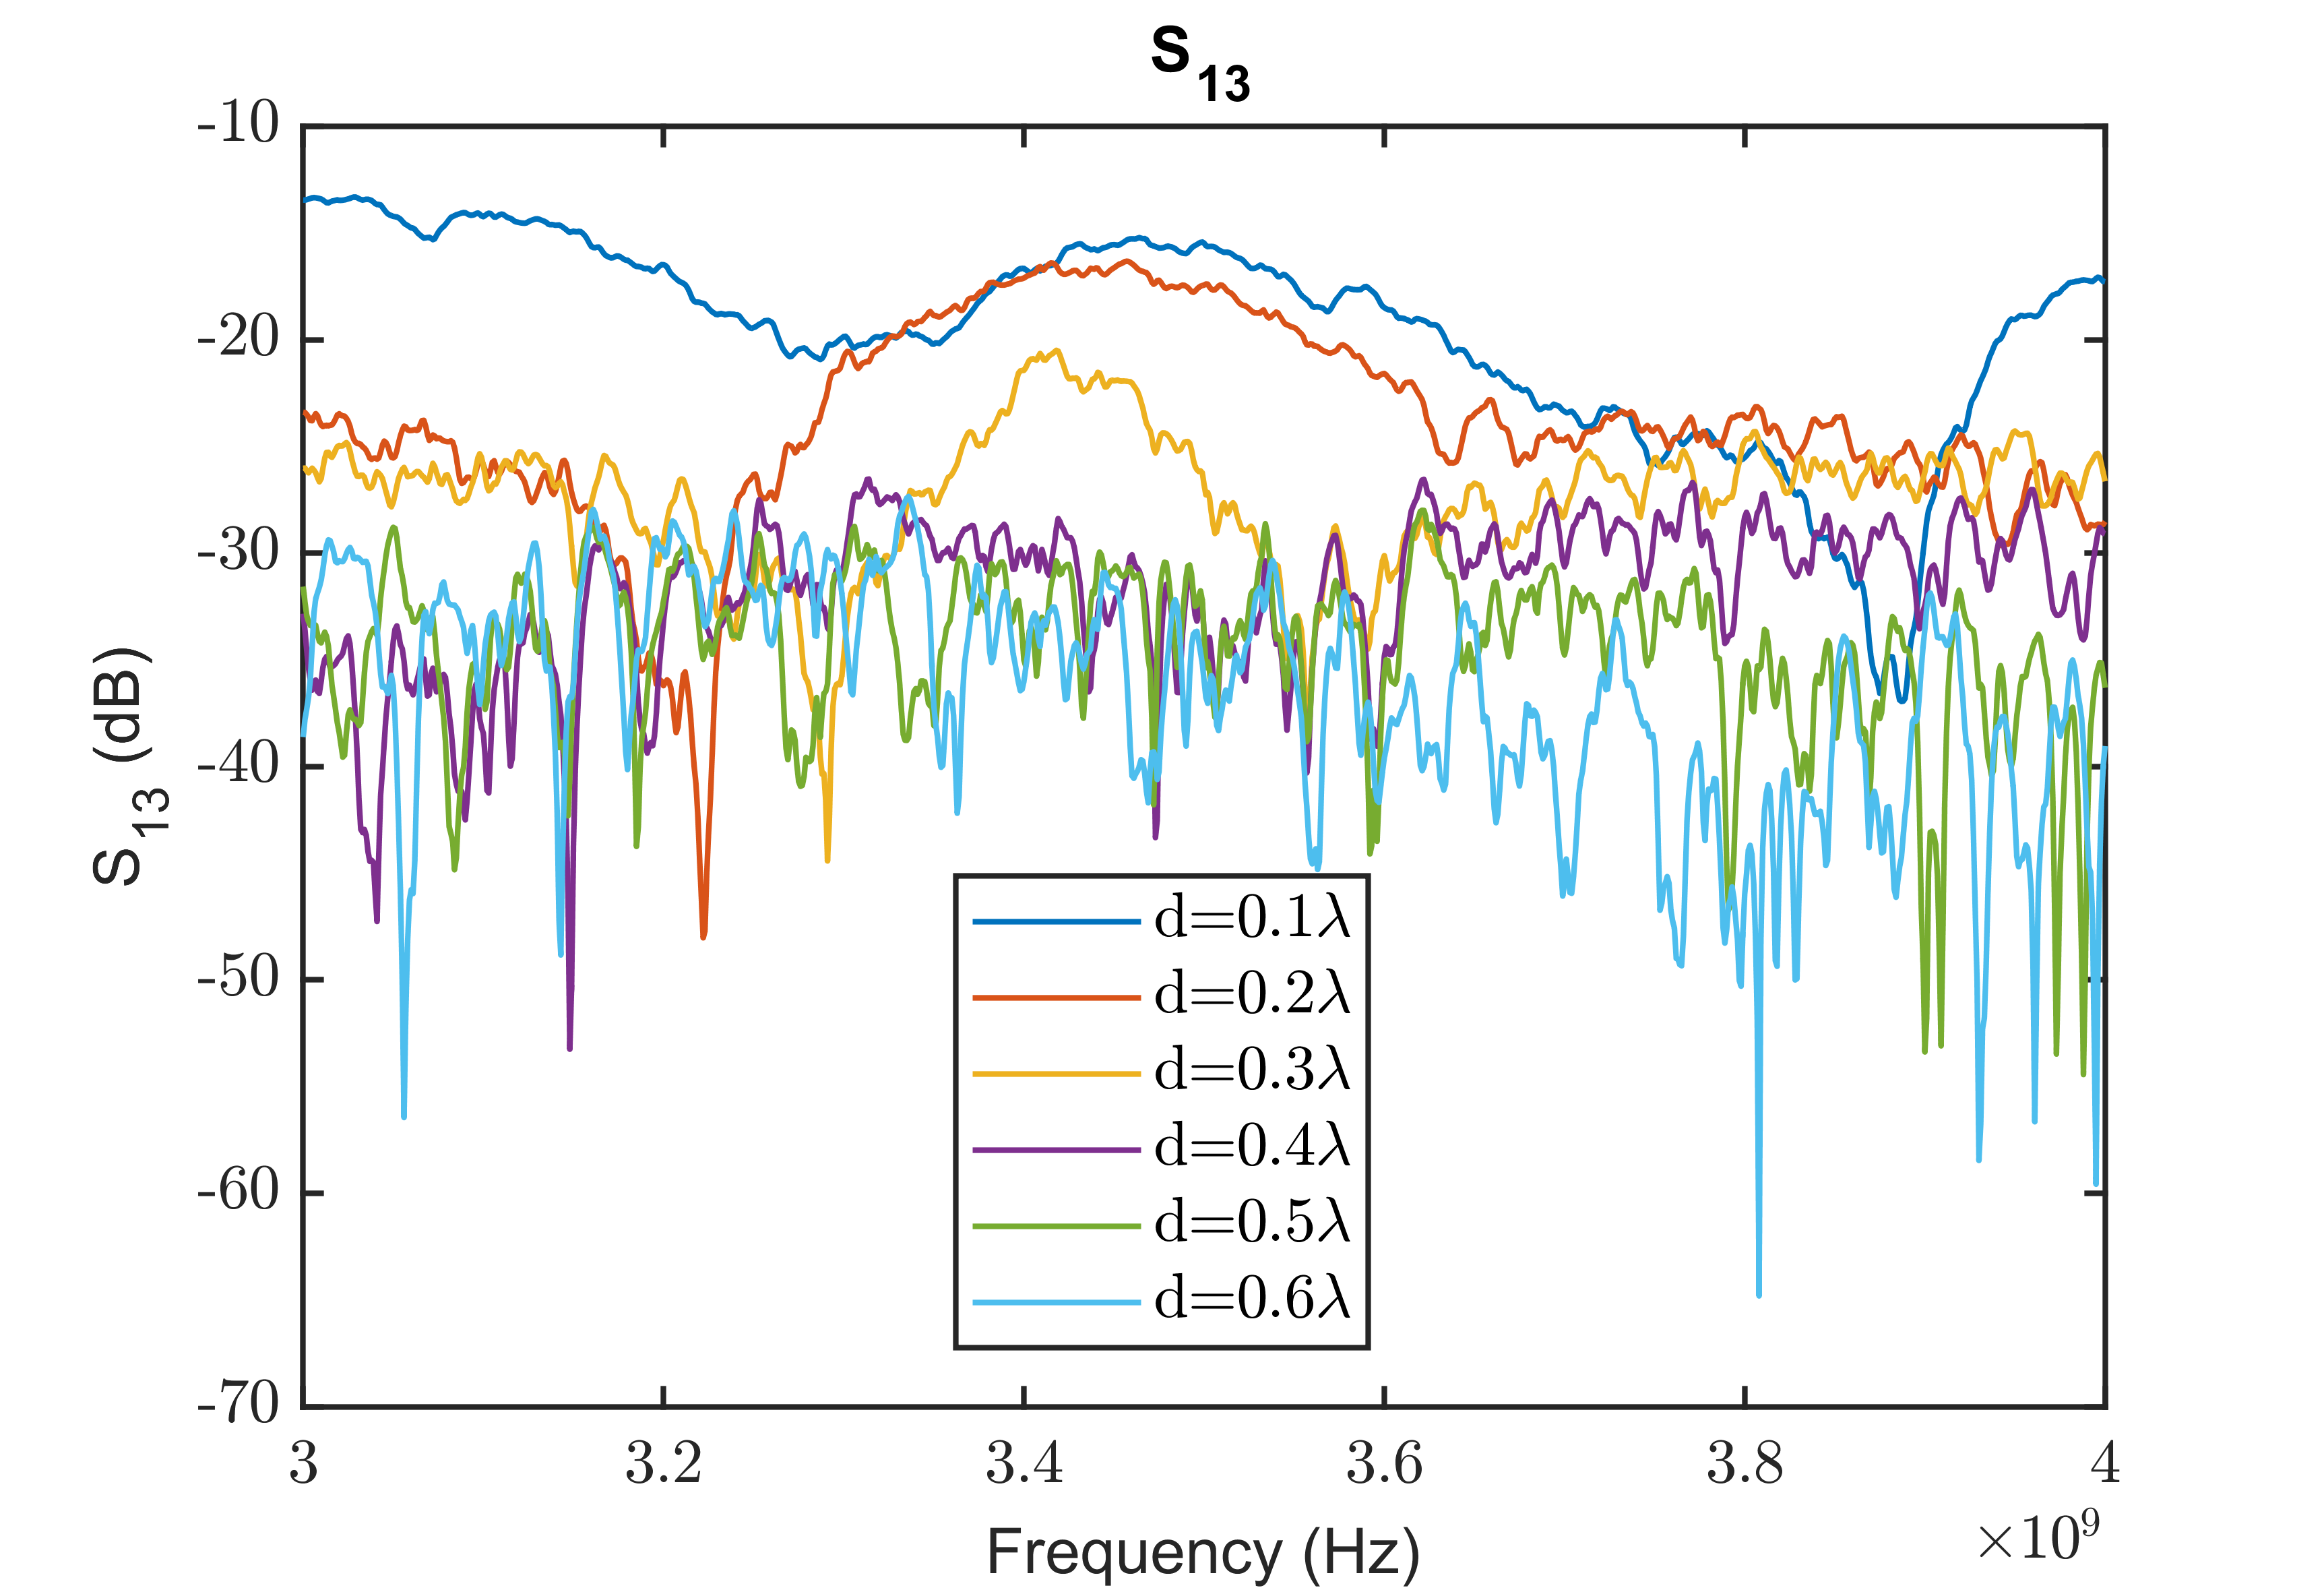
\includegraphics[scale = 0.5]{figures/measurement/antennas/spar_four_ant_s13.png}
	\caption{Measured $S_{13}$ with four antennas}
    \label{fig:chamber_four_ant_s13}
  \end{minipage}
  \hfill
  \begin{minipage}[b]{0.4\textwidth}
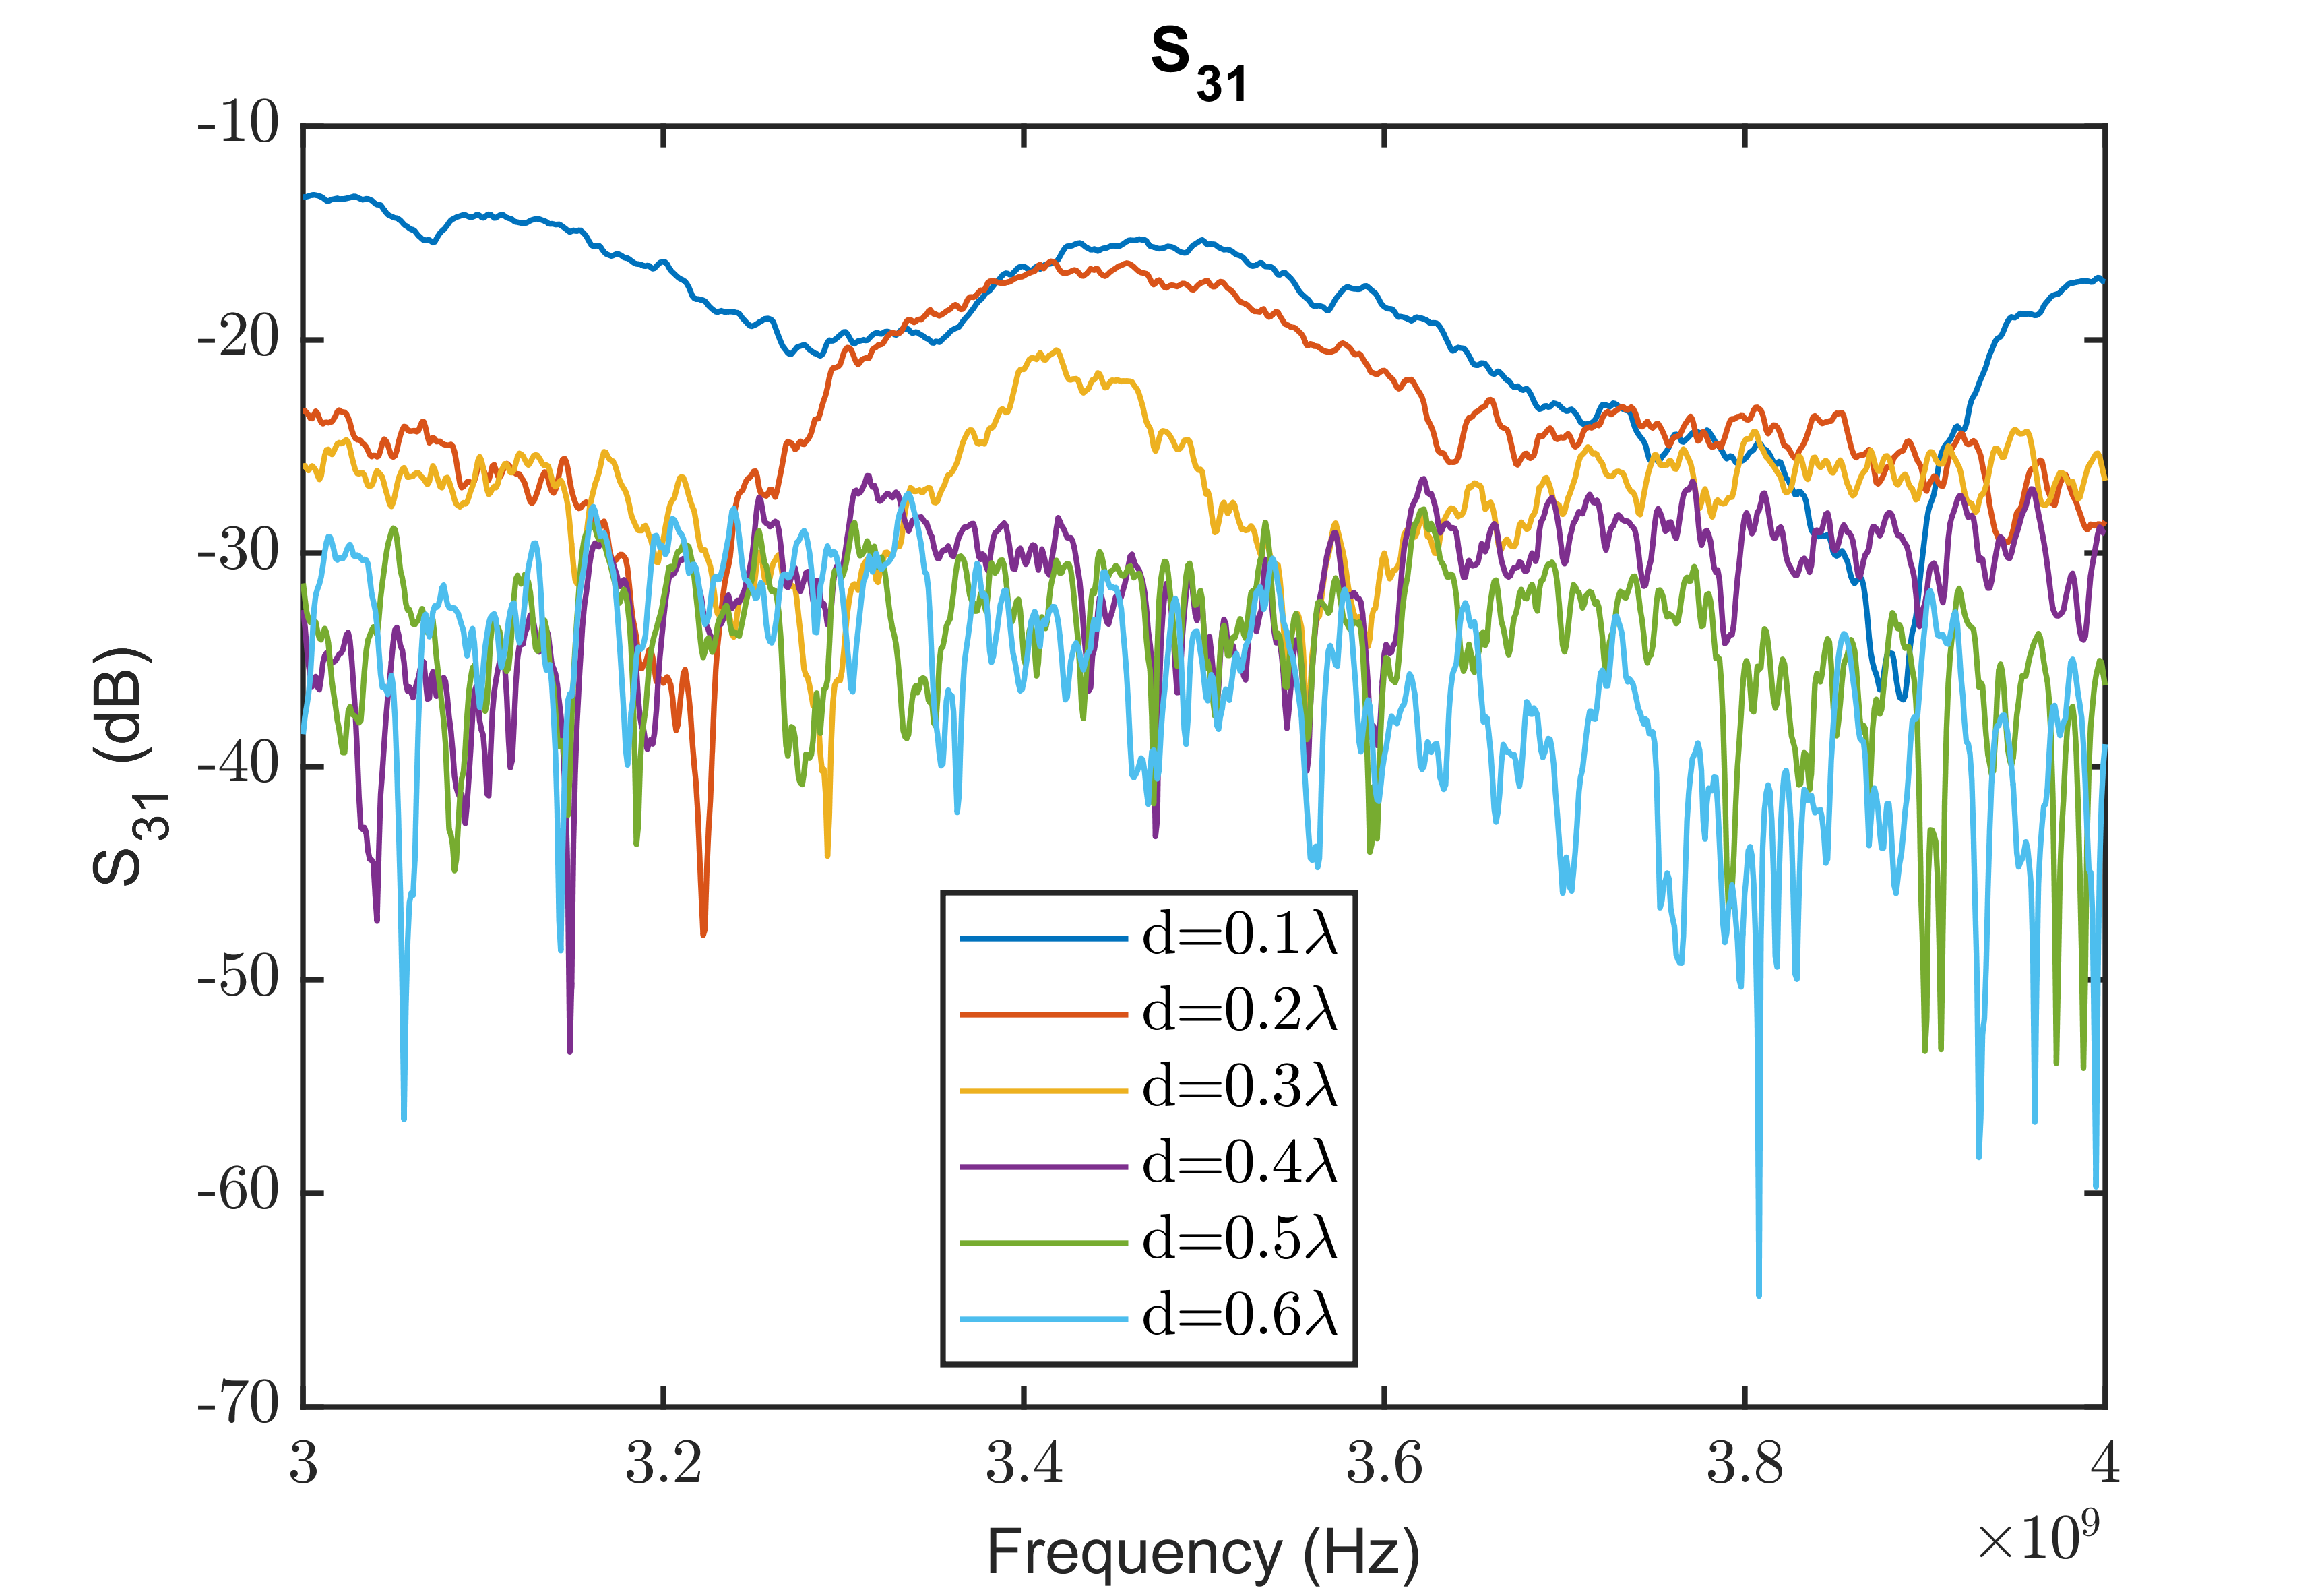
\includegraphics[scale = 0.5]{figures/measurement/antennas/spar_four_ant_s31.png}
\caption{Measured $S_{31}$ with four antennas}
    \label{fig:chamber_four_ant_s31}
  \end{minipage}
\end{figure}


\begin{figure}[H]
  \centering
  \begin{minipage}[b]{0.5\textwidth}
	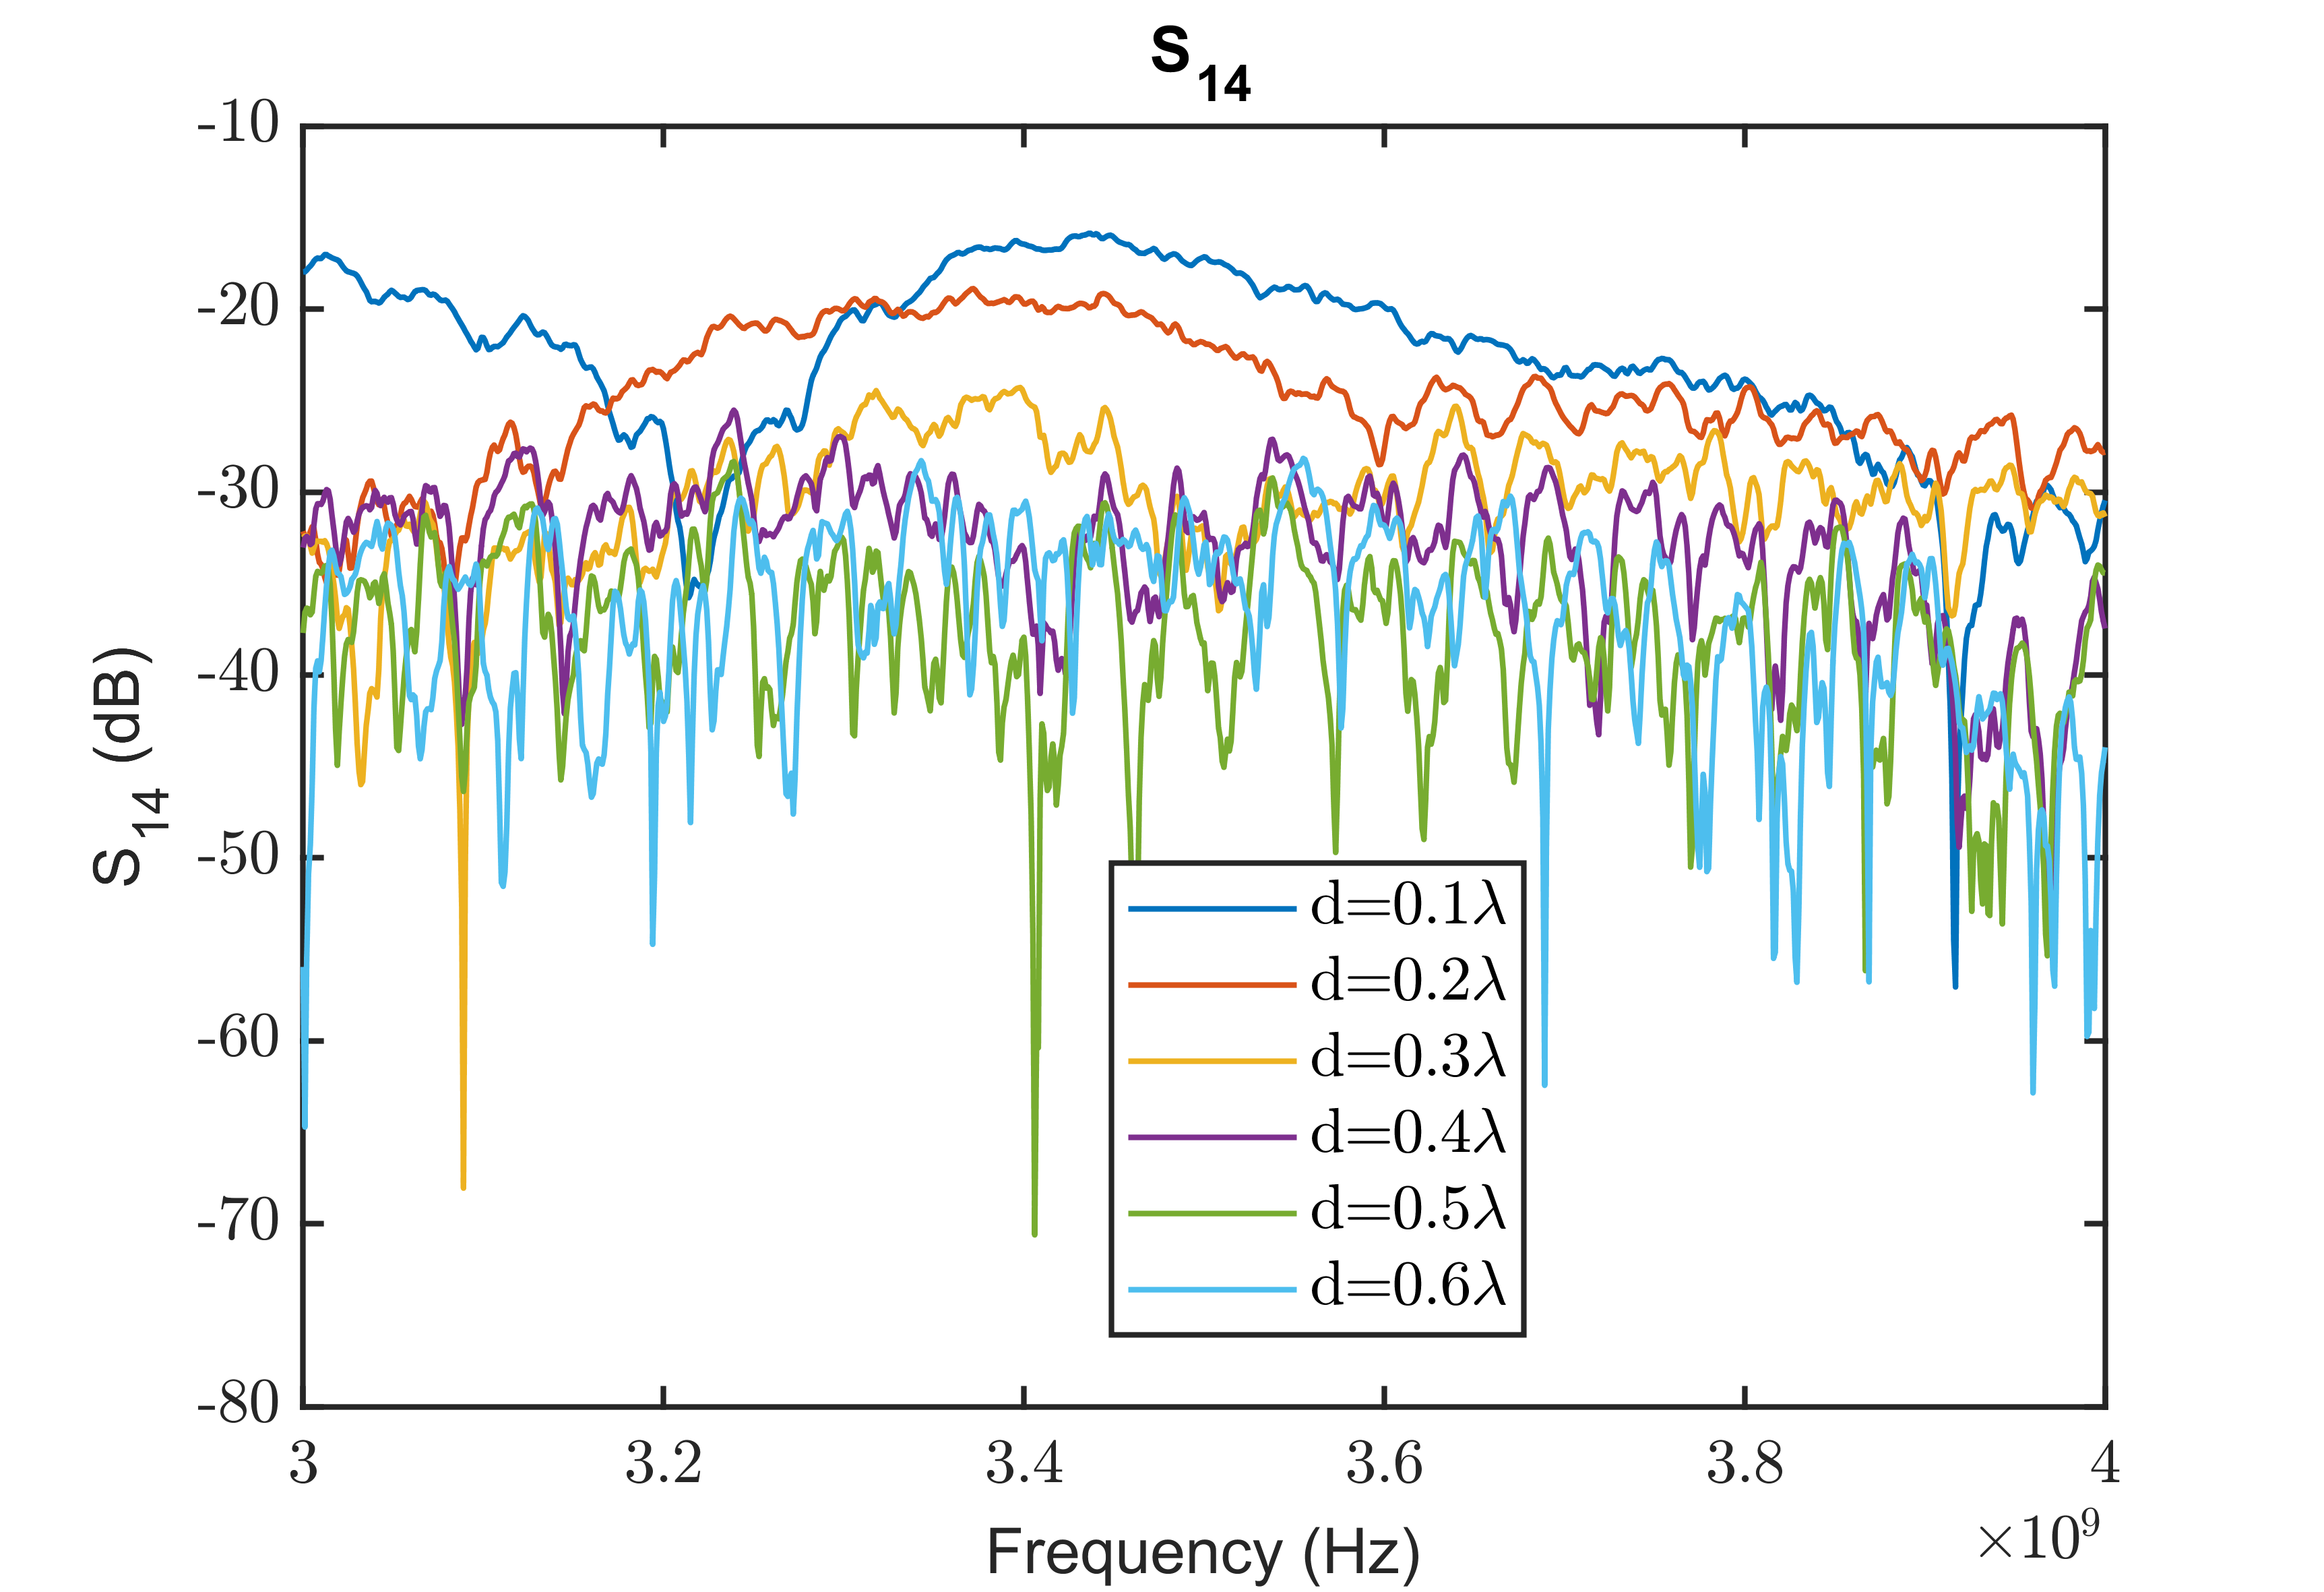
\includegraphics[scale = 0.5]{figures/measurement/antennas/spar_four_ant_s14.png}
	\caption{Measured $S_{14}$ with four antennas}
    \label{fig:chamber_four_ant_s14}
  \end{minipage}
  \hfill
  \begin{minipage}[b]{0.4\textwidth}
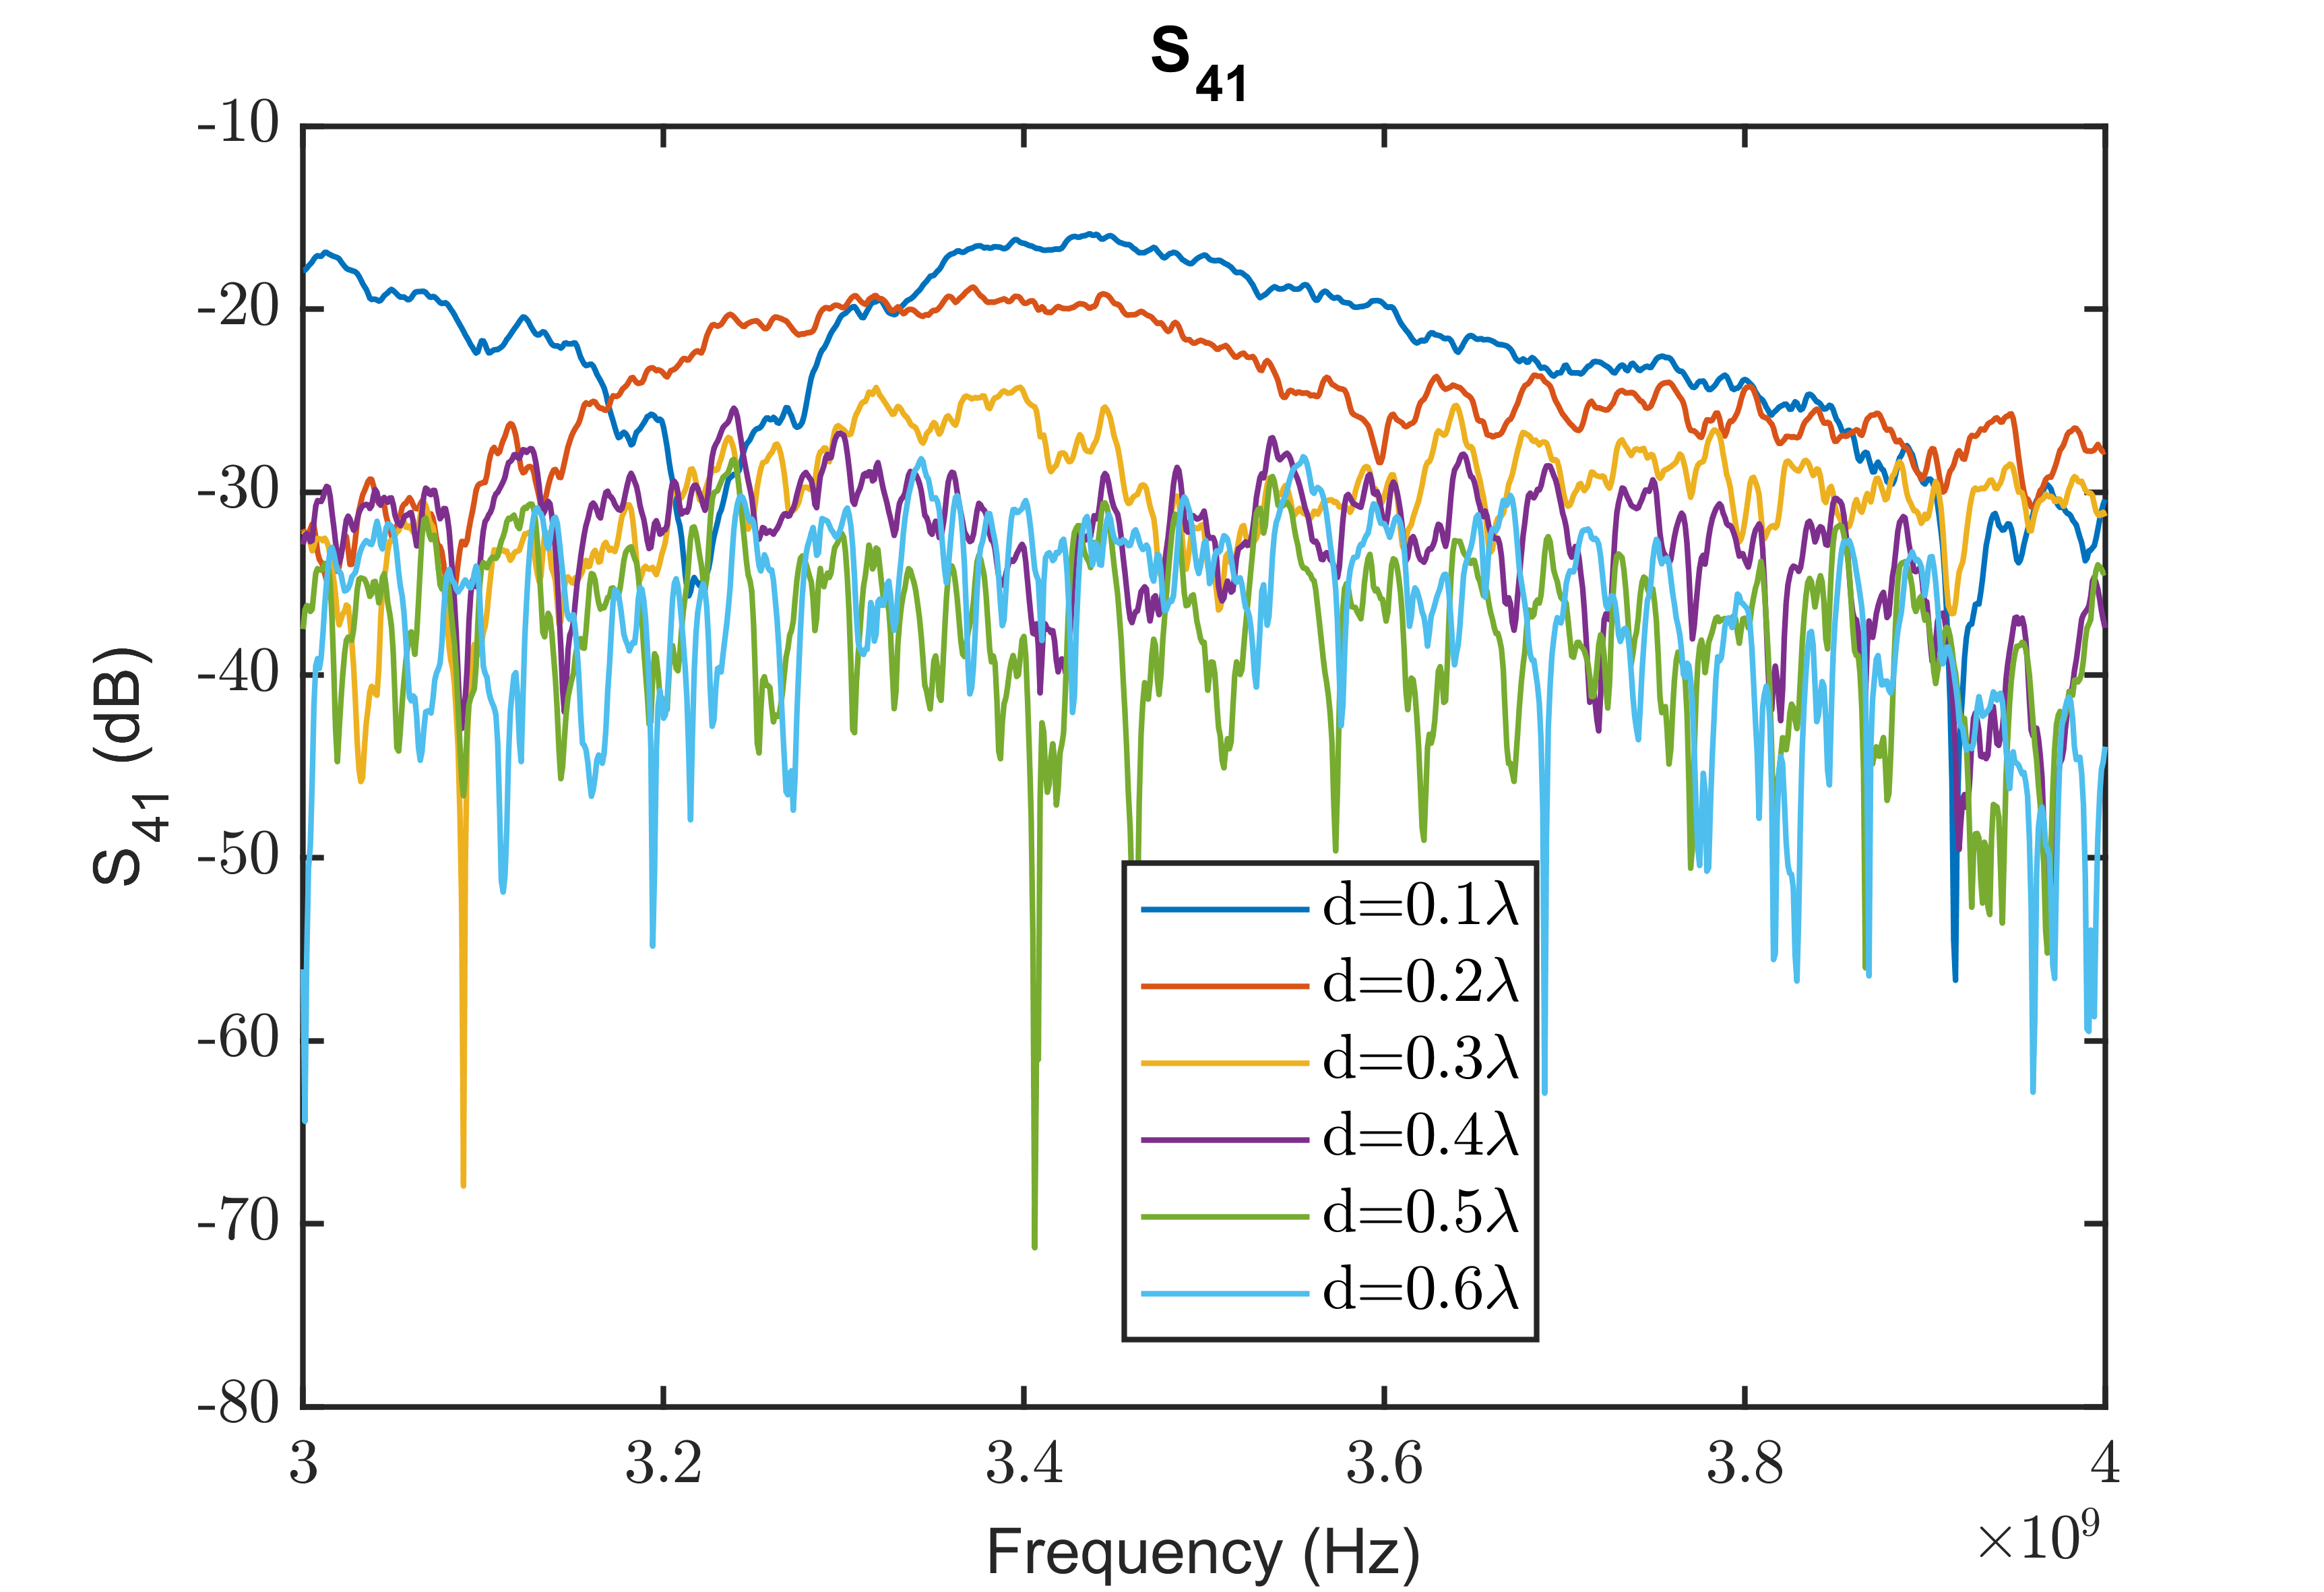
\includegraphics[scale = 0.5]{figures/measurement/antennas/spar_four_ant_s41.png}
\caption{Measured $S_{41}$ with four antennas}
    \label{fig:chamber_four_ant_s41}
  \end{minipage}
\end{figure}


\begin{figure}[H]
  \centering
  \begin{minipage}[b]{0.5\textwidth}
	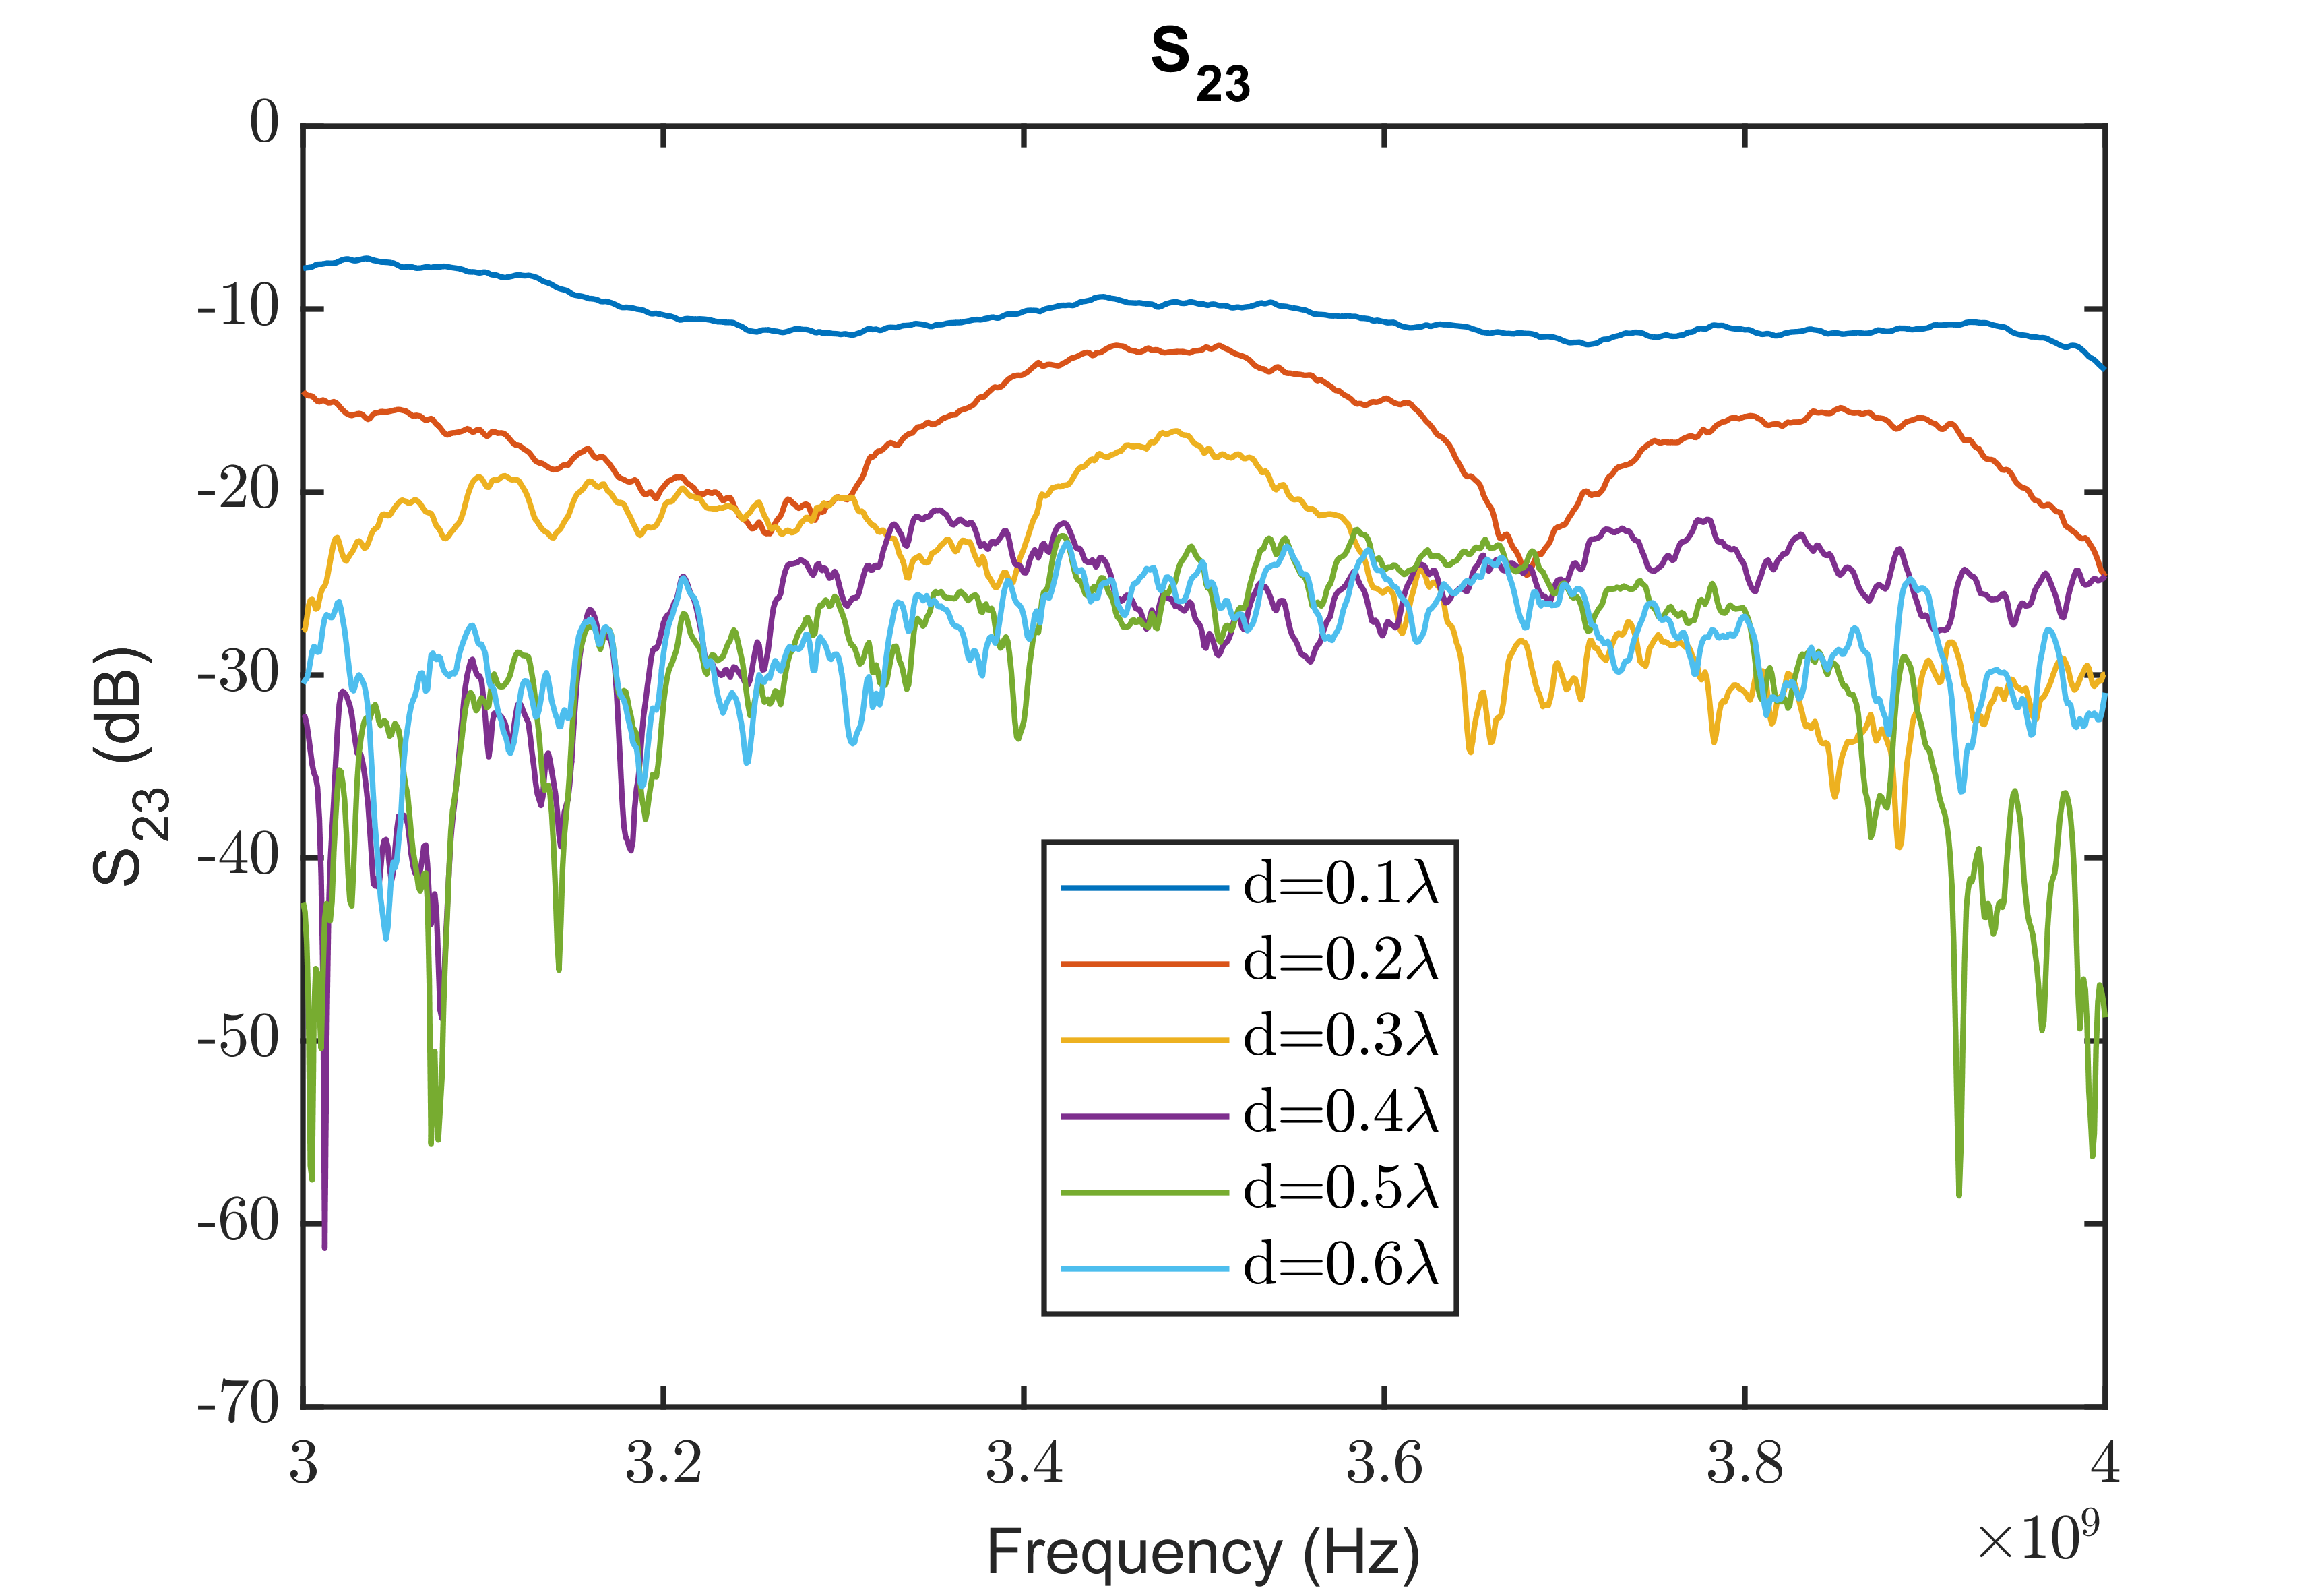
\includegraphics[scale = 0.5]{figures/measurement/antennas/spar_four_ant_s23.png}
	\caption{Measured $S_{23}$ with four antennas}
    \label{fig:chamber_four_ant_s23}
  \end{minipage}
  \hfill
  \begin{minipage}[b]{0.4\textwidth}
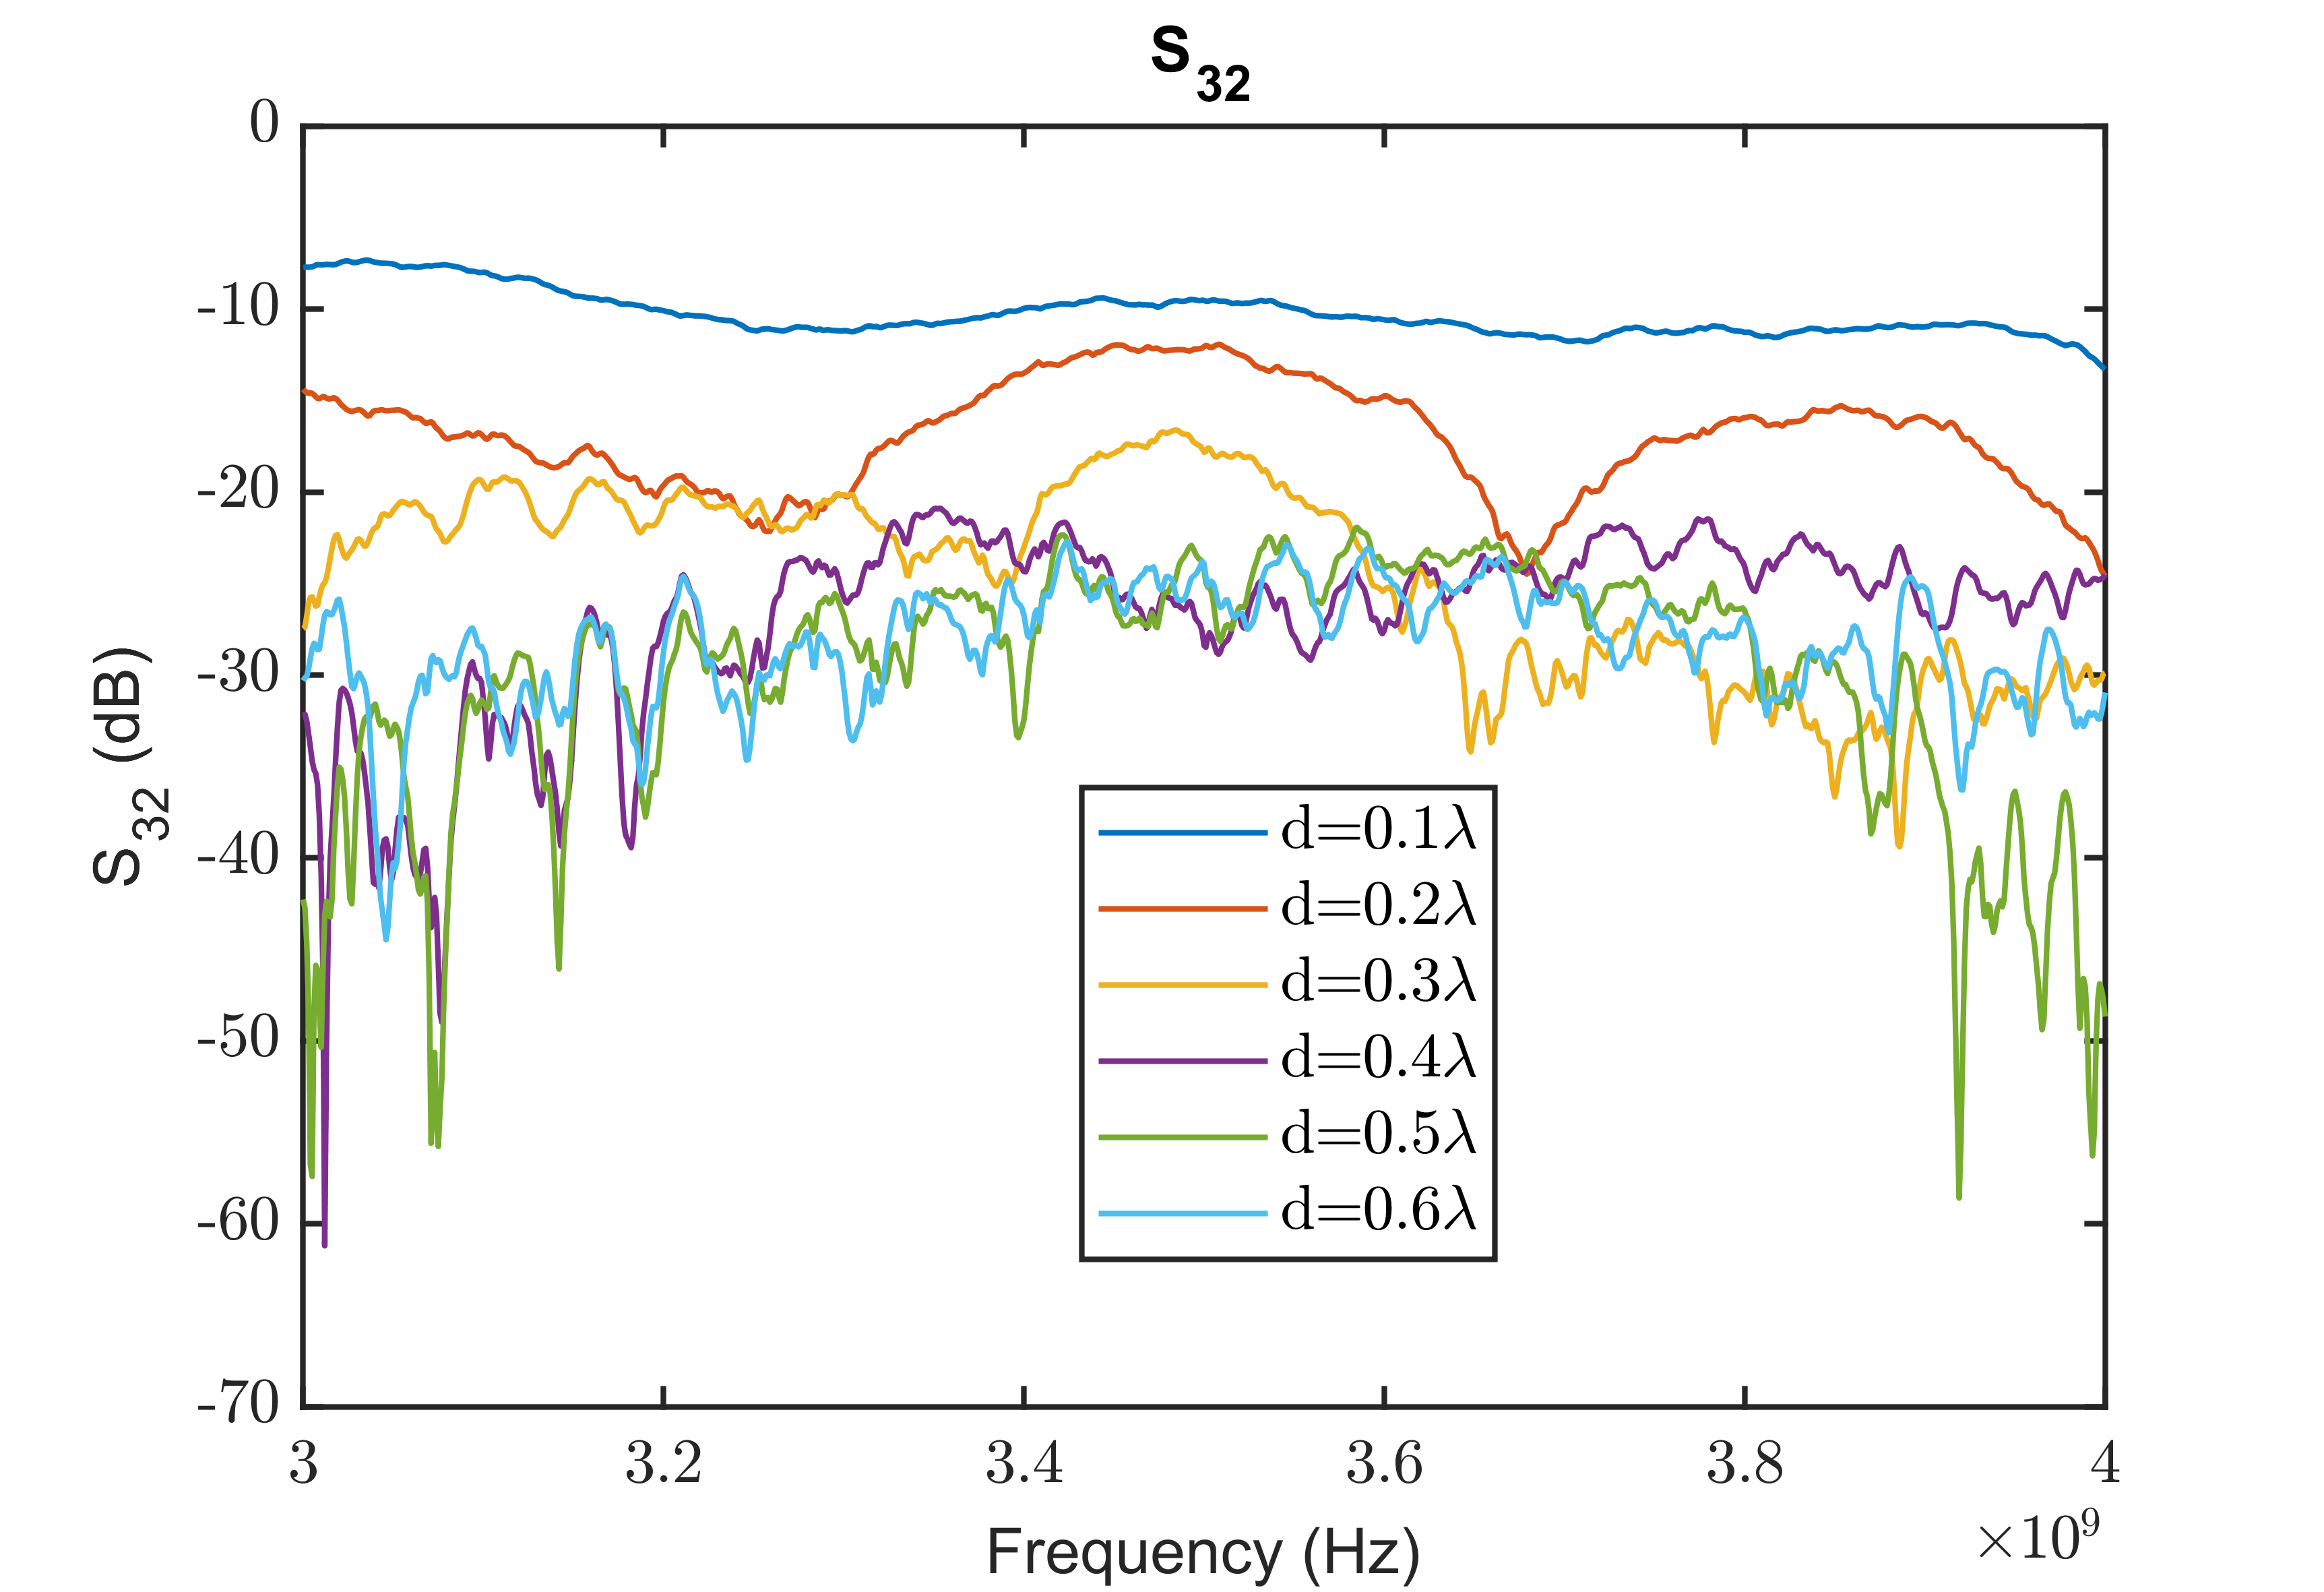
\includegraphics[scale = 0.5]{figures/measurement/antennas/spar_four_ant_s32.png}
\caption{Measured $S_{32}$ with four antennas}
    \label{fig:chamber_four_ant_s32}
  \end{minipage}
\end{figure}





\begin{figure}[H]
\centering 
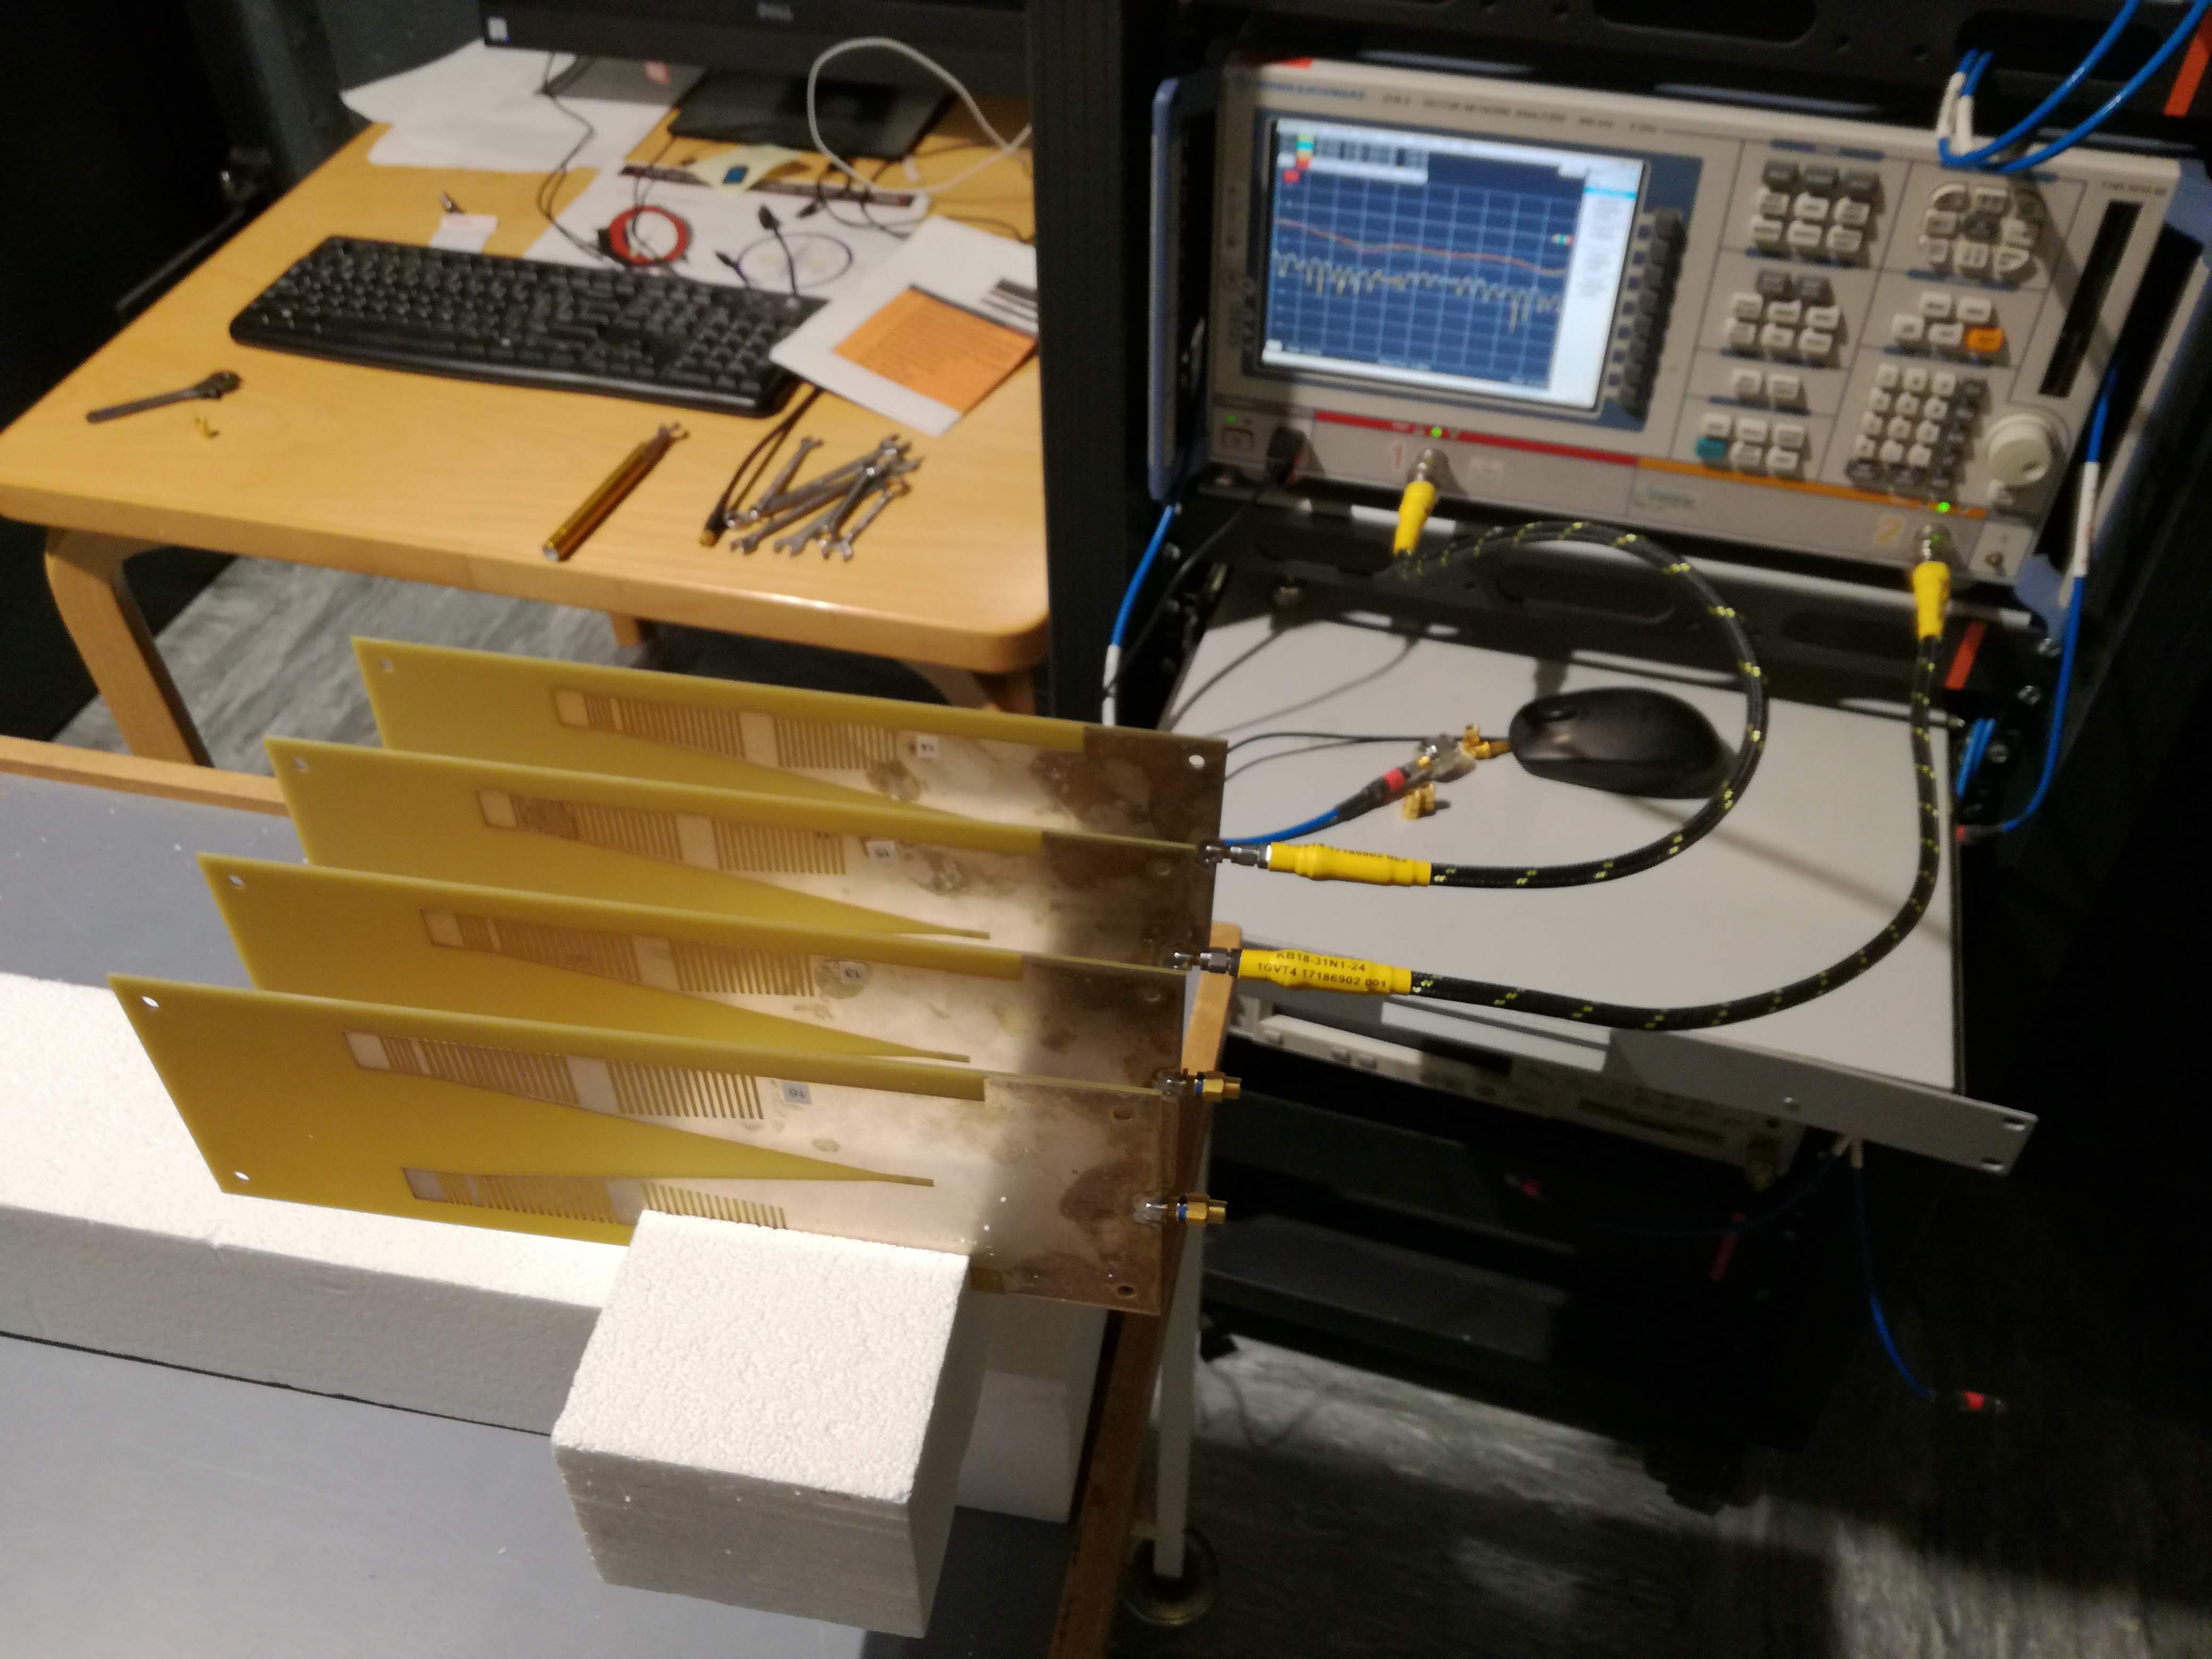
\includegraphics[scale = 0.08]{figures/measurement/antennas/spar_meas.jpg}
\caption{Measurement of S-parameters using four antennas. The measurement using one and two antennas has been done at the same way. The unused antennas are terminated to $50\Omega$}
\label{fig:spar_meas}
\end{figure} 


%%%%%%%%%%%%%%%%%%%%%%%%%%%%%%%%%%%%%%%%%%%%%%%%%%%%%%%%%%%%%%%%%%%%%%%%%%%%%%%%%%%%%%%%%%%%%%%%%%%%%%%%%%
\section{Single element four antennas}
In this section the farfield of a single element in a array with 4 antennas is measured. It is expected that the first and fourth element has a radiation pattern equal to each other and that second and the third is also equal to each other. It is seen to be somewhat true in figure \ref{fig:chamber_four_ant_ff_1} to \ref{fig:chamber_four_ant_ff_4} thou variations is seen.     


\begin{figure}[H]
\centering 
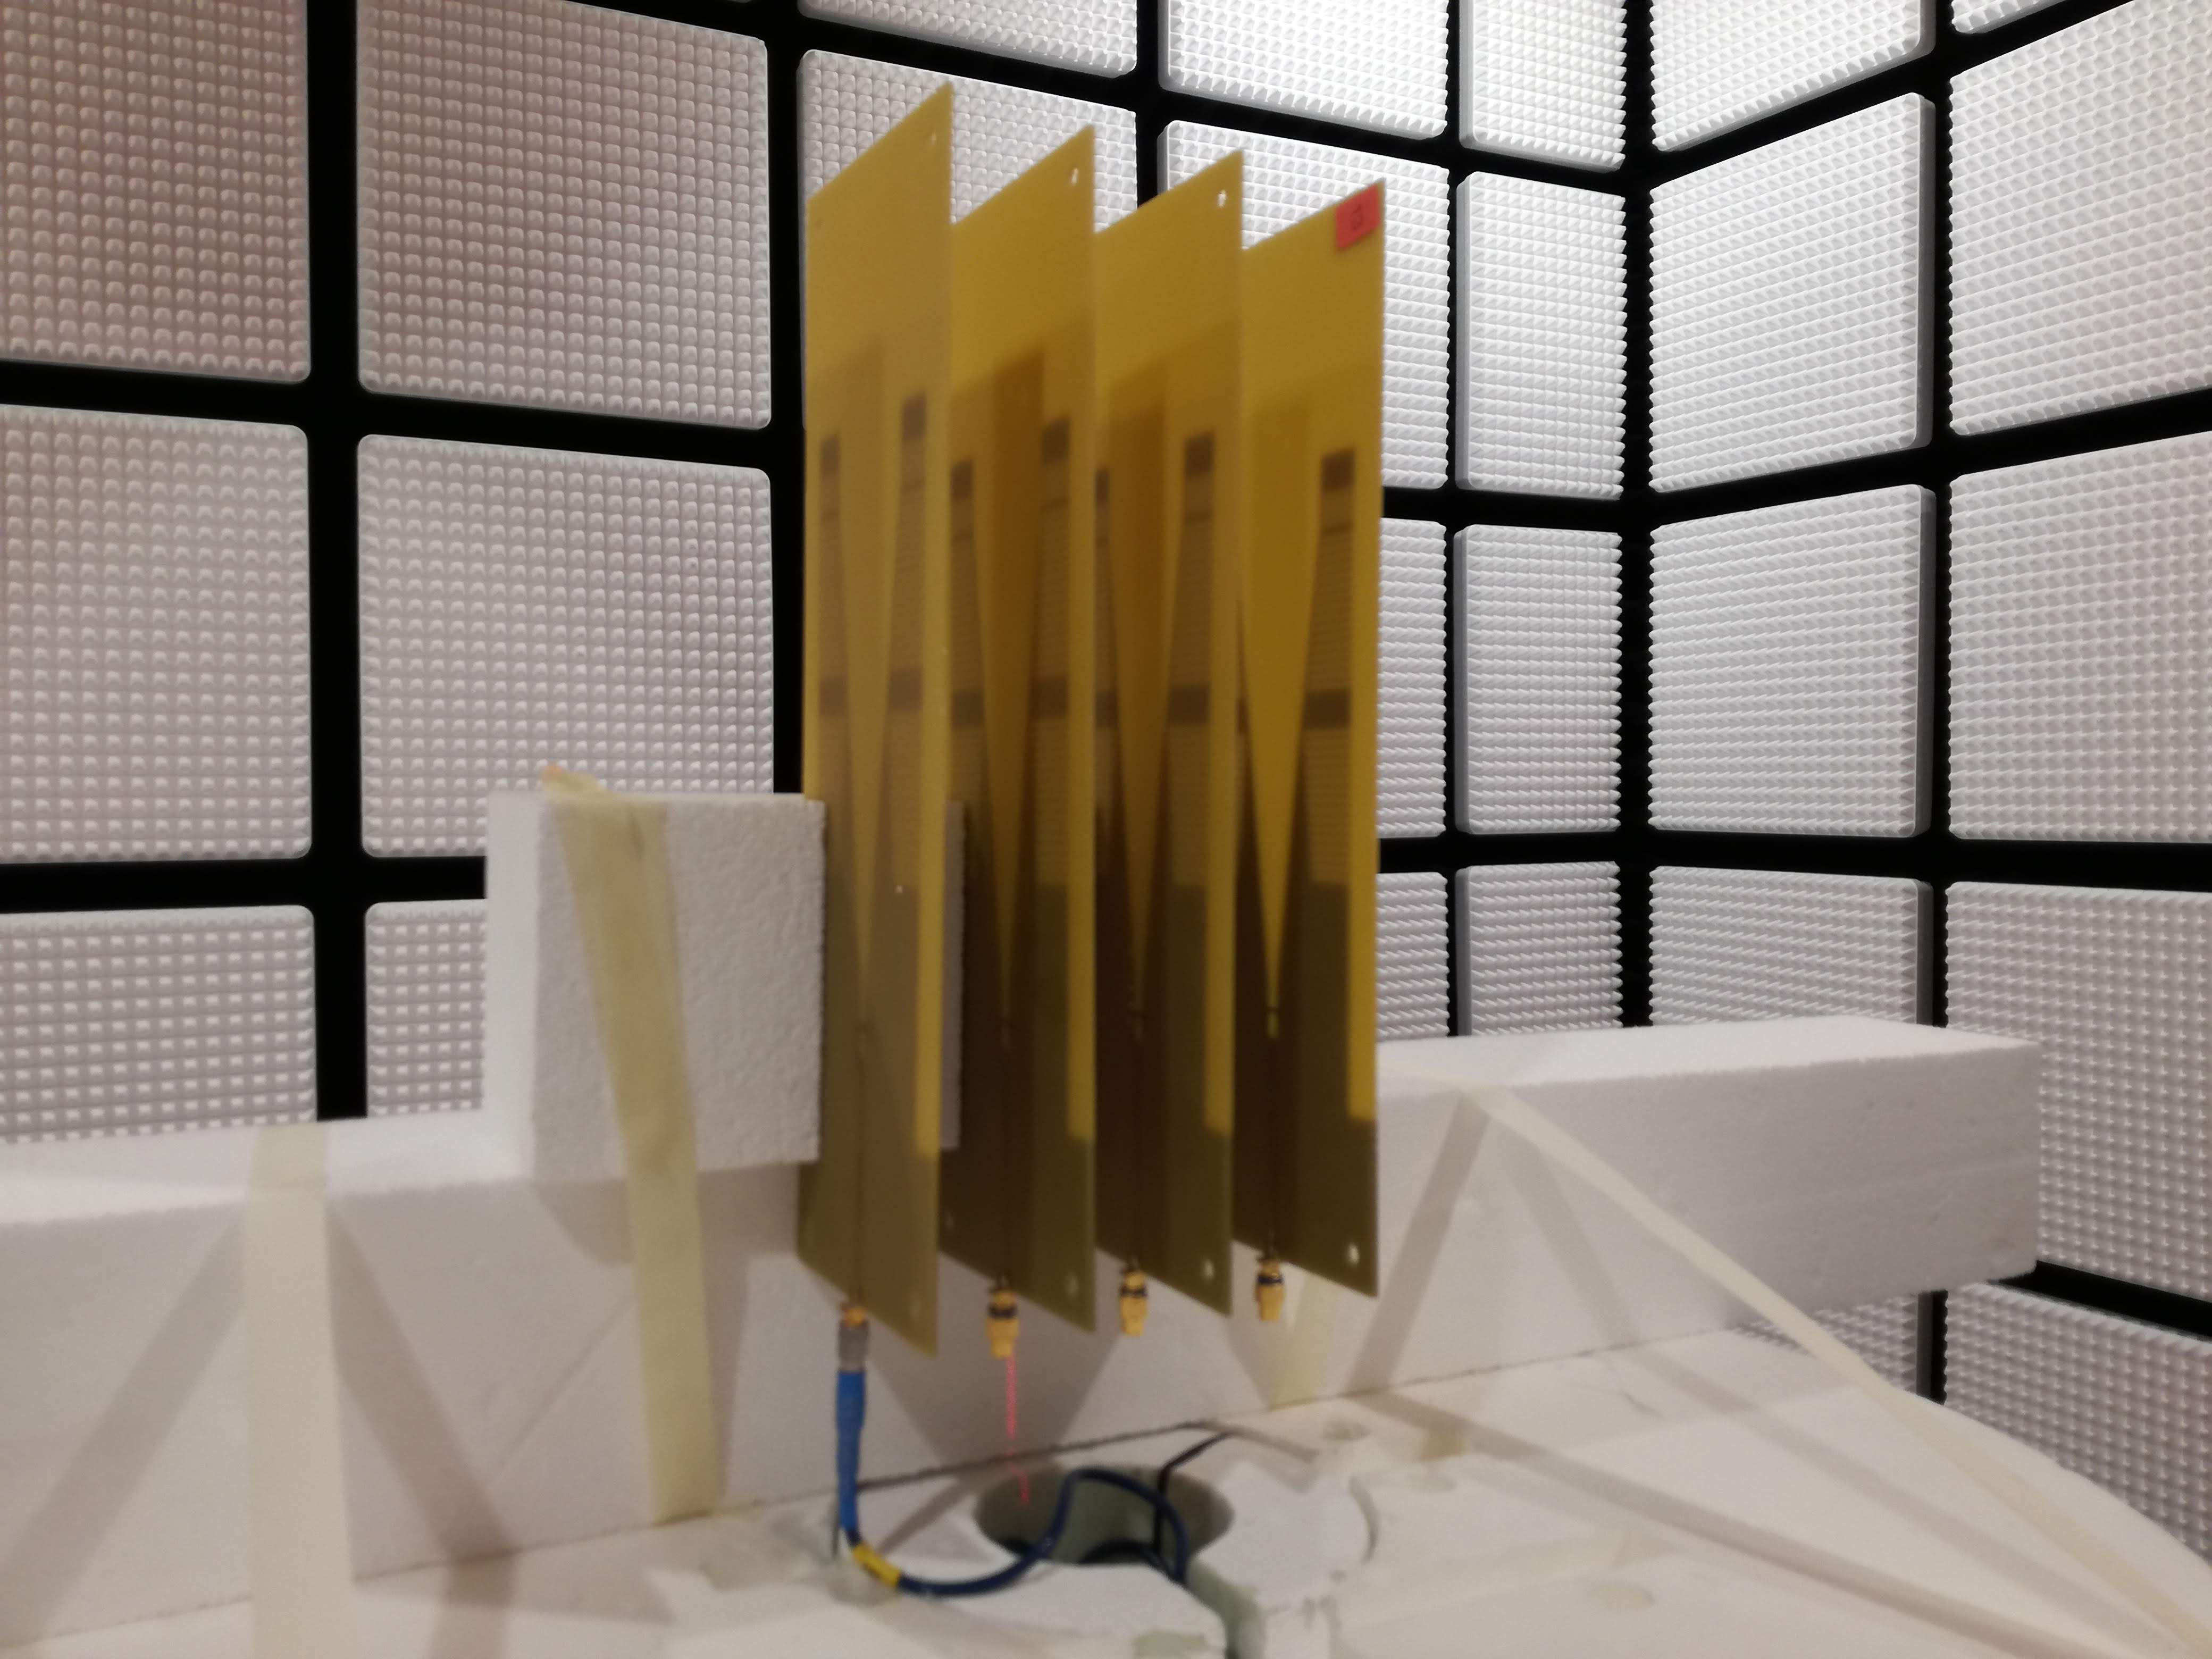
\includegraphics[scale = 0.05]{figures/measurement/antennas/single_element_array.jpg}
\caption{Measurement of a single antenna in a 4 element array. The unused antennas is terminated to $50\Omega$. For every measurement the cable is mounted on another antenna and the load is shifted.}
\label{fig:chamber_four_ant0}
\end{figure} 


\begin{figure}[H]
  \centering
  \begin{minipage}[b]{0.5\textwidth}
	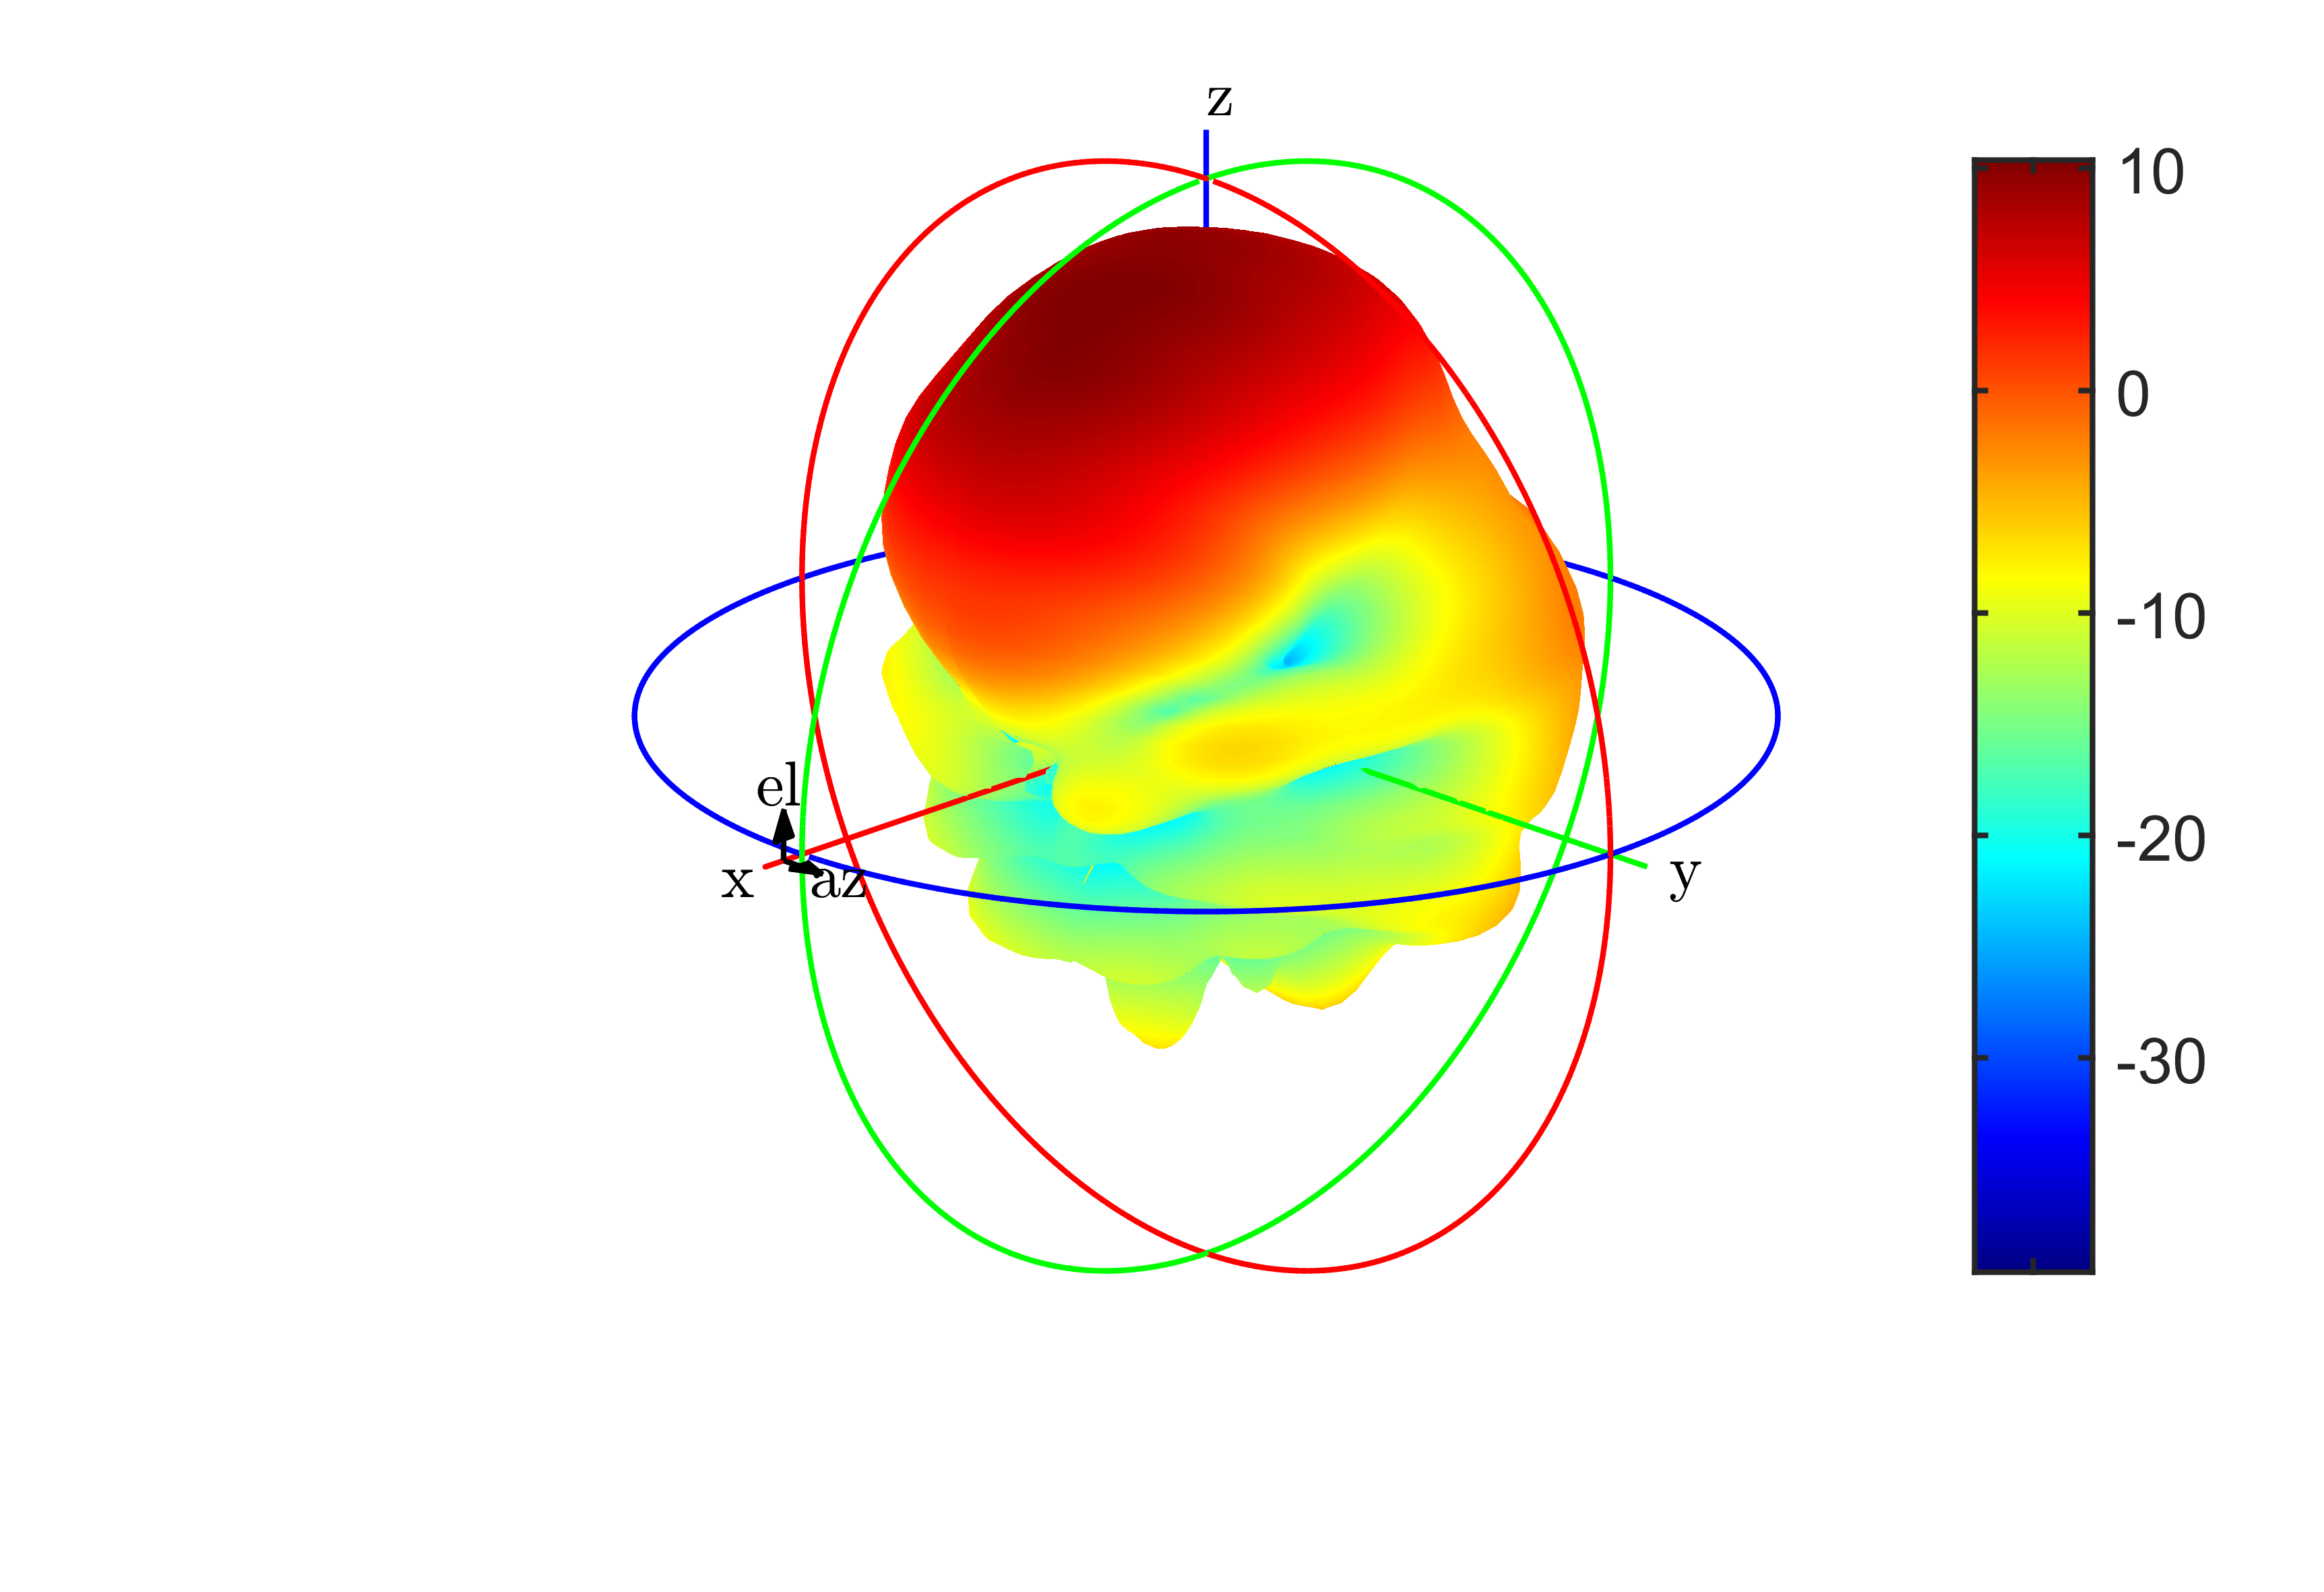
\includegraphics[scale = 0.5]{figures/measurement/antennas/1st_element_4_array.png}
	\caption{Farfield first element in the four element array. Maximum gain is 10.4dB}
    \label{fig:chamber_four_ant_ff_1}
  \end{minipage}
  \hfill
  \begin{minipage}[b]{0.4\textwidth}
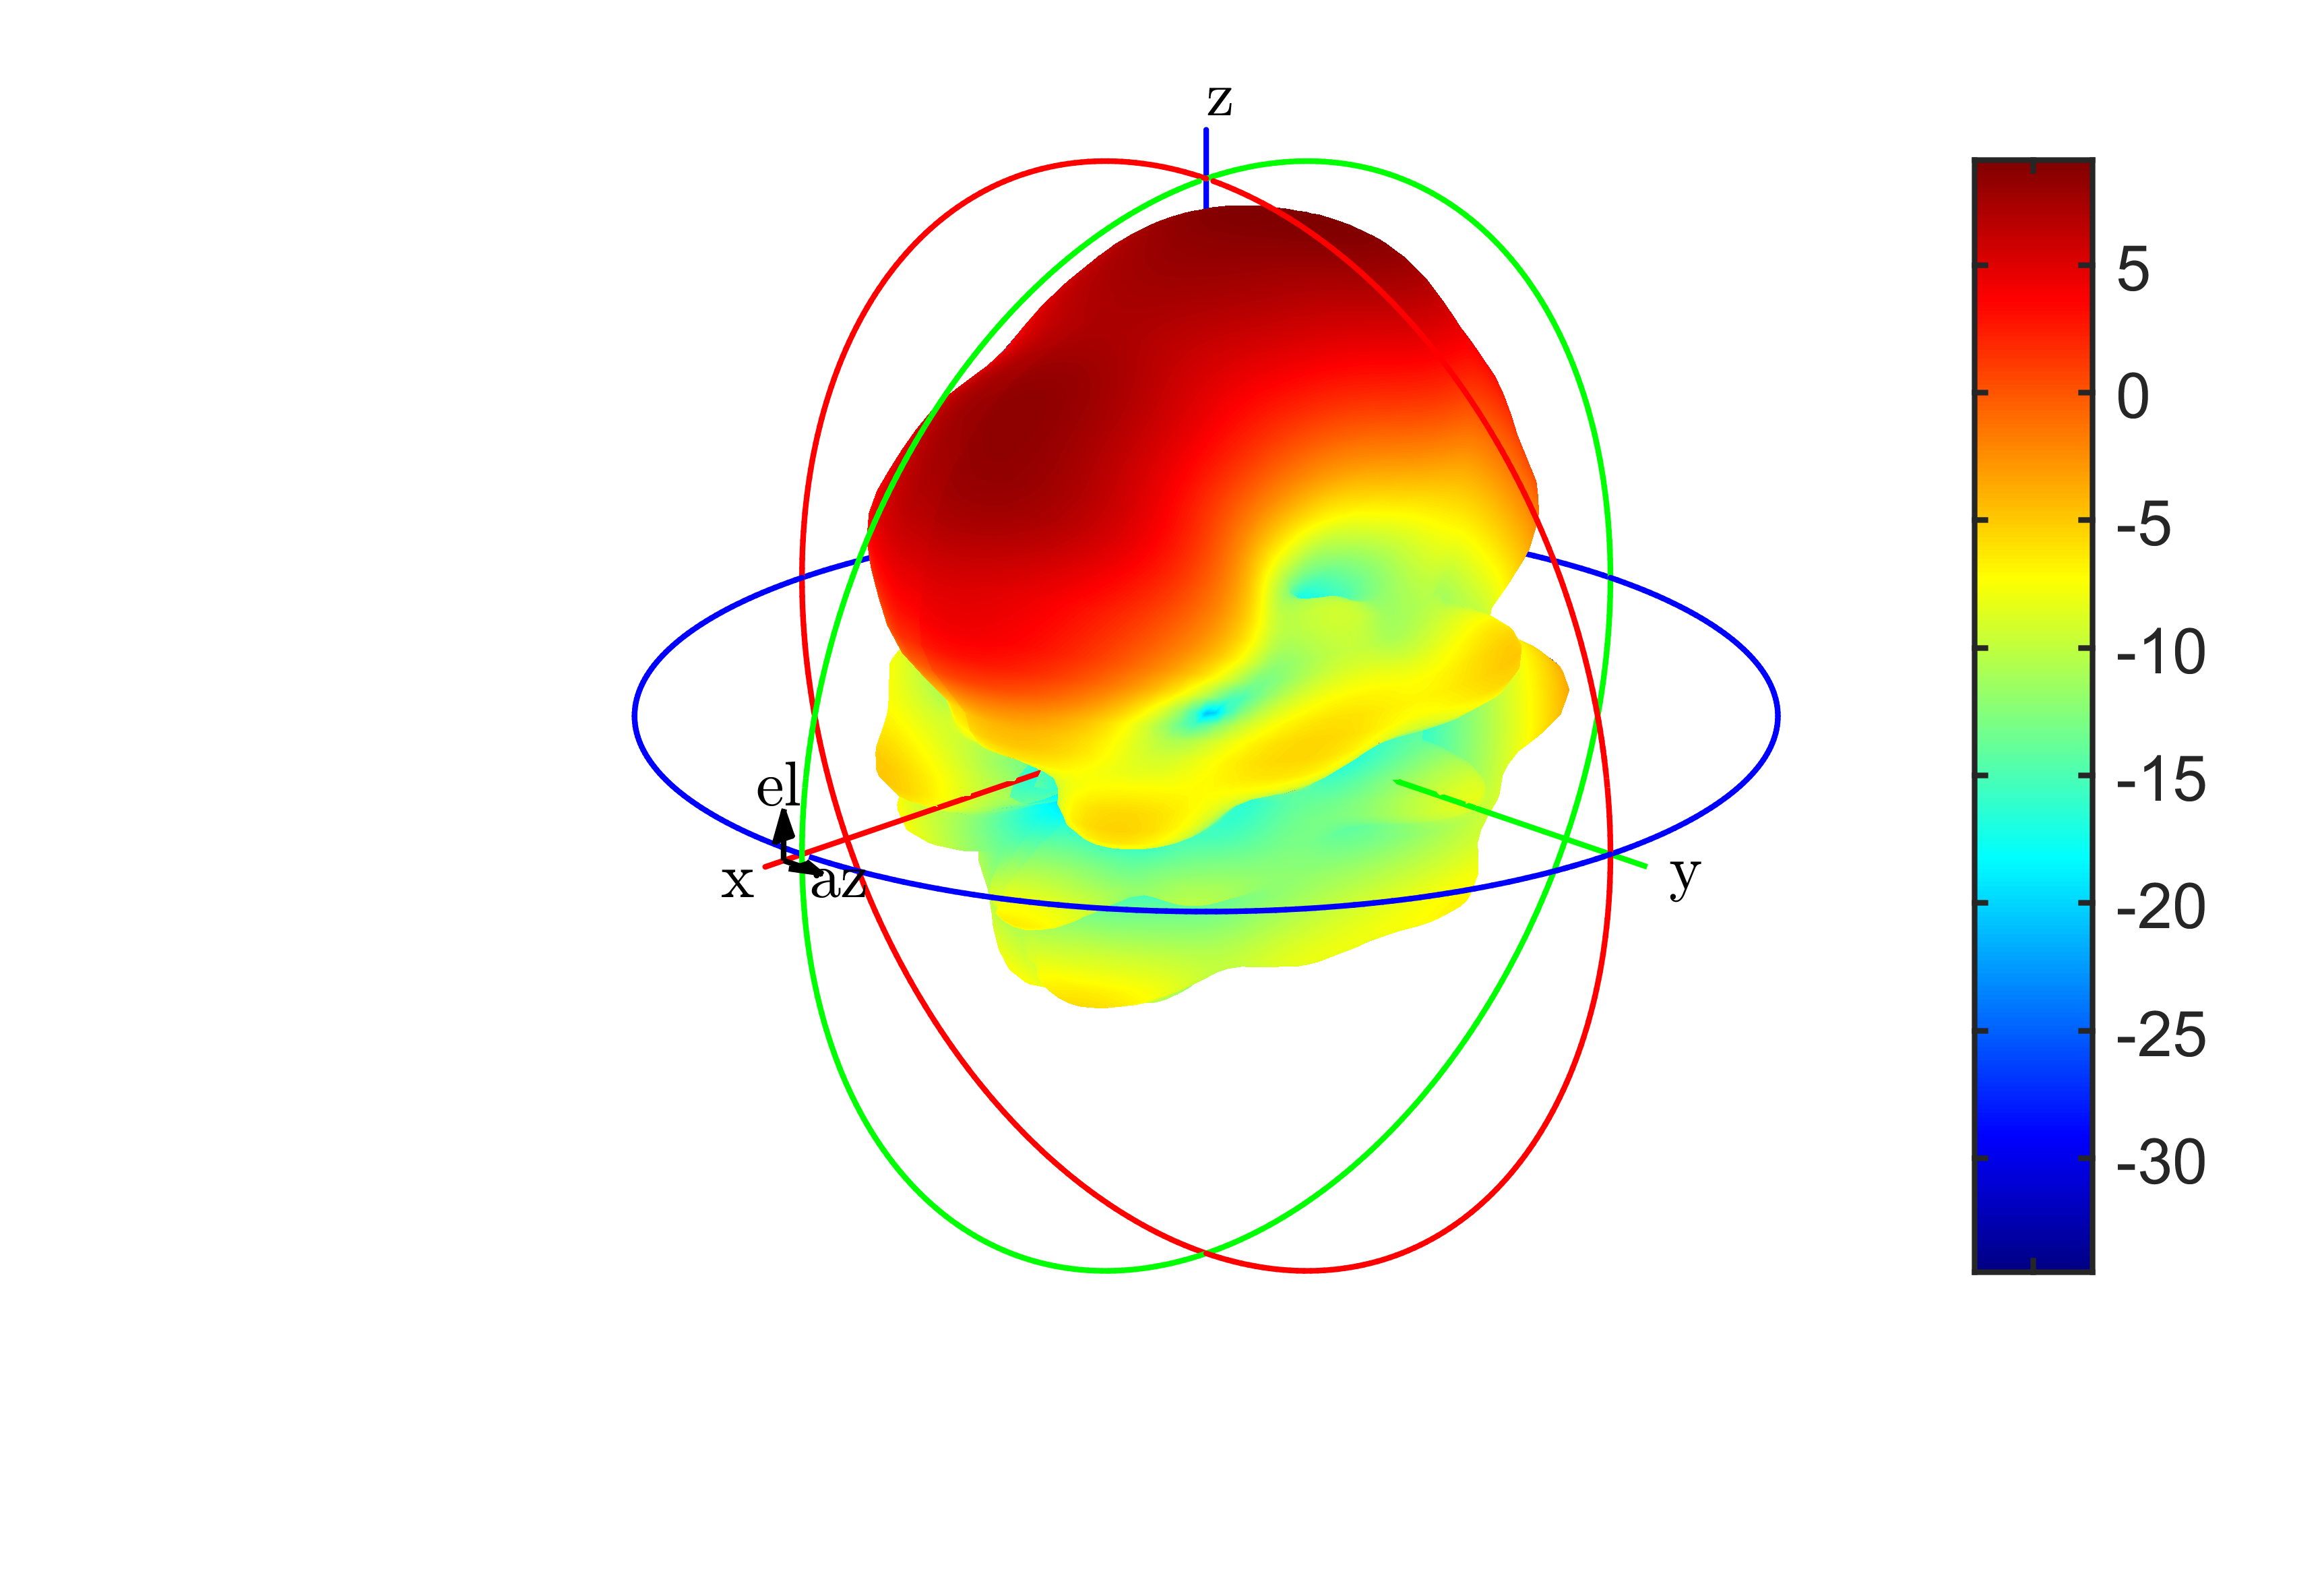
\includegraphics[scale = 0.5]{figures/measurement/antennas/2nd_element_4_array.png}
\caption{Farfield second element in the four element array. Maximum gain is 9.1dB}
    \label{fig:chamber_four_ant_ff:2}
  \end{minipage}
\end{figure}


\begin{figure}[H]
  \centering
  \begin{minipage}[b]{0.5\textwidth}
	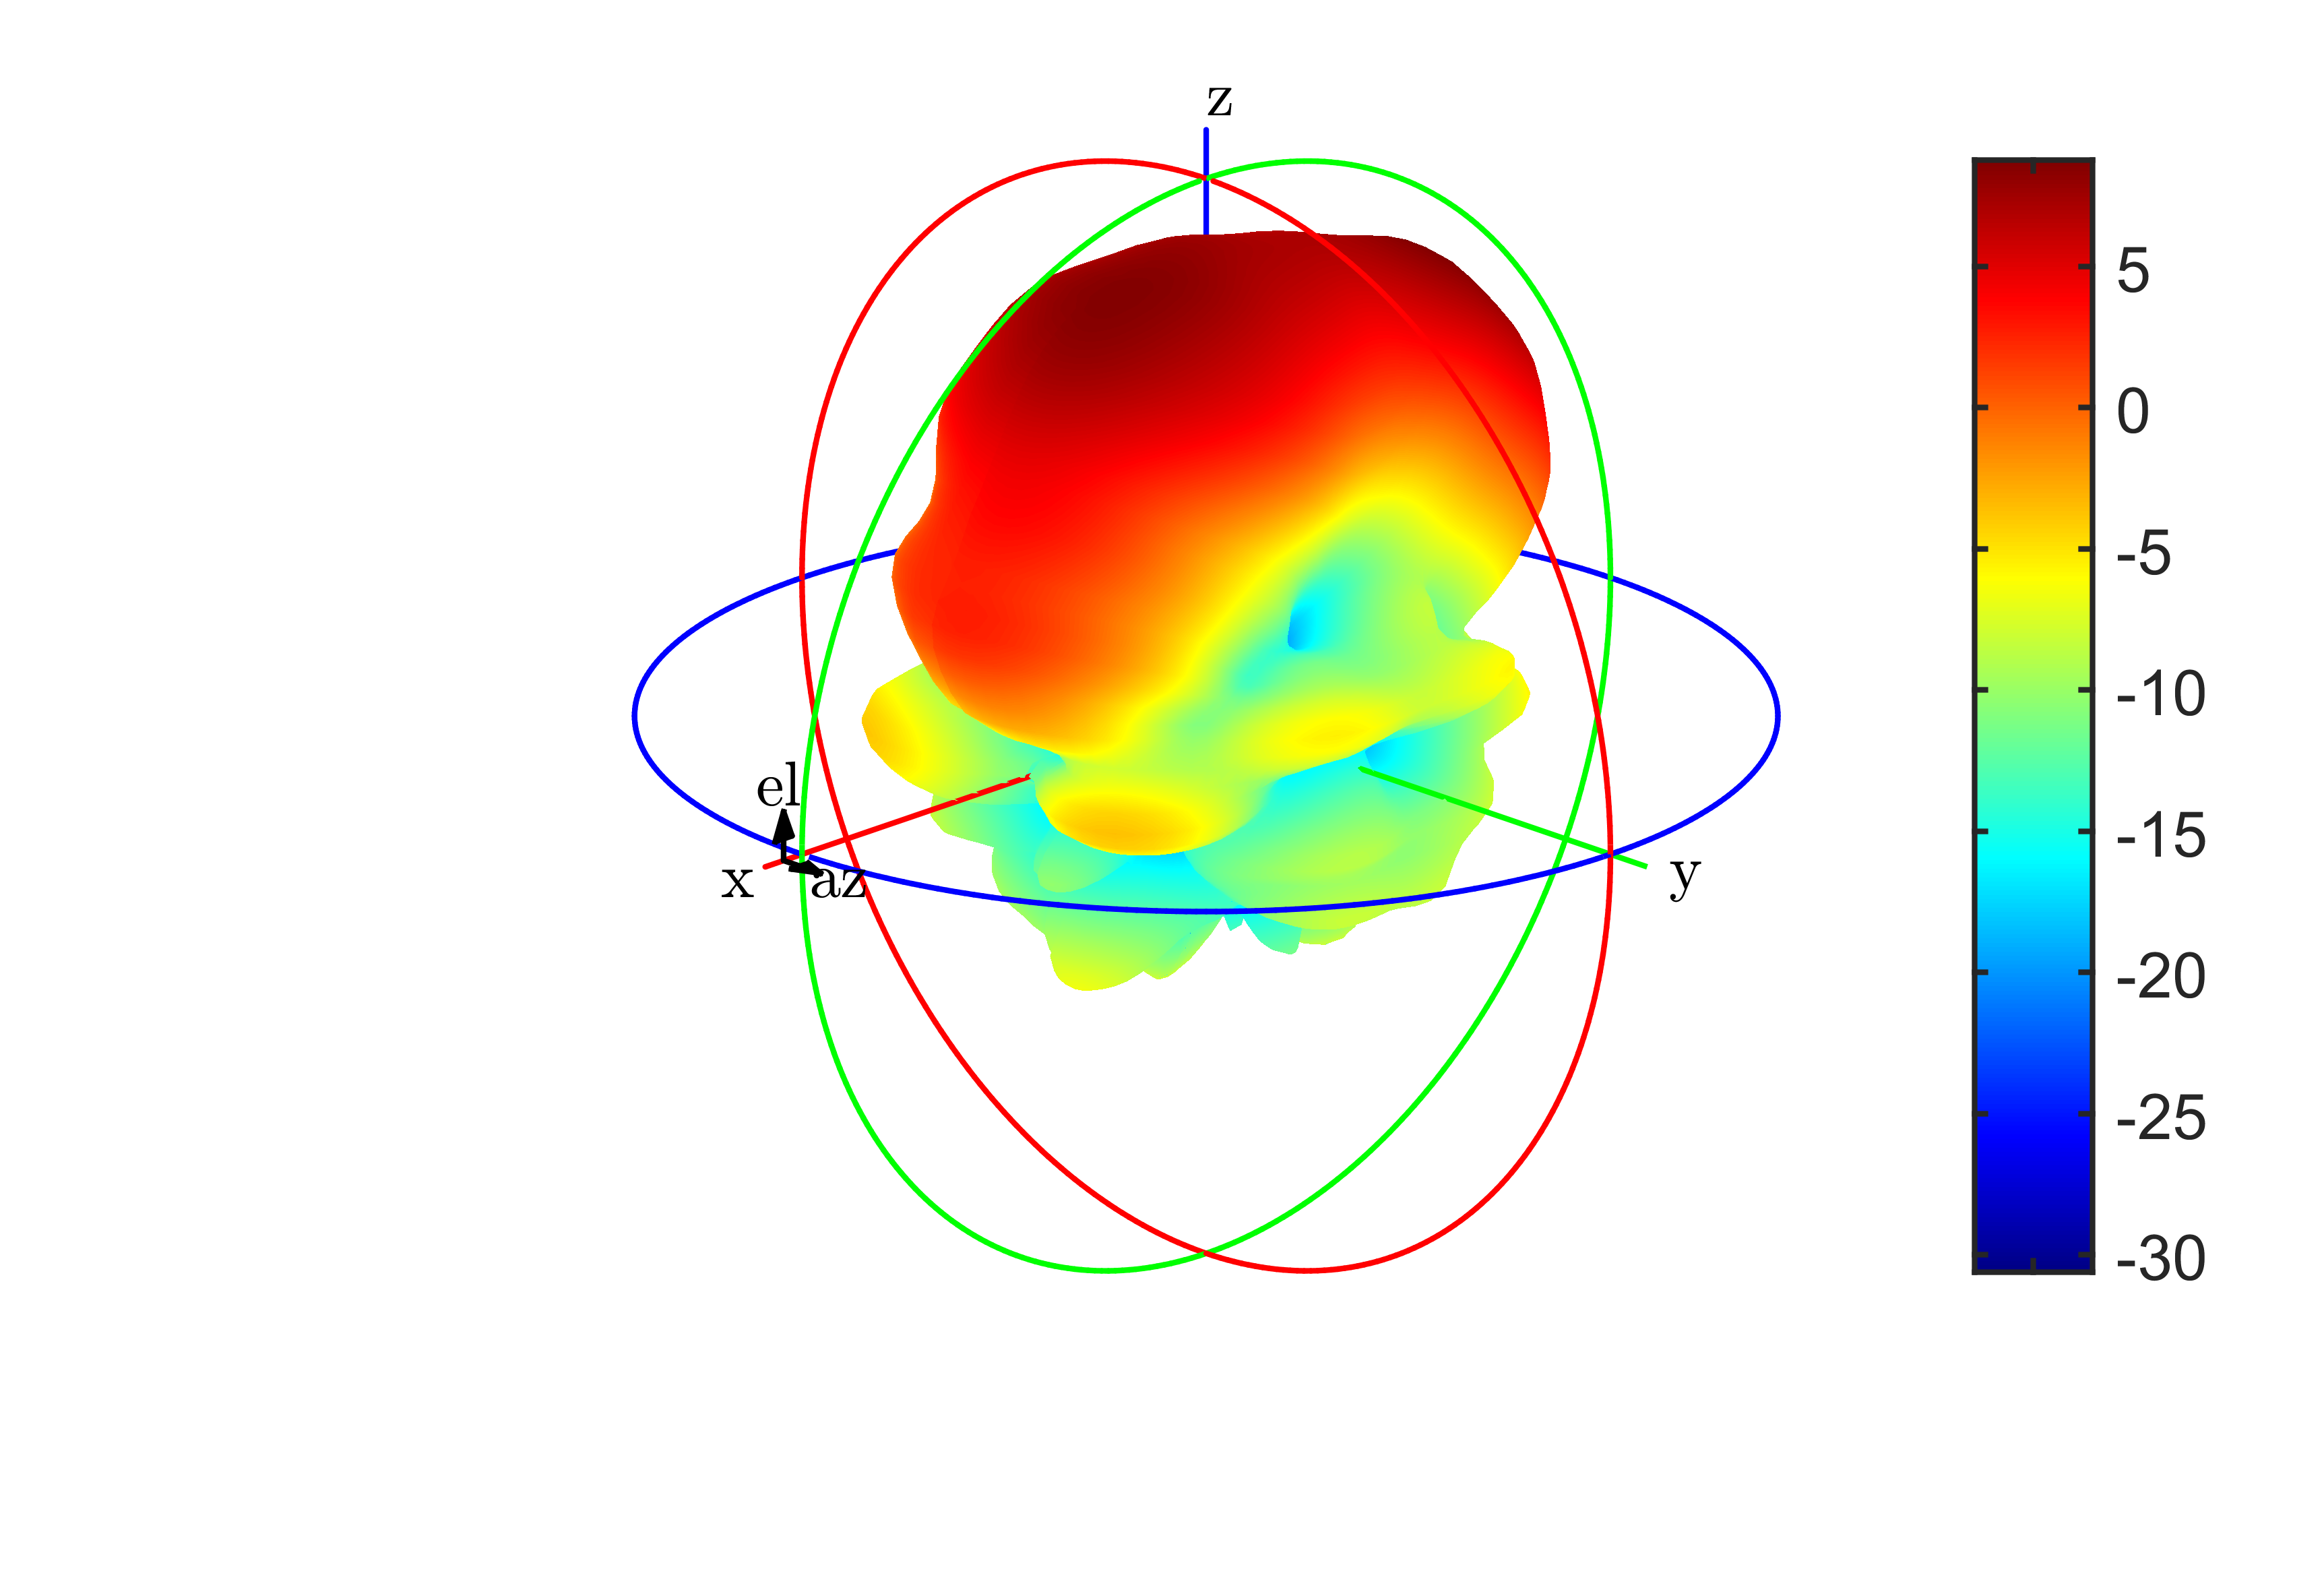
\includegraphics[scale = 0.5]{figures/measurement/antennas/3rd_element_4_array.png}
	\caption{Farfield third element in the four element array. Maximum gain is 8.8dB}
    \label{fig:chamber_four_ant_ff_3}
  \end{minipage}
  \hfill
  \begin{minipage}[b]{0.4\textwidth}
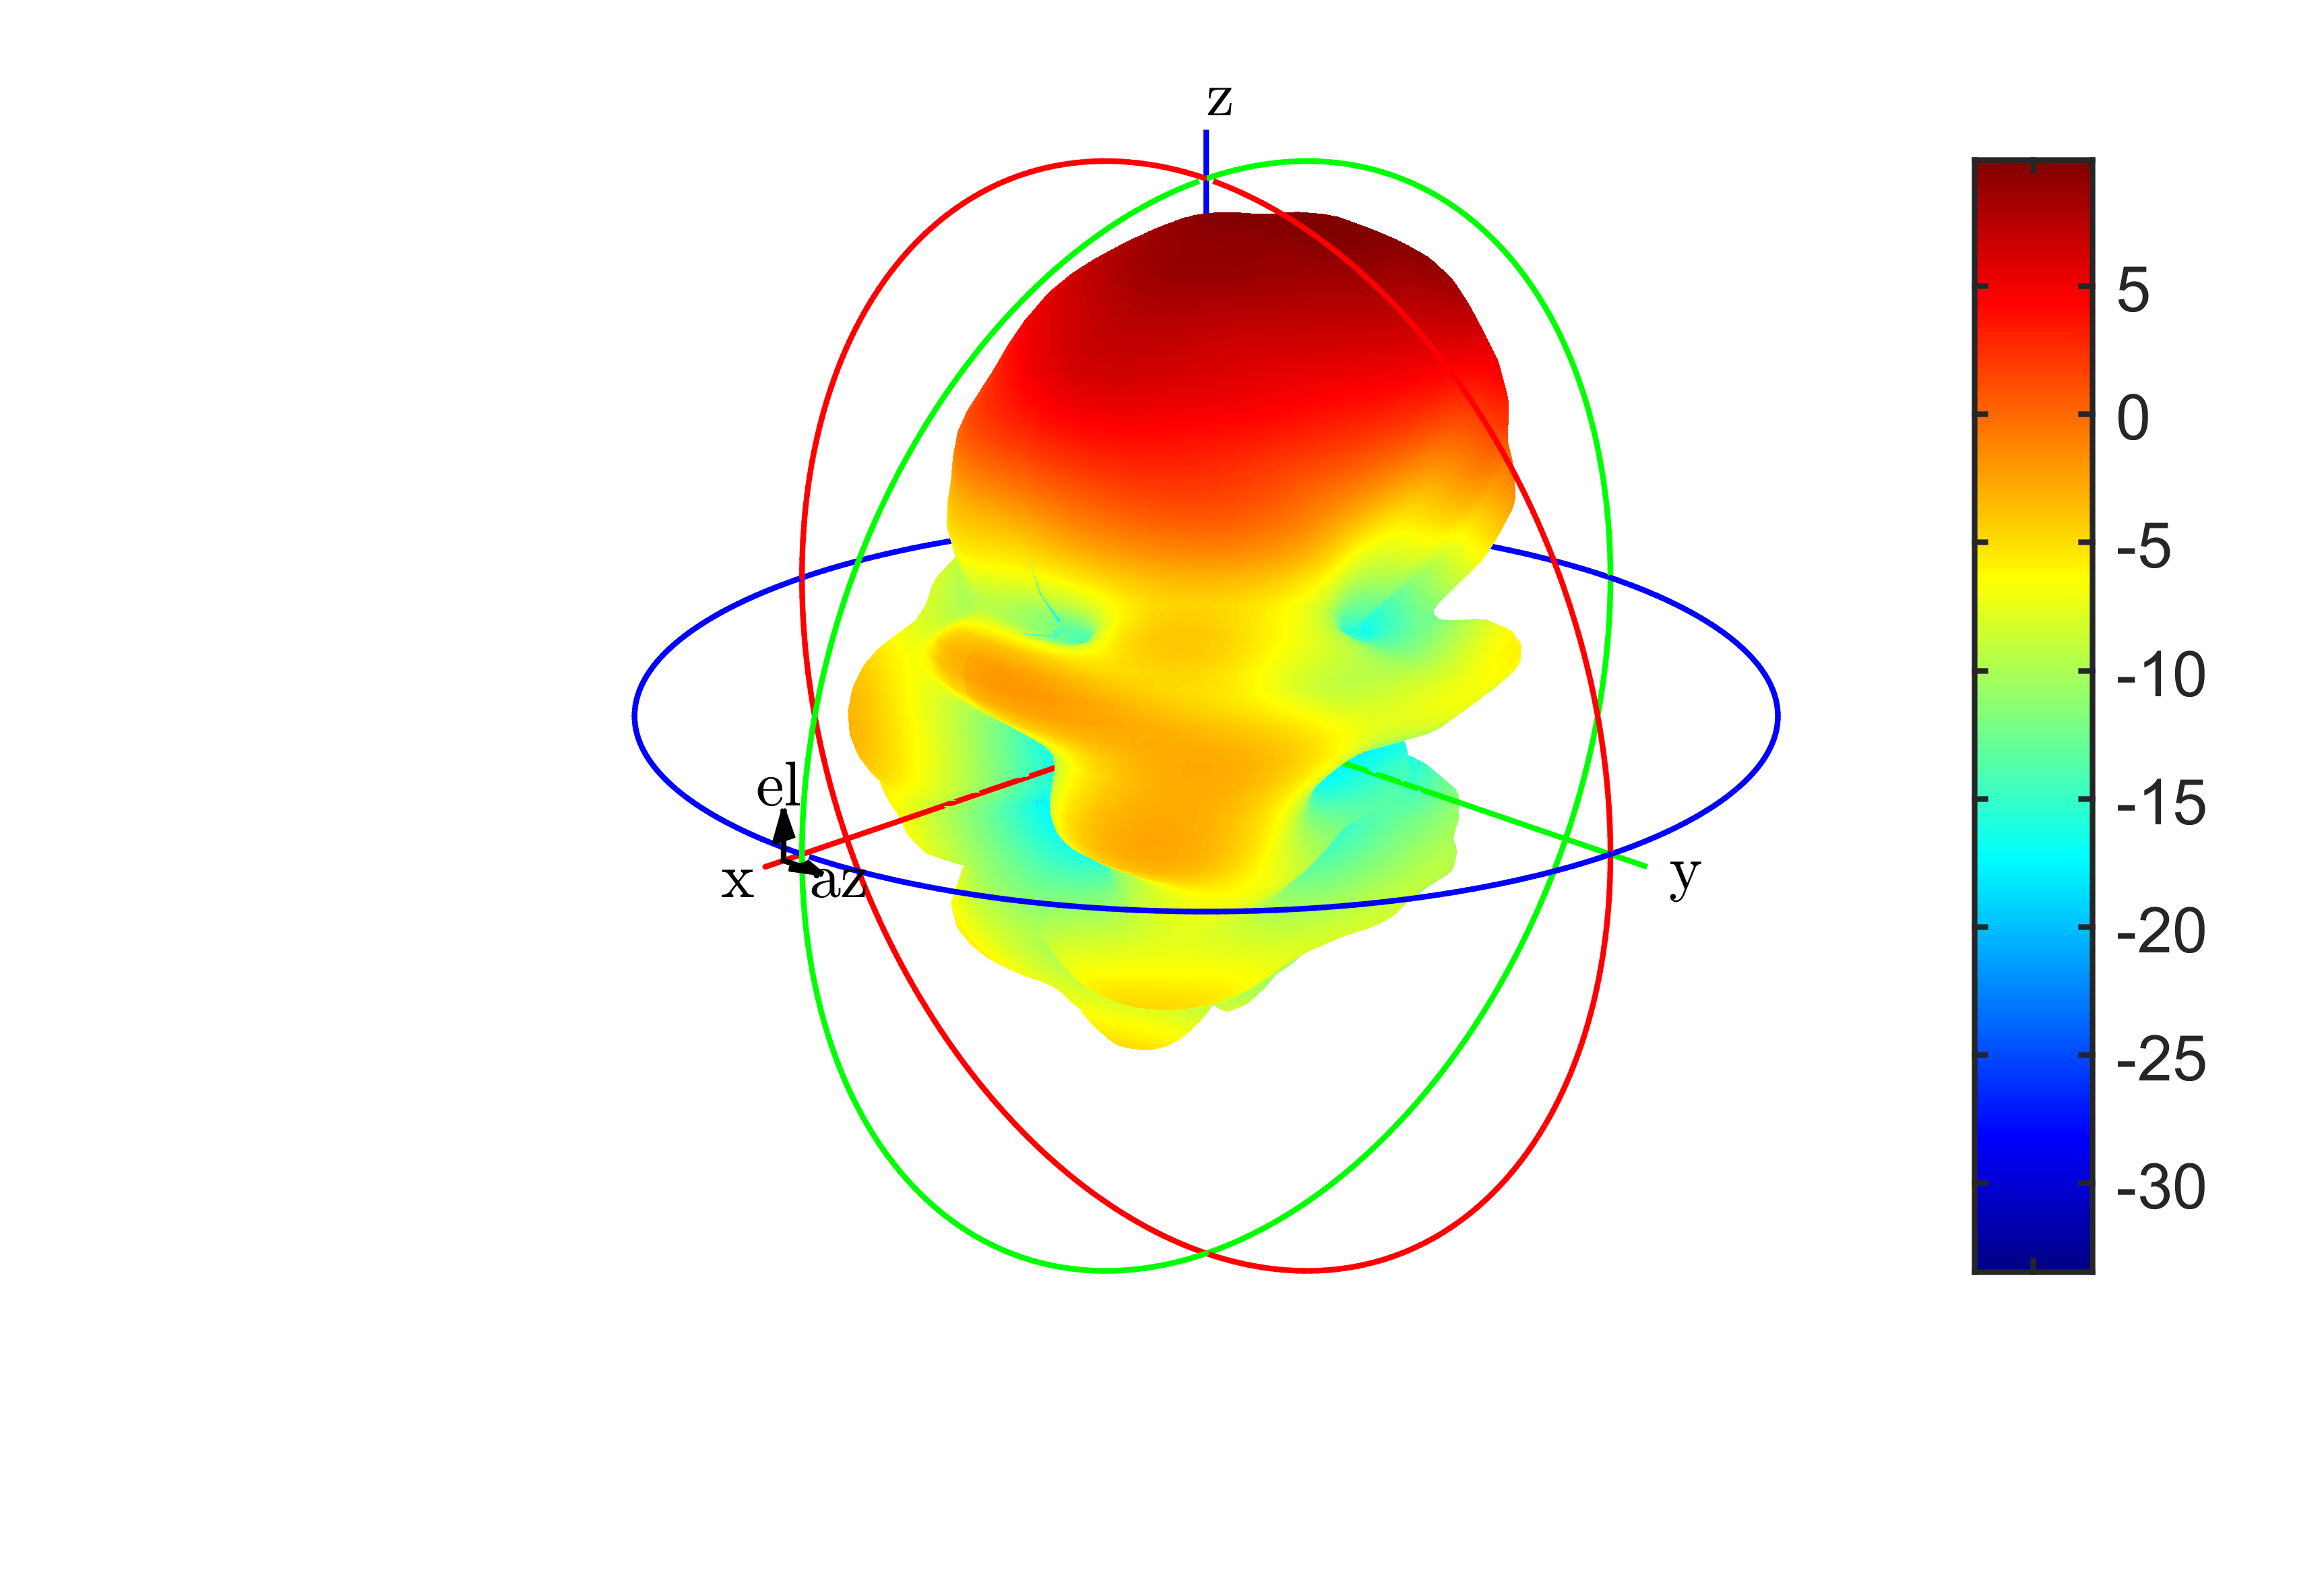
\includegraphics[scale = 0.5]{figures/measurement/antennas/4th_element_4_array.png}
\caption{Farfield fourth element in the four element array. Maximum gain is 9.9dB}
    \label{fig:chamber_four_ant_ff_4}
  \end{minipage}
\end{figure}










